
\newpage
\section{Numerical results}%
\label{sec:numerical_results}


To validate the proposed CutCIP method for the biharmonic problem will we investigate several numerical results both for the Laplace and Hessian formulation. From the theoretical optimal a priori estimates presented in presented in Theorem \ref{thm:apriori_result} will we provide examples where it holds. We also demonstrate the effect ghost penalty of stabilization by translating the domain to trigger badly cut cells. Finally, we provide numerical validation of the expected convergence for
the Cahn-Hilliard problem. We propose the following penalty parameters $\gamma = 20$ for the Hessian formulation \eqref{eq:hessian_prob} and the Laplace formulation \eqref{eq:laplace_prob}, and $\gamma _{1}, \gamma _{2} = 10, 0.5$ for the
corresponding ghost penalty \eqref{eq:ghost_penalty}.

Condition numbers are essential to solve linear systems because they help us assess the accuracy and stability of the system's solutions. A large condition number indicates that the system is ill-conditioned, meaning the solution can be highly
sensitive to small changes in the input data, potentially leading to inaccurate results. This underline the importance checking the conditional stability of cut cells, hence, motivating to do a so-called translation test with and without ghost
penalty.

\subsection{Convergence study for the cut finite element method method for the Biharmonic Problem  }%
\label{sub:numerical_results_for_cutcip_biharmonic_equation}
For the convergence study will we consider a square background domain $\widetilde{\Omega} $ with side lengths $L$ and a physical domain $\Omega \subset \widetilde{\Omega}$ on the form $\Omega  = \left\{ ( x,y)  \mid \phi ( x,y) \le 0    \right\} $,
where $\phi: \mathbb{R} ^2 \to \mathbb{R}  $ is a given level set function. We will consider two cases; a circular domain,
\begin{equation}
    \label{eq:circle}
\phi( x,y) = x^{ 2} + y^{2} -1
\end{equation}
and a flower shaped domain,
\begin{equation}
\label{eq:flower}
\phi ( x,y) =\sqrt{x^{2} + y^{2}} - r_{0} - r_{1}\cos(\atantwo(y,x)) \text{ where }  r_{0} = 0.3L  \text{ and } \ r_{1} = 0.1L .
\end{equation}
For an illustration of the flower domain, see Figure \ref{fig:flower}.

\begin{figure}[h!]
    \centering
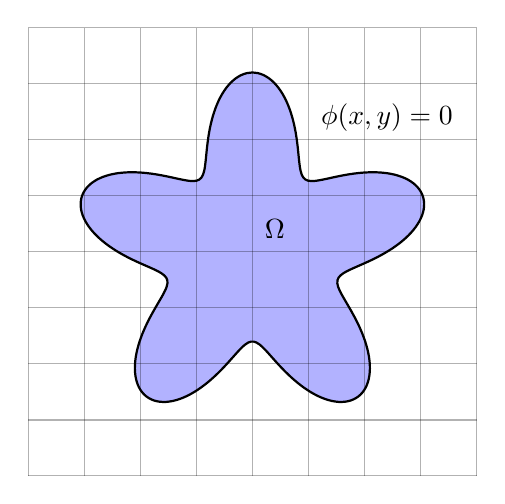
\begin{tikzpicture}
  \def\rZero{0.6} % Define r_0
  \def\rOne{0.2} % Define r_1
  \begin{axis}[
    xmin=-1, xmax=1,
    ymin=-1, ymax=1,
    axis lines=center,
    axis equal,
    hide axis,  % This will hide the axis
    % xlabel={$x$},
    % ylabel={$y$},
    % grid=both,
    % minor tick num=1,
    domain=0:2*pi,
    samples=200
  ]

  \addplot[thick, parametric, smooth, fill=blue!30] ({(\rZero + \rOne*cos(5*deg(x)))*sin(deg(x))} , {(\rZero + \rOne*cos(5*deg(x)))*cos(deg(x))});
  \node at (0.1, 0.1) {$\Omega$};
  \node at (0.6, 0.6) {$\phi( x,y ) = 0 $};

  % Background mesh
  \foreach \i in {-1, -0.75, ..., 1} {
      \addplot[ thin, opacity=0.3, forget plot] coordinates {(\i,-1) (\i,1)};
      \addplot[ thin, opacity=0.3, forget plot] coordinates {(-1,\i) (1,\i)};
  }

  \end{axis}
\end{tikzpicture}
\caption{Illustration of the flower domain associated with the level set function \eqref{eq:flower}.}
    \label{fig:flower}
\end{figure}


We want to test spatial convergence for the method by doing a numerous of mesh refinements. Let $ \widetilde{\mathcal{T}}_{h}^{k} $ be the associated regular square mesh of the background domain $\widetilde{\Omega }$ with the mesh size  $h^{k} = L/2^{3+k} $
for the side length $L=2.7$ and refinements
$k=0, \ldots, 6$. For the circular domain is this illustrated in the Figure \ref{fig:refinement}.

\begin{figure}[hpbt!]
    \centering
\subfloat[]{\label{sub:fig:refine_a}
        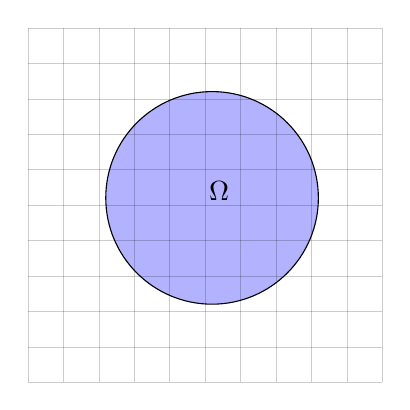
\begin{tikzpicture}[scale=0.9]

            % Domain is blue
            \fill[blue!30] (0.1, 0.1) circle (1.5cm);
            \draw[black] (0.1, 0.1) circle (1.5cm);
            \node at (0.2, 0.2) {$\Omega$};

            % Background mesh
            \foreach \i in {-2.5, -2, ..., 2.5} {
                \draw[line width=0.1pt, shift={(-2.5,\i)}, opacity=0.2] (0,0) -- (5,0);
                \draw[line width=0.1pt, shift={(\i,-2.5)},opacity=0.2] (0,0) -- (0,5);
            }

        \end{tikzpicture}

}\hfill
\subfloat[]{\label{sub:fig:refine_b}
        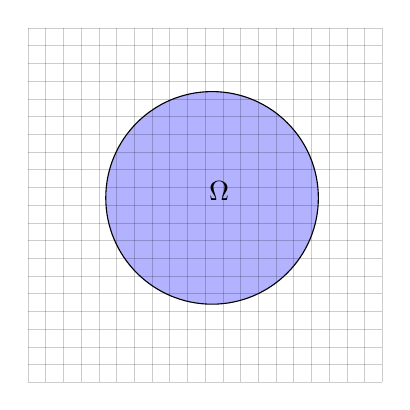
\begin{tikzpicture}[scale=0.9]

            % Domain is blue
            \fill[blue!30] (0.1, 0.1) circle (1.5cm);
            \draw[black] (0.1, 0.1) circle (1.5cm);
            \node at (0.2, 0.2) {$\Omega$};

            % Background mesh
            \foreach \i in {-2.5, -2.25, ..., 2.5} {
                \draw[line width=0.1pt, shift={(-2.5,\i)}, opacity=0.2] (0,0) -- (5,0);
                \draw[line width=0.1pt, shift={(\i,-2.5)},opacity=0.2] (0,0) -- (0,5);
            }

        \end{tikzpicture}


}
\hfill
\subfloat[]{\label{sub:fig:refine_c}
        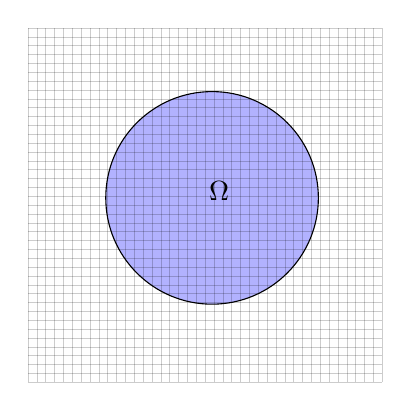
\begin{tikzpicture}[scale=0.9]

            % Domain is blue
            \fill[blue!30] (0.1, 0.1) circle (1.5cm);
            \draw[black] (0.1, 0.1) circle (1.5cm);
            \node at (0.2, 0.2) {$\Omega$};

            % Background mesh
            \foreach \i in {-2.5, -2.375, ..., 2.5} {
                \draw[line width=0.1pt, shift={(-2.5,\i)}, opacity=0.2] (0,0) -- (5,0);
                \draw[line width=0.1pt, shift={(\i,-2.5)},opacity=0.2] (0,0) -- (0,5);
            }

        \end{tikzpicture}
}
    \caption{Illustration of the domain $\Omega $ defined as a circle with radius $R$. The regular square background mesh $ \widetilde{\mathcal{T}}_{h}^{k} $ with side lengths $L$ with three refinements of the mesh size $h^{k}$.}
    \label{fig:refinement}
\end{figure}

On each mesh $\widetilde{\mathcal{T}}^{k}_{h}  $ we compute a numerical solution $u_{h}^{k}$, hence, motivating us to define the convergence rate. Let $u $ be the exact solution, then do we define the so-called Experimental Order of Convergence (EOC) as \[
EOC( k) =  \frac{\log \left(  \frac{e^{k-1}}{e^{k}} \right)}{\log \left(  \frac{h^{k-1}}{h^{k}} \right)}, \quad    k>0
\]
Here we define the error $e^{k} = \| u - u_{h}^{k} \|_{  }^{  } $, where we choose to measure in the norms $ \|\cdot   \|_{L^2( \Omega )   }^{  },   \|\cdot   \|_{H^1( \Omega )   }^{  } $ and $ \|\cdot   \|_{ a_{h},* }^{  }$.

\subsection{Note on the condition number}%
\label{sub:note_on_condition_number}


Recall that $V_{h} $ is spanned by the polynomial basis $\left\{ \phi _{1}, \ldots, \phi _{N}  \right\} $ such that $dim(V_{h}) = N$, where $N$ is the so-called number of degrees of freedom (ndofs). From basic theory
do we know that we can span the discrete solution s.t.
$u_{h} = \sum_{i=1}^{N}  U_{i} \phi_{i} $ with coefficients $\left\{
U_{i}\right\} _{i=1}^{N}$ and the stiffness matrix $\left[ A  \right] _{ji} = a_{h}( \phi _{i}, \phi _{j}) $ and vector $\left[ F \right] _{j} = l_{h}( \phi_{j} ) $. Thus, we have the following equivalent linear system of the problem finding a $u_{h} \in  V_{h}$ s.t.
$a_{h}( u_{h},v_{h})  = l_{h}( v_{h}) \forall v_{h} \in V_{h}$, that is, to find a $U \in \mathbb{R} ^{N}$ s.t. $AU =F$. We may recall the discrete $l^{p}$ norm, i.e.,\(
    \| U  \|_{ p }^{  } = \sum_{i=1}^{N}  \abs{ U_{i}  } \text{ for } U \in \mathbb{R} ^{N}
\)
where $1\le p < \infty$ and $\| U \|_{ \infty }^{  }  = \max_{i}  \abs{ U_i } $.
Remark that this notation is not to be confused with Sobolev norms.
Also recall the definition of the matrix norm, \[
\| A  \|_{p  }^{  }  = \max_{U \in \mathbb{R} ^{N} \setminus 0} \frac{\| AU \|_{ p }^{  } }{\| U \|_{p}^{  } } \text{ for } A \in \mathbb{R} ^{N\times N}.
\]
Assume that $A $ is invertible, then we define the condition number for a matrix in $l^{p}  $ norm defined s.t. \[
\kappa_{p} ( A) = \| A  \|_{ p }^{  } \| A ^{-1} \|_{ p }  .
\]
Because of the connection of $l^{2}$ norms of a matrix and its eigenvalues is $k_{2}( A) $ preferred in most cases numerical analysis. However, from linear algebra is a well known result that $ \frac{1}{\sqrt{N} }  \| A \|_{ \infty }^{  }  \le \| A \|_{2  }^{  } \le
\sqrt{N}  \| A \|_{\infty  }^{  }  $ for any matrix $A \in R^{N\times N}$  \footnote{
    The identity naturally appears from the standard inequality $\| v \|_{ \infty }^{  } \le  \| v \|_{2  }^{  } \le \sqrt{N}  \| v \|_{ \infty }^{  }   $ for $v \in R^{N}$, which simply comes from the fact that  $ \| v \|_{\infty  }^{ 2 } = \max_{i} \abs{ v_{i} }^{2} \le \sum_{i}^{n}   \abs{ v_{i} }^{2} = \| v \|_{ 2 }^{2  } \le N      \max_{i} \abs{ v_{i} }^{2} = N \| v \|_{
    \infty}^{ 2 }$. Now let $A\in \mathbb{R} ^{N \times N}$ be any matrix. We can then deduce that $ \| A \|_{ 2 }^{  } = \max_{v \in \mathbb{R} ^{N}} \frac{\| Av \|_{2  }^{  }}{\| v \|_{ 2 }^{  } } \ge \max_{v \in \mathbb{R} ^{N}}
    \frac{\| Av \|_{ \infty  }^{  }}{ \sqrt{N} \| v \|_{ \infty}^{  } } = \frac{1}{ \sqrt{N} } \| A \|_{ \infty }^{  }    $ and $ \| A \|_{ 2 }^{  } = \max_{v \in \mathbb{R} ^{N}} \frac{\| Av \|_{2  }^{  }}{\| v \|_{ 2 }^{  } } \le  \max_{v \in \mathbb{R} ^{N}}
    \frac{\sqrt{N} \| Av \|_{ \infty  }^{  }}{  \| v \|_{ \infty}^{  } } =  \sqrt{N} \| A \|_{ \infty }^{  }    $. Hence, the identity $\frac{1}{\sqrt{N} } \| A \|_{\infty  }^{  } \le \| A \|_{ 2 }^{  }\le \sqrt{N} \| A \|_{ \infty  }^{  }   $  is proven.

}. Using this fact, do we have a upper and lower limit of the condition number ,
\[
\frac{1}{N} \kappa_{\infty} ( A) \le  \kappa_{2} ( A) \le N \kappa _{\infty}(A)    .
\]
Thus, since these norms are equivalent will we in this report focus on $ \kappa_{\infty}( A)  $.
\begin{remark}
 The $l^{\infty}$ is computed as the maximum absolute row sum of the matrix. For a sparse matrix, you only need to calculate the sum for the non-zero elements in each row, so computing the infinity norm can be very efficient for a sparse matrix. The
 $l^{2}$ norm, on the other hand, is not so straightforward to calculate. For a matrix A, is the $l^{2}$ -norm is the square root of the maximum eigenvalue of $A^T  A$. Computing this generally involves performing Singular Value Decomposition (SVD)
 or power iteration, which can be quite expensive operations, particularly for large matrices.
\end{remark}

\subsection{Validation of the a priori estimates }%
\label{ssub:numerical_results}

Our goal it validate the Theorem \ref{thm:apriori_result} for $k= 2$ for the Hessian formulation and show that the Laplace formulation has the same properties.
The big-oh $O( h^{r})$ is defined to be to be a upper bound such that it exists an $C>0$ such that $\| e \|_{  }^{  } \le C h^{r} \text{ for all } h$, where $r$ is the order of convergence. Since we only will implement $k=2$, we validate that it exists an upper bound $ O( h)  $ for  $\| e \|_{L^{2}( \Omega )   }^{  }$  and $O( h^2)  $ for $\| e \|_{ a_{h},* }^{  } $.
It has also been shown that for condition number $\kappa_{\infty} ( A) $  increases with the order of $O( h^{-4}) $\cite{li07}, hence, we expect this to hold for both methods as well.
We did the following convergence tests.
\begin{itemize}
    \item \textbf{Convergence on circle domain}
        First we consider the manufactured solution s.t.
        \begin{equation}
        \label{eq:man_sol_1}
            u(x,y) = (x^2+ y^2 -1) \sin\left(2 \pi x \right)\cos\left(2\pi y\right)
        \end{equation}
        The result can be shown on the in Figure \ref{fig:conv_hes_lap} and Table \ref{tab:conv_hes_lap}. Here we observe that for we clearly get optimal convergence, that is, we get a consistent EOC 1 and 2 for the respective norms $\| e  \|_{a_{h},*  }^{  } $
        and $\| e  \|_{L^2( \Omega )   }^{  } $.  We also get a consistent EOC of 2 for $\| e \|_{ H^{1}(\Omega  )  }^{  } $, even though we do not have theoretical a priori estimates of this norm.
        We also see that the condition number $\kappa _{\infty}( A)  $ has a expected
        convergence of $-4$ and, thus, for small $h\le \frac{1}{512}$ we see a drop in convergence rate.
    \item \textbf{Convergence on flower domain}
        We consider the manufactured solution such that
        \begin{equation}
        \label{eq:man_sol_2}
            u(x,y) =  \sin\left( 2\pi x \right)\cos\left(2\pi y\right)
        \end{equation}
        In this case must we assume non homogeneous Neumann conditions, and thus we only test the numerical results for the Laplace formulation. The result can be shown on the in Figure \ref{fig:conv_flower_lap} and Table \ref{tab:conv_flower_lap}. Here we
        observe that for we get optimal convergence, that is EOC of order 1 and 2 for $\| e  \|_{a_{h},*  }^{  } $ and  $ \| e  \|_{L^{2}( \Omega )   }^{  } $ norm. Again, we see that the condition number $\kappa _{\infty}( A)  $ has a EOC of order
        $-4$ and, thus, for small $h\le \frac{1}{512}$ we see a drop in convergence rate for the $\| e_{h} \|_{ L^{2} }^{  } $ norm.
\end{itemize}

\begin{figure}[h!]
\centering
\subfloat[Hessian]{% Recommended preamble:
% \usetikzlibrary{arrows.meta}
% \usetikzlibrary{backgrounds}
% \usepgfplotslibrary{patchplots}
% \usepgfplotslibrary{fillbetween}
% \pgfplotsset{%
%     layers/standard/.define layer set={%
%         background,axis background,axis grid,axis ticks,axis lines,axis tick labels,pre main,main,axis descriptions,axis foreground%
%     }{
%         grid style={/pgfplots/on layer=axis grid},%
%         tick style={/pgfplots/on layer=axis ticks},%
%         axis line style={/pgfplots/on layer=axis lines},%
%         label style={/pgfplots/on layer=axis descriptions},%
%         legend style={/pgfplots/on layer=axis descriptions},%
%         title style={/pgfplots/on layer=axis descriptions},%
%         colorbar style={/pgfplots/on layer=axis descriptions},%
%         ticklabel style={/pgfplots/on layer=axis tick labels},%
%         axis background@ style={/pgfplots/on layer=axis background},%
%         3d box foreground style={/pgfplots/on layer=axis foreground},%
%     },
% }

\begin{tikzpicture}[/tikz/background rectangle/.style={fill={rgb,1:red,1.0;green,1.0;blue,1.0}, fill opacity={1.0}, draw opacity={1.0}}, show background rectangle]
\begin{axis}[point meta max={nan}, point meta min={nan}, legend cell align={left}, legend columns={1}, title={}, title style={at={{(0.5,1)}}, anchor={south}, font={{\fontsize{14 pt}{18.2 pt}\selectfont}}, color={rgb,1:red,0.0;green,0.0;blue,0.0}, draw opacity={1.0}, rotate={0.0}, align={center}}, legend style={color={rgb,1:red,0.0;green,0.0;blue,0.0}, draw opacity={1.0}, line width={1}, solid, fill={rgb,1:red,1.0;green,1.0;blue,1.0}, fill opacity={1.0}, text opacity={1.0}, font={{\fontsize{12 pt}{15.600000000000001 pt}\selectfont}}, text={rgb,1:red,0.0;green,0.0;blue,0.0}, cells={anchor={center}}, at={(1.02, 1)}, anchor={north west}}, axis background/.style={fill={rgb,1:red,1.0;green,1.0;blue,1.0}, opacity={1.0}}, anchor={north west}, xshift={1.0mm}, yshift={-1.0mm}, width={145.4mm}, height={61.5mm}, scaled x ticks={false}, xlabel={h}, x tick style={color={rgb,1:red,0.0;green,0.0;blue,0.0}, opacity={1.0}}, x tick label style={color={rgb,1:red,0.0;green,0.0;blue,0.0}, opacity={1.0}, rotate={0}}, xlabel style={at={(ticklabel cs:0.5)}, anchor=near ticklabel, at={{(ticklabel cs:0.5)}}, anchor={near ticklabel}, font={{\fontsize{11 pt}{14.3 pt}\selectfont}}, color={rgb,1:red,0.0;green,0.0;blue,0.0}, draw opacity={1.0}, rotate={0.0}}, xmode={log}, log basis x={2}, xmajorgrids={true}, xmin={0.0034480585792603714}, xmax={0.2832209713239497}, xticklabels={{$2^{-6}$,$2^{-3}$}}, xtick={{0.015625,0.125}}, xtick align={inside}, xticklabel style={font={{\fontsize{8 pt}{10.4 pt}\selectfont}}, color={rgb,1:red,0.0;green,0.0;blue,0.0}, draw opacity={1.0}, rotate={0.0}}, x grid style={color={rgb,1:red,0.0;green,0.0;blue,0.0}, draw opacity={0.1}, line width={0.5}, solid}, axis x line*={left}, x axis line style={color={rgb,1:red,0.0;green,0.0;blue,0.0}, draw opacity={1.0}, line width={1}, solid}, scaled y ticks={false}, ylabel={}, y tick style={color={rgb,1:red,0.0;green,0.0;blue,0.0}, opacity={1.0}}, y tick label style={color={rgb,1:red,0.0;green,0.0;blue,0.0}, opacity={1.0}, rotate={0}}, ylabel style={at={(ticklabel cs:0.5)}, anchor=near ticklabel, at={{(ticklabel cs:0.5)}}, anchor={near ticklabel}, font={{\fontsize{11 pt}{14.3 pt}\selectfont}}, color={rgb,1:red,0.0;green,0.0;blue,0.0}, draw opacity={1.0}, rotate={0.0}}, ymode={log}, log basis y={2}, ymajorgrids={true}, ymin={2.134188856671611e-5}, ymax={39.36726929884525}, yticklabels={{$2^{-8}$,$2^{0}$}}, ytick={{0.00390625,1.0}}, ytick align={inside}, yticklabel style={font={{\fontsize{8 pt}{10.4 pt}\selectfont}}, color={rgb,1:red,0.0;green,0.0;blue,0.0}, draw opacity={1.0}, rotate={0.0}}, y grid style={color={rgb,1:red,0.0;green,0.0;blue,0.0}, draw opacity={0.1}, line width={0.5}, solid}, axis y line*={left}, y axis line style={color={rgb,1:red,0.0;green,0.0;blue,0.0}, draw opacity={1.0}, line width={1}, solid}, colorbar={false}]
    \addplot[color={rgb,1:red,0.0;green,0.6056;blue,0.9787}, name path={ec49766f-1a90-48e0-b04d-b95058e7ee06}, draw opacity={1.0}, line width={1}, solid]
        table[row sep={\\}]
        {
            \\
            0.25  0.1786123712821028  \\
            0.125  0.038644947655226136  \\
            0.0625  0.009127774348082682  \\
            0.03125  0.002185541896939916  \\
            0.015625  0.0005265553342003825  \\
            0.0078125  0.0001293181160260665  \\
            0.00390625  3.210478083835641e-5  \\
        }
        ;
    \addlegendentry {$\Vert e \Vert_{L^2}$}
    \addplot[color={rgb,1:red,0.0;green,0.6056;blue,0.9787}, name path={f910c76a-f2ed-4fd3-bc50-cf717f11e66e}, only marks, draw opacity={1.0}, line width={0}, solid, mark={*}, mark size={3.0 pt}, mark repeat={1}, mark options={color={rgb,1:red,0.0;green,0.0;blue,0.0}, draw opacity={1.0}, fill={rgb,1:red,0.0;green,0.6056;blue,0.9787}, fill opacity={1.0}, line width={0.75}, rotate={0}, solid}, forget plot]
        table[row sep={\\}]
        {
            \\
            0.25  0.1786123712821028  \\
            0.125  0.038644947655226136  \\
            0.0625  0.009127774348082682  \\
            0.03125  0.002185541896939916  \\
            0.015625  0.0005265553342003825  \\
            0.0078125  0.0001293181160260665  \\
            0.00390625  3.210478083835641e-5  \\
        }
        ;
    \addplot[color={rgb,1:red,0.8889;green,0.4356;blue,0.2781}, name path={bd5609d7-3aec-41b7-ac39-f3440829a058}, draw opacity={1.0}, line width={1}, solid]
        table[row sep={\\}]
        {
            \\
            0.25  1.875795347934765  \\
            0.125  0.475856282170078  \\
            0.0625  0.11696924139879772  \\
            0.03125  0.028655306235220564  \\
            0.015625  0.0068702390988027206  \\
            0.0078125  0.001683286234451497  \\
            0.00390625  0.00041457632061992655  \\
        }
        ;
    \addlegendentry {$\Vert e \Vert_{H^1}$}
    \addplot[color={rgb,1:red,0.8889;green,0.4356;blue,0.2781}, name path={96c807d6-fc37-482a-a851-53a600592b73}, only marks, draw opacity={1.0}, line width={0}, solid, mark={*}, mark size={3.0 pt}, mark repeat={1}, mark options={color={rgb,1:red,0.0;green,0.0;blue,0.0}, draw opacity={1.0}, fill={rgb,1:red,0.8889;green,0.4356;blue,0.2781}, fill opacity={1.0}, line width={0.75}, rotate={0}, solid}, forget plot]
        table[row sep={\\}]
        {
            \\
            0.25  1.875795347934765  \\
            0.125  0.475856282170078  \\
            0.0625  0.11696924139879772  \\
            0.03125  0.028655306235220564  \\
            0.015625  0.0068702390988027206  \\
            0.0078125  0.001683286234451497  \\
            0.00390625  0.00041457632061992655  \\
        }
        ;
    \addplot[color={rgb,1:red,0.2422;green,0.6433;blue,0.3044}, name path={90fe245b-d754-479d-b19e-aea2bc912a7b}, draw opacity={1.0}, line width={1}, solid]
        table[row sep={\\}]
        {
            \\
            0.25  26.16968104476466  \\
            0.125  11.928804161283171  \\
            0.0625  5.710074204166452  \\
            0.03125  2.8067545242047762  \\
            0.015625  1.3910287705325208  \\
            0.0078125  0.6930329020125815  \\
            0.00390625  0.34579918853976266  \\
        }
        ;
    \addlegendentry {$\Vert e \Vert_{a_{h,*}}$}
    \addplot[color={rgb,1:red,0.2422;green,0.6433;blue,0.3044}, name path={c5895967-c532-4b2f-aaac-a96a37d1fffe}, only marks, draw opacity={1.0}, line width={0}, solid, mark={*}, mark size={3.0 pt}, mark repeat={1}, mark options={color={rgb,1:red,0.0;green,0.0;blue,0.0}, draw opacity={1.0}, fill={rgb,1:red,0.2422;green,0.6433;blue,0.3044}, fill opacity={1.0}, line width={0.75}, rotate={0}, solid}, forget plot]
        table[row sep={\\}]
        {
            \\
            0.25  26.16968104476466  \\
            0.125  11.928804161283171  \\
            0.0625  5.710074204166452  \\
            0.03125  2.8067545242047762  \\
            0.015625  1.3910287705325208  \\
            0.0078125  0.6930329020125815  \\
            0.00390625  0.34579918853976266  \\
        }
        ;
\end{axis}
\end{tikzpicture}
}
% \hfill
\subfloat[Laplace]{% Recommended preamble:
% \usetikzlibrary{arrows.meta}
% \usetikzlibrary{backgrounds}
% \usepgfplotslibrary{patchplots}
% \usepgfplotslibrary{fillbetween}
% \pgfplotsset{%
%     layers/standard/.define layer set={%
%         background,axis background,axis grid,axis ticks,axis lines,axis tick labels,pre main,main,axis descriptions,axis foreground%
%     }{
%         grid style={/pgfplots/on layer=axis grid},%
%         tick style={/pgfplots/on layer=axis ticks},%
%         axis line style={/pgfplots/on layer=axis lines},%
%         label style={/pgfplots/on layer=axis descriptions},%
%         legend style={/pgfplots/on layer=axis descriptions},%
%         title style={/pgfplots/on layer=axis descriptions},%
%         colorbar style={/pgfplots/on layer=axis descriptions},%
%         ticklabel style={/pgfplots/on layer=axis tick labels},%
%         axis background@ style={/pgfplots/on layer=axis background},%
%         3d box foreground style={/pgfplots/on layer=axis foreground},%
%     },
% }

\begin{tikzpicture}[/tikz/background rectangle/.style={fill={rgb,1:red,1.0;green,1.0;blue,1.0}, fill opacity={1.0}, draw opacity={1.0}}, show background rectangle]
\begin{axis}[point meta max={nan}, point meta min={nan}, legend cell align={left}, legend columns={1}, title={}, title style={at={{(0.5,1)}}, anchor={south}, font={{\fontsize{14 pt}{18.2 pt}\selectfont}}, color={rgb,1:red,0.0;green,0.0;blue,0.0}, draw opacity={1.0}, rotate={0.0}, align={center}}, legend style={color={rgb,1:red,0.0;green,0.0;blue,0.0}, draw opacity={1.0}, line width={1}, solid, fill={rgb,1:red,1.0;green,1.0;blue,1.0}, fill opacity={1.0}, text opacity={1.0}, font={{\fontsize{12 pt}{15.600000000000001 pt}\selectfont}}, text={rgb,1:red,0.0;green,0.0;blue,0.0}, cells={anchor={center}}, at={(1.02, 1)}, anchor={north west}}, axis background/.style={fill={rgb,1:red,1.0;green,1.0;blue,1.0}, opacity={1.0}}, anchor={north west}, xshift={1.0mm}, yshift={-1.0mm}, width={145.4mm}, height={61.5mm}, scaled x ticks={false}, xlabel={h}, x tick style={color={rgb,1:red,0.0;green,0.0;blue,0.0}, opacity={1.0}}, x tick label style={color={rgb,1:red,0.0;green,0.0;blue,0.0}, opacity={1.0}, rotate={0}}, xlabel style={at={(ticklabel cs:0.5)}, anchor=near ticklabel, at={{(ticklabel cs:0.5)}}, anchor={near ticklabel}, font={{\fontsize{11 pt}{14.3 pt}\selectfont}}, color={rgb,1:red,0.0;green,0.0;blue,0.0}, draw opacity={1.0}, rotate={0.0}}, xmode={log}, log basis x={2}, xmajorgrids={true}, xmin={0.0034480585792603714}, xmax={0.2832209713239497}, xticklabels={{$2^{-6}$,$2^{-3}$}}, xtick={{0.015625,0.125}}, xtick align={inside}, xticklabel style={font={{\fontsize{8 pt}{10.4 pt}\selectfont}}, color={rgb,1:red,0.0;green,0.0;blue,0.0}, draw opacity={1.0}, rotate={0.0}}, x grid style={color={rgb,1:red,0.0;green,0.0;blue,0.0}, draw opacity={0.1}, line width={0.5}, solid}, axis x line*={left}, x axis line style={color={rgb,1:red,0.0;green,0.0;blue,0.0}, draw opacity={1.0}, line width={1}, solid}, scaled y ticks={false}, ylabel={}, y tick style={color={rgb,1:red,0.0;green,0.0;blue,0.0}, opacity={1.0}}, y tick label style={color={rgb,1:red,0.0;green,0.0;blue,0.0}, opacity={1.0}, rotate={0}}, ylabel style={at={(ticklabel cs:0.5)}, anchor=near ticklabel, at={{(ticklabel cs:0.5)}}, anchor={near ticklabel}, font={{\fontsize{11 pt}{14.3 pt}\selectfont}}, color={rgb,1:red,0.0;green,0.0;blue,0.0}, draw opacity={1.0}, rotate={0.0}}, ymode={log}, log basis y={2}, ymajorgrids={true}, ymin={2.134188856671611e-5}, ymax={39.36726929884525}, yticklabels={{$2^{-8}$,$2^{0}$}}, ytick={{0.00390625,1.0}}, ytick align={inside}, yticklabel style={font={{\fontsize{8 pt}{10.4 pt}\selectfont}}, color={rgb,1:red,0.0;green,0.0;blue,0.0}, draw opacity={1.0}, rotate={0.0}}, y grid style={color={rgb,1:red,0.0;green,0.0;blue,0.0}, draw opacity={0.1}, line width={0.5}, solid}, axis y line*={left}, y axis line style={color={rgb,1:red,0.0;green,0.0;blue,0.0}, draw opacity={1.0}, line width={1}, solid}, colorbar={false}]
    \addplot[color={rgb,1:red,0.0;green,0.6056;blue,0.9787}, name path={ec49766f-1a90-48e0-b04d-b95058e7ee06}, draw opacity={1.0}, line width={1}, solid]
        table[row sep={\\}]
        {
            \\
            0.25  0.1786123712821028  \\
            0.125  0.038644947655226136  \\
            0.0625  0.009127774348082682  \\
            0.03125  0.002185541896939916  \\
            0.015625  0.0005265553342003825  \\
            0.0078125  0.0001293181160260665  \\
            0.00390625  3.210478083835641e-5  \\
        }
        ;
    \addlegendentry {$\Vert e \Vert_{L^2}$}
    \addplot[color={rgb,1:red,0.0;green,0.6056;blue,0.9787}, name path={f910c76a-f2ed-4fd3-bc50-cf717f11e66e}, only marks, draw opacity={1.0}, line width={0}, solid, mark={*}, mark size={3.0 pt}, mark repeat={1}, mark options={color={rgb,1:red,0.0;green,0.0;blue,0.0}, draw opacity={1.0}, fill={rgb,1:red,0.0;green,0.6056;blue,0.9787}, fill opacity={1.0}, line width={0.75}, rotate={0}, solid}, forget plot]
        table[row sep={\\}]
        {
            \\
            0.25  0.1786123712821028  \\
            0.125  0.038644947655226136  \\
            0.0625  0.009127774348082682  \\
            0.03125  0.002185541896939916  \\
            0.015625  0.0005265553342003825  \\
            0.0078125  0.0001293181160260665  \\
            0.00390625  3.210478083835641e-5  \\
        }
        ;
    \addplot[color={rgb,1:red,0.8889;green,0.4356;blue,0.2781}, name path={bd5609d7-3aec-41b7-ac39-f3440829a058}, draw opacity={1.0}, line width={1}, solid]
        table[row sep={\\}]
        {
            \\
            0.25  1.875795347934765  \\
            0.125  0.475856282170078  \\
            0.0625  0.11696924139879772  \\
            0.03125  0.028655306235220564  \\
            0.015625  0.0068702390988027206  \\
            0.0078125  0.001683286234451497  \\
            0.00390625  0.00041457632061992655  \\
        }
        ;
    \addlegendentry {$\Vert e \Vert_{H^1}$}
    \addplot[color={rgb,1:red,0.8889;green,0.4356;blue,0.2781}, name path={96c807d6-fc37-482a-a851-53a600592b73}, only marks, draw opacity={1.0}, line width={0}, solid, mark={*}, mark size={3.0 pt}, mark repeat={1}, mark options={color={rgb,1:red,0.0;green,0.0;blue,0.0}, draw opacity={1.0}, fill={rgb,1:red,0.8889;green,0.4356;blue,0.2781}, fill opacity={1.0}, line width={0.75}, rotate={0}, solid}, forget plot]
        table[row sep={\\}]
        {
            \\
            0.25  1.875795347934765  \\
            0.125  0.475856282170078  \\
            0.0625  0.11696924139879772  \\
            0.03125  0.028655306235220564  \\
            0.015625  0.0068702390988027206  \\
            0.0078125  0.001683286234451497  \\
            0.00390625  0.00041457632061992655  \\
        }
        ;
    \addplot[color={rgb,1:red,0.2422;green,0.6433;blue,0.3044}, name path={90fe245b-d754-479d-b19e-aea2bc912a7b}, draw opacity={1.0}, line width={1}, solid]
        table[row sep={\\}]
        {
            \\
            0.25  26.16968104476466  \\
            0.125  11.928804161283171  \\
            0.0625  5.710074204166452  \\
            0.03125  2.8067545242047762  \\
            0.015625  1.3910287705325208  \\
            0.0078125  0.6930329020125815  \\
            0.00390625  0.34579918853976266  \\
        }
        ;
    \addlegendentry {$\Vert e \Vert_{a_{h,*}}$}
    \addplot[color={rgb,1:red,0.2422;green,0.6433;blue,0.3044}, name path={c5895967-c532-4b2f-aaac-a96a37d1fffe}, only marks, draw opacity={1.0}, line width={0}, solid, mark={*}, mark size={3.0 pt}, mark repeat={1}, mark options={color={rgb,1:red,0.0;green,0.0;blue,0.0}, draw opacity={1.0}, fill={rgb,1:red,0.2422;green,0.6433;blue,0.3044}, fill opacity={1.0}, line width={0.75}, rotate={0}, solid}, forget plot]
        table[row sep={\\}]
        {
            \\
            0.25  26.16968104476466  \\
            0.125  11.928804161283171  \\
            0.0625  5.710074204166452  \\
            0.03125  2.8067545242047762  \\
            0.015625  1.3910287705325208  \\
            0.0078125  0.6930329020125815  \\
            0.00390625  0.34579918853976266  \\
        }
        ;
\end{axis}
\end{tikzpicture}
}

\caption{ Convergence plots for the Hessian and the Laplacian method applied to the circular domain with side length $L=2.7$, using parameters $\gamma=20$, $\gamma_1=10$ and $\gamma_2= 0.5$.}
\label{fig:conv_hes_lap}
\end{figure}



\begin{table}

\begin{minipage}{1.0\textwidth}
    \centering
    \subfloat[Hessian]{  \begin{tabular}{rrrrrrrrrr}
    \noalign{\hrule height 2pt}
    \textbf{$h/L$} & \textbf{$n$} & \textbf{$\Vert e \Vert_{L^2}$} & \textbf{EOC} & \textbf{$ \Vert e \Vert_{H^1}$} & \textbf{EOC} & \textbf{$\Vert e \Vert_{ a_h,* }$} & \textbf{EOC} & \textbf{$\kappa(A)$} & \textbf{ndofs} \\\noalign{\hrule height 2pt}
    1/8 & 8 & 1.2E-01 & NaN & 7.6E-01 & NaN & 7.4E+00 & NaN & 1.4E+05 & 1.7E+02 \\
    1/16 & 16 & 2.2E-02 & 2.54 & 1.9E-01 & 2.04 & 3.8E+00 & 0.98 & 1.0E+06 & 5.8E+02 \\
    1/32 & 32 & 6.1E-03 & 1.82 & 5.6E-02 & 1.74 & 1.8E+00 & 1.03 & 8.7E+06 & 2.0E+03 \\
    1/64 & 64 & 1.3E-03 & 2.20 & 1.3E-02 & 2.14 & 8.6E-01 & 1.10 & 7.0E+07 & 7.6E+03 \\
    1/128 & 128 & 3.0E-04 & 2.17 & 2.7E-03 & 2.22 & 4.1E-01 & 1.08 & 5.5E+08 & 2.9E+04 \\
    1/256 & 256 & 7.0E-05 & 2.08 & 6.1E-04 & 2.14 & 2.0E-01 & 1.04 & 4.4E+09 & 1.2E+05 \\
    1/512 & 512 & 2.0E-05 & 1.77 & 1.4E-04 & 2.09 & 9.8E-02 & 1.02 & 3.5E+10 & 4.6E+05 \\\noalign{\hrule height 2pt}
  \end{tabular}
}
\end{minipage}%

% You may include a third table below, or comment/delete the \bigskip and third minipage block if you don't need it.
\bigskip
\begin{minipage}{1.0\textwidth}
    \centering
    \subfloat[Laplace]{  \begin{tabular}{rrrrrrrrrr}
    \noalign{\hrule height 2pt}
    \textbf{$h/L$} & \textbf{$n$} & \textbf{$\Vert e \Vert_{L^2}$} & \textbf{EOC} & \textbf{$ \Vert e \Vert_{H^1}$} & \textbf{EOC} & \textbf{$\Vert e \Vert_{ a_h,* }$} & \textbf{EOC} & \textbf{$\kappa(A)$} & \textbf{ndofs} \\\noalign{\hrule height 2pt}
    1/8 & 8 & 1.2E-01 & NaN & 7.6E-01 & NaN & 7.4E+00 & NaN & 1.4E+05 & 1.7E+02 \\
    1/16 & 16 & 2.2E-02 & 2.54 & 1.9E-01 & 2.04 & 3.8E+00 & 0.98 & 1.0E+06 & 5.8E+02 \\
    1/32 & 32 & 6.1E-03 & 1.82 & 5.6E-02 & 1.74 & 1.8E+00 & 1.03 & 8.7E+06 & 2.0E+03 \\
    1/64 & 64 & 1.3E-03 & 2.20 & 1.3E-02 & 2.14 & 8.6E-01 & 1.10 & 7.0E+07 & 7.6E+03 \\
    1/128 & 128 & 3.0E-04 & 2.17 & 2.7E-03 & 2.22 & 4.1E-01 & 1.08 & 5.5E+08 & 2.9E+04 \\
    1/256 & 256 & 7.0E-05 & 2.08 & 6.1E-04 & 2.14 & 2.0E-01 & 1.04 & 4.4E+09 & 1.2E+05 \\
    1/512 & 512 & 2.0E-05 & 1.77 & 1.4E-04 & 2.09 & 9.8E-02 & 1.02 & 3.5E+10 & 4.6E+05 \\\noalign{\hrule height 2pt}
  \end{tabular}
}
\end{minipage}
\caption{EOC results for the Hessian and the Laplacian method applied to the circular domain with side length $L=2.7$, using parameters $\gamma=20$, $\gamma_1=10$ and $\gamma_2= 0.5$.}
\label{tab:conv_hes_lap}
\end{table}


\begin{table}   \begin{tabular}{rrrrrrrrrr}
    \noalign{\hrule height 2pt}
    \textbf{$h/L$} & \textbf{$n$} & \textbf{$\Vert e \Vert_{L^2}$} & \textbf{EOC} & \textbf{$ \Vert e \Vert_{H^1}$} & \textbf{EOC} & \textbf{$\Vert e \Vert_{ a_h,* }$} & \textbf{EOC} & \textbf{$\kappa(A)$} & \textbf{ndofs} \\\noalign{\hrule height 2pt}
    1/8 & 8 & 1.2E-01 & NaN & 7.6E-01 & NaN & 7.4E+00 & NaN & 1.4E+05 & 1.7E+02 \\
    1/16 & 16 & 2.2E-02 & 2.54 & 1.9E-01 & 2.04 & 3.8E+00 & 0.98 & 1.0E+06 & 5.8E+02 \\
    1/32 & 32 & 6.1E-03 & 1.82 & 5.6E-02 & 1.74 & 1.8E+00 & 1.03 & 8.7E+06 & 2.0E+03 \\
    1/64 & 64 & 1.3E-03 & 2.20 & 1.3E-02 & 2.14 & 8.6E-01 & 1.10 & 7.0E+07 & 7.6E+03 \\
    1/128 & 128 & 3.0E-04 & 2.17 & 2.7E-03 & 2.22 & 4.1E-01 & 1.08 & 5.5E+08 & 2.9E+04 \\
    1/256 & 256 & 7.0E-05 & 2.08 & 6.1E-04 & 2.14 & 2.0E-01 & 1.04 & 4.4E+09 & 1.2E+05 \\
    1/512 & 512 & 2.0E-05 & 1.77 & 1.4E-04 & 2.09 & 9.8E-02 & 1.02 & 3.5E+10 & 4.6E+05 \\\noalign{\hrule height 2pt}
  \end{tabular}

\caption{Convergence rates for the Laplacian-based method applied to the Flower domain with side length $L=2.7$, using parameters $\gamma=20$, $\gamma_1=10$, and $\gamma_2= 0.5$}
\label{tab:conv_flower_lap}
\end{table}
\begin{figure}[h!]
    \centering
% Recommended preamble:
% \usetikzlibrary{arrows.meta}
% \usetikzlibrary{backgrounds}
% \usepgfplotslibrary{patchplots}
% \usepgfplotslibrary{fillbetween}
% \pgfplotsset{%
%     layers/standard/.define layer set={%
%         background,axis background,axis grid,axis ticks,axis lines,axis tick labels,pre main,main,axis descriptions,axis foreground%
%     }{
%         grid style={/pgfplots/on layer=axis grid},%
%         tick style={/pgfplots/on layer=axis ticks},%
%         axis line style={/pgfplots/on layer=axis lines},%
%         label style={/pgfplots/on layer=axis descriptions},%
%         legend style={/pgfplots/on layer=axis descriptions},%
%         title style={/pgfplots/on layer=axis descriptions},%
%         colorbar style={/pgfplots/on layer=axis descriptions},%
%         ticklabel style={/pgfplots/on layer=axis tick labels},%
%         axis background@ style={/pgfplots/on layer=axis background},%
%         3d box foreground style={/pgfplots/on layer=axis foreground},%
%     },
% }

\begin{tikzpicture}[/tikz/background rectangle/.style={fill={rgb,1:red,1.0;green,1.0;blue,1.0}, fill opacity={1.0}, draw opacity={1.0}}, show background rectangle]
\begin{axis}[point meta max={nan}, point meta min={nan}, legend cell align={left}, legend columns={1}, title={}, title style={at={{(0.5,1)}}, anchor={south}, font={{\fontsize{14 pt}{18.2 pt}\selectfont}}, color={rgb,1:red,0.0;green,0.0;blue,0.0}, draw opacity={1.0}, rotate={0.0}, align={center}}, legend style={color={rgb,1:red,0.0;green,0.0;blue,0.0}, draw opacity={1.0}, line width={1}, solid, fill={rgb,1:red,1.0;green,1.0;blue,1.0}, fill opacity={1.0}, text opacity={1.0}, font={{\fontsize{12 pt}{15.600000000000001 pt}\selectfont}}, text={rgb,1:red,0.0;green,0.0;blue,0.0}, cells={anchor={center}}, at={(1.02, 1)}, anchor={north west}}, axis background/.style={fill={rgb,1:red,1.0;green,1.0;blue,1.0}, opacity={1.0}}, anchor={north west}, xshift={1.0mm}, yshift={-1.0mm}, width={145.4mm}, height={61.5mm}, scaled x ticks={false}, xlabel={h}, x tick style={color={rgb,1:red,0.0;green,0.0;blue,0.0}, opacity={1.0}}, x tick label style={color={rgb,1:red,0.0;green,0.0;blue,0.0}, opacity={1.0}, rotate={0}}, xlabel style={at={(ticklabel cs:0.5)}, anchor=near ticklabel, at={{(ticklabel cs:0.5)}}, anchor={near ticklabel}, font={{\fontsize{11 pt}{14.3 pt}\selectfont}}, color={rgb,1:red,0.0;green,0.0;blue,0.0}, draw opacity={1.0}, rotate={0.0}}, xmode={log}, log basis x={2}, xmajorgrids={true}, xmin={0.0034480585792603714}, xmax={0.2832209713239497}, xticklabels={{$2^{-6}$,$2^{-3}$}}, xtick={{0.015625,0.125}}, xtick align={inside}, xticklabel style={font={{\fontsize{8 pt}{10.4 pt}\selectfont}}, color={rgb,1:red,0.0;green,0.0;blue,0.0}, draw opacity={1.0}, rotate={0.0}}, x grid style={color={rgb,1:red,0.0;green,0.0;blue,0.0}, draw opacity={0.1}, line width={0.5}, solid}, axis x line*={left}, x axis line style={color={rgb,1:red,0.0;green,0.0;blue,0.0}, draw opacity={1.0}, line width={1}, solid}, scaled y ticks={false}, ylabel={}, y tick style={color={rgb,1:red,0.0;green,0.0;blue,0.0}, opacity={1.0}}, y tick label style={color={rgb,1:red,0.0;green,0.0;blue,0.0}, opacity={1.0}, rotate={0}}, ylabel style={at={(ticklabel cs:0.5)}, anchor=near ticklabel, at={{(ticklabel cs:0.5)}}, anchor={near ticklabel}, font={{\fontsize{11 pt}{14.3 pt}\selectfont}}, color={rgb,1:red,0.0;green,0.0;blue,0.0}, draw opacity={1.0}, rotate={0.0}}, ymode={log}, log basis y={2}, ymajorgrids={true}, ymin={2.134188856671611e-5}, ymax={39.36726929884525}, yticklabels={{$2^{-8}$,$2^{0}$}}, ytick={{0.00390625,1.0}}, ytick align={inside}, yticklabel style={font={{\fontsize{8 pt}{10.4 pt}\selectfont}}, color={rgb,1:red,0.0;green,0.0;blue,0.0}, draw opacity={1.0}, rotate={0.0}}, y grid style={color={rgb,1:red,0.0;green,0.0;blue,0.0}, draw opacity={0.1}, line width={0.5}, solid}, axis y line*={left}, y axis line style={color={rgb,1:red,0.0;green,0.0;blue,0.0}, draw opacity={1.0}, line width={1}, solid}, colorbar={false}]
    \addplot[color={rgb,1:red,0.0;green,0.6056;blue,0.9787}, name path={ec49766f-1a90-48e0-b04d-b95058e7ee06}, draw opacity={1.0}, line width={1}, solid]
        table[row sep={\\}]
        {
            \\
            0.25  0.1786123712821028  \\
            0.125  0.038644947655226136  \\
            0.0625  0.009127774348082682  \\
            0.03125  0.002185541896939916  \\
            0.015625  0.0005265553342003825  \\
            0.0078125  0.0001293181160260665  \\
            0.00390625  3.210478083835641e-5  \\
        }
        ;
    \addlegendentry {$\Vert e \Vert_{L^2}$}
    \addplot[color={rgb,1:red,0.0;green,0.6056;blue,0.9787}, name path={f910c76a-f2ed-4fd3-bc50-cf717f11e66e}, only marks, draw opacity={1.0}, line width={0}, solid, mark={*}, mark size={3.0 pt}, mark repeat={1}, mark options={color={rgb,1:red,0.0;green,0.0;blue,0.0}, draw opacity={1.0}, fill={rgb,1:red,0.0;green,0.6056;blue,0.9787}, fill opacity={1.0}, line width={0.75}, rotate={0}, solid}, forget plot]
        table[row sep={\\}]
        {
            \\
            0.25  0.1786123712821028  \\
            0.125  0.038644947655226136  \\
            0.0625  0.009127774348082682  \\
            0.03125  0.002185541896939916  \\
            0.015625  0.0005265553342003825  \\
            0.0078125  0.0001293181160260665  \\
            0.00390625  3.210478083835641e-5  \\
        }
        ;
    \addplot[color={rgb,1:red,0.8889;green,0.4356;blue,0.2781}, name path={bd5609d7-3aec-41b7-ac39-f3440829a058}, draw opacity={1.0}, line width={1}, solid]
        table[row sep={\\}]
        {
            \\
            0.25  1.875795347934765  \\
            0.125  0.475856282170078  \\
            0.0625  0.11696924139879772  \\
            0.03125  0.028655306235220564  \\
            0.015625  0.0068702390988027206  \\
            0.0078125  0.001683286234451497  \\
            0.00390625  0.00041457632061992655  \\
        }
        ;
    \addlegendentry {$\Vert e \Vert_{H^1}$}
    \addplot[color={rgb,1:red,0.8889;green,0.4356;blue,0.2781}, name path={96c807d6-fc37-482a-a851-53a600592b73}, only marks, draw opacity={1.0}, line width={0}, solid, mark={*}, mark size={3.0 pt}, mark repeat={1}, mark options={color={rgb,1:red,0.0;green,0.0;blue,0.0}, draw opacity={1.0}, fill={rgb,1:red,0.8889;green,0.4356;blue,0.2781}, fill opacity={1.0}, line width={0.75}, rotate={0}, solid}, forget plot]
        table[row sep={\\}]
        {
            \\
            0.25  1.875795347934765  \\
            0.125  0.475856282170078  \\
            0.0625  0.11696924139879772  \\
            0.03125  0.028655306235220564  \\
            0.015625  0.0068702390988027206  \\
            0.0078125  0.001683286234451497  \\
            0.00390625  0.00041457632061992655  \\
        }
        ;
    \addplot[color={rgb,1:red,0.2422;green,0.6433;blue,0.3044}, name path={90fe245b-d754-479d-b19e-aea2bc912a7b}, draw opacity={1.0}, line width={1}, solid]
        table[row sep={\\}]
        {
            \\
            0.25  26.16968104476466  \\
            0.125  11.928804161283171  \\
            0.0625  5.710074204166452  \\
            0.03125  2.8067545242047762  \\
            0.015625  1.3910287705325208  \\
            0.0078125  0.6930329020125815  \\
            0.00390625  0.34579918853976266  \\
        }
        ;
    \addlegendentry {$\Vert e \Vert_{a_{h,*}}$}
    \addplot[color={rgb,1:red,0.2422;green,0.6433;blue,0.3044}, name path={c5895967-c532-4b2f-aaac-a96a37d1fffe}, only marks, draw opacity={1.0}, line width={0}, solid, mark={*}, mark size={3.0 pt}, mark repeat={1}, mark options={color={rgb,1:red,0.0;green,0.0;blue,0.0}, draw opacity={1.0}, fill={rgb,1:red,0.2422;green,0.6433;blue,0.3044}, fill opacity={1.0}, line width={0.75}, rotate={0}, solid}, forget plot]
        table[row sep={\\}]
        {
            \\
            0.25  26.16968104476466  \\
            0.125  11.928804161283171  \\
            0.0625  5.710074204166452  \\
            0.03125  2.8067545242047762  \\
            0.015625  1.3910287705325208  \\
            0.0078125  0.6930329020125815  \\
            0.00390625  0.34579918853976266  \\
        }
        ;
\end{axis}
\end{tikzpicture}

\caption{Convergence rates for the Laplacian-based method applied to the Flower domain with side length $L=2.7$, using parameters $\gamma=20$, $\gamma_1=10$, and $\gamma_2= 0.5$}
\label{fig:conv_flower_lap}
\end{figure}


\newpage
\subsection{Translation test}%
\label{ssub:translation_test}

In order to evaluate the robustness of the technique during adverse cut configurations (refer to Figure \ref{fig:intersection-example}), we will incorporate what is known as a translation test. The fundamental concept involves conducting precise,
iterative diagonal translations of the background mesh while keeping the domain fixed in the origin, thereby intentionally inducing challenging cut cell scenarios. We denote the total length of the translation as $ \delta$. For this report will we
choose to do the test on the circle domain and translate a distance $\delta = 2\sqrt{2}h  $ diagonally for $500$ iterations for a background mesh $h = \frac{L}{n}$ where $n=16$ using the manufactured solution \eqref{eq:man_sol_1}. For a sketch of the experiment see Figure \ref{fig:illustration_translation}.

In this context, due to the symmetry of the domain and background mesh, we expect a periodic pattern of bad cut configurations being triggered. This affords us the opportunity to assess the impact of stabilisation with and without the ghost penalty
term. As illustrated in the numerical experiments provided in Figure \ref{fig:trans_hes} and $\ref{fig:trans_lap} $, the ghost penalty demonstrated significant enhancements regarding the stability of the system for both the Laplace and Hessian
formulation. It is apparent that the error may not only magnify, but potentially exceed an order of magnitude if the ghost penalty is not considered. Hence, this demonstrating that the method is robust in handling bad cut configurations for both the Laplace and Hessian formulation.



\begin{figure}[h!]
    \centering
    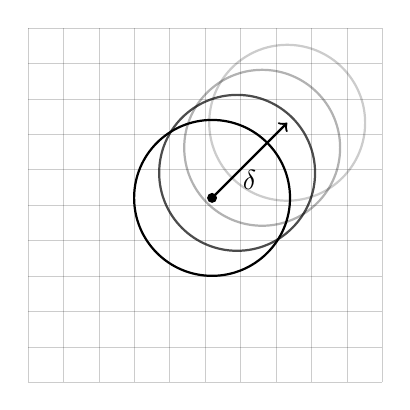
\begin{tikzpicture}[scale=0.9]

        % Domain is blue
        % \fill[blue!30] (0.1, 0.1) circle (1.5cm);

        \coordinate (p0) at (0.1, 0.1);  % the origin of the circle

        \draw[black,line width=0.8pt, opacity=1.0 ] (0.1, 0.1) circle (1.1cm);
        \draw[black,line width=0.8pt, opacity=0.7 ] (0.4535, 0.4535) circle (1.1cm);
        \draw[black,line width=0.8pt, opacity=0.3 ] (0.807, 0.807) circle (1.1cm);
        \draw[black,line width=0.8pt, opacity=0.2 ] (1.16, 1.16) circle (1.1cm);

        % Drawing points
        \fill[black] (p0) circle (2pt);
        \pgfmathsetmacro{\pOneX}{0.1 + 1.5*sqrt(2)*0.5}
        \pgfmathsetmacro{\pOneY}{0.1 + 1.5*sqrt(2)*0.5}
        \coordinate (p1) at (\pOneX, \pOneY);

        \draw[->, thick] (p0) -- (p1) node[midway,below] {$\delta$};
        % Background mesh
        \foreach \i in {-2.5, -2, ..., 2.5} {
            \draw[line width=0.1pt, shift={(-2.5,\i)}, opacity=0.2] (0,0) -- (5,0);
            \draw[line width=0.1pt, shift={(\i,-2.5)},opacity=0.2] (0,0) -- (0,5);
        }

    \end{tikzpicture}
    \caption{Illustration of several iterations of the translation test with translation distance $\delta$ from  $(0,2 \sqrt{2}h)  $. Remark that the circle is fixed in the origin, and the background mesh is translated diagonally. }
    \label{fig:illustration_translation}
\end{figure}



\begin{figure}[hpbt!]
\centering

\subfloat[]{%
% Recommended preamble:
% \usetikzlibrary{arrows.meta}
% \usetikzlibrary{backgrounds}
% \usepgfplotslibrary{patchplots}
% \usepgfplotslibrary{fillbetween}
% \pgfplotsset{%
%     layers/standard/.define layer set={%
%         background,axis background,axis grid,axis ticks,axis lines,axis tick labels,pre main,main,axis descriptions,axis foreground%
%     }{
%         grid style={/pgfplots/on layer=axis grid},%
%         tick style={/pgfplots/on layer=axis ticks},%
%         axis line style={/pgfplots/on layer=axis lines},%
%         label style={/pgfplots/on layer=axis descriptions},%
%         legend style={/pgfplots/on layer=axis descriptions},%
%         title style={/pgfplots/on layer=axis descriptions},%
%         colorbar style={/pgfplots/on layer=axis descriptions},%
%         ticklabel style={/pgfplots/on layer=axis tick labels},%
%         axis background@ style={/pgfplots/on layer=axis background},%
%         3d box foreground style={/pgfplots/on layer=axis foreground},%
%     },
% }

\begin{tikzpicture}[/tikz/background rectangle/.style={fill={rgb,1:red,1.0;green,1.0;blue,1.0}, fill opacity={1.0}, draw opacity={1.0}}, show background rectangle]
\begin{axis}[point meta max={nan}, point meta min={nan}, legend cell align={left}, legend columns={1}, title={}, title style={at={{(0.5,1)}}, anchor={south}, font={{\fontsize{14 pt}{18.2 pt}\selectfont}}, color={rgb,1:red,0.0;green,0.0;blue,0.0}, draw opacity={1.0}, rotate={0.0}, align={center}}, legend style={color={rgb,1:red,0.0;green,0.0;blue,0.0}, draw opacity={1.0}, line width={1}, solid, fill={rgb,1:red,1.0;green,1.0;blue,1.0}, fill opacity={1.0}, text opacity={1.0}, font={{\fontsize{12 pt}{15.600000000000001 pt}\selectfont}}, text={rgb,1:red,0.0;green,0.0;blue,0.0}, cells={anchor={center}}, at={(1.02, 1)}, anchor={north west}}, axis background/.style={fill={rgb,1:red,1.0;green,1.0;blue,1.0}, opacity={1.0}}, anchor={north west}, xshift={1.0mm}, yshift={-1.0mm}, width={145.4mm}, height={48.8mm}, scaled x ticks={false}, xlabel={}, x tick style={color={rgb,1:red,0.0;green,0.0;blue,0.0}, opacity={1.0}}, x tick label style={color={rgb,1:red,0.0;green,0.0;blue,0.0}, opacity={1.0}, rotate={0}}, xlabel style={at={(ticklabel cs:0.5)}, anchor=near ticklabel, at={{(ticklabel cs:0.5)}}, anchor={near ticklabel}, font={{\fontsize{11 pt}{14.3 pt}\selectfont}}, color={rgb,1:red,0.0;green,0.0;blue,0.0}, draw opacity={1.0}, rotate={0.0}}, xmajorgrids={true}, xmin={-0.014318912319027599}, xmax={0.49161598961994724}, xticklabels={{$0.0$,$0.1$,$0.2$,$0.3$,$0.4$}}, xtick={{0.0,0.1,0.2,0.30000000000000004,0.4}}, xtick align={inside}, xticklabel style={font={{\fontsize{8 pt}{10.4 pt}\selectfont}}, color={rgb,1:red,0.0;green,0.0;blue,0.0}, draw opacity={1.0}, rotate={0.0}}, x grid style={color={rgb,1:red,0.0;green,0.0;blue,0.0}, draw opacity={0.1}, line width={0.5}, solid}, axis x line*={left}, x axis line style={color={rgb,1:red,0.0;green,0.0;blue,0.0}, draw opacity={1.0}, line width={1}, solid}, scaled y ticks={false}, ylabel={}, y tick style={color={rgb,1:red,0.0;green,0.0;blue,0.0}, opacity={1.0}}, y tick label style={color={rgb,1:red,0.0;green,0.0;blue,0.0}, opacity={1.0}, rotate={0}}, ylabel style={at={(ticklabel cs:0.5)}, anchor=near ticklabel, at={{(ticklabel cs:0.5)}}, anchor={near ticklabel}, font={{\fontsize{11 pt}{14.3 pt}\selectfont}}, color={rgb,1:red,0.0;green,0.0;blue,0.0}, draw opacity={1.0}, rotate={0.0}}, ymode={log}, log basis y={10}, ymajorgrids={true}, ymin={0.21057015125625464}, ymax={1.6984113670504998e23}, yticklabels={{$10^{0}$,$10^{5}$,$10^{10}$,$10^{15}$,$10^{20}$}}, ytick={{1.0,100000.0,1.0e10,1.0e15,1.0e20}}, ytick align={inside}, yticklabel style={font={{\fontsize{8 pt}{10.4 pt}\selectfont}}, color={rgb,1:red,0.0;green,0.0;blue,0.0}, draw opacity={1.0}, rotate={0.0}}, y grid style={color={rgb,1:red,0.0;green,0.0;blue,0.0}, draw opacity={0.1}, line width={0.5}, solid}, axis y line*={left}, y axis line style={color={rgb,1:red,0.0;green,0.0;blue,0.0}, draw opacity={1.0}, line width={1}, solid}, colorbar={false}]
    [\addlegendimage{empty legend}] \addlegendentry[font={{\fontsize{11 pt}{14.3 pt}\selectfont}}, text={rgb,1:red,0.0;green,0.0;blue,0.0}] {\hspace{-.6cm}{\textbf{$(\gamma, \gamma_1, \gamma_2)$}}}
    \addplot[color={rgb,1:red,0.0;green,0.0;blue,1.0}, name path={121f4aba-f4f6-4058-9c2e-b56e02e7657b}, draw opacity={1.0}, line width={1}, solid]
        table[row sep={\\}]
        {
            \\
            0.0  1.0179555234550795e6  \\
            0.0009565071689397187  1.0181257149508498e6  \\
            0.0019130143378794373  1.0182953659619611e6  \\
            0.002869521506819156  1.0184644734707349e6  \\
            0.0038260286757588746  1.0186330347316939e6  \\
            0.004782535844698593  1.0188010469947746e6  \\
            0.005739043013638312  1.0189685084522819e6  \\
            0.0066955501825780315  1.0191354177615213e6  \\
            0.007652057351517749  1.0193017739982733e6  \\
            0.008608564520457468  1.0194675775380677e6  \\
            0.009565071689397187  1.0196328288666179e6  \\
            0.010521578858336907  1.0197975303232376e6  \\
            0.011478086027276624  1.0199616846673312e6  \\
            0.012434593196216343  1.0201252962091755e6  \\
            0.013391100365156063  1.0202883709901893e6  \\
            0.01434760753409578  1.0204509151955257e6  \\
            0.015304114703035498  1.0206129383146905e6  \\
            0.016260621871975217  1.0207744501496791e6  \\
            0.017217129040914936  1.2091451665733533e6  \\
            0.018173636209854658  1.233597888415578e6  \\
            0.019130143378794373  1.2330888905457777e6  \\
            0.020086650547734092  1.2324507469448263e6  \\
            0.021043157716673814  1.2316845453848245e6  \\
            0.02199966488561353  1.230791150526075e6  \\
            0.022956172054553248  1.2297711619134818e6  \\
            0.02391267922349297  1.2286249693590365e6  \\
            0.024869186392432685  1.227352822856193e6  \\
            0.025825693561372404  1.2259548775048105e6  \\
            0.026782200730312126  1.2244312088972682e6  \\
            0.027738707899251844  1.2227817971026548e6  \\
            0.02869521506819156  1.221006486368886e6  \\
            0.02965172223713128  1.2191049550959668e6  \\
            0.030608229406070997  1.223260041811732e6  \\
            0.031564736575010716  1.2283735094325568e6  \\
            0.032521243743950434  1.2305946045916907e6  \\
            0.03347775091289015  1.2212074257740362e6  \\
            0.03443425808182987  1.2186623348770197e6  \\
            0.0353907652507696  1.2159907185558877e6  \\
            0.036347272419709316  1.213476329261407e6  \\
            0.03730377958864903  1.2180422646496962e6  \\
            0.038260286757588746  1.2222074864412204e6  \\
            0.039216793926528465  1.225927358049082e6  \\
            0.040173301095468184  1.2291910099634835e6  \\
            0.04112980826440791  1.2319909005285734e6  \\
            0.04208631543334763  1.2343224099487942e6  \\
            0.043042822602287346  1.2361834535837958e6  \\
            0.04399932977122706  1.2375741080208344e6  \\
            0.04495583694016678  1.2384962569015154e6  \\
            0.045912344109106495  1.2363580091486534e6  \\
            0.046868851278046214  1.2455092040773167e6  \\
            0.04782535844698594  1.245101591334316e6  \\
            0.04878186561592566  1.2445898095865883e6  \\
            0.04973837278486537  1.2439945036676747e6  \\
            0.05069487995380509  1.243297885566909e6  \\
            0.05165138712274481  1.2424975745624856e6  \\
            0.052607894291684526  1.2416034713857034e6  \\
            0.05356440146062425  1.2406059234081847e6  \\
            0.05452090862956397  1.2395039783482004e6  \\
            0.05547741579850369  1.2383038372359064e6  \\
            0.0564339229674434  1.237002395574417e6  \\
            0.05739043013638312  1.2356061461135934e6  \\
            0.05834693730532284  1.2341041040119084e6  \\
            0.05930344447426256  1.2360406791482184e6  \\
            0.060259951643202275  1.235865040319504e6  \\
            0.061216458812141994  1.2356731715361667e6  \\
            0.06217296598108171  1.2354648450339446e6  \\
            0.06312947315002143  1.2352398471191232e6  \\
            0.06408598031896115  1.234997982345449e6  \\
            0.06504248748790087  1.234762503651092e6  \\
            0.06599899465684059  1.2345222466579112e6  \\
            0.0669555018257803  1.2342690071343563e6  \\
            0.06791200899472002  1.234009284085122e6  \\
            0.06886851616365974  1.233733319401992e6  \\
            0.06982502333259948  1.233453868158291e6  \\
            0.0707815305015392  1.2331794730052396e6  \\
            0.07173803767047891  1.2328893973462922e6  \\
            0.07269454483941863  1.2326259279347644e6  \\
            0.07365105200835834  1.233157336928129e6  \\
            0.07460755917729806  1.23386088274286e6  \\
            0.07556406634623777  1.234169708850581e6  \\
            0.07652057351517749  1.242858455624462e6  \\
            0.07747708068411721  1.2431567479870366e6  \\
            0.07843358785305693  1.2433453075211125e6  \\
            0.07939009502199665  1.243423739956339e6  \\
            0.08034660219093637  1.243391413262701e6  \\
            0.08130310935987609  1.2510733210976645e6  \\
            0.08225961652881582  1.2504395501612767e6  \\
            0.08321612369775554  1.2497835665882882e6  \\
            0.08417263086669526  1.2491050266723577e6  \\
            0.08512913803563497  1.2484035858534882e6  \\
            0.08608564520457469  1.2476788981418824e6  \\
            0.0870421523735144  1.246930615973239e6  \\
            0.08799865954245412  1.2461583916301732e6  \\
            0.08895516671139383  1.2453618769608436e6  \\
            0.08991167388033355  1.2445407235453392e6  \\
            0.09086818104927327  1.2436945833392632e6  \\
            0.09182468821821299  1.2428231091853755e6  \\
            0.09278119538715271  1.241925955259275e6  \\
            0.09373770255609243  1.241002776399994e6  \\
            0.09469420972503216  1.2400532305577202e6  \\
            0.09565071689397188  1.2390769774743658e6  \\
            0.0966072240629116  1.2380736794564845e6  \\
            0.09756373123185132  1.237043002117442e6  \\
            0.09852023840079104  1.2465768765525008e6  \\
            0.09947674556973074  1.2462657012467424e6  \\
            0.10043325273867046  1.2457605261542615e6  \\
            0.10138975990761018  1.2450651694851227e6  \\
            0.1023462670765499  1.2441830167211408e6  \\
            0.10330277424548961  1.2431170909697714e6  \\
            0.10425928141442933  1.241870119875073e6  \\
            0.10521578858336905  1.2404445980974098e6  \\
            0.10617229575230877  1.2388428426283998e6  \\
            0.1071288029212485  1.237067045927614e6  \\
            0.10808531009018822  1.2351193225701228e6  \\
            0.10904181725912794  1.2330017537354673e6  \\
            0.10999832442806766  1.2307164252952877e6  \\
            0.11095483159700738  1.2282654659512546e6  \\
            0.1119113387659471  1.2256510771402407e6  \\
            0.1128678459348868  1.222875563279963e6  \\
            0.11382435310382652  1.2199413572640864e6  \\
            0.11478086027276624  1.216851042502871e6  \\
            0.11573736744170596  1.213607373347309e6  \\
            0.11669387461064568  1.2102132916393583e6  \\
            0.1176503817795854  1.2067609265648907e6  \\
            0.11860688894852511  1.203194826498756e6  \\
            0.11956339611746483  1.2013548330849437e6  \\
            0.12051990328640455  1.2049969994016944e6  \\
            0.12147641045534427  1.2084862174315345e6  \\
            0.12243291762428399  1.2119289438706622e6  \\
            0.1233894247932237  1.2152481994506025e6  \\
            0.12434593196216343  1.218415547222522e6  \\
            0.12530243913110314  1.221428140564509e6  \\
            0.12625894630004286  1.2242833137640064e6  \\
            0.12721545346898258  1.226978560425655e6  \\
            0.1281719606379223  1.2295115156027097e6  \\
            0.12912846780686202  1.231879929439329e6  \\
            0.13008497497580174  1.2340816404139986e6  \\
            0.13104148214474146  1.2361145462051043e6  \\
            0.13199798931368117  1.237976567524563e6  \\
            0.1329544964826209  1.2396656118621991e6  \\
            0.1339110036515606  1.241179530987284e6  \\
            0.13486751082050033  1.2425160768806222e6  \\
            0.13582401798944005  1.2436728503125946e6  \\
            0.13678052515837977  1.2446472476319035e6  \\
            0.1377370323273195  1.2454364012197815e6  \\
            0.13869353949625923  1.2460371154729426e6  \\
            0.13965004666519895  1.2464457980415442e6  \\
            0.14060655383413867  1.236517293631431e6  \\
            0.1415630610030784  1.2375617845980416e6  \\
            0.1425195681720181  1.2385787306901962e6  \\
            0.14347607534095783  1.2395684643607e6  \\
            0.14443258250989754  1.2405313212932243e6  \\
            0.14538908967883726  1.2414676409411442e6  \\
            0.14634559684777695  1.2423777643449355e6  \\
            0.14730210401671667  1.243262035454236e6  \\
            0.1482586111856564  1.2441207991429928e6  \\
            0.1492151183545961  1.2449544024232496e6  \\
            0.15017162552353583  1.2457631928722856e6  \\
            0.15112813269247555  1.246547518766125e6  \\
            0.15208463986141527  1.2473077286300762e6  \\
            0.15304114703035498  1.2480441701166248e6  \\
            0.1539976541992947  1.2487571911075888e6  \\
            0.15495416136823442  1.2494471381745494e6  \\
            0.15591066853717414  1.2501143569978832e6  \\
            0.15686717570611386  1.2507591914810883e6  \\
            0.15782368287505358  1.2433334439461522e6  \\
            0.1587801900439933  1.2434214695052078e6  \\
            0.15973669721293302  1.243398321802335e6  \\
            0.16069320438187273  1.2432647625024477e6  \\
            0.16164971155081245  1.2430213007856184e6  \\
            0.16260621871975217  1.2426682237624717e6  \\
            0.16356272588869192  1.2340656067885766e6  \\
            0.16451923305763164  1.2335574899477765e6  \\
            0.16547574022657136  1.232662271169399e6  \\
            0.16643224739551107  1.232752783140874e6  \\
            0.1673887545644508  1.2330366911146052e6  \\
            0.1683452617333905  1.233317775749177e6  \\
            0.16930176890233023  1.2335957787188618e6  \\
            0.17025827607126995  1.2338730182258852e6  \\
            0.17121478324020967  1.234141270203603e6  \\
            0.17217129040914939  1.2343958821629102e6  \\
            0.17312779757808908  1.2346444441110475e6  \\
            0.1740843047470288  1.2348795814122215e6  \\
            0.1750408119159685  1.23512103450606e6  \\
            0.17599731908490823  1.2353544429064486e6  \\
            0.17695382625384795  1.2355710791896114e6  \\
            0.17791033342278767  1.2357711491822815e6  \\
            0.1788668405917274  1.2359548739529208e6  \\
            0.1798233477606671  1.2333158973744188e6  \\
            0.18077985492960683  1.234868538258127e6  \\
            0.18173636209854654  1.2363170282884045e6  \\
            0.18269286926748626  1.2376663498850022e6  \\
            0.18364937643642598  1.2389149479336585e6  \\
            0.1846058836053657  1.240068034292378e6  \\
            0.18556239077430542  1.2411177180159711e6  \\
            0.18651889794324514  1.2420632425889457e6  \\
            0.18747540511218486  1.2429107025161437e6  \\
            0.18843191228112458  1.243659150911169e6  \\
            0.18938841945006432  1.2443039494620063e6  \\
            0.19034492661900404  1.2448586955143237e6  \\
            0.19130143378794376  1.245318451987207e6  \\
            0.19225794095688348  1.2362391568447775e6  \\
            0.1932144481258232  1.2364683538809856e6  \\
            0.19417095529476291  1.2380935659856782e6  \\
            0.19512746246370263  1.2369374991313473e6  \\
            0.19608396963264235  1.2353117810575613e6  \\
            0.19704047680158207  1.2332153871774112e6  \\
            0.1979969839705218  1.2306492772933058e6  \\
            0.19895349113946148  1.2276167547953266e6  \\
            0.1999099983084012  1.2241238517951735e6  \\
            0.20086650547734092  1.2201797224064474e6  \\
            0.20182301264628064  1.215797053733971e6  \\
            0.20277951981522035  1.2146075828201193e6  \\
            0.20373602698416007  1.217342322324909e6  \\
            0.2046925341530998  1.2199507171906303e6  \\
            0.2056490413220395  1.2224324377199705e6  \\
            0.20660554849097923  1.2298769852690059e6  \\
            0.20756205565991895  1.2261468851203783e6  \\
            0.20851856282885867  1.2197759321210487e6  \\
            0.20947506999779839  1.2200715257232226e6  \\
            0.2104315771667381  1.2219098965753252e6  \\
            0.21138808433567782  1.2236222283176822e6  \\
            0.21234459150461754  1.2252087587487653e6  \\
            0.21330109867355726  1.2266695696690683e6  \\
            0.214257605842497  1.2280046301398978e6  \\
            0.21521411301143673  1.229213824301008e6  \\
            0.21617062018037644  1.230296953400483e6  \\
            0.21712712734931616  1.2312537055565142e6  \\
            0.21808363451825588  1.2320835944793522e6  \\
            0.2190401416871956  1.2327858920073041e6  \\
            0.21999664885613532  1.2333596044649594e6  \\
            0.22095315602507504  1.2090961459801274e6  \\
            0.22190966319401476  1.209161502008475e6  \\
            0.22286617036295447  1.0206937574452658e6  \\
            0.2238226775318942  1.0205319914513119e6  \\
            0.2247791847008339  1.0203697089101315e6  \\
            0.2257356918697736  1.0202069002863431e6  \\
            0.22669219903871332  1.0200435579128822e6  \\
            0.22764870620765304  1.0198796755012079e6  \\
            0.22860521337659276  1.0197152480102839e6  \\
            0.22956172054553248  1.0195502720980027e6  \\
            0.2305182277144722  1.0193847447509527e6  \\
            0.23147473488341191  1.0192186649607703e6  \\
            0.23243124205235163  1.0190520321875904e6  \\
            0.23338774922129135  1.0188848466070251e6  \\
            0.23434425639023107  1.0187171094436576e6  \\
            0.2353007635591708  1.0185488225210063e6  \\
            0.2362572707281105  1.0183799878088138e6  \\
            0.23721377789705023  1.0182106082767271e6  \\
            0.23817028506598995  1.018040686462245e6  \\
            0.23912679223492966  1.0180406864685785e6  \\
            0.24008329940386938  1.018210608339077e6  \\
            0.2410398065728091  1.0183799879118683e6  \\
            0.24199631374174882  1.0185488225805977e6  \\
            0.24295282091068854  1.0187171093610384e6  \\
            0.24390932807962826  1.018884846587272e6  \\
            0.24486583524856798  1.0190520321843115e6  \\
            0.2458223424175077  1.0192186649803116e6  \\
            0.2467788495864474  1.019384744772071e6  \\
            0.24773535675538713  1.0195502719409815e6  \\
            0.24869186392432685  1.0197152480415311e6  \\
            0.24964837109326657  1.019879675559593e6  \\
            0.2506048782622063  1.0200435579868616e6  \\
            0.25156138543114603  1.0202069003053923e6  \\
            0.2525178926000857  1.0203697087620262e6  \\
            0.25347439976902547  1.0205319911823719e6  \\
            0.25443090693796516  1.0206937573752184e6  \\
            0.2553874141069049  1.2091615005293e6  \\
            0.2563439212758446  1.2090961447127059e6  \\
            0.25730042844478435  1.2333596029483122e6  \\
            0.25825693561372404  1.2327858903403664e6  \\
            0.2592134427826638  1.2320835929818687e6  \\
            0.2601699499516035  1.2312537039720032e6  \\
            0.2611264571205432  1.2302969519464811e6  \\
            0.2620829642894829  1.2292138228508085e6  \\
            0.26303947145842266  1.2280046288799676e6  \\
            0.26399597862736235  1.2266695684906254e6  \\
            0.2649524857963021  1.2252087570975001e6  \\
            0.2659089929652418  1.2236222266530828e6  \\
            0.26686550013418153  1.2219098950911015e6  \\
            0.2678220073031212  1.2200715243329008e6  \\
            0.26877851447206097  1.2197759337953662e6  \\
            0.26973502164100066  1.2261468866185572e6  \\
            0.2706915288099404  1.2298769865646097e6  \\
            0.2716480359788801  1.2224324362343561e6  \\
            0.27260454314781984  1.219950715605558e6  \\
            0.27356105031675954  1.2173423207991538e6  \\
            0.2745175574856993  1.2146075814764604e6  \\
            0.275474064654639  1.21579705513671e6  \\
            0.2764305718235787  1.2201797235765506e6  \\
            0.27738707899251847  1.2241238529774135e6  \\
            0.27834358616145816  1.22761675589912e6  \\
            0.2793000933303979  1.2306492779918606e6  \\
            0.2802566004993376  1.2332153881256562e6  \\
            0.28121310766827734  1.235311781576566e6  \\
            0.28216961483721703  1.236937499775045e6  \\
            0.2831261220061568  1.2380935664565426e6  \\
            0.28408262917509647  1.236468352624863e6  \\
            0.2850391363440362  1.2362391568319688e6  \\
            0.2859956435129759  1.2453184501229392e6  \\
            0.28695215068191565  1.2448586938537853e6  \\
            0.28790865785085534  1.2443039481058214e6  \\
            0.2888651650197951  1.2436591494233678e6  \\
            0.2898216721887348  1.242910700848454e6  \\
            0.2907781793576745  1.2420632408159215e6  \\
            0.29173468652661416  1.2411177164404916e6  \\
            0.2926911936955539  1.2400680327355373e6  \\
            0.2936477008644936  1.2389149460645828e6  \\
            0.29460420803343335  1.23766634837391e6  \\
            0.29556071520237304  1.236317026652085e6  \\
            0.2965172223713128  1.2348685366306093e6  \\
            0.2974737295402525  1.2333158955906462e6  \\
            0.2984302367091922  1.235954873876909e6  \\
            0.2993867438781319  1.2357711491128732e6  \\
            0.30034325104707166  1.23557107931495e6  \\
            0.3012997582160114  1.2353544427905055e6  \\
            0.3022562653849511  1.2351210344050392e6  \\
            0.30321277255389084  1.2348795812820804e6  \\
            0.30416927972283053  1.234644444009843e6  \\
            0.3051257868917703  1.2343958822202806e6  \\
            0.30608229406070997  1.2341412697733021e6  \\
            0.3070388012296497  1.2338730181599066e6  \\
            0.3079953083985894  1.23359577851411e6  \\
            0.30895181556752915  1.2333177755050624e6  \\
            0.30990832273646884  1.2330366906366255e6  \\
            0.3108648299054086  1.2327527825754902e6  \\
            0.3118213370743483  1.2326622725753812e6  \\
            0.31277784424328803  1.2335574912308706e6  \\
            0.3137343514122277  1.2340656083240139e6  \\
            0.31469085858116747  1.242668225131712e6  \\
            0.31564736575010716  1.2430213023625973e6  \\
            0.3166038729190469  1.243264763572573e6  \\
            0.3175603800879866  1.2433983234064474e6  \\
            0.31851688725692634  1.2434214711188367e6  \\
            0.31947339442586603  1.2433334453012536e6  \\
            0.3204299015948058  1.2507591909849248e6  \\
            0.32138640876374547  1.2501143565039348e6  \\
            0.3223429159326852  1.2494471374889982e6  \\
            0.3232994231016249  1.248757190440982e6  \\
            0.32425593027056465  1.248044169387709e6  \\
            0.32521243743950434  1.2473077279028427e6  \\
            0.3261689446084441  1.2465475184446438e6  \\
            0.32712545177738384  1.245763192460483e6  \\
            0.3280819589463235  1.244954401927941e6  \\
            0.3290384661152633  1.2441207985952403e6  \\
            0.32999497328420296  1.2432620346726493e6  \\
            0.3309514804531427  1.2423777637575273e6  \\
            0.3319079876220824  1.2414676401976154e6  \\
            0.33286449479102215  1.2405313208734319e6  \\
            0.33382100195996184  1.2395684636583375e6  \\
            0.3347775091289016  1.2385787300390631e6  \\
            0.3357340162978413  1.237561783994126e6  \\
            0.336690523466781  1.236517292663488e6  \\
            0.3376470306357207  1.2464457965037029e6  \\
            0.33860353780466046  1.2460371136164058e6  \\
            0.33956004497360015  1.2454363994267248e6  \\
            0.3405165521425399  1.2446472462546807e6  \\
            0.3414730593114796  1.2436728488184689e6  \\
            0.34242956648041933  1.242516075423309e6  \\
            0.343386073649359  1.241179529462511e6  \\
            0.34434258081829877  1.239665610346928e6  \\
            0.3452990879872384  1.2379765659521576e6  \\
            0.34625559515617815  1.236114544841827e6  \\
            0.34721210232511784  1.2340816389263752e6  \\
            0.3481686094940576  1.2318799278810136e6  \\
            0.3491251166629973  1.2295115141140819e6  \\
            0.350081623831937  1.226978558955212e6  \\
            0.3510381310008768  1.2242833120374104e6  \\
            0.35199463816981647  1.221428139124111e6  \\
            0.3529511453387562  1.2184155455997086e6  \\
            0.3539076525076959  1.2152481977149993e6  \\
            0.35486415967663565  1.2119289423312848e6  \\
            0.35582066684557534  1.2084862159224746e6  \\
            0.3567771740145151  1.2049969976990253e6  \\
            0.3577336811834548  1.2013548313908277e6  \\
            0.3586901883523945  1.2031948280255063e6  \\
            0.3596466955213342  1.2067609279225785e6  \\
            0.36060320269027396  1.21021329310911e6  \\
            0.36155970985921365  1.2136073746786208e6  \\
            0.3625162170281534  1.2168510440183636e6  \\
            0.3634727241970931  1.2199413586777693e6  \\
            0.36442923136603284  1.2228755647973393e6  \\
            0.3653857385349725  1.225651078596844e6  \\
            0.3663422457039123  1.2282654675389433e6  \\
            0.36729875287285196  1.2307164269870415e6  \\
            0.3682552600417917  1.2330017550584967e6  \\
            0.3692117672107314  1.2351193240506616e6  \\
            0.37016827437967115  1.2370670475362819e6  \\
            0.37112478154861084  1.2388428442495929e6  \\
            0.3720812887175506  1.2404445996392455e6  \\
            0.3730377958864903  1.2418701212271731e6  \\
            0.37399430305543  1.2431170925939525e6  \\
            0.3749508102243697  1.2441830180759726e6  \\
            0.37590731739330946  1.2450651710638313e6  \\
            0.37686382456224915  1.2457605275652702e6  \\
            0.3778203317311889  1.2462657025240401e6  \\
            0.37877683890012864  1.2465768781858115e6  \\
            0.37973334606906833  1.237043003136531e6  \\
            0.3806898532380081  1.2380736802030266e6  \\
            0.38164636040694777  1.2390769781462809e6  \\
            0.3826028675758875  1.2400532313382125e6  \\
            0.3835593747448272  1.2410027771592392e6  \\
            0.38451588191376695  1.2419259556616584e6  \\
            0.38547238908270665  1.2428231098281252e6  \\
            0.3864288962516464  1.2436945839115249e6  \\
            0.3873854034205861  1.2445407240422454e6  \\
            0.38834191058952583  1.245361877578498e6  \\
            0.3892984177584655  1.246158392030675e6  \\
            0.39025492492740527  1.246930616488234e6  \\
            0.39121143209634496  1.2476788986599518e6  \\
            0.3921679392652847  1.248403586370587e6  \\
            0.3931244464342244  1.2491050272994514e6  \\
            0.39408095360316414  1.249783566954197e6  \\
            0.39503746077210383  1.250439550592568e6  \\
            0.3959939679410436  1.2510733214590065e6  \\
            0.39695047510998327  1.2433914117992052e6  \\
            0.39790698227892296  1.2434237384030754e6  \\
            0.39886348944786265  1.2433453061688235e6  \\
            0.3998199966168024  1.2431567464361743e6  \\
            0.4007765037857421  1.242858454334037e6  \\
            0.40173301095468184  1.2341697073355457e6  \\
            0.4026895181236216  1.2338608809769852e6  \\
            0.4036460252925613  1.2331573352990195e6  \\
            0.404602532461501  1.232625928322924e6  \\
            0.4055590396304407  1.2328893977195255e6  \\
            0.40651554679938046  1.2331794730238973e6  \\
            0.40747205396832015  1.2334538683050196e6  \\
            0.4084285611372599  1.2337333191143216e6  \\
            0.4093850683061996  1.2340092840065164e6  \\
            0.41034157547513933  1.2342690070990333e6  \\
            0.411298082644079  1.2345222467035253e6  \\
            0.41225458981301877  1.2347625035701e6  \\
            0.41321109698195846  1.2349979821929464e6  \\
            0.4141676041508982  1.2352398471989334e6  \\
            0.4151241113198379  1.2354648450442925e6  \\
            0.41608061848877764  1.2356731715486613e6  \\
            0.41703712565771733  1.235865040526294e6  \\
            0.4179936328266571  1.236040679165681e6  \\
            0.41895013999559677  1.2341041054555424e6  \\
            0.4199066471645365  1.235606147493869e6  \\
            0.4208631543334762  1.2370023968140092e6  \\
            0.42181966150241595  1.2383038384259103e6  \\
            0.42277616867135565  1.2395039799289985e6  \\
            0.4237326758402954  1.2406059251119052e6  \\
            0.4246891830092351  1.241603472774632e6  \\
            0.42564569017817483  1.2424975758831552e6  \\
            0.4266021973471145  1.2432978871542565e6  \\
            0.42755870451605427  1.2439945048691959e6  \\
            0.428515211684994  1.244589811189184e6  \\
            0.4294717188539337  1.245101593016431e6  \\
            0.43042822602287345  1.2455092055650156e6  \\
            0.43138473319181314  1.2363580104589767e6  \\
            0.4323412403607529  1.238496256396463e6  \\
            0.4332977475296926  1.2375741072871827e6  \\
            0.4342542546986323  1.236183452629329e6  \\
            0.435210761867572  1.2343224092380665e6  \\
            0.43616726903651176  1.2319908996172352e6  \\
            0.43712377620545145  1.229191008857343e6  \\
            0.4380802833743912  1.2259273564957436e6  \\
            0.4390367905433309  1.2222074848879352e6  \\
            0.43999329771227064  1.2180422632199232e6  \\
            0.4409498048812103  1.2134763275539882e6  \\
            0.4419063120501501  1.2159907199667285e6  \\
            0.44286281921908976  1.2186623362688855e6  \\
            0.4438193263880295  1.2212074271615513e6  \\
            0.4447758335569692  1.2305946030385923e6  \\
            0.44573234072590895  1.2283735081169389e6  \\
            0.44668884789484864  1.223260040002224e6  \\
            0.4476453550637884  1.2191049566289838e6  \\
            0.4486018622327281  1.2210064876200648e6  \\
            0.4495583694016678  1.2227817983135488e6  \\
            0.4505148765706075  1.224431210239863e6  \\
            0.4514713837395472  1.2259548790262889e6  \\
            0.45242789090848695  1.2273528241346767e6  \\
            0.45338439807742664  1.228624970853593e6  \\
            0.4543409052463664  1.2297711634259156e6  \\
            0.4552974124153061  1.2307911519967804e6  \\
            0.4562539195842458  1.2316845470410981e6  \\
            0.4572104267531855  1.232450748487027e6  \\
            0.45816693392212526  1.2330888919318886e6  \\
            0.45912344109106495  1.2335978898180572e6  \\
            0.4600799482600047  1.209145168022004e6  \\
            0.4610364554289444  1.0207744502766905e6  \\
            0.46199296259788414  1.0206129382258954e6  \\
            0.46294946976682383  1.0204509152519604e6  \\
            0.4639059769357636  1.0202883708546273e6  \\
            0.46486248410470327  1.0201252963143656e6  \\
            0.465818991273643  1.0199616844715854e6  \\
            0.4667754984425827  1.0197975301918593e6  \\
            0.46773200561152245  1.0196328288150667e6  \\
            0.46868851278046214  1.0194675773483972e6  \\
            0.4696450199494019  1.0193017738625795e6  \\
            0.4706015271183416  1.0191354177796005e6  \\
            0.4715580342872813  1.0189685084720682e6  \\
            0.472514541456221  1.0188010468909182e6  \\
            0.47347104862516076  1.0186330345355462e6  \\
            0.47442755579410045  1.0184644733241638e6  \\
            0.4753840629630402  1.0182953659889288e6  \\
            0.4763405701319799  1.0181257149344576e6  \\
            0.47729707730091964  1.0179555234684236e6  \\
        }
        ;
    \addlegendentry {$(20, 10, 1) $}
    \addplot[color={rgb,1:red,1.0;green,0.0;blue,0.0}, name path={795f6fd8-7de7-4120-8a65-1c5a7c3bb18f}, draw opacity={1.0}, line width={1}, solid]
        table[row sep={\\}]
        {
            \\
            0.0  3.721357938320085e8  \\
            0.0009565071689397187  5.756153750461564e8  \\
            0.0019130143378794373  9.094431381902353e8  \\
            0.002869521506819156  1.4729612821583197e9  \\
            0.0038260286757588746  2.455938195068614e9  \\
            0.004782535844698593  4.236983650940315e9  \\
            0.005739043013638312  7.610921858518547e9  \\
            0.0066955501825780315  1.4348547158850521e10  \\
            0.007652057351517749  2.8685227767746593e10  \\
            0.008608564520457468  6.163232945157956e10  \\
            0.009565071689397187  1.4508805864312006e11  \\
            0.010521578858336907  3.8451047397821185e11  \\
            0.011478086027276624  1.1956520467840347e12  \\
            0.012434593196216343  4.66686587427861e12  \\
            0.013391100365156063  2.582471965253527e13  \\
            0.01434760753409578  2.619061006086155e14  \\
            0.015304114703035498  1.0001874118223862e16  \\
            0.016260621871975217  1.4799028941200435e20  \\
            0.017217129040914936  3.263844584500708e9  \\
            0.018173636209854658  1.2345523391059658e15  \\
            0.019130143378794373  1.4787621142834646e12  \\
            0.020086650547734092  8.385090413768022e10  \\
            0.021043157716673814  1.284327114640879e10  \\
            0.02199966488561353  6.924451050202312e9  \\
            0.022956172054553248  8.172620809808402e9  \\
            0.02391267922349297  9.688872060649523e9  \\
            0.024869186392432685  1.1540553998559074e10  \\
            0.025825693561372404  1.3814603744854113e10  \\
            0.026782200730312126  1.6623948680013752e10  \\
            0.027738707899251844  2.011645593237398e10  \\
            0.02869521506819156  2.4487276663075974e10  \\
            0.02965172223713128  2.9996160515280262e10  \\
            0.030608229406070997  3.69919698657115e10  \\
            0.031564736575010716  4.594778213458608e10  \\
            0.032521243743950434  5.751172809866871e10  \\
            0.03347775091289015  3.0004174801782655e15  \\
            0.03443425808182987  2.3436733949341902e13  \\
            0.0353907652507696  1.8062641778356182e12  \\
            0.036347272419709316  3.15543892015384e11  \\
            0.03730377958864903  2.0131809005630545e11  \\
            0.038260286757588746  2.6768126909493558e11  \\
            0.039216793926528465  3.6070527251151263e11  \\
            0.040173301095468184  9.019842701339285e11  \\
            0.04112980826440791  3.2353096048658345e12  \\
            0.04208631543334763  1.581133900111568e13  \\
            0.043042822602287346  1.3019083368160038e14  \\
            0.04399932977122706  3.142786952894669e15  \\
            0.04495583694016678  3.152561161281024e18  \\
            0.045912344109106495  4.886072771663222e12  \\
            0.046868851278046214  3.5763473845516742e22  \\
            0.04782535844698594  1.4648537476872278e16  \\
            0.04878186561592566  3.404881963293056e14  \\
            0.04973837278486537  4.214640762017944e13  \\
            0.05069487995380509  8.290575190347425e13  \\
            0.05165138712274481  1.7656994559391847e14  \\
            0.052607894291684526  4.1581936623035556e14  \\
            0.05356440146062425  1.1166668318931459e15  \\
            0.05452090862956397  3.586500200680247e15  \\
            0.05547741579850369  1.4920071800820578e16  \\
            0.0564339229674434  9.335841667035197e16  \\
            0.05739043013638312  1.2308871131708065e18  \\
            0.05834693730532284  1.0225612620134683e20  \\
            0.05930344447426256  2.6336348454869373e10  \\
            0.060259951643202275  2.134412895665461e10  \\
            0.061216458812141994  1.9036574540139565e10  \\
            0.06217296598108171  2.0013127618390774e10  \\
            0.06312947315002143  3.9361323766369896e10  \\
            0.06408598031896115  8.487773361438525e9  \\
            0.06504248748790087  4.527030426368828e10  \\
            0.06599899465684059  7.322838513936945e9  \\
            0.0669555018257803  3.196877008089777e9  \\
            0.06791200899472002  1.7210347376629534e9  \\
            0.06886851616365974  1.0237440439494371e9  \\
            0.06982502333259948  6.472984584716145e8  \\
            0.0707815305015392  4.269971070240713e8  \\
            0.07173803767047891  2.90759190442263e8  \\
            0.07269454483941863  2.0300490796562397e8  \\
            0.07365105200835834  1.446549966958421e8  \\
            0.07460755917729806  1.0484949955290213e8  \\
            0.07556406634623777  7.71120546249345e7  \\
            0.07652057351517749  7.694424253764698e16  \\
            0.07747708068411721  4.661921484729405e14  \\
            0.07843358785305693  3.644403798494565e13  \\
            0.07939009502199665  7.064838068197242e12  \\
            0.08034660219093637  2.2646380859776196e12  \\
            0.08130310935987609  1.4543427242065215e20  \\
            0.08225961652881582  8.644134779087028e15  \\
            0.08321612369775554  2.3408961336336656e14  \\
            0.08417263086669526  2.3830535992390773e13  \\
            0.08512913803563497  4.420984712452577e12  \\
            0.08608564520457469  1.1573323530110737e12  \\
            0.0870421523735144  3.789573727689608e11  \\
            0.08799865954245412  1.4520940501977792e11  \\
            0.08895516671139383  6.25177792529281e10  \\
            0.08991167388033355  3.5943318707519905e10  \\
            0.09086818104927327  8.282114612724013e10  \\
            0.09182468821821299  2.126583216365938e11  \\
            0.09278119538715271  6.302716634232109e11  \\
            0.09373770255609243  2.278757046607296e12  \\
            0.09469420972503216  1.1046477811759746e13  \\
            0.09565071689397188  8.616966546892222e13  \\
            0.0966072240629116  1.6667211331340022e15  \\
            0.09756373123185132  4.040204175462079e17  \\
            0.09852023840079104  2.7269745069093287e8  \\
            0.09947674556973074  1.834986589373262e8  \\
            0.10043325273867046  1.250275542885058e8  \\
            0.10138975990761018  8.603677693130009e7  \\
            0.1023462670765499  5.963584152742638e7  \\
            0.10330277424548961  4.151304231053679e7  \\
            0.10425928141442933  2.8917842637567773e7  \\
            0.10521578858336905  2.0064498224887207e7  \\
            0.10617229575230877  1.3774693208077863e7  \\
            0.1071288029212485  1.161422873612523e7  \\
            0.10808531009018822  1.2654822415619396e7  \\
            0.10904181725912794  1.3937472879542679e7  \\
            0.10999832442806766  1.5859309651641303e8  \\
            0.11095483159700738  1.7348858605396435e7  \\
            0.1119113387659471  1.9715125199255772e7  \\
            0.1128678459348868  2.2913980567394286e7  \\
            0.11382435310382652  2.739517225275401e7  \\
            0.11478086027276624  3.4090590327431306e7  \\
            0.11573736744170596  4.514013779027676e7  \\
            0.11669387461064568  6.674924674798395e7  \\
            0.1176503817795854  1.2673838499076112e8  \\
            0.11860688894852511  8.66394453294898e8  \\
            0.11956339611746483  5.669462467484614e8  \\
            0.12051990328640455  2.2500507226649916e8  \\
            0.12147641045534427  8.760368939876011e7  \\
            0.12243291762428399  5.386276303172208e7  \\
            0.1233894247932237  3.8844482777763754e7  \\
            0.12434593196216343  3.037600032805295e7  \\
            0.12530243913110314  2.495180344377065e7  \\
            0.12625894630004286  2.1190018665224135e7  \\
            0.12721545346898258  1.8443785866461027e7  \\
            0.1281719606379223  1.6448357179160444e7  \\
            0.12912846780686202  2.1839488540697455e7  \\
            0.13008497497580174  1.3257003796758462e7  \\
            0.13104148214474146  1.211050706014785e7  \\
            0.13199798931368117  1.1333353054204935e7  \\
            0.1329544964826209  1.665570677106724e7  \\
            0.1339110036515606  2.4108252090164047e7  \\
            0.13486751082050033  3.465366465252125e7  \\
            0.13582401798944005  4.9739688643979765e7  \\
            0.13678052515837977  7.157791327464408e7  \\
            0.1377370323273195  1.0360420893992922e8  \\
            0.13869353949625923  1.5125544642647746e8  \\
            0.13965004666519895  2.233107519311439e8  \\
            0.14060655383413867  1.6088383275362465e20  \\
            0.1415630610030784  1.4790391606772848e16  \\
            0.1425195681720181  3.224625707676812e14  \\
            0.14347607534095783  2.8563830706276168e13  \\
            0.14443258250989754  4.796214725285346e12  \\
            0.14538908967883726  1.1636062358028438e12  \\
            0.14634559684777695  3.585792118017328e11  \\
            0.14730210401671667  1.3068530558497223e11  \\
            0.1482586111856564  5.391829553732612e10  \\
            0.1492151183545961  4.248131950046863e10  \\
            0.15017162552353583  9.407990877325896e10  \\
            0.15112813269247555  2.307002407861266e11  \\
            0.15208463986141527  6.471971721643247e11  \\
            0.15304114703035498  2.1869837018983313e12  \\
            0.1539976541992947  9.722883967935205e12  \\
            0.15495416136823442  6.749637289783311e13  \\
            0.15591066853717414  1.1012857871652935e15  \\
            0.15686717570611386  1.931738606015429e17  \\
            0.15782368287505358  1.4794881685700698e12  \\
            0.1587801900439933  3.8008960270811274e12  \\
            0.15973669721293302  1.4838284639052135e13  \\
            0.16069320438187273  1.109756683050017e14  \\
            0.16164971155081245  3.3770331907617e15  \\
            0.16260621871975217  1.2935978732317673e20  \\
            0.16356272588869192  8.976570420183954e7  \\
            0.16451923305763164  1.229131955421322e8  \\
            0.16547574022657136  1.70967707566902e8  \\
            0.16643224739551107  2.4227245734798226e8  \\
            0.1673887545644508  3.5112918167160666e8  \\
            0.1683452617333905  5.233655354558179e8  \\
            0.16930176890233023  8.090144168070658e8  \\
            0.17025827607126995  1.315038398314262e9  \\
            0.17121478324020967  2.307381094754075e9  \\
            0.17217129040914939  4.648575393102456e9  \\
            0.17312779757808908  1.3598450361084581e10  \\
            0.1740843047470288  4.0900846569181404e10  \\
            0.1750408119159685  3.369390695833908e10  \\
            0.17599731908490823  2.3603356404838665e10  \\
            0.17695382625384795  1.8955910180019024e10  \\
            0.17791033342278767  1.9868753383151325e10  \\
            0.1788668405917274  2.3471426574832493e10  \\
            0.1798233477606671  9.359205481454659e21  \\
            0.18077985492960683  7.672590351846586e18  \\
            0.18173636209854654  2.978638054044871e17  \\
            0.18269286926748626  3.4966981024904904e16  \\
            0.18364937643642598  7.033050862087189e15  \\
            0.1846058836053657  1.9492221167158368e15  \\
            0.18556239077430542  6.68676079869897e14  \\
            0.18651889794324514  2.6714282423024156e14  \\
            0.18747540511218486  1.196578265745548e14  \\
            0.18843191228112458  5.858891966599852e13  \\
            0.18938841945006432  1.0071933594839605e14  \\
            0.19034492661900404  1.6048144436762002e15  \\
            0.19130143378794376  5.346475865265456e17  \\
            0.19225794095688348  6.171878292857087e12  \\
            0.1932144481258232  3.9000403344844326e12  \\
            0.19417095529476291  3.94384619546106e16  \\
            0.19512746246370263  5.2374760854074056e14  \\
            0.19608396963264235  4.161328533221902e13  \\
            0.19704047680158207  6.816101710171632e12  \\
            0.1979969839705218  1.6566900280654573e12  \\
            0.19895349113946148  5.165744729814287e11  \\
            0.1999099983084012  3.101891917607208e11  \\
            0.20086650547734092  2.317696788414679e11  \\
            0.20182301264628064  1.754023347883635e11  \\
            0.20277951981522035  7.046830525892832e11  \\
            0.20373602698416007  5.62022786700592e12  \\
            0.2046925341530998  1.6008393276573747e14  \\
            0.2056490413220395  1.5868703458549468e18  \\
            0.20660554849097923  5.1354562215410706e10  \\
            0.20756205565991895  4.118920351900656e10  \\
            0.20851856282885867  3.328204680018168e10  \\
            0.20947506999779839  2.7080094793201946e10  \\
            0.2104315771667381  2.2177602202732933e10  \\
            0.21138808433567782  1.8273892348309917e10  \\
            0.21234459150461754  1.51440662040715e10  \\
            0.21330109867355726  1.2618425880938894e10  \\
            0.214257605842497  1.0567869794124107e10  \\
            0.21521411301143673  8.893624012255089e9  \\
            0.21617062018037644  7.518606314642962e9  \\
            0.21712712734931616  6.384013534738273e9  \\
            0.21808363451825588  3.0329147285127743e10  \\
            0.2190401416871956  2.921496307530617e11  \\
            0.21999664885613532  1.5218828687873203e13  \\
            0.22095315602507504  3.510599200456269e9  \\
            0.22190966319401476  3.0369373507361927e9  \\
            0.22286617036295447  2.2405894189796118e17  \\
            0.2238226775318942  1.2540161821271192e15  \\
            0.2247791847008339  7.426394865825133e13  \\
            0.2257356918697736  1.0392218512354777e13  \\
            0.22669219903871332  2.282716636367745e12  \\
            0.22764870620765304  6.623755564475474e11  \\
            0.22860521337659276  2.3222091483843735e11  \\
            0.22956172054553248  9.335421031662987e10  \\
            0.2305182277144722  4.1623454719317986e10  \\
            0.23147473488341191  2.0124593599530888e10  \\
            0.23243124205235163  1.0381194083408974e10  \\
            0.23338774922129135  5.64753258762036e9  \\
            0.23434425639023107  3.210917595608443e9  \\
            0.2353007635591708  1.8945278126426678e9  \\
            0.2362572707281105  1.1535297988072944e9  \\
            0.23721377789705023  7.214568420765934e8  \\
            0.23817028506598995  4.6169453953432083e8  \\
            0.23912679223492966  4.616945395789867e8  \\
            0.24008329940386938  7.21456842090487e8  \\
            0.2410398065728091  1.1535297987613838e9  \\
            0.24199631374174882  1.8945278127506318e9  \\
            0.24295282091068854  3.210917595204347e9  \\
            0.24390932807962826  5.647532588658525e9  \\
            0.24486583524856798  1.038119408708149e10  \\
            0.2458223424175077  2.012459358196182e10  \\
            0.2467788495864474  4.162345471574408e10  \\
            0.24773535675538713  9.335421033004922e10  \\
            0.24869186392432685  2.322209149137974e11  \\
            0.24964837109326657  6.62375561413007e11  \\
            0.2506048782622063  2.282716644637568e12  \\
            0.25156138543114603  1.0392218808066752e13  \\
            0.2525178926000857  7.42639516452857e13  \\
            0.25347439976902547  1.2540159845115198e15  \\
            0.25443090693796516  2.240598440227846e17  \\
            0.2553874141069049  3.0369373493518205e9  \\
            0.2563439212758446  3.5105991996113935e9  \\
            0.25730042844478435  1.521882781578245e13  \\
            0.25825693561372404  2.9214962934639215e11  \\
            0.2592134427826638  3.0329147123658047e10  \\
            0.2601699499516035  6.384013529571019e9  \\
            0.2611264571205432  7.518606316007095e9  \\
            0.2620829642894829  8.893624013901533e9  \\
            0.26303947145842266  1.0567869784799828e10  \\
            0.26399597862736235  1.2618425894047068e10  \\
            0.2649524857963021  1.514406619862885e10  \\
            0.2659089929652418  1.8273892341199314e10  \\
            0.26686550013418153  2.217760220319066e10  \\
            0.2678220073031212  2.7080094802504887e10  \\
            0.26877851447206097  3.328204672786737e10  \\
            0.26973502164100066  4.118920351059714e10  \\
            0.2706915288099404  5.135456221470186e10  \\
            0.2716480359788801  1.5868944091484544e18  \\
            0.27260454314781984  1.600839206092733e14  \\
            0.27356105031675954  5.620227942346565e12  \\
            0.2745175574856993  7.046830522700707e11  \\
            0.275474064654639  1.7540233481131345e11  \\
            0.2764305718235787  2.3176967946552136e11  \\
            0.27738707899251847  3.1018919041682336e11  \\
            0.27834358616145816  5.165744727723243e11  \\
            0.2793000933303979  1.656690045502998e12  \\
            0.2802566004993376  6.816101634730001e12  \\
            0.28121310766827734  4.161328273613183e13  \\
            0.28216961483721703  5.237475256800533e14  \\
            0.2831261220061568  3.943835312412259e16  \\
            0.28408262917509647  3.900040384808081e12  \\
            0.2850391363440362  6.171878463937234e12  \\
            0.2859956435129759  5.346532301658554e17  \\
            0.28695215068191565  1.6048131149461572e15  \\
            0.28790865785085534  1.0071932572529867e14  \\
            0.2888651650197951  5.858892321992668e13  \\
            0.2898216721887348  1.1965782003169875e14  \\
            0.2907781793576745  2.6714279607620703e14  \\
            0.29173468652661416  6.686761052940065e14  \\
            0.2926911936955539  1.9492227704525942e15  \\
            0.2936477008644936  7.033048745154129e15  \\
            0.29460420803343335  3.4966761553283104e16  \\
            0.29556071520237304  2.97863755571123e17  \\
            0.2965172223713128  7.672358368989927e18  \\
            0.2974737295402525  9.375547509787016e21  \\
            0.2984302367091922  2.3471426517879772e10  \\
            0.2993867438781319  1.986875336765261e10  \\
            0.30034325104707166  1.8955910130207237e10  \\
            0.3012997582160114  2.3603356401396164e10  \\
            0.3022562653849511  3.369390690048742e10  \\
            0.30321277255389084  4.09008461273281e10  \\
            0.30416927972283053  1.3598450393787401e10  \\
            0.3051257868917703  4.648575392867398e9  \\
            0.30608229406070997  2.307381094257646e9  \\
            0.3070388012296497  1.315038398090937e9  \\
            0.3079953083985894  8.090144169661374e8  \\
            0.30895181556752915  5.233655355086985e8  \\
            0.30990832273646884  3.511291817183675e8  \\
            0.3108648299054086  2.4227245737850046e8  \\
            0.3118213370743483  1.709677075783948e8  \\
            0.31277784424328803  1.2291319554724474e8  \\
            0.3137343514122277  8.976570420869744e7  \\
            0.31469085858116747  1.2936378559665545e20  \\
            0.31564736575010716  3.377039447200449e15  \\
            0.3166038729190469  1.1097564921467067e14  \\
            0.3175603800879866  1.4838284426570205e13  \\
            0.31851688725692634  3.8008960100107334e12  \\
            0.31947339442586603  1.4794881689088757e12  \\
            0.3204299015948058  1.931740221776823e17  \\
            0.32138640876374547  1.1012862525695128e15  \\
            0.3223429159326852  6.749638020516437e13  \\
            0.3232994231016249  9.72288369619707e12  \\
            0.32425593027056465  2.1869836911920037e12  \\
            0.32521243743950434  6.471971724298058e11  \\
            0.3261689446084441  2.3070024129873242e11  \\
            0.32712545177738384  9.407990844997105e10  \\
            0.3280819589463235  4.248131948564955e10  \\
            0.3290384661152633  5.3918295491233086e10  \\
            0.32999497328420296  1.3068530483723526e11  \\
            0.3309514804531427  3.585792115319473e11  \\
            0.3319079876220824  1.1636062330911467e12  \\
            0.33286449479102215  4.796214691146968e12  \\
            0.33382100195996184  2.8563833152699945e13  \\
            0.3347775091289016  3.22462560599487e14  \\
            0.3357340162978413  1.4790495889109604e16  \\
            0.336690523466781  1.6099926320046562e20  \\
            0.3376470306357207  2.2331075192841998e8  \\
            0.33860353780466046  1.5125544641669866e8  \\
            0.33956004497360015  1.0360420892519206e8  \\
            0.3405165521425399  7.157791326507467e7  \\
            0.3414730593114796  4.973968863412059e7  \\
            0.34242956648041933  3.465366464396081e7  \\
            0.343386073649359  2.4108252081582326e7  \\
            0.34434258081829877  1.6655706763399439e7  \\
            0.3452990879872384  1.1333353046965878e7  \\
            0.34625559515617815  1.2110507057473836e7  \\
            0.34721210232511784  1.3257003793585597e7  \\
            0.3481686094940576  2.1839498652557444e7  \\
            0.3491251166629973  1.6448357173320496e7  \\
            0.350081623831937  1.8443785860242553e7  \\
            0.3510381310008768  2.1190018654699128e7  \\
            0.35199463816981647  2.4951803428103846e7  \\
            0.3529511453387562  3.0376000304596327e7  \\
            0.3539076525076959  3.884448273970048e7  \\
            0.35486415967663565  5.386276295451619e7  \\
            0.35582066684557534  8.760368918638282e7  \\
            0.3567771740145151  2.2500507080963364e8  \\
            0.3577336811834548  5.669462529221314e8  \\
            0.3586901883523945  8.663944728969828e8  \\
            0.3596466955213342  1.267383854684139e8  \\
            0.36060320269027396  6.674924686237726e7  \\
            0.36155970985921365  4.514013784520003e7  \\
            0.3625162170281534  3.409059035612052e7  \\
            0.3634727241970931  2.7395172272105172e7  \\
            0.36442923136603284  2.2913980580097795e7  \\
            0.3653857385349725  1.9715125208333325e7  \\
            0.3663422457039123  1.7348858611865737e7  \\
            0.36729875287285196  1.5859313687068605e8  \\
            0.3682552600417917  1.3937472882883847e7  \\
            0.3692117672107314  1.2654822418715348e7  \\
            0.37016827437967115  1.161422873884854e7  \\
            0.37112478154861084  1.3774693215618728e7  \\
            0.3720812887175506  2.0064498232837975e7  \\
            0.3730377958864903  2.8917842646089576e7  \\
            0.37399430305543  4.151304232023554e7  \\
            0.3749508102243697  5.9635841538602285e7  \\
            0.37590731739330946  8.603677694267549e7  \\
            0.37686382456224915  1.2502755429988933e8  \\
            0.3778203317311889  1.8349865893957034e8  \\
            0.37877683890012864  2.7269745070233804e8  \\
            0.37973334606906833  4.040260806720212e17  \\
            0.3806898532380081  1.6667212997896765e15  \\
            0.38164636040694777  8.616966635333872e13  \\
            0.3826028675758875  1.1046478683553775e13  \\
            0.3835593747448272  2.278757020239408e12  \\
            0.38451588191376695  6.302716582368634e11  \\
            0.38547238908270665  2.1265832199011703e11  \\
            0.3864288962516464  8.28211459788302e10  \\
            0.3873854034205861  3.594331872495899e10  \\
            0.38834191058952583  6.25177791914404e10  \\
            0.3892984177584655  1.4520940462686844e11  \\
            0.39025492492740527  3.789573741741127e11  \\
            0.39121143209634496  1.1573323559127495e12  \\
            0.3921679392652847  4.420984660636956e12  \\
            0.3931244464342244  2.3830535111484414e13  \\
            0.39408095360316414  2.340895948374502e14  \\
            0.39503746077210383  8.644134744896735e15  \\
            0.3959939679410436  1.4545065831797678e20  \\
            0.39695047510998327  2.2646381262266235e12  \\
            0.39790698227892296  7.064838411522324e12  \\
            0.39886348944786265  3.6444037148776836e13  \\
            0.3998199966168024  4.6619207198156975e14  \\
            0.4007765037857421  7.69443735678597e16  \\
            0.40173301095468184  7.711205461605103e7  \\
            0.4026895181236216  1.0484949954450876e8  \\
            0.4036460252925613  1.4465499668817872e8  \\
            0.404602532461501  2.0300490793735206e8  \\
            0.4055590396304407  2.9075919036126584e8  \\
            0.40651554679938046  4.2699710710222924e8  \\
            0.40747205396832015  6.472984584293607e8  \\
            0.4084285611372599  1.0237440437819917e9  \\
            0.4093850683061996  1.7210347380023654e9  \\
            0.41034157547513933  3.1968770095343304e9  \\
            0.411298082644079  7.322838498685059e9  \\
            0.41225458981301877  4.527030403091145e10  \\
            0.41321109698195846  8.487773406933804e9  \\
            0.4141676041508982  3.936132392123688e10  \\
            0.4151241113198379  2.0013127615115185e10  \\
            0.41608061848877764  1.9036574473960354e10  \\
            0.41703712565771733  2.134412899614911e10  \\
            0.4179936328266571  2.633634839109225e10  \\
            0.41895013999559677  1.0225617378129143e20  \\
            0.4199066471645365  1.2309217717966984e18  \\
            0.4208631543334762  9.33587643491485e16  \\
            0.42181966150241595  1.4920094498916048e16  \\
            0.42277616867135565  3.5864971344353525e15  \\
            0.4237326758402954  1.1166671285426628e15  \\
            0.4246891830092351  4.158194302213377e14  \\
            0.42564569017817483  1.7656995928642156e14  \\
            0.4266021973471145  8.290575204110106e13  \\
            0.42755870451605427  4.21464078192946e13  \\
            0.428515211684994  3.404882077150563e14  \\
            0.4294717188539337  1.4648536386933456e16  \\
            0.43042822602287345  3.5643878694123743e22  \\
            0.43138473319181314  4.886072930779035e12  \\
            0.4323412403607529  3.1525276971704934e18  \\
            0.4332977475296926  3.1427862884634235e15  \\
            0.4342542546986323  1.3019084017626992e14  \\
            0.435210761867572  1.5811338916046037e13  \\
            0.43616726903651176  3.2353095704508784e12  \\
            0.43712377620545145  9.01984264705134e11  \\
            0.4380802833743912  3.607052729314985e11  \\
            0.4390367905433309  2.6768126988414908e11  \\
            0.43999329771227064  2.0131809042788065e11  \\
            0.4409498048812103  3.1554388845439575e11  \\
            0.4419063120501501  1.8062641805622456e12  \\
            0.44286281921908976  2.343673275096747e13  \\
            0.4438193263880295  3.000419424587812e15  \\
            0.4447758335569692  5.7511728177357414e10  \\
            0.44573234072590895  4.594778207646752e10  \\
            0.44668884789484864  3.699196980313552e10  \\
            0.4476453550637884  2.999616055933462e10  \\
            0.4486018622327281  2.4487276654484055e10  \\
            0.4495583694016678  2.011645593240656e10  \\
            0.4505148765706075  1.6623948668325384e10  \\
            0.4514713837395472  1.3814603756853556e10  \\
            0.45242789090848695  1.1540554015582949e10  \\
            0.45338439807742664  9.688872062431622e9  \\
            0.4543409052463664  8.172620815138977e9  \\
            0.4552974124153061  6.924451044179996e9  \\
            0.4562539195842458  1.2843271150268778e10  \\
            0.4572104267531855  8.385090404609401e10  \\
            0.45816693392212526  1.478762095076289e12  \\
            0.45912344109106495  1.2345517292972225e15  \\
            0.4600799482600047  3.2638445841302605e9  \\
            0.4610364554289444  1.479957695617206e20  \\
            0.46199296259788414  1.0001860279944852e16  \\
            0.46294946976682383  2.619061143436874e14  \\
            0.4639059769357636  2.5824719172043008e13  \\
            0.46486248410470327  4.666865854190629e12  \\
            0.465818991273643  1.1956520523851519e12  \\
            0.4667754984425827  3.8451047296134314e11  \\
            0.46773200561152245  1.4508805887266202e11  \\
            0.46868851278046214  6.163232940082803e10  \\
            0.4696450199494019  2.8685227761332447e10  \\
            0.4706015271183416  1.4348547163251104e10  \\
            0.4715580342872813  7.610921860065871e9  \\
            0.472514541456221  4.2369836492083373e9  \\
            0.47347104862516076  2.455938194602444e9  \\
            0.47442755579410045  1.4729612818969226e9  \\
            0.4753840629630402  9.094431381291642e8  \\
            0.4763405701319799  5.756153750279021e8  \\
            0.47729707730091964  3.721357938546144e8  \\
        }
        ;
    \addlegendentry {$(20, 0, 0) $}
    \addplot[color={rgb,1:red,0.0;green,0.0;blue,0.0}, name path={d4bfe663-90fc-4c48-a82b-760c0c23a980}, only marks, draw opacity={0.0}, line width={0}, solid, mark={*}, mark size={0.00075 pt}, mark repeat={1}, mark options={color={rgb,1:red,0.0;green,0.0;blue,0.0}, draw opacity={1.0}, fill={rgb,1:red,0.0;green,0.0;blue,0.0}, fill opacity={0.0}, line width={0.75}, rotate={0}, solid}, forget plot]
        table[row sep={\\}]
        {
            \\
            0.0  1.0  \\
        }
        ;
\end{axis}
\end{tikzpicture}

}

\subfloat[]{%
% Recommended preamble:
% \usetikzlibrary{arrows.meta}
% \usetikzlibrary{backgrounds}
% \usepgfplotslibrary{patchplots}
% \usepgfplotslibrary{fillbetween}
% \pgfplotsset{%
%     layers/standard/.define layer set={%
%         background,axis background,axis grid,axis ticks,axis lines,axis tick labels,pre main,main,axis descriptions,axis foreground%
%     }{
%         grid style={/pgfplots/on layer=axis grid},%
%         tick style={/pgfplots/on layer=axis ticks},%
%         axis line style={/pgfplots/on layer=axis lines},%
%         label style={/pgfplots/on layer=axis descriptions},%
%         legend style={/pgfplots/on layer=axis descriptions},%
%         title style={/pgfplots/on layer=axis descriptions},%
%         colorbar style={/pgfplots/on layer=axis descriptions},%
%         ticklabel style={/pgfplots/on layer=axis tick labels},%
%         axis background@ style={/pgfplots/on layer=axis background},%
%         3d box foreground style={/pgfplots/on layer=axis foreground},%
%     },
% }

\begin{tikzpicture}[/tikz/background rectangle/.style={fill={rgb,1:red,1.0;green,1.0;blue,1.0}, fill opacity={1.0}, draw opacity={1.0}}, show background rectangle]
\begin{axis}[point meta max={nan}, point meta min={nan}, legend cell align={left}, legend columns={1}, title={}, title style={at={{(0.5,1)}}, anchor={south}, font={{\fontsize{14 pt}{18.2 pt}\selectfont}}, color={rgb,1:red,0.0;green,0.0;blue,0.0}, draw opacity={1.0}, rotate={0.0}, align={center}}, legend style={color={rgb,1:red,0.0;green,0.0;blue,0.0}, draw opacity={1.0}, line width={1}, solid, fill={rgb,1:red,1.0;green,1.0;blue,1.0}, fill opacity={1.0}, text opacity={1.0}, font={{\fontsize{12 pt}{15.600000000000001 pt}\selectfont}}, text={rgb,1:red,0.0;green,0.0;blue,0.0}, cells={anchor={center}}, at={(1.02, 1)}, anchor={north west}}, axis background/.style={fill={rgb,1:red,1.0;green,1.0;blue,1.0}, opacity={1.0}}, anchor={north west}, xshift={1.0mm}, yshift={-1.0mm}, width={145.4mm}, height={48.8mm}, scaled x ticks={false}, xlabel={}, x tick style={color={rgb,1:red,0.0;green,0.0;blue,0.0}, opacity={1.0}}, x tick label style={color={rgb,1:red,0.0;green,0.0;blue,0.0}, opacity={1.0}, rotate={0}}, xlabel style={at={(ticklabel cs:0.5)}, anchor=near ticklabel, at={{(ticklabel cs:0.5)}}, anchor={near ticklabel}, font={{\fontsize{11 pt}{14.3 pt}\selectfont}}, color={rgb,1:red,0.0;green,0.0;blue,0.0}, draw opacity={1.0}, rotate={0.0}}, xmajorgrids={true}, xmin={-0.014318912319027599}, xmax={0.49161598961994724}, xticklabels={{$0.0$,$0.1$,$0.2$,$0.3$,$0.4$}}, xtick={{0.0,0.1,0.2,0.30000000000000004,0.4}}, xtick align={inside}, xticklabel style={font={{\fontsize{8 pt}{10.4 pt}\selectfont}}, color={rgb,1:red,0.0;green,0.0;blue,0.0}, draw opacity={1.0}, rotate={0.0}}, x grid style={color={rgb,1:red,0.0;green,0.0;blue,0.0}, draw opacity={0.1}, line width={0.5}, solid}, axis x line*={left}, x axis line style={color={rgb,1:red,0.0;green,0.0;blue,0.0}, draw opacity={1.0}, line width={1}, solid}, scaled y ticks={false}, ylabel={}, y tick style={color={rgb,1:red,0.0;green,0.0;blue,0.0}, opacity={1.0}}, y tick label style={color={rgb,1:red,0.0;green,0.0;blue,0.0}, opacity={1.0}, rotate={0}}, ylabel style={at={(ticklabel cs:0.5)}, anchor=near ticklabel, at={{(ticklabel cs:0.5)}}, anchor={near ticklabel}, font={{\fontsize{11 pt}{14.3 pt}\selectfont}}, color={rgb,1:red,0.0;green,0.0;blue,0.0}, draw opacity={1.0}, rotate={0.0}}, ymode={log}, log basis y={10}, ymajorgrids={true}, ymin={0.007188577729716291}, ymax={835.4579386386711}, yticklabels={{$10^{-2}$,$10^{-1}$,$10^{0}$,$10^{1}$,$10^{2}$}}, ytick={{0.01,0.1,1.0,10.0,100.0}}, ytick align={inside}, yticklabel style={font={{\fontsize{8 pt}{10.4 pt}\selectfont}}, color={rgb,1:red,0.0;green,0.0;blue,0.0}, draw opacity={1.0}, rotate={0.0}}, y grid style={color={rgb,1:red,0.0;green,0.0;blue,0.0}, draw opacity={0.1}, line width={0.5}, solid}, axis y line*={left}, y axis line style={color={rgb,1:red,0.0;green,0.0;blue,0.0}, draw opacity={1.0}, line width={1}, solid}, colorbar={false}]
    [\addlegendimage{empty legend}] \addlegendentry[font={{\fontsize{11 pt}{14.3 pt}\selectfont}}, text={rgb,1:red,0.0;green,0.0;blue,0.0}] {\hspace{-.6cm}{\textbf{$(\gamma, \gamma_1, \gamma_2)$}}}
    \addplot[color={rgb,1:red,0.0;green,0.0;blue,1.0}, name path={4d522946-eb6d-4c5b-86af-835b2aa2bda5}, draw opacity={1.0}, line width={1}, dotted, forget plot]
        table[row sep={\\}]
        {
            \\
            0.0  11.928804161283182  \\
            0.0009565071689397187  11.92881943167062  \\
            0.0019130143378794373  11.928866277595072  \\
            0.002869521506819156  11.928944699933412  \\
            0.0038260286757588746  11.929054700059085  \\
            0.004782535844698593  11.929196279552572  \\
            0.005739043013638312  11.929369439814765  \\
            0.0066955501825780315  11.929574181601883  \\
            0.007652057351517749  11.929810504501038  \\
            0.008608564520457468  11.930078406367326  \\
            0.009565071689397187  11.930377882743135  \\
            0.010521578858336907  11.93070892627934  \\
            0.011478086027276624  11.931071526172811  \\
            0.012434593196216343  11.931465667630672  \\
            0.013391100365156063  11.931891331364064  \\
            0.01434760753409578  11.932348493100683  \\
            0.015304114703035498  11.93283712308953  \\
            0.016260621871975217  11.933357185538576  \\
            0.017217129040914936  11.968301684330054  \\
            0.018173636209854658  11.968854535455703  \\
            0.019130143378794373  11.969739989537343  \\
            0.020086650547734092  11.970645942317713  \\
            0.021043157716673814  11.97157842794363  \\
            0.02199966488561353  11.972534153825142  \\
            0.022956172054553248  11.973513110818775  \\
            0.02391267922349297  11.974522795858299  \\
            0.024869186392432685  11.975576401610512  \\
            0.025825693561372404  11.976689258426926  \\
            0.026782200730312126  11.977876991240331  \\
            0.027738707899251844  11.979155927992508  \\
            0.02869521506819156  11.980546644815595  \\
            0.02965172223713128  11.982085519308495  \\
            0.030608229406070997  11.983853075906463  \\
            0.031564736575010716  11.986023946038646  \\
            0.032521243743950434  11.98895332003396  \\
            0.03347775091289015  11.95547067021964  \\
            0.03443425808182987  11.956443701008775  \\
            0.0353907652507696  11.9574357704764  \\
            0.036347272419709316  11.958447089489804  \\
            0.03730377958864903  11.959478820510007  \\
            0.038260286757588746  11.960533778408369  \\
            0.039216793926528465  11.961617099314376  \\
            0.040173301095468184  11.962736670731134  \\
            0.04112980826440791  11.963903161413866  \\
            0.04208631543334763  11.965129637224514  \\
            0.043042822602287346  11.966430930793779  \\
            0.04399932977122706  11.96782304902913  \\
            0.04495583694016678  11.969322901193273  \\
            0.045912344109106495  11.985010276614037  \\
            0.046868851278046214  11.951633259848172  \\
            0.04782535844698594  11.952211264182706  \\
            0.04878186561592566  11.95278942710025  \\
            0.04973837278486537  11.95336721284391  \\
            0.05069487995380509  11.953943933933363  \\
            0.05165138712274481  11.95451875036122  \\
            0.052607894291684526  11.955090676259436  \\
            0.05356440146062425  11.955658591451511  \\
            0.05452090862956397  11.956221255646788  \\
            0.05547741579850369  11.956777323822008  \\
            0.0564339229674434  11.957325362432913  \\
            0.05739043013638312  11.957863867450023  \\
            0.05834693730532284  11.958391286782675  \\
            0.05930344447426256  11.987884852402845  \\
            0.060259951643202275  11.988246704798337  \\
            0.061216458812141994  11.988592570774617  \\
            0.06217296598108171  11.988921334731582  \\
            0.06312947315002143  11.989232210117066  \\
            0.06408598031896115  11.989524912120018  \\
            0.06504248748790087  11.989799861249725  \\
            0.06599899465684059  11.990058398071774  \\
            0.0669555018257803  11.990302976076292  \\
            0.06791200899472002  11.990537290996516  \\
            0.06886851616365974  11.990766307632734  \\
            0.06982502333259948  11.990996163901116  \\
            0.0707815305015392  11.991233964632148  \\
            0.07173803767047891  11.991487515048139  \\
            0.07269454483941863  11.991765072237653  \\
            0.07365105200835834  11.992075202304301  \\
            0.07460755917729806  11.992426821216672  \\
            0.07556406634623777  11.99282947956768  \\
            0.07652057351517749  11.963694339648125  \\
            0.07747708068411721  11.963889849596846  \\
            0.07843358785305693  11.96406356754943  \\
            0.07939009502199665  11.96421545698883  \\
            0.08034660219093637  11.964345558865011  \\
            0.08130310935987609  11.935549074957981  \\
            0.08225961652881582  11.935828964937532  \\
            0.08321612369775554  11.936093064358879  \\
            0.08417263086669526  11.936341629945796  \\
            0.08512913803563497  11.936574970193941  \\
            0.08608564520457469  11.936793435909685  \\
            0.0870421523735144  11.936997409934689  \\
            0.08799865954245412  11.937187296578669  \\
            0.08895516671139383  11.937363511260246  \\
            0.08991167388033355  11.93752647080558  \\
            0.09086818104927327  11.937676584760892  \\
            0.09182468821821299  11.937814247940407  \\
            0.09278119538715271  11.937939834273672  \\
            0.09373770255609243  11.938053691826406  \\
            0.09469420972503216  11.938156138671276  \\
            0.09565071689397188  11.938247459044637  \\
            0.0966072240629116  11.938327898924141  \\
            0.09756373123185132  11.93839765970785  \\
            0.09852023840079104  11.959763368846641  \\
            0.09947674556973074  11.959872951406325  \\
            0.10043325273867046  11.959984643990365  \\
            0.10138975990761018  11.960097354742231  \\
            0.1023462670765499  11.960210005874663  \\
            0.10330277424548961  11.960321538371463  \\
            0.10425928141442933  11.96043092276675  \\
            0.10521578858336905  11.960537174470872  \\
            0.10617229575230877  11.960639371742344  \\
            0.1071288029212485  11.960736674128997  \\
            0.10808531009018822  11.960828339115166  \\
            0.10904181725912794  11.960913734887315  \\
            0.10999832442806766  11.960992347587519  \\
            0.11095483159700738  11.961063782111014  \\
            0.1119113387659471  11.961127756315951  \\
            0.1128678459348868  11.961184089305686  \\
            0.11382435310382652  11.961232685088422  \\
            0.11478086027276624  11.961273513323553  \\
            0.11573736744170596  11.961306588992953  \\
            0.11669387461064568  11.961331952729546  \\
            0.1176503817795854  11.961349653261314  \\
            0.11860688894852511  11.961359733076197  \\
            0.11956339611746483  11.96136221806665  \\
            0.12051990328640455  11.961357111614783  \\
            0.12147641045534427  11.961344393343179  \\
            0.12243291762428399  11.961324022577566  \\
            0.1233894247932237  11.961295946386315  \\
            0.12434593196216343  11.96126011186255  \\
            0.12530243913110314  11.961216482046463  \\
            0.12625894630004286  11.961165054558458  \\
            0.12721545346898258  11.96110588165717  \\
            0.1281719606379223  11.961039090109937  \\
            0.12912846780686202  11.960964899064695  \\
            0.13008497497580174  11.960883634114818  \\
            0.13104148214474146  11.96079573601561  \\
            0.13199798931368117  11.960701763044336  \\
            0.1329544964826209  11.960602386729832  \\
            0.1339110036515606  11.960498381495187  \\
            0.13486751082050033  11.960390609528211  \\
            0.13582401798944005  11.96028000277118  \\
            0.13678052515837977  11.960167544245293  \\
            0.1377370323273195  11.960054250958898  \\
            0.13869353949625923  11.959941160458184  \\
            0.13965004666519895  11.959829322742229  \\
            0.14060655383413867  11.938425302427271  \\
            0.1415630610030784  11.938361050841213  \\
            0.1425195681720181  11.938286187598369  \\
            0.14347607534095783  11.938200537225613  \\
            0.14443258250989754  11.938103875045922  \\
            0.14538908967883726  11.937995935200577  \\
            0.14634559684777695  11.937876415844054  \\
            0.14730210401671667  11.937744983165757  \\
            0.1482586111856564  11.937601275306324  \\
            0.1492151183545961  11.937444906872493  \\
            0.15017162552353583  11.937275474489253  \\
            0.15112813269247555  11.937092563612145  \\
            0.15208463986141527  11.936895756626678  \\
            0.15304114703035498  11.936684642091581  \\
            0.1539976541992947  11.93645882482972  \\
            0.15495416136823442  11.936217936462361  \\
            0.15591066853717414  11.935961645902836  \\
            0.15686717570611386  11.93568966930014  \\
            0.15782368287505358  11.964407141520818  \\
            0.1587801900439933  11.964288096470879  \\
            0.15973669721293302  11.964147309139053  \\
            0.16069320438187273  11.96398469851289  \\
            0.16164971155081245  11.963800263712427  \\
            0.16260621871975217  11.96359407684206  \\
            0.16356272588869192  11.992643814824502  \\
            0.16451923305763164  11.99226833823544  \\
            0.16547574022657136  11.99193899777134  \\
            0.16643224739551107  11.991646610661332  \\
            0.1673887545644508  11.991382453745157  \\
            0.1683452617333905  11.991138106893514  \\
            0.16930176890233023  11.990905512474578  \\
            0.17025827607126995  11.990677181668  \\
            0.17121478324020967  11.990446462818865  \\
            0.17217129040914939  11.99020778614519  \\
            0.17312779757808908  11.989956818717683  \\
            0.1740843047470288  11.98969049821458  \\
            0.1750408119159685  11.989406950671702  \\
            0.17599731908490823  11.989105323913058  \\
            0.17695382625384795  11.988785578803402  \\
            0.17791033342278767  11.988448276687434  \\
            0.1788668405917274  11.98809438957969  \\
            0.1798233477606671  11.958710236731394  \\
            0.18077985492960683  11.958188487556221  \\
            0.18173636209854654  11.957654858582936  \\
            0.18269286926748626  11.957110915987304  \\
            0.18364937643642598  11.956558191846746  \\
            0.1846058836053657  11.955998158033537  \\
            0.18556239077430542  11.95543220643122  \\
            0.18651889794324514  11.954861632046345  \\
            0.18747540511218486  11.954287617261693  \\
            0.18843191228112458  11.953711216942212  \\
            0.18938841945006432  11.953133345331766  \\
            0.19034492661900404  11.952554766634746  \\
            0.19130143378794376  11.951976091763653  \\
            0.19225794095688348  11.985879556536466  \\
            0.1932144481258232  11.984215988987511  \\
            0.19417095529476291  11.968577066846999  \\
            0.19512746246370263  11.967133434173215  \\
            0.19608396963264235  11.965788791898474  \\
            0.19704047680158207  11.96452669605018  \\
            0.1979969839705218  11.963331684508592  \\
            0.19895349113946148  11.962189739697603  \\
            0.1999099983084012  11.961088938056754  \\
            0.20086650547734092  11.960019988416375  \\
            0.20182301264628064  11.958976419918606  \\
            0.20277951981522035  11.95795434007418  \\
            0.20373602698416007  11.95695186043294  \\
            0.2046925341530998  11.955968388094359  \\
            0.2056490413220395  11.955003972770706  \\
            0.20660554849097923  11.987355805402142  \\
            0.20756205565991895  11.984867031333405  \\
            0.20851856282885867  11.982927690169396  \\
            0.20947506999779839  11.98128844630438  \\
            0.2104315771667381  11.979829452148714  \\
            0.21138808433567782  11.978497200901458  \\
            0.21234459150461754  11.977265535433077  \\
            0.21330109867355726  11.976116792854882  \\
            0.214257605842497  11.975035219295654  \\
            0.21521411301143673  11.97400528846932  \\
            0.21617062018037644  11.973012413472775  \\
            0.21712712734931616  11.972045843983416  \\
            0.21808363451825588  11.971101982037878  \\
            0.2190401416871956  11.970183464976481  \\
            0.21999664885613532  11.969291715610103  \\
            0.22095315602507504  11.96863516006823  \\
            0.22190966319401476  11.967971184121435  \\
            0.22286617036295447  11.93311059527338  \\
            0.2238226775318942  11.932605154518308  \\
            0.2247791847008339  11.932131172786816  \\
            0.2257356918697736  11.931688681973501  \\
            0.22669219903871332  11.931277708283611  \\
            0.22764870620765304  11.930898272747786  \\
            0.22860521337659276  11.93055039170437  \\
            0.22956172054553248  11.930234077291212  \\
            0.2305182277144722  11.929949337962862  \\
            0.23147473488341191  11.929696179036616  \\
            0.23243124205235163  11.929474603262001  \\
            0.23338774922129135  11.92928461139855  \\
            0.23434425639023107  11.92912620278661  \\
            0.2353007635591708  11.928999375889576  \\
            0.2362572707281105  11.928904128787321  \\
            0.23721377789705023  11.928840459600172  \\
            0.23817028506598995  11.928808366824464  \\
            0.23912679223492966  11.928807849564482  \\
            0.24008329940386938  11.928838907650233  \\
            0.2410398065728091  11.928901541635446  \\
            0.24199631374174882  11.928995752674838  \\
            0.24295282091068854  11.929121542288  \\
            0.24390932807962826  11.929278912019306  \\
            0.24486583524856798  11.929467863009629  \\
            0.2458223424175077  11.929688395499168  \\
            0.2467788495864474  11.929940508280893  \\
            0.24773535675538713  11.930224198126417  \\
            0.24869186392432685  11.930539459204004  \\
            0.24964837109326657  11.930886282506425  \\
            0.2506048782622063  11.931264655300643  \\
            0.25156138543114603  11.93167456060757  \\
            0.2525178926000857  11.932115976706925  \\
            0.25347439976902547  11.93258887665151  \\
            0.25443090693796516  11.933093227747868  \\
            0.2553874141069049  11.967972816194953  \\
            0.2563439212758446  11.968637500396111  \\
            0.25730042844478435  11.969296380180314  \\
            0.25825693561372404  11.970189552375437  \\
            0.2592134427826638  11.97110905746994  \\
            0.2601699499516035  11.972053547054838  \\
            0.2611264571205432  11.973020436605829  \\
            0.2620829642894829  11.974013375496897  \\
            0.26303947145842266  11.975043167510403  \\
            0.26399597862736235  11.97612444813998  \\
            0.2649524857963021  11.977272781547333  \\
            0.2659089929652418  11.978503949279842  \\
            0.26686550013418153  11.979835639127057  \\
            0.2678220073031212  11.981294044963757  \\
            0.26877851447206097  11.982932737067625  \\
            0.26973502164100066  11.984871645598647  \\
            0.2706915288099404  11.987360176534484  \\
            0.2716480359788801  11.954991342404838  \\
            0.27260454314781984  11.955954798837052  \\
            0.27356105031675954  11.95693735740503  \\
            0.2745175574856993  11.957938981336488  \\
            0.275474064654639  11.958960274783095  \\
            0.2764305718235787  11.960003136207378  \\
            0.27738707899251847  11.961071467540206  \\
            0.27834358616145816  11.962171749388878  \\
            0.2793000933303979  11.963313283915705  \\
            0.2802566004993376  11.964508007664776  \\
            0.28121310766827734  11.965769953533618  \\
            0.28216961483721703  11.967114601161377  \\
            0.2831261220061568  11.968558413684583  \\
            0.28408262917509647  11.984196441377728  \\
            0.2850391363440362  11.985860649815445  \\
            0.2859956435129759  11.951922214420259  \\
            0.28695215068191565  11.952500355818954  \\
            0.28790865785085534  11.953078406478154  \\
            0.2888651650197951  11.953655755444045  \\
            0.2898216721887348  11.954231638545803  \\
            0.2907781793576745  11.954805141647832  \\
            0.29173468652661416  11.9553752100734  \\
            0.2926911936955539  11.955940661718119  \\
            0.2936477008644936  11.956500201956644  \\
            0.29460420803343335  11.95705243940564  \\
            0.29556071520237304  11.957595902829246  \\
            0.2965172223713128  11.958129060942712  \\
            0.2974737295402525  11.958650348536633  \\
            0.2984302367091922  11.988067698265883  \\
            0.2993867438781319  11.988421711759692  \\
            0.30034325104707166  11.988759149220552  \\
            0.3012997582160114  11.98907904032426  \\
            0.3022562653849511  11.989380825569755  \\
            0.30321277255389084  11.989664546036437  \\
            0.30416927972283053  11.989931055872004  \\
            0.3051257868917703  11.990182230951206  \\
            0.30608229406070997  11.990421135350823  \\
            0.3070388012296497  11.990652103513797  \\
            0.3079953083985894  11.990880706424674  \\
            0.30895181556752915  11.991113596581894  \\
            0.30990832273646884  11.991358263253293  \\
            0.3108648299054086  11.991622764073272  \\
            0.3118213370743483  11.991915518634814  \\
            0.31277784424328803  11.99224524884102  \\
            0.3137343514122277  11.99262113516993  \\
            0.31469085858116747  11.963588442558194  \\
            0.31564736575010716  11.963794813560282  \\
            0.3166038729190469  11.96397943658362  \\
            0.3175603800879866  11.964142240161245  \\
            0.31851688725692634  11.964283225649718  \\
            0.31947339442586603  11.964402474448391  \\
            0.3204299015948058  11.935691007556857  \\
            0.32138640876374547  11.935962973739231  \\
            0.3223429159326852  11.936219270708477  \\
            0.3232994231016249  11.936460182185783  \\
            0.32425593027056465  11.93668603906794  \\
            0.32521243743950434  11.936897209493786  \\
            0.3261689446084441  11.937094088358155  \\
            0.32712545177738384  11.937277086788662  \\
            0.3280819589463235  11.937446622064032  \\
            0.3290384661152633  11.937603108382516  \\
            0.32999497328420296  11.937746948774036  \\
            0.3309514804531427  11.937878528301153  \\
            0.3319079876220824  11.937998208520371  \\
            0.33286449479102215  11.93810632298316  \\
            0.33382100195996184  11.938203173335827  \\
            0.3347775091289016  11.938289025319207  \\
            0.3357340162978413  11.938364103599023  \\
            0.336690523466781  11.938428583780572  \\
            0.3376470306357207  11.959817827566805  \\
            0.33860353780466046  11.959928602508182  \\
            0.33956004497360015  11.96004093980893  \\
            0.3405165521425399  11.960153754489328  \\
            0.3414730593114796  11.960265977148392  \\
            0.34242956648041933  11.960376561873218  \\
            0.343386073649359  11.96048449950646  \\
            0.34434258081829877  11.960588834553466  \\
            0.3452990879872384  11.960688683672124  \\
            0.34625559515617815  11.960783253495125  \\
            0.34721210232511784  11.960871855575839  \\
            0.3481686094940576  11.960953916562271  \\
            0.3491251166629973  11.961028982291747  \\
            0.350081623831937  11.961096715259522  \\
            0.3510381310008768  11.961156885736294  \\
            0.35199463816981647  11.961209357545515  \\
            0.3529511453387562  11.961254070037713  \\
            0.3539076525076959  11.96129101807144  \\
            0.35486415967663565  11.96132023181117  \\
            0.35582066684557534  11.96134175795211  \\
            0.3567771740145151  11.961355643659353  \\
            0.3577336811834548  11.96136192414784  \\
            0.3586901883523945  11.961360614505484  \\
            0.3596466955213342  11.961351706095355  \\
            0.36060320269027396  11.961335167667519  \\
            0.36155970985921365  11.961310951138126  \\
            0.3625162170281534  11.961279001807645  \\
            0.3634727241970931  11.961239272556986  \\
            0.36442923136603284  11.961191741263914  \\
            0.3653857385349725  11.961136430331601  \\
            0.3663422457039123  11.961073426870318  \\
            0.36729875287285196  11.96100290180127  \\
            0.3682552600417917  11.960925126040078  \\
            0.3692117672107314  11.960840482052893  \\
            0.37016827437967115  11.96074946947862  \\
            0.37112478154861084  11.96065270415709  \\
            0.3720812887175506  11.960550910695556  \\
            0.3730377958864903  11.960444909520564  \\
            0.37399430305543  11.960335600043448  \\
            0.3749508102243697  11.96022394203297  \\
            0.37590731739330946  11.960110937457308  \\
            0.37686382456224915  11.95999761497558  \\
            0.3778203317311889  11.959885018979042  \\
            0.37877683890012864  11.959774204715558  \\
            0.37973334606906833  11.93839449436233  \\
            0.3806898532380081  11.938324955367566  \\
            0.38164636040694777  11.938244723805285  \\
            0.3826028675758875  11.938153598332459  \\
            0.3835593747448272  11.938051332903099  \\
            0.38451588191376695  11.93793764311955  \\
            0.38547238908270665  11.937812210677683  \\
            0.3864288962516464  11.937674687228448  \\
            0.3873854034205861  11.93752469852408  \\
            0.38834191058952583  11.93736184941058  \\
            0.3892984177584655  11.937185729994665  \\
            0.39025492492740527  11.936995923107721  \\
            0.39121143209634496  11.936792013005004  \\
            0.3921679392652847  11.936573595077695  \\
            0.3931244464342244  11.936340286221673  \\
            0.39408095360316414  11.936091735414843  \\
            0.39503746077210383  11.935827634000308  \\
            0.3959939679410436  11.93554772515799  \\
            0.39695047510998327  11.964350328532742  \\
            0.39790698227892296  11.964220427564648  \\
            0.39886348944786265  11.964068733626616  \\
            0.3998199966168024  11.963895206193776  \\
            0.4007765037857421  11.963699882328502  \\
            0.40173301095468184  11.992851947972213  \\
            0.4026895181236216  11.992449708044989  \\
            0.4036460252925613  11.992098489242025  \\
            0.404602532461501  11.99178873798466  \\
            0.4055590396304407  11.991511536579408  \\
            0.40651554679938046  11.991258318055479  \\
            0.40747205396832015  11.991020825073859  \\
            0.4084285611372599  11.990791252645248  \\
            0.4093850683061996  11.990562496589297  \\
            0.41034157547513933  11.990328420017862  \\
            0.411298082644079  11.990084059496015  \\
            0.41225458981301877  11.989825720934668  \\
            0.41321109698195846  11.989550952688312  \\
            0.4141676041508982  11.989258416144018  \\
            0.4151241113198379  11.988947692760663  \\
            0.41608061848877764  11.98861906925131  \\
            0.41703712565771733  11.988273333940398  \\
            0.4179936328266571  11.987911604028296  \\
            0.41895013999559677  11.958450945414365  \\
            0.4199066471645365  11.95792305972884  \\
            0.4208631543334762  11.957384079586335  \\
            0.42181966150241595  11.956835557954658  \\
            0.42277616867135565  11.956278999575579  \\
            0.4237326758402954  11.955715838559572  \\
            0.4246891830092351  11.955147420368306  \\
            0.42564569017817483  11.95457498562016  \\
            0.4266021973471145  11.953999654723777  \\
            0.42755870451605427  11.953422413694403  \\
            0.428515211684994  11.952844102609985  \\
            0.4294717188539337  11.952265408947282  \\
            0.43042822602287345  11.951686868382764  \\
            0.43138473319181314  11.985029520147966  \\
            0.4323412403607529  11.969341392758706  \\
            0.4332977475296926  11.967841815168784  \\
            0.4342542546986323  11.96644978706674  \\
            0.435210761867572  11.965148418874456  \\
            0.43616726903651176  11.96392172211657  \\
            0.43712377620545145  11.962754880629012  \\
            0.4380802833743912  11.961634842689  \\
            0.4390367905433309  11.960550951457774  \\
            0.43999329771227064  11.959495329691839  \\
            0.4409498048812103  11.95846285073866  \\
            0.4419063120501501  11.957450709355243  \\
            0.44286281921908976  11.95645775364409  \\
            0.4438193263880295  11.955483784787043  \\
            0.4447758335569692  11.988948979931376  \\
            0.44573234072590895  11.986019480597415  \\
            0.44668884789484864  11.98384826519955  \\
            0.4476453550637884  11.982080206159258  \\
            0.4486018622327281  11.980540751884172  \\
            0.4495583694016678  11.979149454161417  \\
            0.4505148765706075  11.977869984407542  \\
            0.4514713837395472  11.976681795113736  \\
            0.45242789090848695  11.97556858324173  \\
            0.45338439807742664  11.974514756145547  \\
            0.4543409052463664  11.97350502707179  \\
            0.4552974124153061  11.972526255403073  \\
            0.4562539195842458  11.971570997128866  \\
            0.4572104267531855  11.970639312078813  \\
            0.45816693392212526  11.969734552561615  \\
            0.45912344109106495  11.968850793950029  \\
            0.4600799482600047  11.96829964647212  \\
            0.4610364554289444  11.933375101111256  \\
            0.46199296259788414  11.93285394474955  \\
            0.46294946976682383  11.932364229141315  \\
            0.4639059769357636  11.93190598925056  \\
            0.46486248410470327  11.931479254058157  \\
            0.465818991273643  11.931084047120951  \\
            0.4667754984425827  11.930720387063367  \\
            0.46773200561152245  11.930388288060568  \\
            0.46868851278046214  11.930087760342214  \\
            0.4696450199494019  11.92981881072422  \\
            0.4706015271183416  11.929581443168086  \\
            0.4715580342872813  11.9293756593559  \\
            0.472514541456221  11.929201459267734  \\
            0.47347104862516076  11.929058841740147  \\
            0.47442755579410045  11.92894780498691  \\
            0.4753840629630402  11.928868347060435  \\
            0.4763405701319799  11.928820466233143  \\
            0.47729707730091964  11.928804161283226  \\
        }
        ;
    \addplot[color={rgb,1:red,0.0;green,0.0;blue,1.0}, name path={73144afc-1ae0-4dc2-bff5-cfc8094cc443}, draw opacity={1.0}, line width={1}, dashed, forget plot]
        table[row sep={\\}]
        {
            \\
            0.0  0.4758562821701183  \\
            0.0009565071689397187  0.4758582545662583  \\
            0.0019130143378794373  0.4758640620955181  \\
            0.002869521506819156  0.4758737015219891  \\
            0.0038260286757588746  0.47588716748553184  \\
            0.004782535844698593  0.4759044525637796  \\
            0.005739043013638312  0.4759255473541772  \\
            0.0066955501825780315  0.47595044057617486  \\
            0.007652057351517749  0.475979119188957  \\
            0.008608564520457468  0.47601156852083165  \\
            0.009565071689397187  0.4760477724057764  \\
            0.010521578858336907  0.4760877133248993  \\
            0.011478086027276624  0.47613137254675114  \\
            0.012434593196216343  0.47617873026249147  \\
            0.013391100365156063  0.47622976571373554  \\
            0.01434760753409578  0.4762844573055612  \\
            0.015304114703035498  0.47634278270323765  \\
            0.016260621871975217  0.47640471890667974  \\
            0.017217129040914936  0.48369606327858916  \\
            0.018173636209854658  0.4836996691851509  \\
            0.019130143378794373  0.48377437920349287  \\
            0.020086650547734092  0.48385011385437027  \\
            0.021043157716673814  0.4839238583181454  \\
            0.02199966488561353  0.4839930951498403  \\
            0.022956172054553248  0.4840568001314867  \\
            0.02391267922349297  0.4841154730728404  \\
            0.024869186392432685  0.48417036548915227  \\
            0.025825693561372404  0.4842227784653964  \\
            0.026782200730312126  0.4842737994250422  \\
            0.027738707899251844  0.484324392933075  \\
            0.02869521506819156  0.4843756305504026  \\
            0.02965172223713128  0.4844288072776366  \\
            0.030608229406070997  0.4844853890956725  \\
            0.031564736575010716  0.4845476496446744  \\
            0.032521243743950434  0.4846222566567664  \\
            0.03347775091289015  0.4782586559967668  \\
            0.03443425808182987  0.47822133831744923  \\
            0.0353907652507696  0.47818381311388886  \\
            0.036347272419709316  0.478146262208136  \\
            0.03730377958864903  0.47810875700224803  \\
            0.038260286757588746  0.47807126275782885  \\
            0.039216793926528465  0.4780336456599549  \\
            0.040173301095468184  0.47799569198109365  \\
            0.04112980826440791  0.4779571422608044  \\
            0.04208631543334763  0.47791773656834996  \\
            0.043042822602287346  0.47787726253283724  \\
            0.04399932977122706  0.4778355979342177  \\
            0.04495583694016678  0.4777927438102742  \\
            0.045912344109106495  0.47937570409357183  \\
            0.046868851278046214  0.47394537871630715  \\
            0.04782535844698594  0.4738863242099283  \\
            0.04878186561592566  0.47382705063384595  \\
            0.04973837278486537  0.473767671011085  \\
            0.05069487995380509  0.4737082734538208  \\
            0.05165138712274481  0.47364892600831193  \\
            0.052607894291684526  0.47358968053014106  \\
            0.05356440146062425  0.47353057599525883  \\
            0.05452090862956397  0.47347164140597375  \\
            0.05547741579850369  0.4734128983072699  \\
            0.0564339229674434  0.47335436282641197  \\
            0.05739043013638312  0.47329604708841116  \\
            0.05834693730532284  0.4732379598008222  \\
            0.05930344447426256  0.4784475495888072  \\
            0.060259951643202275  0.4783481327907  \\
            0.061216458812141994  0.4782490322450541  \\
            0.06217296598108171  0.47815023236217186  \\
            0.06312947315002143  0.47805169629458527  \\
            0.06408598031896115  0.4779533596842489  \\
            0.06504248748790087  0.4778551251817706  \\
            0.06599899465684059  0.4777568592328869  \\
            0.0669555018257803  0.4776583926878022  \\
            0.06791200899472002  0.4775595263769275  \\
            0.06886851616365974  0.47746004185187124  \\
            0.06982502333259948  0.4773597162035654  \\
            0.0707815305015392  0.4772583386532117  \\
            0.07173803767047891  0.477155725978312  \\
            0.07269454483941863  0.4770517340817673  \\
            0.07365105200835834  0.47694626413685864  \\
            0.07460755917729806  0.4768392633416374  \\
            0.07556406634623777  0.47673072197541216  \\
            0.07652057351517749  0.4725529330260504  \\
            0.07747708068411721  0.4724763456916686  \\
            0.07843358785305693  0.47240076218836524  \\
            0.07939009502199665  0.4723262062761156  \\
            0.08034660219093637  0.4722526677624541  \\
            0.08130310935987609  0.46459073731621103  \\
            0.08225961652881582  0.46452677106266105  \\
            0.08321612369775554  0.46446506977638896  \\
            0.08417263086669526  0.4644055906356107  \\
            0.08512913803563497  0.4643482871997639  \\
            0.08608564520457469  0.46429311092502057  \\
            0.0870421523735144  0.46424001233143203  \\
            0.08799865954245412  0.46418894190931165  \\
            0.08895516671139383  0.46413985081444575  \\
            0.08991167388033355  0.464092691383235  \\
            0.09086818104927327  0.4640474174864463  \\
            0.09182468821821299  0.4640039847260678  \\
            0.09278119538715271  0.463962350479071  \\
            0.09373770255609243  0.4639224737749339  \\
            0.09469420972503216  0.4638843149907755  \\
            0.09565071689397188  0.4638478353244875  \\
            0.0966072240629116  0.463812995982538  \\
            0.09756373123185132  0.4637797569727437  \\
            0.09852023840079104  0.46721200679411723  \\
            0.09947674556973074  0.467193597572869  \\
            0.10043325273867046  0.46717604319395906  \\
            0.10138975990761018  0.4671593176519897  \\
            0.1023462670765499  0.46714339855051157  \\
            0.10330277424548961  0.46712826804407004  \\
            0.10425928141442933  0.46711391360013776  \\
            0.10521578858336905  0.4671003285160495  \\
            0.10617229575230877  0.46708751213554284  \\
            0.1071288029212485  0.4670754697337828  \\
            0.10808531009018822  0.4670642120684419  \\
            0.10904181725912794  0.46705375462607734  \\
            0.10999832442806766  0.46704411662412254  \\
            0.11095483159700738  0.46703531985235114  \\
            0.1119113387659471  0.467027387453123  \\
            0.1128678459348868  0.46702034273580795  \\
            0.11382435310382652  0.4670142081089822  \\
            0.11478086027276624  0.4670090041899654  \\
            0.11573736744170596  0.4670047491179445  \\
            0.11669387461064568  0.467001458070349  \\
            0.1176503817795854  0.46699914295742717  \\
            0.11860688894852511  0.46699781225222453  \\
            0.11956339611746483  0.4669974709125729  \\
            0.12051990328640455  0.4669981203566602  \\
            0.12147641045534427  0.4669997584651359  \\
            0.12243291762428399  0.46700237960840996  \\
            0.1233894247932237  0.46700597471018007  \\
            0.12434593196216343  0.4670105313827593  \\
            0.12530243913110314  0.4670160341757427  \\
            0.12625894630004286  0.4670224649820091  \\
            0.12721545346898258  0.4670298036370577  \\
            0.1281719606379223  0.4670380287238618  \\
            0.12912846780686202  0.4670471185728059  \\
            0.13008497497580174  0.46705705241207623  \\
            0.13104148214474146  0.46706781159603045  \\
            0.13199798931368117  0.46707938082115413  \\
            0.1329544964826209  0.4670917492311542  \\
            0.1339110036515606  0.46710491131527776  \\
            0.13486751082050033  0.4671188675305905  \\
            0.13582401798944005  0.4671336245986226  \\
            0.13678052515837977  0.46714919546703154  \\
            0.1377370323273195  0.46716559894962345  \\
            0.13869353949625923  0.46718285909011814  \\
            0.13965004666519895  0.46720100431026573  \\
            0.14060655383413867  0.4637674406918243  \\
            0.1415630610030784  0.4637999160916598  \\
            0.1425195681720181  0.46383397448912417  \\
            0.14347607534095783  0.46386965728694507  \\
            0.14443258250989754  0.46390700387187045  \\
            0.14538908967883726  0.4639460530921547  \\
            0.14634559684777695  0.463986844255979  \\
            0.14730210401671667  0.4640294177953681  \\
            0.1482586111856564  0.4640738156789606  \\
            0.1492151183545961  0.4641200816250376  \\
            0.15017162552353583  0.46416826114027515  \\
            0.15112813269247555  0.4642184014006306  \\
            0.15208463986141527  0.46427055097555514  \\
            0.15304114703035498  0.4643247593953384  \\
            0.1539976541992947  0.4643810765455731  \\
            0.15495416136823442  0.46443955187029823  \\
            0.15591066853717414  0.46450023333675244  \\
            0.15686717570611386  0.4645631661020144  \\
            0.15782368287505358  0.47221791181420886  \\
            0.1587801900439933  0.4722910322656024  \\
            0.15973669721293302  0.47236515626743947  \\
            0.16069320438187273  0.4724403072766748  \\
            0.16164971155081245  0.47251647986227074  \\
            0.16260621871975217  0.472593628156849  \\
            0.16356272588869192  0.47678596153660374  \\
            0.16451923305763164  0.47689352009965236  \\
            0.16547574022657136  0.4769995648325877  \\
            0.16643224739551107  0.47710412644752803  \\
            0.1673887545644508  0.47720728035619675  \\
            0.1683452617333905  0.47730914802164476  \\
            0.16930176890233023  0.47740989357938457  \\
            0.17025827607126995  0.4775097148571521  \\
            0.17121478324020967  0.47760882959336903  \\
            0.17217129040914939  0.47770745907977297  \\
            0.17312779757808908  0.47780581215519546  \\
            0.1740843047470288  0.4779040722630699  \\
            0.1750408119159685  0.47800238930622796  \\
            0.17599731908490823  0.47810087670546575  \\
            0.17695382625384795  0.4781996129313164  \\
            0.17791033342278767  0.47829864608411876  \\
            0.1788668405917274  0.47839799995128685  \\
            0.1798233477606671  0.47320375625745886  \\
            0.18077985492960683  0.47326191168684795  \\
            0.18173636209854654  0.4733203067930699  \\
            0.18269286926748626  0.47337893354167454  \\
            0.18364937643642598  0.4734377804359594  \\
            0.1846058836053657  0.4734968324209263  \\
            0.18556239077430542  0.47355606984657694  \\
            0.18651889794324514  0.4736154667090997  \\
            0.18747540511218486  0.4736749883485775  \\
            0.18843191228112458  0.4737345887257131  \\
            0.18938841945006432  0.47379420731694405  \\
            0.19034492661900404  0.47385376554867403  \\
            0.19130143378794376  0.4739131625028209  \\
            0.19225794095688348  0.47935961639416685  \\
            0.1932144481258232  0.4793938693552041  \\
            0.19417095529476291  0.4778154170556725  \\
            0.19512746246370263  0.4778572386132635  \\
            0.19608396963264235  0.477897947626578  \\
            0.19704047680158207  0.4779375934413214  \\
            0.1979969839705218  0.47797633632952324  \\
            0.19895349113946148  0.4780144090003603  \\
            0.1999099983084012  0.4780520700469745  \\
            0.20086650547734092  0.4780895558013324  \\
            0.20182301264628064  0.4781270394277075  \\
            0.20277951981522035  0.4781646038647243  \\
            0.20373602698416007  0.4782022292460616  \\
            0.2046925341530998  0.47823978851048177  \\
            0.2056490413220395  0.47827703933357724  \\
            0.20660554849097923  0.48457983098071133  \\
            0.20756205565991895  0.4845134036015824  \\
            0.20851856282885867  0.4844548635901268  \\
            0.20947506999779839  0.48440056625547107  \\
            0.2104315771667381  0.484348874034181  \\
            0.21138808433567782  0.48429843172562087  \\
            0.21234459150461754  0.48424806930186354  \\
            0.21330109867355726  0.48419680270373533  \\
            0.214257605842497  0.4841436322352517  \\
            0.21521411301143673  0.48408735371316625  \\
            0.21617062018037644  0.484026621865513  \\
            0.21712712734931616  0.48396044041261577  \\
            0.21808363451825588  0.4838889859575078  \\
            0.2190401416871956  0.48381408779631785  \\
            0.21999664885613532  0.4837386152322907  \\
            0.22095315602507504  0.4837314638755078  \\
            0.22190966319401476  0.4836708650351137  \\
            0.22286617036295447  0.47637148571220295  \\
            0.2238226775318942  0.476311465048749  \\
            0.2247791847008339  0.476255066094888  \\
            0.2257356918697736  0.47620231160628806  \\
            0.22669219903871332  0.47615322363065427  \\
            0.22764870620765304  0.47610782342232316  \\
            0.22860521337659276  0.47606613133718056  \\
            0.22956172054553248  0.47602816671347414  \\
            0.2305182277144722  0.47599394774053294  \\
            0.23147473488341191  0.47596349132031623  \\
            0.23243124205235163  0.47593681292796375  \\
            0.23338774922129135  0.4759139264720044  \\
            0.23434425639023107  0.47589484416136957  \\
            0.2353007635591708  0.47587957638207024  \\
            0.2362572707281105  0.4758681315873442  \\
            0.23721377789705023  0.47586051620543485  \\
            0.23817028506598995  0.47585673456765404  \\
            0.23912679223492966  0.47585678885851307  \\
            0.24008329940386938  0.4758606790911144  \\
            0.2410398065728091  0.47586840310751216  \\
            0.24199631374174882  0.47587995660313565  \\
            0.24295282091068854  0.4758953331777797  \\
            0.24390932807962826  0.47591452440736154  \\
            0.24486583524856798  0.47593751993643807  \\
            0.2458223424175077  0.47596430758906544  \\
            0.2467788495864474  0.47599487349208053  \\
            0.24773535675538713  0.4760292022090875  \\
            0.24869186392432685  0.4760672768800063  \\
            0.24964837109326657  0.47610907936239794  \\
            0.2506048782622063  0.47615459036950275  \\
            0.25156138543114603  0.4762037896026929  \\
            0.2525178926000857  0.47625665587158567  \\
            0.25347439976902547  0.476313167201199  \\
            0.25443090693796516  0.4763733009162252  \\
            0.2553874141069049  0.4836661046275183  \\
            0.2563439212758446  0.4837264122513473  \\
            0.25730042844478435  0.4837367078567442  \\
            0.25825693561372404  0.48381230599976227  \\
            0.2592134427826638  0.48388741795219903  \\
            0.2601699499516035  0.48395914571558485  \\
            0.2611264571205432  0.4840256360732665  \\
            0.2620829642894829  0.48408669481819794  \\
            0.26303947145842266  0.4841433064184314  \\
            0.26399597862736235  0.48419680874821747  \\
            0.2649524857963021  0.48424840238637157  \\
            0.2659089929652418  0.48429908769100516  \\
            0.26686550013418153  0.4843498550896661  \\
            0.2678220073031212  0.4844018889815242  \\
            0.26877851447206097  0.48445656955821803  \\
            0.26973502164100066  0.48451557257707  \\
            0.2706915288099404  0.48458260088441363  \\
            0.2716480359788801  0.4782771466729835  \\
            0.27260454314781984  0.4782400390495606  \\
            0.27356105031675954  0.47820258761704704  \\
            0.2745175574856993  0.47816503388976306  \\
            0.275474064654639  0.47812750361677564  \\
            0.2764305718235787  0.4780900147020004  \\
            0.27738707899251847  0.4780524813807354  \\
            0.27834358616145816  0.4780147265317956  \\
            0.2793000933303979  0.4779765084330332  \\
            0.2802566004993376  0.47793756134046134  \\
            0.28121310766827734  0.47789764328143863  \\
            0.28216961483721703  0.47785658220096616  \\
            0.2831261220061568  0.47781431396100355  \\
            0.28408262917509647  0.4793930147414405  \\
            0.2850391363440362  0.47935818111656653  \\
            0.2859956435129759  0.4739158870479197  \\
            0.28695215068191565  0.47385670709165867  \\
            0.28790865785085534  0.47379736805044154  \\
            0.2888651650197951  0.47373796979991895  \\
            0.2898216721887348  0.473678589887676  \\
            0.2907781793576745  0.47361928782148743  \\
            0.29173468652661416  0.47356010862992765  \\
            0.2926911936955539  0.4735010859626385  \\
            0.2936477008644936  0.47344224480535757  \\
            0.29460420803343335  0.47338360377457  \\
            0.29556071520237304  0.4733251768655569  \\
            0.2965172223713128  0.47326697448226435  \\
            0.2974737295402525  0.47320900352125334  \\
            0.2984302367091922  0.4783978013473435  \\
            0.2993867438781319  0.47829854353534845  \\
            0.30034325104707166  0.47819959645169363  \\
            0.3012997582160114  0.4781009346576744  \\
            0.3022562653849511  0.478002508315723  \\
            0.30321277255389084  0.4779042371530076  \\
            0.30416927972283053  0.4778060059151197  \\
            0.3051257868917703  0.4777076628812789  \\
            0.30608229406070997  0.47760902286260043  \\
            0.3070388012296497  0.47750987541125917  \\
            0.3079953083985894  0.4774099978199781  \\
            0.30895181556752915  0.4773091711732749  \\
            0.30990832273646884  0.47720719672977713  \\
            0.3108648299054086  0.47710390970316374  \\
            0.3118213370743483  0.47699918822149706  \\
            0.31277784424328803  0.4768929566652406  \\
            0.3137343514122277  0.4767851842637915  \\
            0.31469085858116747  0.47259158302170584  \\
            0.31564736575010716  0.472514517038224  \\
            0.3166038729190469  0.4724384260430162  \\
            0.3175603800879866  0.4723633557523997  \\
            0.31851688725692634  0.4722893115296646  \\
            0.31947339442586603  0.4722162699056329  \\
            0.3204299015948058  0.4645584685839783  \\
            0.32138640876374547  0.46449563986965214  \\
            0.3223429159326852  0.4644350552753136  \\
            0.3232994231016249  0.4643766699544156  \\
            0.32425593027056465  0.46432043624958486  \\
            0.32521243743950434  0.4642663050208872  \\
            0.3261689446084441  0.464214226674239  \\
            0.32712545177738384  0.4641641519575603  \\
            0.3280819589463235  0.46411603256306533  \\
            0.3290384661152633  0.4640698215598757  \\
            0.32999497328420296  0.46402547366916336  \\
            0.3309514804531427  0.4639829453852773  \\
            0.3319079876220824  0.46394219493715444  \\
            0.33286449479102215  0.46390318207935416  \\
            0.33382100195996184  0.4638658676808175  \\
            0.3347775091289016  0.4638302130669726  \\
            0.3357340162978413  0.4637961790263443  \\
            0.336690523466781  0.46376372434299085  \\
            0.3376470306357207  0.46720269359007105  \\
            0.33860353780466046  0.46718471522618155  \\
            0.33956004497360015  0.46716757831439365  \\
            0.3405165521425399  0.4671512585282139  \\
            0.3414730593114796  0.46713573563811267  \\
            0.34242956648041933  0.4671209943739451  \\
            0.343386073649359  0.46710702507119944  \\
            0.34434258081829877  0.4670938240435079  \\
            0.3452990879872384  0.4670813936360889  \\
            0.34625559515617815  0.46706974194130146  \\
            0.34721210232511784  0.4670588821928023  \\
            0.3481686094940576  0.4670488318792925  \\
            0.3491251166629973  0.4670396116553979  \\
            0.350081623831937  0.46703124414006736  \\
            0.3510381310008768  0.4670237527012149  \\
            0.35199463816981647  0.46701716032149554  \\
            0.3529511453387562  0.46701148861266445  \\
            0.3539076525076959  0.46700675702570077  \\
            0.35486415967663565  0.4670029822676181  \\
            0.35582066684557534  0.46700017791069737  \\
            0.3567771740145151  0.46699835416112917  \\
            0.3577336811834548  0.46699751774009857  \\
            0.3586901883523945  0.4669976718364467  \\
            0.3596466955213342  0.4669988160979738  \\
            0.36060320269027396  0.46700094664515057  \\
            0.36155970985921365  0.46700405611336643  \\
            0.3625162170281534  0.467008133747882  \\
            0.3634727241970931  0.46701316558966666  \\
            0.36442923136603284  0.46701913479765816  \\
            0.3653857385349725  0.4670260221485502  \\
            0.3663422457039123  0.46703380673780437  \\
            0.36729875287285196  0.4670424668866665  \\
            0.3682552600417917  0.4670519812235507  \\
            0.3692117672107314  0.4670623298845504  \\
            0.37016827437967115  0.4670734957478973  \\
            0.37112478154861084  0.4670854656066663  \\
            0.3720812887175506  0.4670982311803695  \\
            0.3730377958864903  0.4671117898845098  \\
            0.37399430305543  0.46712614529200813  \\
            0.3749508102243697  0.46714130726330894  \\
            0.37590731739330946  0.46715729174238746  \\
            0.37686382456224915  0.4671741202527204  \\
            0.3778203317311889  0.4671918191444916  \\
            0.37877683890012864  0.4672104186604387  \\
            0.37973334606906833  0.4637834832373048  \\
            0.3806898532380081  0.4638167447592846  \\
            0.38164636040694777  0.4638516103492458  \\
            0.3826028675758875  0.46388812017899966  \\
            0.3835593747448272  0.4639263132156881  \\
            0.38451588191376695  0.46396622843636187  \\
            0.38547238908270665  0.46400790564518785  \\
            0.3864288962516464  0.46405138600405166  \\
            0.3873854034205861  0.4640967123412787  \\
            0.38834191058952583  0.4641439292746265  \\
            0.3892984177584655  0.4641930831700196  \\
            0.39025492492740527  0.46424422194445264  \\
            0.39121143209634496  0.4642973947119835  \\
            0.3921679392652847  0.4643526512677721  \\
            0.3931244464342244  0.46441004138963116  \\
            0.39408095360316414  0.4644696139295676  \\
            0.39503746077210383  0.46453141563878975  \\
            0.3959939679410436  0.46459548964674935  \\
            0.39695047510998327  0.4722543489666146  \\
            0.39790698227892296  0.47232796678235384  \\
            0.39886348944786265  0.4724026029480421  \\
            0.3998199966168024  0.47247826761883904  \\
            0.4007765037857421  0.4725549369294582  \\
            0.40173301095468184  0.4767316162903496  \\
            0.4026895181236216  0.47683993031910576  \\
            0.4036460252925613  0.4769467307838323  \\
            0.404602532461501  0.4770520273988177  \\
            0.4055590396304407  0.4771558728405415  \\
            0.40651554679938046  0.47725836563289986  \\
            0.40747205396832015  0.47735964934725333  \\
            0.4084285611372599  0.4774599064253176  \\
            0.4093850683061996  0.4775593465989501  \\
            0.41034157547513933  0.4776581914764585  \\
            0.411298082644079  0.4777566579873104  \\
            0.41225458981301877  0.4778549436159381  \\
            0.41321109698195846  0.47795321572316574  \\
            0.4141676041508982  0.4780516060306438  \\
            0.4151241113198379  0.4781502100644848  \\
            0.41608061848877764  0.47824909040994384  \\
            0.41703712565771733  0.47834828221857634  \\
            0.4179936328266571  0.4784477994752063  \\
            0.41895013999559677  0.4732328036664648  \\
            0.4199066471645365  0.47329107969510714  \\
            0.4208631543334762  0.47334959185371944  \\
            0.42181966150241595  0.47340833032017227  \\
            0.42277616867135565  0.47346728189476994  \\
            0.4237326758402954  0.4735264294052568  \\
            0.4246891830092351  0.4735857502816731  \\
            0.42564569017817483  0.4736452145080246  \\
            0.4266021973471145  0.4737047820992023  \\
            0.42755870451605427  0.4737644001867934  \\
            0.428515211684994  0.4738239997043443  \\
            0.4294717188539337  0.47388349150609393  \\
            0.43042822602287345  0.4739427615165708  \\
            0.43138473319181314  0.47937683917397506  \\
            0.4323412403607529  0.47779411132559746  \\
            0.4332977475296926  0.4778364648026076  \\
            0.4342542546986323  0.47787773208653794  \\
            0.435210761867572  0.47791789561411135  \\
            0.43616726903651176  0.4779570643874552  \\
            0.43712377620545145  0.4779954403091287  \\
            0.4380802833743912  0.4780332751484376  \\
            0.4390367905433309  0.4780708221384501  \\
            0.43999329771227064  0.4781082903725159  \\
            0.4409498048812103  0.4781458103098611  \\
            0.4419063120501501  0.47818341432494205  \\
            0.44286281921908976  0.4782210294016329  \\
            0.4438193263880295  0.4782584726701512  \\
            0.4447758335569692  0.48461910553561277  \\
            0.44573234072590895  0.4845452023195372  \\
            0.44668884789484864  0.4844834646082736  \\
            0.4476453550637884  0.48442730016789914  \\
            0.4486018622327281  0.4843744820169141  \\
            0.4495583694016678  0.4843235753780397  \\
            0.4505148765706075  0.48427330462135343  \\
            0.4514713837395472  0.484222608227512  \\
            0.45242789090848695  0.4841705249086151  \\
            0.45338439807742664  0.48411596564849424  \\
            0.4543409052463664  0.4840576238677398  \\
            0.4552974124153061  0.48399423859224405  \\
            0.4562539195842458  0.4839252954756903  \\
            0.4572104267531855  0.48385179790101074  \\
            0.45816693392212526  0.48377623676067566  \\
            0.45912344109106495  0.4837015957885443  \\
            0.4600799482600047  0.48370098754752483  \\
            0.4610364554289444  0.4764028468951004  \\
            0.46199296259788414  0.47634102411507284  \\
            0.46294946976682383  0.47628281142015333  \\
            0.4639059769357636  0.4762282318970251  \\
            0.46486248410470327  0.4761773079563072  \\
            0.465818991273643  0.4761300612608893  \\
            0.4667754984425827  0.4760865126303619  \\
            0.46773200561152245  0.4760466819273502  \\
            0.46868851278046214  0.4760105879326042  \\
            0.4696450199494019  0.47597824820903734  \\
            0.4706015271183416  0.47594967896328183  \\
            0.4715580342872813  0.47592489490358225  \\
            0.472514541456221  0.47590390910542274  \\
            0.47347104862516076  0.47588673288061684  \\
            0.47442755579410045  0.47587337566147275  \\
            0.4753840629630402  0.47586384489933314  \\
            0.4763405701319799  0.4758581459813752  \\
            0.47729707730091964  0.47585628217021364  \\
        }
        ;
    \addplot[color={rgb,1:red,0.0;green,0.0;blue,1.0}, name path={c352ddf8-d344-46e6-8447-d66a224f5a00}, draw opacity={1.0}, line width={1}, solid]
        table[row sep={\\}]
        {
            \\
            0.0  0.038644947655372915  \\
            0.0009565071689397187  0.038645091899865376  \\
            0.0019130143378794373  0.038645347281275826  \\
            0.002869521506819156  0.0386457124242198  \\
            0.0038260286757588746  0.038646184960011265  \\
            0.004782535844698593  0.03864676160928765  \\
            0.005739043013638312  0.03864743828661856  \\
            0.0066955501825780315  0.03864821023289803  \\
            0.007652057351517749  0.03864907216152509  \\
            0.008608564520457468  0.03865001841672307  \\
            0.009565071689397187  0.038651043132594785  \\
            0.010521578858336907  0.03865214039142652  \\
            0.011478086027276624  0.03865330437076017  \\
            0.012434593196216343  0.038654529469899744  \\
            0.013391100365156063  0.03865581041343074  \\
            0.01434760753409578  0.03865714231381612  \\
            0.015304114703035498  0.0386585206897609  \\
            0.016260621871975217  0.03865994141896716  \\
            0.017217129040914936  0.03992925083095829  \\
            0.018173636209854658  0.039902032063321276  \\
            0.019130143378794373  0.03992418327912947  \\
            0.020086650547734092  0.03994524191670479  \\
            0.021043157716673814  0.03995707363809838  \\
            0.02199966488561353  0.039953361150889474  \\
            0.022956172054553248  0.039932050997922075  \\
            0.02391267922349297  0.0398957007755179  \\
            0.024869186392432685  0.039849517712239144  \\
            0.025825693561372404  0.03979938608994905  \\
            0.026782200730312126  0.039750984287772  \\
            0.027738707899251844  0.03970991362896202  \\
            0.02869521506819156  0.03968257593602975  \\
            0.02965172223713128  0.03967765099675108  \\
            0.030608229406070997  0.03970812687810301  \\
            0.031564736575010716  0.03979500989513376  \\
            0.032521243743950434  0.03997819417284646  \\
            0.03347775091289015  0.039356855965323685  \\
            0.03443425808182987  0.03930028687263065  \\
            0.0353907652507696  0.03924677042646447  \\
            0.036347272419709316  0.03919695815512985  \\
            0.03730377958864903  0.03915141796016931  \\
            0.038260286757588746  0.039110678465223786  \\
            0.039216793926528465  0.03907525183731374  \\
            0.040173301095468184  0.03904564729967268  \\
            0.04112980826440791  0.03902238746939524  \\
            0.04208631543334763  0.03900603739429781  \\
            0.043042822602287346  0.03899725170566269  \\
            0.04399932977122706  0.03899684097120239  \\
            0.04495583694016678  0.03900585698525317  \\
            0.045912344109106495  0.03933224062839907  \\
            0.046868851278046214  0.03952401617698546  \\
            0.04782535844698594  0.03944152135208327  \\
            0.04878186561592566  0.039359121041214785  \\
            0.04973837278486537  0.03927733435217104  \\
            0.05069487995380509  0.03919659833225056  \\
            0.05165138712274481  0.039117278884372636  \\
            0.052607894291684526  0.03903968010547186  \\
            0.05356440146062425  0.038964052872507586  \\
            0.05452090862956397  0.03889060298766745  \\
            0.05547741579850369  0.03881949897948742  \\
            0.0564339229674434  0.03875087953095277  \\
            0.05739043013638312  0.03868486050472675  \\
            0.05834693730532284  0.038621541493309194  \\
            0.05930344447426256  0.03964028852844873  \\
            0.060259951643202275  0.03957125073263738  \\
            0.061216458812141994  0.03950492056399807  \\
            0.06217296598108171  0.03944138034343182  \\
            0.06312947315002143  0.03938071560545945  \\
            0.06408598031896115  0.03932301611659354  \\
            0.06504248748790087  0.03926837580799172  \\
            0.06599899465684059  0.039216892011623164  \\
            0.0669555018257803  0.03916866474216854  \\
            0.06791200899472002  0.03912379712751727  \\
            0.06886851616365974  0.039082398291042014  \\
            0.06982502333259948  0.03904458998130233  \\
            0.0707815305015392  0.03901051801886292  \\
            0.07173803767047891  0.038980369370899506  \\
            0.07269454483941863  0.03895439555985964  \\
            0.07365105200835834  0.03893294356115098  \\
            0.07460755917729806  0.038916496508748184  \\
            0.07556406634623777  0.03890572879828981  \\
            0.07652057351517749  0.03907325989358415  \\
            0.07747708068411721  0.03901099218803274  \\
            0.07843358785305693  0.038950774643971266  \\
            0.07939009502199665  0.03889277408635467  \\
            0.08034660219093637  0.03883707417344874  \\
            0.08130310935987609  0.03754952898942778  \\
            0.08225961652881582  0.0375086522201299  \\
            0.08321612369775554  0.037469930660412265  \\
            0.08417263086669526  0.03743331166743081  \\
            0.08512913803563497  0.03739873418597553  \\
            0.08608564520457469  0.0373661325457572  \\
            0.0870421523735144  0.037335439072359894  \\
            0.08799865954245412  0.03730658583008123  \\
            0.08895516671139383  0.03727950571405406  \\
            0.08991167388033355  0.03725413305154258  \\
            0.09086818104927327  0.03723040382825253  \\
            0.09182468821821299  0.03720825561385918  \\
            0.09278119538715271  0.03718762723069062  \\
            0.09373770255609243  0.037168458170963585  \\
            0.09469420972503216  0.03715068773671993  \\
            0.09565071689397188  0.03713425381913176  \\
            0.0966072240629116  0.03711909117838717  \\
            0.09756373123185132  0.037105128972721384  \\
            0.09852023840079104  0.03755763684944178  \\
            0.09947674556973074  0.03753530587286508  \\
            0.10043325273867046  0.037514612031415116  \\
            0.10138975990761018  0.03749545783830636  \\
            0.1023462670765499  0.03747775453654596  \\
            0.10330277424548961  0.03746142086050397  \\
            0.10425928141442933  0.037446382220773684  \\
            0.10521578858336905  0.03743257018291002  \\
            0.10617229575230877  0.03741992213895257  \\
            0.1071288029212485  0.03740838109458824  \\
            0.10808531009018822  0.03739789551013525  \\
            0.10904181725912794  0.037388419154314644  \\
            0.10999832442806766  0.037379910940469045  \\
            0.11095483159700738  0.037372334727865456  \\
            0.1119113387659471  0.03736565908403277  \\
            0.1128678459348868  0.03735985701517  \\
            0.11382435310382652  0.03735490567389506  \\
            0.11478086027276624  0.03735078606226417  \\
            0.11573736744170596  0.037347482746224986  \\
            0.11669387461064568  0.03734498359350861  \\
            0.1176503817795854  0.03734327955077657  \\
            0.11860688894852511  0.03734236446486555  \\
            0.11956339611746483  0.03734223495385503  \\
            0.12051990328640455  0.03734289033340902  \\
            0.12147641045534427  0.03734433259448104  \\
            0.12243291762428399  0.037346566438758194  \\
            0.1233894247932237  0.03734959936511119  \\
            0.12434593196216343  0.03735344181015093  \\
            0.12530243913110314  0.037358107335043515  \\
            0.12625894630004286  0.03736361285341636  \\
            0.12721545346898258  0.03736997889344712  \\
            0.1281719606379223  0.0373772298739725  \\
            0.12912846780686202  0.037385394386618545  \\
            0.13008497497580174  0.03739450546340185  \\
            0.13104148214474146  0.0374046008173165  \\
            0.13199798931368117  0.03741572304490394  \\
            0.1329544964826209  0.037427919794964314  \\
            0.1339110036515606  0.03744124390656889  \\
            0.13486751082050033  0.03745575354572547  \\
            0.13582401798944005  0.037471512371813884  \\
            0.13678052515837977  0.03748858978900837  \\
            0.1377370323273195  0.03750706134441394  \\
            0.13869353949625923  0.0375270093621477  \\
            0.13965004666519895  0.03754852392898249  \\
            0.14060655383413867  0.03710218987432803  \\
            0.1415630610030784  0.03711568892865298  \\
            0.1425195681720181  0.03713035417539867  \\
            0.14347607534095783  0.03714626131318607  \\
            0.14443258250989754  0.037163478750393476  \\
            0.14538908967883726  0.03718207061546189  \\
            0.14634559684777695  0.037202098831596864  \\
            0.14730210401671667  0.0372236245787179  \\
            0.1482586111856564  0.037246709331481144  \\
            0.1492151183545961  0.03727141558319607  \\
            0.15017162552353583  0.03729780730758863  \\
            0.15112813269247555  0.03732595017160472  \\
            0.15208463986141527  0.03735591146841565  \\
            0.15304114703035498  0.03738775971741654  \\
            0.1539976541992947  0.03742156383109442  \\
            0.15495416136823442  0.037457391718043735  \\
            0.15591066853717414  0.03749530812713652  \\
            0.15686717570611386  0.03753537147652896  \\
            0.15782368287505358  0.03881474983192878  \\
            0.1587801900439933  0.03886962086329047  \\
            0.15973669721293302  0.038926814555378456  \\
            0.16069320438187273  0.03898627809479895  \\
            0.16164971155081245  0.03904789049846696  \\
            0.16260621871975217  0.039111428747230635  \\
            0.16356272588869192  0.03891448341048404  \\
            0.16451923305763164  0.038928108740033836  \\
            0.16547574022657136  0.03894706491227824  \\
            0.16643224739551107  0.03897078682188045  \\
            0.1673887545644508  0.0389988700194923  \\
            0.1683452617333905  0.03903102347321968  \\
            0.16930176890233023  0.039067034086496  \\
            0.17025827607126995  0.0391067396988187  \\
            0.17121478324020967  0.039150008956467856  \\
            0.17217129040914939  0.0391967272175003  \\
            0.17312779757808908  0.0392467877627973  \\
            0.1740843047470288  0.03930008736430928  \\
            0.1750408119159685  0.03935652499040051  \\
            0.17599731908490823  0.03941600228034072  \\
            0.17695382625384795  0.03947842455702285  \\
            0.17791033342278767  0.039543701427908154  \\
            0.1788668405917274  0.03961174641639237  \\
            0.1798233477606671  0.038594276741630684  \\
            0.18077985492960683  0.03865651702656874  \\
            0.18173636209854654  0.03872152001294423  \\
            0.18269286926748626  0.038789189872940645  \\
            0.18364937643642598  0.0388594176056749  \\
            0.1846058836053657  0.038932074728525994  \\
            0.18556239077430542  0.03900700646801603  \\
            0.18651889794324514  0.039084024515220576  \\
            0.18747540511218486  0.039162899391165365  \\
            0.18843191228112458  0.0392433524668143  \\
            0.18938841945006432  0.039325047611141424  \\
            0.19034492661900404  0.03940758228853832  \\
            0.19130143378794376  0.03949047757102339  \\
            0.19225794095688348  0.0393773642325484  \\
            0.1932144481258232  0.03933359677508081  \\
            0.19417095529476291  0.039020220982283735  \\
            0.19512746246370263  0.03901406007785673  \\
            0.19608396963264235  0.039017010462316926  \\
            0.19704047680158207  0.03902812630298554  \\
            0.1979969839705218  0.03904666304896087  \\
            0.19895349113946148  0.03907200066488521  \\
            0.1999099983084012  0.03910358610384833  \\
            0.20086650547734092  0.039140895006111655  \\
            0.20182301264628064  0.039183409493489446  \\
            0.20277951981522035  0.03923060423234918  \\
            0.20373602698416007  0.03928192940931503  \\
            0.2046925341530998  0.039336778368090186  \\
            0.2056490413220395  0.039394427552845356  \\
            0.20660554849097923  0.03986216545768489  \\
            0.20756205565991895  0.039735164972507744  \\
            0.20851856282885867  0.03968060436013544  \\
            0.20947506999779839  0.03967041037198478  \\
            0.2104315771667381  0.03968837616267203  \\
            0.21138808433567782  0.03972403233097561  \\
            0.21234459150461754  0.039770097760665944  \\
            0.21330109867355726  0.03982075026681781  \\
            0.214257605842497  0.039870437044295576  \\
            0.21521411301143673  0.03991334929901698  \\
            0.21617062018037644  0.039943760814991396  \\
            0.21712712734931616  0.03995749051546406  \\
            0.21808363451825588  0.039954114467049016  \\
            0.2190401416871956  0.039938042748507666  \\
            0.21999664885613532  0.03991670927019486  \\
            0.22095315602507504  0.039932743537371425  \\
            0.22190966319401476  0.03993138843358749  \\
            0.22286617036295447  0.038655972856911164  \\
            0.2238226775318942  0.03865481030792987  \\
            0.2247791847008339  0.03865368375327337  \\
            0.2257356918697736  0.038652598294411186  \\
            0.22669219903871332  0.03865155936863649  \\
            0.22764870620765304  0.0386505727651872  \\
            0.22860521337659276  0.038649644587043716  \\
            0.22956172054553248  0.038648781172141725  \\
            0.2305182277144722  0.038647988981202336  \\
            0.23147473488341191  0.03864727446357944  \\
            0.23243124205235163  0.038646643909025384  \\
            0.23338774922129135  0.03864610329150379  \\
            0.23434425639023107  0.0386456581120542  \\
            0.2353007635591708  0.03864531325113144  \\
            0.2362572707281105  0.038645072831938174  \\
            0.23721377789705023  0.0386449401045346  \\
            0.23817028506598995  0.03864491735466848  \\
            0.23912679223492966  0.03864500583995773  \\
            0.24008329940386938  0.038645205760182266  \\
            0.2410398065728091  0.03864551625816699  \\
            0.24199631374174882  0.03864593545280852  \\
            0.24295282091068854  0.038646460508703254  \\
            0.24390932807962826  0.03864708772799413  \\
            0.24486583524856798  0.038647812670906334  \\
            0.2458223424175077  0.03864863029603934  \\
            0.2467788495864474  0.03864953511190142  \\
            0.24773535675538713  0.03865052133755353  \\
            0.24869186392432685  0.03865158306199266  \\
            0.24964837109326657  0.038652714397729514  \\
            0.2506048782622063  0.038653909618761625  \\
            0.25156138543114603  0.03865516327665324  \\
            0.2525178926000857  0.038656470283205  \\
            0.25347439976902547  0.03865782595719292  \\
            0.25443090693796516  0.03865922600666874  \\
            0.2553874141069049  0.03992864202234849  \\
            0.2563439212758446  0.03992964510938539  \\
            0.25730042844478435  0.03991266895751927  \\
            0.25825693561372404  0.039935379110911676  \\
            0.2592134427826638  0.039952778343805895  \\
            0.2601699499516035  0.03995740944200831  \\
            0.2611264571205432  0.039944836283067005  \\
            0.2620829642894829  0.03991546490313292  \\
            0.26303947145842266  0.039873470364982413  \\
            0.26399597862736235  0.03982458311327075  \\
            0.2649524857963021  0.03977462412719353  \\
            0.2659089929652418  0.039729165923485917  \\
            0.26686550013418153  0.039694059848351414  \\
            0.2678220073031212  0.03967662992564002  \\
            0.26877851447206097  0.03968740818555401  \\
            0.26973502164100066  0.03974269087809945  \\
            0.2706915288099404  0.03987068272213138  \\
            0.2716480359788801  0.03938604027612201  \\
            0.27260454314781984  0.039328235681743845  \\
            0.27356105031675954  0.039273103668013724  \\
            0.2745175574856993  0.03922136446946007  \\
            0.275474064654639  0.03917362043187581  \\
            0.2764305718235787  0.039130415902649957  \\
            0.27738707899251847  0.03909226929723829  \\
            0.27834358616145816  0.039059689717530405  \\
            0.2793000933303979  0.03903319043328142  \\
            0.2802566004993376  0.03901331058274278  \\
            0.28121310766827734  0.039000652902086645  \\
            0.28216961483721703  0.038995940518665395  \\
            0.2831261220061568  0.039000092729992844  \\
            0.28408262917509647  0.03931326572172747  \\
            0.2850391363440362  0.039354548669677566  \\
            0.2859956435129759  0.03948279295652951  \\
            0.28695215068191565  0.03940027487035269  \\
            0.28790865785085534  0.03931812189398338  \\
            0.2888651650197951  0.039236810586542055  \\
            0.2898216721887348  0.03915674118525446  \\
            0.2907781793576745  0.039078247581317345  \\
            0.29173468652661416  0.03900160621952875  \\
            0.2926911936955539  0.03892704444376548  \\
            0.2936477008644936  0.038854748465829266  \\
            0.29460420803343335  0.0387848709885572  \\
            0.29556071520237304  0.03871753843275224  \\
            0.2965172223713128  0.03865285773949982  \\
            0.2974737295402525  0.038590922658486675  \\
            0.2984302367091922  0.03960543624948161  \\
            0.2993867438781319  0.03953774210504215  \\
            0.30034325104707166  0.03947279645712728  \\
            0.3012997582160114  0.03941068303190515  \\
            0.3022562653849511  0.03935148942471925  \\
            0.30321277255389084  0.039295307549986336  \\
            0.30416927972283053  0.03924223315430112  \\
            0.3051257868917703  0.03919236495714962  \\
            0.30608229406070997  0.03914580435490431  \\
            0.3070388012296497  0.03910265690723079  \\
            0.3079953083985894  0.0390630369420535  \\
            0.30895181556752915  0.03902707647726872  \\
            0.30990832273646884  0.038994939395498265  \\
            0.3108648299054086  0.03896684158311149  \\
            0.3118213370743483  0.03894307788941246  \\
            0.31277784424328803  0.03892405752403174  \\
            0.3137343514122277  0.038910351193161725  \\
            0.31469085858116747  0.039105077807222915  \\
            0.31564736575010716  0.03904188445815814  \\
            0.3166038729190469  0.0389806143675535  \\
            0.3175603800879866  0.0389214904399391  \\
            0.31851688725692634  0.03886463374702849  \\
            0.31947339442586603  0.038810097329160874  \\
            0.3204299015948058  0.03752881837684016  \\
            0.32138640876374547  0.03748902507791806  \\
            0.3223429159326852  0.037451362013135904  \\
            0.3232994231016249  0.03741577176950014  \\
            0.32425593027056465  0.037382190592576255  \\
            0.32521243743950434  0.03735055154362786  \\
            0.3261689446084441  0.037320786645209506  \\
            0.32712545177738384  0.03729282827383414  \\
            0.3280819589463235  0.037266609991457166  \\
            0.3290384661152633  0.03724206694651402  \\
            0.32999497328420296  0.0372191359425416  \\
            0.3309514804531427  0.037197755232426244  \\
            0.3319079876220824  0.037177864062484446  \\
            0.33286449479102215  0.03715940195713738  \\
            0.33382100195996184  0.037142307692879545  \\
            0.3347775091289016  0.037126517850107316  \\
            0.3357340162978413  0.03711196475653287  \\
            0.336690523466781  0.03709857350402945  \\
            0.3376470306357207  0.03754626024002246  \\
            0.33860353780466046  0.0375247606261858  \\
            0.33956004497360015  0.03750484821367311  \\
            0.3405165521425399  0.03748643006928102  \\
            0.3414730593114796  0.037469421306427546  \\
            0.34242956648041933  0.03745374407804553  \\
            0.343386073649359  0.03743932692333928  \\
            0.34434258081829877  0.0374261043534226  \\
            0.3452990879872384  0.03741401658938727  \\
            0.34625559515617815  0.037403009381991384  \\
            0.34721210232511784  0.037393033865023836  \\
            0.3481686094940576  0.037384046401859564  \\
            0.3491251166629973  0.03737600840587857  \\
            0.350081623831937  0.037368886122725875  \\
            0.3510381310008768  0.03736265037443805  \\
            0.35199463816981647  0.03735727627777532  \\
            0.3529511453387562  0.03735274294685372  \\
            0.3539076525076959  0.037349033200160045  \\
            0.35486415967663565  0.03734613328502962  \\
            0.35582066684557534  0.037344032634223596  \\
            0.3567771740145151  0.03734272366342167  \\
            0.3577336811834548  0.03734220161804982  \\
            0.3586901883523945  0.037342464470854805  \\
            0.3596466955213342  0.03734351287424058  \\
            0.36060320269027396  0.0373453501670885  \\
            0.36155970985921365  0.03734798243541009  \\
            0.3625162170281534  0.03735141862612173  \\
            0.3634727241970931  0.03735567071205787  \\
            0.36442923136603284  0.03736075389996676  \\
            0.3653857385349725  0.03736668687688826  \\
            0.3663422457039123  0.03737349208029632  \\
            0.36729875287285196  0.03738119598147782  \\
            0.3682552600417917  0.037389829359917144  \\
            0.3692117672107314  0.037399427560061024  \\
            0.37016827437967115  0.03741003071404989  \\
            0.37112478154861084  0.037421683925749905  \\
            0.3720812887175506  0.037434437421719806  \\
            0.3730377958864903  0.037448346687623604  \\
            0.37399430305543  0.037463472611087706  \\
            0.3749508102243697  0.037479881685148195  \\
            0.37590731739330946  0.03749764632274153  \\
            0.37686382456224915  0.03751684536141309  \\
            0.3778203317311889  0.03753756485704629  \\
            0.37877683890012864  0.03755989929381377  \\
            0.37973334606906833  0.037108798752725713  \\
            0.3806898532380081  0.037122870832543085  \\
            0.38164636040694777  0.037138148102803095  \\
            0.3826028675758875  0.03715470216396853  \\
            0.3835593747448272  0.03717259897714303  \\
            0.38451588191376695  0.03719190135248537  \\
            0.38547238908270665  0.037212670688488575  \\
            0.3864288962516464  0.03723496820418199  \\
            0.3873854034205861  0.03725885581011448  \\
            0.38834191058952583  0.03728439669734321  \\
            0.3892984177584655  0.03731165567648154  \\
            0.39025492492740527  0.03734069925500724  \\
            0.39121143209634496  0.037371595412843434  \\
            0.3921679392652847  0.0374044130024721  \\
            0.3931244464342244  0.037439220650769586  \\
            0.39408095360316414  0.03747608501244169  \\
            0.39503746077210383  0.03751506814380615  \\
            0.3959939679410436  0.03755622369232722  \\
            0.39695047510998327  0.038841893703297284  \\
            0.39790698227892296  0.038897929387062984  \\
            0.39886348944786265  0.03895626822952986  \\
            0.3998199966168024  0.039016826736290276  \\
            0.4007765037857421  0.03907943807820686  \\
            0.40173301095468184  0.03890990586710923  \\
            0.4026895181236216  0.03892058650449571  \\
            0.4036460252925613  0.03893696021172606  \\
            0.404602532461501  0.038958358571245404  \\
            0.4055590396304407  0.03898430364468141  \\
            0.40651554679938046  0.039014452756802064  \\
            0.40747205396832015  0.03904855769699691  \\
            0.4084285611372599  0.03908643375650058  \\
            0.4093850683061996  0.03912793630212791  \\
            0.41034157547513933  0.039172943747090495  \\
            0.411298082644079  0.039221346211562674  \\
            0.41225458981301877  0.03927303904786518  \\
            0.41321109698195846  0.03932792014664186  \\
            0.4141676041508982  0.03938588969212807  \\
            0.4151241113198379  0.03944685104690269  \\
            0.41608061848877764  0.03951071165262055  \\
            0.41703712565771733  0.039577383194187125  \\
            0.4179936328266571  0.03964678064080992  \\
            0.41895013999559677  0.03862504591156559  \\
            0.4199066471645365  0.03868867893316928  \\
            0.4208631543334762  0.03875502801699642  \\
            0.42181966150241595  0.03882399150178017  \\
            0.42277616867135565  0.0388954514674732  \\
            0.4237326758402954  0.03896926716674643  \\
            0.4246891830092351  0.03904526798891443  \\
            0.42564569017817483  0.03912324601638621  \\
            0.4266021973471145  0.0392029482140916  \\
            0.42755870451605427  0.03928406827313717  \\
            0.428515211684994  0.03936623802286463  \\
            0.4294717188539337  0.03944901808365038  \\
            0.43042822602287345  0.03953188693818465  \\
            0.43138473319181314  0.03935377804213268  \\
            0.4323412403607529  0.03902709212487535  \\
            0.4332977475296926  0.03901593214693885  \\
            0.4342542546986323  0.03901446122188397  \\
            0.435210761867572  0.03902159795998355  \\
            0.43616726903651176  0.03903650796381784  \\
            0.43712377620545145  0.03905851734454971  \\
            0.4380802833743912  0.03908704552720357  \\
            0.4390367905433309  0.03912155746290183  \\
            0.43999329771227064  0.03916153405629668  \\
            0.4409498048812103  0.03920645534714325  \\
            0.4419063120501501  0.03925578656308175  \\
            0.44286281921908976  0.03930895494631899  \\
            0.4438193263880295  0.03936530516220308  \\
            0.4447758335569692  0.03996901677712321  \\
            0.44573234072590895  0.03978703276811098  \\
            0.44668884789484864  0.03970098615190817  \\
            0.4476453550637884  0.039671150218171566  \\
            0.4486018622327281  0.03967662591595294  \\
            0.4495583694016678  0.03970450014287925  \\
            0.4505148765706075  0.03974614508381448  \\
            0.4514713837395472  0.039795194278286414  \\
            0.45242789090848695  0.03984607044644648  \\
            0.45338439807742664  0.03989311106801913  \\
            0.4543409052463664  0.039930440262758625  \\
            0.4552974124153061  0.03995285024875178  \\
            0.4562539195842458  0.03995777145936301  \\
            0.4572104267531855  0.039947234418749915  \\
            0.45816693392212526  0.039927530085015636  \\
            0.45912344109106495  0.03990677622956642  \\
            0.4600799482600047  0.03993220300536628  \\
            0.4610364554289444  0.03865656610595922  \\
            0.46199296259788414  0.03865538739135219  \\
            0.46294946976682383  0.03865424221983435  \\
            0.4639059769357636  0.038653135555593604  \\
            0.46486248410470327  0.038652072661228894  \\
            0.465818991273643  0.038651059151760876  \\
            0.4667754984425827  0.03865010098119571  \\
            0.46773200561152245  0.03864920438183676  \\
            0.46868851278046214  0.03864837576888954  \\
            0.4696450199494019  0.03864762161464179  \\
            0.4706015271183416  0.03864694830895711  \\
            0.4715580342872813  0.038646362001635536  \\
            0.472514541456221  0.03864586845115151  \\
            0.47347104862516076  0.03864547286522812  \\
            0.47442755579410045  0.038645179761730646  \\
            0.4753840629630402  0.03864499284070982  \\
            0.4763405701319799  0.038644914879328376  \\
            0.47729707730091964  0.03864494765549893  \\
        }
        ;
    \addlegendentry {$(20.0, 10.0, 0.5) $}
    \addplot[color={rgb,1:red,1.0;green,0.0;blue,0.0}, name path={c982a5f7-3e32-449b-8204-b520ade0ec49}, draw opacity={1.0}, line width={1}, dotted, forget plot]
        table[row sep={\\}]
        {
            \\
            0.0  11.518023004045762  \\
            0.0009565071689397187  11.518091985640961  \\
            0.0019130143378794373  11.518315517249148  \\
            0.002869521506819156  11.51875406580596  \\
            0.0038260286757588746  11.51957193922021  \\
            0.004782535844698593  11.521274946779256  \\
            0.005739043013638312  11.526056880749731  \\
            0.0066955501825780315  11.555658857702413  \\
            0.007652057351517749  12.271725496575316  \\
            0.008608564520457468  11.534884022620734  \\
            0.009565071689397187  11.523664408973044  \\
            0.010521578858336907  11.521760103046821  \\
            0.011478086027276624  11.521526725876921  \\
            0.012434593196216343  11.521885072344729  \\
            0.013391100365156063  11.522588344637924  \\
            0.01434760753409578  11.523619151141702  \\
            0.015304114703035498  11.525203889248422  \\
            0.016260621871975217  11.531236240149967  \\
            0.017217129040914936  11.527799407394951  \\
            0.018173636209854658  11.540230288114516  \\
            0.019130143378794373  11.54038577306282  \\
            0.020086650547734092  11.547866478420472  \\
            0.021043157716673814  11.568489316450947  \\
            0.02199966488561353  11.643049573376747  \\
            0.022956172054553248  12.438157973360877  \\
            0.02391267922349297  12.908832839831447  \\
            0.024869186392432685  11.667357724165578  \\
            0.025825693561372404  11.576544568518488  \\
            0.026782200730312126  11.552237305566825  \\
            0.027738707899251844  11.54258752169967  \\
            0.02869521506819156  11.53808700200542  \\
            0.02965172223713128  11.535963688705522  \\
            0.030608229406070997  11.535156022053995  \\
            0.031564736575010716  11.53513568885802  \\
            0.032521243743950434  11.53561051296784  \\
            0.03347775091289015  11.543886862550577  \\
            0.03443425808182987  11.542992728477731  \\
            0.0353907652507696  11.550864953091077  \\
            0.036347272419709316  11.581097557943501  \\
            0.03730377958864903  11.83087278528603  \\
            0.038260286757588746  13.657145361987354  \\
            0.039216793926528465  11.669899339347372  \\
            0.040173301095468184  12.014977254206956  \\
            0.04112980826440791  11.623270741495412  \\
            0.04208631543334763  11.601893387794195  \\
            0.043042822602287346  11.677181638884766  \\
            0.04399932977122706  15.62783185026609  \\
            0.04495583694016678  11.813303190740239  \\
            0.045912344109106495  11.614981195340542  \\
            0.046868851278046214  11.829242562338413  \\
            0.04782535844698594  12.056327062214857  \\
            0.04878186561592566  11.976641122913744  \\
            0.04973837278486537  11.617200852568947  \\
            0.05069487995380509  11.581983275976922  \\
            0.05165138712274481  11.575019122484914  \\
            0.052607894291684526  11.586945582782642  \\
            0.05356440146062425  11.614667643689868  \\
            0.05452090862956397  14.604922323261476  \\
            0.05547741579850369  11.665728793751509  \\
            0.0564339229674434  11.58330601963167  \\
            0.05739043013638312  11.573227300524962  \\
            0.05834693730532284  11.577737869579554  \\
            0.05930344447426256  11.571602873612395  \\
            0.060259951643202275  11.580917148492825  \\
            0.061216458812141994  11.605678232922175  \\
            0.06217296598108171  11.704519196984295  \\
            0.06312947315002143  13.826613028171153  \\
            0.06408598031896115  12.74431431844072  \\
            0.06504248748790087  14.309804055950929  \\
            0.06599899465684059  11.684875576216314  \\
            0.0669555018257803  11.60486814935337  \\
            0.06791200899472002  11.585073143041537  \\
            0.06886851616365974  11.577461901243366  \\
            0.06982502333259948  11.574045967389665  \\
            0.0707815305015392  11.572480696669949  \\
            0.07173803767047891  11.57184763647367  \\
            0.07269454483941863  11.571713976549944  \\
            0.07365105200835834  11.5718468254296  \\
            0.07460755917729806  11.57210852584454  \\
            0.07556406634623777  11.572413654350987  \\
            0.07652057351517749  11.61388530893769  \\
            0.07747708068411721  11.592751731282522  \\
            0.07843358785305693  11.590685575839753  \\
            0.07939009502199665  11.595122656341534  \\
            0.08034660219093637  11.608776059989232  \\
            0.08130310935987609  11.665828187729886  \\
            0.08225961652881582  12.002023463194458  \\
            0.08321612369775554  14.455535219956374  \\
            0.08417263086669526  12.09573639023075  \\
            0.08512913803563497  11.636280049563997  \\
            0.08608564520457469  11.602643055140598  \\
            0.0870421523735144  11.594340423788061  \\
            0.08799865954245412  11.5923315025358  \\
            0.08895516671139383  11.59284124076225  \\
            0.08991167388033355  11.594725404800682  \\
            0.09086818104927327  11.597576602767699  \\
            0.09182468821821299  11.601266476500673  \\
            0.09278119538715271  11.605811136249029  \\
            0.09373770255609243  11.611349430627316  \\
            0.09469420972503216  11.61823850328911  \\
            0.09565071689397188  11.627704664489888  \\
            0.0966072240629116  11.64929876282963  \\
            0.09756373123185132  12.212649885748391  \\
            0.09852023840079104  11.670654038823251  \\
            0.09947674556973074  11.689540946206607  \\
            0.10043325273867046  11.713578128771923  \\
            0.10138975990761018  11.744984941091333  \\
            0.1023462670765499  11.787418552344164  \\
            0.10330277424548961  11.847293510162817  \\
            0.10425928141442933  11.936792349219175  \\
            0.10521578858336905  12.081602715208248  \\
            0.10617229575230877  12.344278487883935  \\
            0.1071288029212485  12.913417689950666  \\
            0.10808531009018822  14.60706660609072  \\
            0.10904181725912794  26.58838172725498  \\
            0.10999832442806766  600.5754331812632  \\
            0.11095483159700738  17.940748596493627  \\
            0.1119113387659471  13.962051489764365  \\
            0.1128678459348868  13.106374279621745  \\
            0.11382435310382652  12.938789330554075  \\
            0.11478086027276624  13.119663372403828  \\
            0.11573736744170596  13.711347317406435  \\
            0.11669387461064568  15.222506282242083  \\
            0.1176503817795854  20.245798715289624  \\
            0.11860688894852511  91.44745542373894  \\
            0.11956339611746483  59.72078917899576  \\
            0.12051990328640455  29.27496639821099  \\
            0.12147641045534427  16.882761331305236  \\
            0.12243291762428399  14.284961972040618  \\
            0.1233894247932237  13.348390897545112  \\
            0.12434593196216343  12.988504792753737  \\
            0.12530243913110314  12.971466316078192  \\
            0.12625894630004286  13.395191585310668  \\
            0.12721545346898258  15.128308124427024  \\
            0.1281719606379223  27.777533603019318  \\
            0.12912846780686202  145.78393883588504  \\
            0.13008497497580174  17.187853020599956  \\
            0.13104148214474146  13.497214102683111  \\
            0.13199798931368117  12.567512830401594  \\
            0.1329544964826209  12.19151900786485  \\
            0.1339110036515606  11.999803587285072  \\
            0.13486751082050033  11.887265453599051  \\
            0.13582401798944005  11.81465920819499  \\
            0.13678052515837977  11.764557010144332  \\
            0.1377370323273195  11.728216710245  \\
            0.13869353949625923  11.700836304589167  \\
            0.13965004666519895  11.679586111474945  \\
            0.14060655383413867  30.341559263271463  \\
            0.1415630610030784  11.698623165535775  \\
            0.1425195681720181  11.635119572128335  \\
            0.14347607534095783  11.622492705541042  \\
            0.14443258250989754  11.614599705327436  \\
            0.14538908967883726  11.60845424809138  \\
            0.14634559684777695  11.603438804844757  \\
            0.14730210401671667  11.59933045923812  \\
            0.1482586111856564  11.596054275601423  \\
            0.1492151183545961  11.593658409779431  \\
            0.15017162552353583  11.592382773438421  \\
            0.15112813269247555  11.592905504137136  \\
            0.15208463986141527  11.597238507643267  \\
            0.15304114703035498  11.61321799377332  \\
            0.1539976541992947  11.702390271860416  \\
            0.15495416136823442  29.555292908583084  \\
            0.15591066853717414  16.46331272635065  \\
            0.15686717570611386  11.729855276812224  \\
            0.15782368287505358  11.623774318008044  \\
            0.1587801900439933  11.600288953661886  \\
            0.15973669721293302  11.592144063234903  \\
            0.16069320438187273  11.59078000047216  \\
            0.16164971155081245  11.598282809142017  \\
            0.16260621871975217  11.712797707080718  \\
            0.16356272588869192  11.572306975342592  \\
            0.16451923305763164  11.5720141583348  \\
            0.16547574022657136  11.571802436517903  \\
            0.16643224739551107  11.571780021120391  \\
            0.1673887545644508  11.572124361050568  \\
            0.1683452617333905  11.573148548404223  \\
            0.16930176890233023  11.575471180480454  \\
            0.17025827607126995  11.580519982221695  \\
            0.17121478324020967  11.592426940688911  \\
            0.17217129040914939  11.628841909949712  \\
            0.17312779757808908  11.883600004192092  \\
            0.1740843047470288  14.656172138474727  \\
            0.1750408119159685  19.498694773083695  \\
            0.17599731908490823  11.93207752180197  \\
            0.17695382625384795  11.635551416268502  \\
            0.17791033342278767  11.59008584112665  \\
            0.1788668405917274  11.575264597598032  \\
            0.1798233477606671  11.593347721849405  \\
            0.18077985492960683  11.573722074810666  \\
            0.18173636209854654  11.575989148696502  \\
            0.18269286926748626  11.602579467489118  \\
            0.18364937643642598  12.165758552302005  \\
            0.1846058836053657  11.734705451820265  \\
            0.18556239077430542  11.5878402448908  \\
            0.18651889794324514  11.596686584192806  \\
            0.18747540511218486  11.576506421768945  \\
            0.18843191228112458  11.59340918658267  \\
            0.18938841945006432  11.680771247671228  \\
            0.19034492661900404  44.69283694877907  \\
            0.19130143378794376  11.699928365918462  \\
            0.19225794095688348  11.603732216821395  \\
            0.1932144481258232  11.657814657621719  \\
            0.19417095529476291  13.186171505630135  \\
            0.19512746246370263  11.909081039247903  \\
            0.19608396963264235  11.620602450687297  \\
            0.19704047680158207  11.600849911269709  \\
            0.1979969839705218  11.847204115609372  \\
            0.19895349113946148  11.637403386309082  \\
            0.1999099983084012  11.849939903000106  \\
            0.20086650547734092  14.49834680400642  \\
            0.20182301264628064  11.63285480157448  \\
            0.20277951981522035  11.560702030212832  \\
            0.20373602698416007  11.545683121329875  \\
            0.2046925341530998  11.542195269779077  \\
            0.2056490413220395  11.55747766323731  \\
            0.20660554849097923  11.53532204345122  \\
            0.20756205565991895  11.535072595380864  \\
            0.20851856282885867  11.535435691340167  \\
            0.20947506999779839  11.536813620912685  \\
            0.2104315771667381  11.53993020041253  \\
            0.21138808433567782  11.546448967249228  \\
            0.21234459150461754  11.561301389125953  \\
            0.21330109867355726  11.604946916197962  \\
            0.214257605842497  11.8508511529919  \\
            0.21521411301143673  51.24551519054217  \\
            0.21617062018037644  11.78189038616478  \\
            0.21712712734931616  11.592352507409275  \\
            0.21808363451825588  11.55552495763038  \\
            0.2190401416871956  11.543185979751492  \\
            0.21999664885613532  11.539043967313171  \\
            0.22095315602507504  11.52921259745876  \\
            0.22190966319401476  11.526618053916632  \\
            0.22286617036295447  11.526639038760486  \\
            0.2238226775318942  11.52432316683609  \\
            0.2247791847008339  11.523073342858465  \\
            0.2257356918697736  11.52221256912347  \\
            0.22669219903871332  11.521667424605688  \\
            0.22764870620765304  11.52154687171441  \\
            0.22860521337659276  11.522355488989426  \\
            0.22956172054553248  11.526674130160403  \\
            0.2305182277144722  11.568880347550675  \\
            0.23147473488341191  11.749522529152653  \\
            0.23243124205235163  11.533024955345658  \\
            0.23338774922129135  11.522949641099794  \\
            0.23434425639023107  11.52025123718606  \\
            0.2353007635591708  11.5190989711619  \\
            0.2362572707281105  11.518502786104245  \\
            0.23721377789705023  11.518183002793608  \\
            0.23817028506598995  11.518040270125075  \\
            0.23912679223492966  11.518039937117061  \\
            0.24008329940386938  11.518182046174532  \\
            0.2410398065728091  11.518501357163817  \\
            0.24199631374174882  11.519097430987198  \\
            0.24295282091068854  11.520250487752225  \\
            0.24390932807962826  11.522952484216031  \\
            0.24486583524856798  11.533045515293882  \\
            0.2458223424175077  11.74996547998988  \\
            0.2467788495864474  11.568975510463515  \\
            0.24773535675538713  11.526680158864693  \\
            0.24869186392432685  11.52235001676123  \\
            0.24964837109326657  11.521537101957154  \\
            0.2506048782622063  11.521655120781807  \\
            0.25156138543114603  11.522198361418726  \\
            0.2525178926000857  11.523057527929167  \\
            0.25347439976902547  11.524306014985525  \\
            0.25443090693796516  11.526621773303003  \\
            0.2553874141069049  11.526623895388683  \\
            0.2563439212758446  11.529218227684314  \\
            0.25730042844478435  11.539034400696842  \\
            0.25825693561372404  11.54318080116115  \\
            0.2592134427826638  11.555522998457235  \\
            0.2601699499516035  11.592352382038387  \\
            0.2611264571205432  11.781890708704658  \\
            0.2620829642894829  51.24663045647443  \\
            0.26303947145842266  11.850860328160737  \\
            0.26399597862736235  11.604953379949693  \\
            0.2649524857963021  11.561306180217578  \\
            0.2659089929652418  11.546452301647346  \\
            0.26686550013418153  11.539932121239591  \\
            0.2678220073031212  11.536814189549972  \\
            0.26877851447206097  11.535435047779238  \\
            0.26973502164100066  11.535070907041481  \\
            0.2706915288099404  11.535319249445328  \\
            0.2716480359788801  11.557451718868105  \\
            0.27260454314781984  11.542179851928504  \\
            0.27356105031675954  11.545668646049986  \\
            0.2745175574856993  11.56069118300001  \\
            0.275474064654639  11.63287133662764  \\
            0.2764305718235787  14.499619966327119  \\
            0.27738707899251847  11.85009336280973  \\
            0.27834358616145816  11.63740707458938  \\
            0.2793000933303979  11.84699216936773  \\
            0.2802566004993376  11.600744274157044  \\
            0.28121310766827734  11.620370489595455  \\
            0.28216961483721703  11.907791533982644  \\
            0.2831261220061568  13.180506451550965  \\
            0.28408262917509647  11.657421834799822  \\
            0.2850391363440362  11.603578278244218  \\
            0.2859956435129759  11.699660738075888  \\
            0.28695215068191565  44.66484641311996  \\
            0.28790865785085534  11.680560058021321  \\
            0.2888651650197951  11.593299640314566  \\
            0.2898216721887348  11.576411528381241  \\
            0.2907781793576745  11.596606424604277  \\
            0.29173468652661416  11.587681661872887  \\
            0.2926911936955539  11.734031253653459  \\
            0.2936477008644936  12.163574663631728  \\
            0.29460420803343335  11.602363460660955  \\
            0.29556071520237304  11.57587396941354  \\
            0.2965172223713128  11.573632050013266  \\
            0.2974737295402525  11.593252998283171  \\
            0.2984302367091922  11.57522343435598  \\
            0.2993867438781319  11.590054377940167  \\
            0.30034325104707166  11.63554525860493  \\
            0.3012997582160114  11.932247748610479  \\
            0.3022562653849511  19.5023063211567  \\
            0.30321277255389084  14.655374601913175  \\
            0.30416927972283053  11.883435490521085  \\
            0.3051257868917703  11.628788499973924  \\
            0.30608229406070997  11.592383998018617  \\
            0.3070388012296497  11.580478717842372  \\
            0.3079953083985894  11.575429781826559  \\
            0.30895181556752915  11.573106453935525  \\
            0.30990832273646884  11.572081336436476  \\
            0.3108648299054086  11.571735946030074  \\
            0.3118213370743483  11.571757248415775  \\
            0.31277784424328803  11.571967840960422  \\
            0.3137343514122277  11.572259562395466  \\
            0.31469085858116747  11.712841703493082  \\
            0.31564736575010716  11.598266743536053  \\
            0.3166038729190469  11.590755997644766  \\
            0.3175603800879866  11.592113767781056  \\
            0.31851688725692634  11.600248820869782  \\
            0.31947339442586603  11.623710384290627  \\
            0.3204299015948058  11.729694804216077  \\
            0.32138640876374547  16.458736224816036  \\
            0.3223429159326852  29.551506276385567  \\
            0.3232994231016249  11.702338036009218  \\
            0.32425593027056465  11.613192969696383  \\
            0.32521243743950434  11.597221256147265  \\
            0.3261689446084441  11.592891391776702  \\
            0.32712545177738384  11.592370075246983  \\
            0.3280819589463235  11.593646323004716  \\
            0.3290384661152633  11.596042359962075  \\
            0.32999497328420296  11.59931843469707  \\
            0.3309514804531427  11.603426462371063  \\
            0.3319079876220824  11.60844139374628  \\
            0.33286449479102215  11.614586076467873  \\
            0.33382100195996184  11.622477628198798  \\
            0.3347775091289016  11.635099236555412  \\
            0.3357340162978413  11.698535200299277  \\
            0.336690523466781  30.28538750520913  \\
            0.3376470306357207  11.679556205222177  \\
            0.33860353780466046  11.700801239843116  \\
            0.33956004497360015  11.728176144380425  \\
            0.3405165521425399  11.76451018687155  \\
            0.3414730593114796  11.814604696901972  \\
            0.34242956648041933  11.887200596416394  \\
            0.343386073649359  11.999723183157283  \\
            0.34434258081829877  12.191411640056623  \\
            0.3452990879872384  12.567348004384687  \\
            0.34625559515617815  13.496878268443071  \\
            0.34721210232511784  17.18653654182205  \\
            0.3481686094940576  145.72958152773663  \\
            0.3491251166629973  27.780842396153425  \\
            0.350081623831937  15.128826943397353  \\
            0.3510381310008768  13.395357467371621  \\
            0.35199463816981647  12.971504671989292  \\
            0.3529511453387562  12.988442152120175  \\
            0.3539076525076959  13.348176163892482  \\
            0.35486415967663565  14.284401890424057  \\
            0.35582066684557534  16.881094877784275  \\
            0.3567771740145151  29.26689647924956  \\
            0.3577336811834548  59.70188927724556  \\
            0.3586901883523945  91.48784826107223  \\
            0.3596466955213342  20.249105633301937  \\
            0.36060320269027396  15.22344201899167  \\
            0.36155970985921365  13.711693853255166  \\
            0.3625162170281534  13.119790120072816  \\
            0.3634727241970931  12.938799838945883  \\
            0.36442923136603284  13.106281504666214  \\
            0.3653857385349725  13.961766970158601  \\
            0.3663422457039123  17.93964167497692  \\
            0.36729875287285196  600.4541748510348  \\
            0.3682552600417917  26.593234328942177  \\
            0.3692117672107314  14.607653625127995  \\
            0.37016827437967115  12.913641492646112  \\
            0.37112478154861084  12.344408406136209  \\
            0.3720812887175506  12.0816944942838  \\
            0.3730377958864903  11.93686407671306  \\
            0.37399430305543  11.847352748930644  \\
            0.3749508102243697  11.787468982427338  \\
            0.37590731739330946  11.745028507316338  \\
            0.37686382456224915  11.713615879550924  \\
            0.3778203317311889  11.689573408606245  \\
            0.37877683890012864  11.670681403405593  \\
            0.37973334606906833  12.213304381579288  \\
            0.3806898532380081  11.649330658058094  \\
            0.38164636040694777  11.627721323871842  \\
            0.3826028675758875  11.618252709352138  \\
            0.3835593747448272  11.61136262856915  \\
            0.38451588191376695  11.605823709053917  \\
            0.38547238908270665  11.60127863607837  \\
            0.3864288962516464  11.597588543744061  \\
            0.3873854034205861  11.594737363843052  \\
            0.38834191058952583  11.59285356254115  \\
            0.3892984177584655  11.592344770455748  \\
            0.39025492492740527  11.594355788069342  \\
            0.39121143209634496  11.602663246784001  \\
            0.3921679392652847  11.6363137458187  \\
            0.3931244464342244  12.095862152641917  \\
            0.39408095360316414  14.457961188125193  \\
            0.39503746077210383  12.002472486449564  \\
            0.3959939679410436  11.665917960677703  \\
            0.39695047510998327  11.608824967658798  \\
            0.39790698227892296  11.595157068079136  \\
            0.39886348944786265  11.590712581272282  \\
            0.3998199966168024  11.592772454047392  \\
            0.4007765037857421  11.613892068900762  \\
            0.40173301095468184  11.572461584395763  \\
            0.4026895181236216  11.57215539866838  \\
            0.4036460252925613  11.571892579079604  \\
            0.404602532461501  11.571758603242817  \\
            0.4055590396304407  11.571891175460378  \\
            0.40651554679938046  11.572523236274181  \\
            0.40747205396832015  11.574087672659225  \\
            0.4084285611372599  11.577503123162229  \\
            0.4093850683061996  11.585114849399499  \\
            0.41034157547513933  11.604914084615945  \\
            0.411298082644079  11.684950705387564  \\
            0.41225458981301877  14.311008474215496  \\
            0.41321109698195846  12.744061379090018  \\
            0.4141676041508982  13.825358615798311  \\
            0.4151241113198379  11.70448558030541  \\
            0.41608061848877764  11.605700992399944  \\
            0.41703712565771733  11.580954122390265  \\
            0.4179936328266571  11.571647846962634  \\
            0.41895013999559677  11.577828253332898  \\
            0.4199066471645365  11.573326360343748  \\
            0.4208631543334762  11.583451852456912  \\
            0.42181966150241595  11.666170355024002  \\
            0.42277616867135565  14.614155092325694  \\
            0.4237326758402954  11.614927049179501  \\
            0.4246891830092351  11.587057834197028  \\
            0.42564569017817483  11.57511444957333  \\
            0.4266021973471145  11.582081916216065  \\
            0.42755870451605427  11.617336826156489  \\
            0.428515211684994  11.977216852444158  \\
            0.4294717188539337  12.05707813161109  \\
            0.43042822602287345  11.829651806980445  \\
            0.43138473319181314  11.615204961465842  \\
            0.4323412403607529  11.814261064367125  \\
            0.4332977475296926  15.64090932559267  \\
            0.4342542546986323  11.677632068053795  \\
            0.435210761867572  11.602038913160726  \\
            0.43616726903651176  11.623366074950965  \\
            0.43712377620545145  12.015170832498482  \\
            0.4380802833743912  11.669852819835496  \\
            0.4390367905433309  13.656109281241468  \\
            0.43999329771227064  11.830768354897351  \\
            0.4409498048812103  11.581101570052867  \\
            0.4419063120501501  11.550878401579006  \\
            0.44286281921908976  11.543007664137786  \\
            0.4438193263880295  11.543903727170546  \\
            0.4447758335569692  11.535614093196884  \\
            0.44573234072590895  11.535137890467327  \\
            0.44668884789484864  11.53515720383226  \\
            0.4476453550637884  11.53596374840213  \\
            0.4486018622327281  11.538085769451115  \\
            0.4495583694016678  11.54258489820667  \\
            0.4505148765706075  11.552233251950817  \\
            0.4514713837395472  11.57653899448651  \\
            0.45242789090848695  11.667350130741942  \\
            0.45338439807742664  12.908825685859705  \\
            0.4543409052463664  12.438154575264113  \\
            0.4552974124153061  11.64304934758883  \\
            0.4562539195842458  11.568490175651853  \\
            0.4572104267531855  11.547869884044527  \\
            0.45816693392212526  11.540393017654466  \\
            0.45912344109106495  11.540244181034597  \\
            0.4600799482600047  11.527793649979358  \\
            0.4610364554289444  11.531248878583598  \\
            0.46199296259788414  11.525221455414085  \\
            0.46294946976682383  11.523635680633545  \\
            0.4639059769357636  11.522603384703144  \\
            0.46486248410470327  11.521898377308698  \\
            0.465818991273643  11.521537880546909  \\
            0.4667754984425827  11.521768088800638  \\
            0.46773200561152245  11.523665886178359  \\
            0.46868851278046214  11.534859807559885  \\
            0.4696450199494019  12.270254860009608  \\
            0.4706015271183416  11.555595178633125  \\
            0.4715580342872813  11.526048927202295  \\
            0.472514541456221  11.521274505557827  \\
            0.47347104862516076  11.519573258659179  \\
            0.47442755579410045  11.518755616603602  \\
            0.4753840629630402  11.518316738278484  \\
            0.4763405701319799  11.518092641388778  \\
            0.47729707730091964  11.518023004045743  \\
        }
        ;
    \addplot[color={rgb,1:red,1.0;green,0.0;blue,0.0}, name path={c8465f28-201a-450f-8ae7-ece4f1d31e66}, draw opacity={1.0}, line width={1}, dashed, forget plot]
        table[row sep={\\}]
        {
            \\
            0.0  0.41701555509607874  \\
            0.0009565071689397187  0.41701685235565084  \\
            0.0019130143378794373  0.41702087777962094  \\
            0.002869521506819156  0.4170276848647973  \\
            0.0038260286757588746  0.4170374073023685  \\
            0.004782535844698593  0.41705041530378767  \\
            0.005739043013638312  0.4170681271492017  \\
            0.0066955501825780315  0.4171025725995572  \\
            0.007652057351517749  0.41738034595949286  \\
            0.008608564520457468  0.4171195183828001  \\
            0.009565071689397187  0.4171426255659644  \\
            0.010521578858336907  0.4171704444012937  \\
            0.011478086027276624  0.41720112827418604  \\
            0.012434593196216343  0.4172345338753065  \\
            0.013391100365156063  0.4172706491959431  \\
            0.01434760753409578  0.417309454754095  \\
            0.015304114703035498  0.41735087558102724  \\
            0.016260621871975217  0.417394703119301  \\
            0.017217129040914936  0.4174420502414023  \\
            0.018173636209854658  0.41755735294634455  \\
            0.019130143378794373  0.4176850514174468  \\
            0.020086650547734092  0.41779339643155305  \\
            0.021043157716673814  0.4179168864621199  \\
            0.02199966488561353  0.4181090811684721  \\
            0.022956172054553248  0.4189539621231613  \\
            0.02391267922349297  0.4180882143225332  \\
            0.024869186392432685  0.41796177987836614  \\
            0.025825693561372404  0.4180821197238617  \\
            0.026782200730312126  0.418190820668211  \\
            0.027738707899251844  0.4182961820782643  \\
            0.02869521506819156  0.41840439920641415  \\
            0.02965172223713128  0.4185200928559246  \\
            0.030608229406070997  0.41864699700499475  \\
            0.031564736575010716  0.41878715462857335  \\
            0.032521243743950434  0.41893894425648776  \\
            0.03347775091289015  0.4189950256784296  \\
            0.03443425808182987  0.4190643449478824  \\
            0.0353907652507696  0.4191615832738885  \\
            0.036347272419709316  0.4193058514392655  \\
            0.03730377958864903  0.41970531974851644  \\
            0.038260286757588746  0.41980167574453847  \\
            0.039216793926528465  0.4193496690259672  \\
            0.040173301095468184  0.41967736832977276  \\
            0.04112980826440791  0.41959814016973956  \\
            0.04208631543334763  0.41974678652174974  \\
            0.043042822602287346  0.41994954383250105  \\
            0.04399932977122706  0.42220773300739406  \\
            0.04495583694016678  0.4199244351182476  \\
            0.045912344109106495  0.42008524437114475  \\
            0.046868851278046214  0.4202481516338617  \\
            0.04782535844698594  0.4207779786877125  \\
            0.04878186561592566  0.4203599284524825  \\
            0.04973837278486537  0.42034330896344796  \\
            0.05069487995380509  0.42043434561538623  \\
            0.05165138712274481  0.42053125486825904  \\
            0.052607894291684526  0.4205986012425494  \\
            0.05356440146062425  0.4207012679345551  \\
            0.05452090862956397  0.4221974070934189  \\
            0.05547741579850369  0.4210773416990511  \\
            0.0564339229674434  0.42109486346091235  \\
            0.05739043013638312  0.4211839535261417  \\
            0.05834693730532284  0.42128878731549846  \\
            0.05930344447426256  0.42142931044966964  \\
            0.060259951643202275  0.42155866709334305  \\
            0.061216458812141994  0.42171536299723533  \\
            0.06217296598108171  0.4219655370459498  \\
            0.06312947315002143  0.4236466038543249  \\
            0.06408598031896115  0.421791125368681  \\
            0.06504248748790087  0.42329906798574213  \\
            0.06599899465684059  0.42203102292690836  \\
            0.0669555018257803  0.4221290344104802  \\
            0.06791200899472002  0.42224451653812367  \\
            0.06886851616365974  0.4223591078743927  \\
            0.06982502333259948  0.42247119474800254  \\
            0.0707815305015392  0.42258056623407025  \\
            0.07173803767047891  0.4226870520238173  \\
            0.07269454483941863  0.422790361249433  \\
            0.07365105200835834  0.42289008401216904  \\
            0.07460755917729806  0.4229857179809965  \\
            0.07556406634623777  0.4230767000845691  \\
            0.07652057351517749  0.42312174337961095  \\
            0.07747708068411721  0.42315885489894306  \\
            0.07843358785305693  0.42321124609667393  \\
            0.07939009502199665  0.42327845436897543  \\
            0.08034660219093637  0.4233669407393195  \\
            0.08130310935987609  0.42350113034501347  \\
            0.08225961652881582  0.4239795203757627  \\
            0.08321612369775554  0.4231429498047506  \\
            0.08417263086669526  0.42370649978055414  \\
            0.08512913803563497  0.4235031109858885  \\
            0.08608564520457469  0.4235686573365106  \\
            0.0870421523735144  0.4236406040231277  \\
            0.08799865954245412  0.42371055029411914  \\
            0.08895516671139383  0.42377807017922264  \\
            0.08991167388033355  0.42384333846865446  \\
            0.09086818104927327  0.4239064198043353  \\
            0.09182468821821299  0.423967165989621  \\
            0.09278119538715271  0.42402514109029044  \\
            0.09373770255609243  0.42407944133422176  \\
            0.09469420972503216  0.4241282148378934  \\
            0.09565071689397188  0.4241671415007871  \\
            0.0966072240629116  0.42418235103739543  \\
            0.09756373123185132  0.4240634247490076  \\
            0.09852023840079104  0.42424160482049017  \\
            0.09947674556973074  0.4242760087258385  \\
            0.10043325273867046  0.4243042298574179  \\
            0.10138975990761018  0.4243252620048003  \\
            0.1023462670765499  0.42433780910143465  \\
            0.10330277424548961  0.42434028189423223  \\
            0.10425928141442933  0.42433105691798817  \\
            0.10521578858336905  0.42430988411542847  \\
            0.10617229575230877  0.4242846541844461  \\
            0.1071288029212485  0.42430904043134393  \\
            0.10808531009018822  0.4247975436650701  \\
            0.10904181725912794  0.43639997776238887  \\
            0.10999832442806766  2.9513685441263817  \\
            0.11095483159700738  0.4342045825992788  \\
            0.1119113387659471  0.42890352283474126  \\
            0.1128678459348868  0.4275852472531633  \\
            0.11382435310382652  0.4270818091855238  \\
            0.11478086027276624  0.4269141875179356  \\
            0.11573736744170596  0.4270107564113304  \\
            0.11669387461064568  0.4275847909086844  \\
            0.1176503817795854  0.43028172349610866  \\
            0.11860688894852511  0.5491426720442285  \\
            0.11956339611746483  0.49043251362473445  \\
            0.12051990328640455  0.4373454879873748  \\
            0.12147641045534427  0.42837015542315293  \\
            0.12243291762428399  0.42720395376322173  \\
            0.1233894247932237  0.4269250134588322  \\
            0.12434593196216343  0.42696502184890495  \\
            0.12530243913110314  0.4272760579052972  \\
            0.12625894630004286  0.42807411021185937  \\
            0.12721545346898258  0.4304712005592578  \\
            0.1281719606379223  0.44927101560235433  \\
            0.12912846780686202  0.9025598866074804  \\
            0.13008497497580174  0.4262490282112977  \\
            0.13104148214474146  0.42441660997084674  \\
            0.13199798931368117  0.42427927366185664  \\
            0.1329544964826209  0.4242937719703187  \\
            0.1339110036515606  0.42431935118264563  \\
            0.13486751082050033  0.42433493950011636  \\
            0.13582401798944005  0.42433836380143364  \\
            0.13678052515837977  0.42433091213049157  \\
            0.1377370323273195  0.424314272986378  \\
            0.13869353949625923  0.42428990838482605  \\
            0.13965004666519895  0.42425897479946006  \\
            0.14060655383413867  0.4264369002823967  \\
            0.1415630610030784  0.42416348654910324  \\
            0.1425195681720181  0.4241801211808499  \\
            0.14347607534095783  0.42415001947676556  \\
            0.14443258250989754  0.42410539226614097  \\
            0.14538908967883726  0.42405356172337216  \\
            0.14634559684777695  0.4239972952865251  \\
            0.14730210401671667  0.42393788152196765  \\
            0.1482586111856564  0.4238759604970849  \\
            0.1492151183545961  0.4238118166559507  \\
            0.15017162552353583  0.42374549524037514  \\
            0.15112813269247555  0.42367687630883916  \\
            0.15208463986141527  0.42360595669477125  \\
            0.15304114703035498  0.423535160136163  \\
            0.1539976541992947  0.42350240572644937  \\
            0.15495416136823442  0.4348993597020286  \\
            0.15591066853717414  0.42732134219017465  \\
            0.15686717570611386  0.42364795951786977  \\
            0.15782368287505358  0.42342809544213816  \\
            0.1587801900439933  0.4233199540088382  \\
            0.15973669721293302  0.4232432819208365  \\
            0.16069320438187273  0.42318349072141914  \\
            0.16164971155081245  0.42313823924718824  \\
            0.16260621871975217  0.42311003945799114  \\
            0.16356272588869192  0.4230304387230327  \\
            0.16451923305763164  0.42293702234682273  \\
            0.16547574022657136  0.42283926343231343  \\
            0.16643224739551107  0.42273769204728184  \\
            0.1673887545644508  0.42263276039086983  \\
            0.1683452617333905  0.422524812333006  \\
            0.16930176890233023  0.42241406214807553  \\
            0.17025827607126995  0.42230063362996617  \\
            0.17121478324020967  0.4221850176065927  \\
            0.17217129040914939  0.4220722132888453  \\
            0.17312779757808908  0.4220505474065521  \\
            0.1740843047470288  0.42309057105194575  \\
            0.1750408119159685  0.4233617324053512  \\
            0.17599731908490823  0.42225466331567596  \\
            0.17695382625384795  0.42181890103115116  \\
            0.17791033342278767  0.42163213687752915  \\
            0.1788668405917274  0.4214920661905803  \\
            0.1798233477606671  0.421341306039548  \\
            0.18077985492960683  0.42123124522027994  \\
            0.18173636209854654  0.42113269734233433  \\
            0.18269286926748626  0.4210620342752657  \\
            0.18364937643642598  0.4214094340716099  \\
            0.1846058836053657  0.42076785404863276  \\
            0.18556239077430542  0.4206489678155933  \\
            0.18651889794324514  0.4206032202337348  \\
            0.18747540511218486  0.4204788464862123  \\
            0.18843191228112458  0.4203853907702458  \\
            0.18938841945006432  0.4203059707410628  \\
            0.19034492661900404  0.4670489136969608  \\
            0.19130143378794376  0.42036398817269777  \\
            0.19225794095688348  0.4201672747163565  \\
            0.1932144481258232  0.42000668319411955  \\
            0.19417095529476291  0.4200490720554156  \\
            0.19512746246370263  0.4201775115989007  \\
            0.19608396963264235  0.4198368792158447  \\
            0.19704047680158207  0.4196729746251763  \\
            0.1979969839705218  0.4195575293992523  \\
            0.19895349113946148  0.4194399452923725  \\
            0.1999099983084012  0.41928786409940355  \\
            0.20086650547734092  0.42205363593580225  \\
            0.20182301264628064  0.41943257385961746  \\
            0.20277951981522035  0.419228119737651  \\
            0.20373602698416007  0.4191128462678632  \\
            0.2046925341530998  0.41903021863641265  \\
            0.2056490413220395  0.4189759125720017  \\
            0.20660554849097923  0.41886695953011055  \\
            0.20756205565991895  0.4187199603801715  \\
            0.20851856282885867  0.4185860805735892  \\
            0.20947506999779839  0.4184648452601136  \\
            0.2104315771667381  0.4183531662812885  \\
            0.21138808433567782  0.41824684324765626  \\
            0.21234459150461754  0.41814063790048184  \\
            0.21330109867355726  0.41802696586842975  \\
            0.214257605842497  0.4179104572781049  \\
            0.21521411301143673  0.47452610602979267  \\
            0.21617062018037644  0.4183136874259771  \\
            0.21712712734931616  0.4179997074893586  \\
            0.21808363451825588  0.4178540519157376  \\
            0.2190401416871956  0.41774165117110673  \\
            0.21999664885613532  0.4176300627282355  \\
            0.22095315602507504  0.417477697297626  \\
            0.22190966319401476  0.4174184657623777  \\
            0.22286617036295447  0.41737450242319457  \\
            0.2238226775318942  0.4173317364399753  \\
            0.2247791847008339  0.4172915040572283  \\
            0.2257356918697736  0.4172539338705861  \\
            0.22669219903871332  0.4172190677292777  \\
            0.22764870620765304  0.4171869164170783  \\
            0.22860521337659276  0.4171575259544171  \\
            0.22956172054553248  0.41713139126623666  \\
            0.2305182277144722  0.41711894708251873  \\
            0.23147473488341191  0.4172091063376459  \\
            0.23243124205235163  0.4170814054712737  \\
            0.23338774922129135  0.41705908942165504  \\
            0.23434425639023107  0.41704397286697215  \\
            0.2353007635591708  0.4170325757409156  \\
            0.2362572707281105  0.4170242224850074  \\
            0.23721377789705023  0.4170186995262547  \\
            0.23817028506598995  0.4170159237145061  \\
            0.23912679223492966  0.41701586434181015  \\
            0.24008329940386938  0.4170185218592043  \\
            0.2410398065728091  0.41702392801947813  \\
            0.24199631374174882  0.41703216756968253  \\
            0.24295282091068854  0.41704345726028175  \\
            0.24390932807962826  0.41705848112835747  \\
            0.24486583524856798  0.4170807551356358  \\
            0.2458223424175077  0.4172091074789964  \\
            0.2467788495864474  0.41711764515095645  \\
            0.24773535675538713  0.4171300937596798  \\
            0.24869186392432685  0.4171561502162777  \\
            0.24964837109326657  0.4171854437622861  \\
            0.2506048782622063  0.41721749207928704  \\
            0.25156138543114603  0.41725225329595705  \\
            0.2525178926000857  0.41728971846209917  \\
            0.25347439976902547  0.4173298467673167  \\
            0.25443090693796516  0.417372510517273  \\
            0.2553874141069049  0.41741308942047733  \\
            0.2563439212758446  0.41747226076214455  \\
            0.25730042844478435  0.4176273861369395  \\
            0.25825693561372404  0.4177390044756232  \\
            0.2592134427826638  0.41785138790496407  \\
            0.2601699499516035  0.4179970156587924  \\
            0.2611264571205432  0.4183109444043705  \\
            0.2620829642894829  0.47447670034773176  \\
            0.26303947145842266  0.4179070688760151  \\
            0.26399597862736235  0.4180237578024925  \\
            0.2649524857963021  0.418137385666362  \\
            0.2659089929652418  0.41824347619744817  \\
            0.26686550013418153  0.4183496234209406  \\
            0.2678220073031212  0.4184610551007918  \\
            0.26877851447206097  0.4185819568746558  \\
            0.26973502164100066  0.41871540827154125  \\
            0.2706915288099404  0.4188618951628507  \\
            0.2716480359788801  0.418971616052877  \\
            0.27260454314781984  0.41902626126946046  \\
            0.27356105031675954  0.4191091374952802  \\
            0.2745175574856993  0.41922458728550305  \\
            0.275474064654639  0.4194291402186701  \\
            0.2764305718235787  0.4220504412208977  \\
            0.27738707899251847  0.41928513489201097  \\
            0.27834358616145816  0.4194368668849712  \\
            0.2793000933303979  0.41955250339068023  \\
            0.2802566004993376  0.4196700457648202  \\
            0.28121310766827734  0.41983411651488284  \\
            0.28216961483721703  0.4201746743460747  \\
            0.2831261220061568  0.4200406116472089  \\
            0.28408262917509647  0.4200046609833455  \\
            0.2850391363440362  0.42016558449111835  \\
            0.2859956435129759  0.42036712958494  \\
            0.28695215068191565  0.4663482556550571  \\
            0.28790865785085534  0.42030747784861455  \\
            0.2888651650197951  0.4203879817679326  \\
            0.2898216721887348  0.4204816400221746  \\
            0.2907781793576745  0.42060537857034863  \\
            0.29173468652661416  0.4206522064733552  \\
            0.2926911936955539  0.42077049879149864  \\
            0.2936477008644936  0.42141342146181304  \\
            0.29460420803343335  0.42106586697013837  \\
            0.29556071520237304  0.4211364745817835  \\
            0.2965172223713128  0.42123501044334005  \\
            0.2974737295402525  0.421345055904333  \\
            0.2984302367091922  0.4214918493749084  \\
            0.2993867438781319  0.4216318157719245  \\
            0.30034325104707166  0.4218183766954063  \\
            0.3012997582160114  0.42225361945312123  \\
            0.3022562653849511  0.4233735447088065  \\
            0.30321277255389084  0.4230885804543497  \\
            0.30416927972283053  0.4220539007388624  \\
            0.3051257868917703  0.4220741303322413  \\
            0.30608229406070997  0.4221865981536786  \\
            0.3070388012296497  0.42230209461098184  \\
            0.3079953083985894  0.42241548311772514  \\
            0.30895181556752915  0.42252622813078244  \\
            0.30990832273646884  0.4226341849843481  \\
            0.3108648299054086  0.42273912681073655  \\
            0.3118213370743483  0.4228407005232253  \\
            0.31277784424328803  0.4229384462587703  \\
            0.3137343514122277  0.4230318271417907  \\
            0.31469085858116747  0.4231101596886328  \\
            0.31564736575010716  0.4231381983930137  \\
            0.3166038729190469  0.4231832732725684  \\
            0.3175603800879866  0.42324283227170456  \\
            0.31851688725692634  0.4233191212667588  \\
            0.31947339442586603  0.42342641319086327  \\
            0.3204299015948058  0.42364202394201583  \\
            0.32138640876374547  0.42720101390143167  \\
            0.3223429159326852  0.4346634841716998  \\
            0.3232994231016249  0.4234978480816649  \\
            0.32425593027056465  0.42353338730990053  \\
            0.32521243743950434  0.42360476122659796  \\
            0.3261689446084441  0.4236758874563345  \\
            0.32712545177738384  0.4237446024223964  \\
            0.3280819589463235  0.42381097735982515  \\
            0.3290384661152633  0.42387515615594873  \\
            0.32999497328420296  0.4239371039730119  \\
            0.3309514804531427  0.42399654206468834  \\
            0.3319079876220824  0.42405283473848643  \\
            0.33286449479102215  0.42410469858460126  \\
            0.33382100195996184  0.4241493751789707  \\
            0.3347775091289016  0.42417956530962914  \\
            0.3357340162978413  0.4241631741772461  \\
            0.336690523466781  0.4264371984841629  \\
            0.3376470306357207  0.42425952661664773  \\
            0.33860353780466046  0.4242909488164975  \\
            0.33956004497360015  0.4243157182448532  \\
            0.3405165521425399  0.4243326894546368  \\
            0.3414730593114796  0.4243404123204124  \\
            0.34242956648041933  0.4243372126330759  \\
            0.343386073649359  0.4243218225756131  \\
            0.34434258081829877  0.4242964508913426  \\
            0.3452990879872384  0.4242822512692443  \\
            0.34625559515617815  0.4244202427097613  \\
            0.34721210232511784  0.42625523515317654  \\
            0.3481686094940576  0.9026645457996965  \\
            0.3491251166629973  0.4492873792339149  \\
            0.350081623831937  0.4304740644200753  \\
            0.3510381310008768  0.4280757057329431  \\
            0.35199463816981647  0.42727715228724156  \\
            0.3529511453387562  0.4269657358763487  \\
            0.3539076525076959  0.4269253212957729  \\
            0.35486415967663565  0.42720369728842683  \\
            0.35582066684557534  0.42836869857193627  \\
            0.3567771740145151  0.43733647444620777  \\
            0.3577336811834548  0.4904090029883383  \\
            0.3586901883523945  0.549234868878342  \\
            0.3596466955213342  0.4302848344704703  \\
            0.36060320269027396  0.4275854951120637  \\
            0.36155970985921365  0.4270106974230537  \\
            0.3625162170281534  0.42691366703801553  \\
            0.3634727241970931  0.4270809081981117  \\
            0.36442923136603284  0.42758393374403786  \\
            0.3653857385349725  0.42890149511036163  \\
            0.3663422457039123  0.4341994675957086  \\
            0.36729875287285196  2.9498056162767665  \\
            0.3682552600417917  0.43638678438563233  \\
            0.3692117672107314  0.4247931422981384  \\
            0.37016827437967115  0.42430581467180084  \\
            0.37112478154861084  0.4242818462722633  \\
            0.3720812887175506  0.4243073134860577  \\
            0.3730377958864903  0.4243286830395534  \\
            0.37399430305543  0.4243381163052953  \\
            0.3749508102243697  0.4243358893811503  \\
            0.37590731739330946  0.42432364232878245  \\
            0.37686382456224915  0.42430297721894306  \\
            0.3778203317311889  0.42427520144919334  \\
            0.37877683890012864  0.42424133213367793  \\
            0.37973334606906833  0.4240631259369661  \\
            0.3806898532380081  0.424182825114878  \\
            0.38164636040694777  0.424167749211575  \\
            0.3826028675758875  0.42412888671297116  \\
            0.3835593747448272  0.4240801529680667  \\
            0.38451588191376695  0.4240258817112871  \\
            0.38547238908270665  0.4239679313458199  \\
            0.3864288962516464  0.42390721014383814  \\
            0.3873854034205861  0.42384415878684395  \\
            0.38834191058952583  0.4237789329134299  \\
            0.3892984177584655  0.4237114832700809  \\
            0.39025492492740527  0.42364167428800514  \\
            0.39121143209634496  0.42357005881102716  \\
            0.3921679392652847  0.4235056512689518  \\
            0.3931244464342244  0.4237206527958243  \\
            0.39408095360316414  0.4231579495434849  \\
            0.39503746077210383  0.42399297756624055  \\
            0.3959939679410436  0.4235048010848315  \\
            0.39695047510998327  0.4233680982986986  \\
            0.39790698227892296  0.4232790661411036  \\
            0.39886348944786265  0.4232115688315663  \\
            0.3998199966168024  0.42315898026766635  \\
            0.4007765037857421  0.4231217034081564  \\
            0.40173301095468184  0.4230753397275819  \\
            0.4026895181236216  0.4229843086268623  \\
            0.4036460252925613  0.4228886511307408  \\
            0.404602532461501  0.4227889238380542  \\
            0.4055590396304407  0.4226856218912828  \\
            0.40651554679938046  0.4225791468838156  \\
            0.40747205396832015  0.42246977912475686  \\
            0.4084285611372599  0.4223576731580523  \\
            0.4093850683061996  0.4222430104555335  \\
            0.41034157547513933  0.42212733060956686  \\
            0.411298082644079  0.42202869466866716  \\
            0.41225458981301877  0.4232893244061018  \\
            0.41321109698195846  0.42179042960903074  \\
            0.4141676041508982  0.42364792119282113  \\
            0.4151241113198379  0.4219662522905534  \\
            0.41608061848877764  0.42171576638965924  \\
            0.41703712565771733  0.42155892891975083  \\
            0.4179936328266571  0.4214294911424163  \\
            0.41895013999559677  0.4212850282886696  \\
            0.4199066471645365  0.4211801838774912  \\
            0.4208631543334762  0.4210910689483897  \\
            0.42181966150241595  0.42107342480767695  \\
            0.42277616867135565  0.42220030940788017  \\
            0.4237326758402954  0.4206982105267684  \\
            0.4246891830092351  0.42059499074654133  \\
            0.42564569017817483  0.4205285012346329  \\
            0.4266021973471145  0.420431610090193  \\
            0.42755870451605427  0.4203410236261308  \\
            0.428515211684994  0.42036183952993644  \\
            0.4294717188539337  0.4207778370818898  \\
            0.43042822602287345  0.4202445358661958  \\
            0.43138473319181314  0.42008702030343265  \\
            0.4323412403607529  0.41992869293908824  \\
            0.4332977475296926  0.4222173956167632  \\
            0.4342542546986323  0.41995226347342113  \\
            0.435210761867572  0.41974961617263673  \\
            0.43616726903651176  0.41960130302521065  \\
            0.43712377620545145  0.4196838368130233  \\
            0.4380802833743912  0.41935255049473424  \\
            0.4390367905433309  0.4198034066657638  \\
            0.43999329771227064  0.41970875236372357  \\
            0.4409498048812103  0.41930932272352905  \\
            0.4419063120501501  0.4191651953028486  \\
            0.44286281921908976  0.41906816824080245  \\
            0.4438193263880295  0.41899913946900025  \\
            0.4447758335569692  0.41894428430645886  \\
            0.44573234072590895  0.4187919542261627  \\
            0.44668884789484864  0.4186513231051167  \\
            0.4476453550637884  0.41852403817891826  \\
            0.4486018622327281  0.4184080558485237  \\
            0.4495583694016678  0.4182996289647334  \\
            0.4505148765706075  0.4181941228887545  \\
            0.4514713837395472  0.4180853385361607  \\
            0.45242789090848695  0.4179650190962589  \\
            0.45338439807742664  0.41809247992861914  \\
            0.4543409052463664  0.41895691256449125  \\
            0.4552974124153061  0.41811179026732076  \\
            0.4562539195842458  0.41791956372663314  \\
            0.4572104267531855  0.41779604945390186  \\
            0.45816693392212526  0.41768770166323993  \\
            0.45912344109106495  0.41756011856577285  \\
            0.4600799482600047  0.4174474570267295  \\
            0.4610364554289444  0.4173967448947541  \\
            0.46199296259788414  0.41735281666959984  \\
            0.46294946976682383  0.4173112925582548  \\
            0.4639059769357636  0.41727238234344505  \\
            0.46486248410470327  0.4172361618896308  \\
            0.465818991273643  0.41720265201162926  \\
            0.4667754984425827  0.41717186739389917  \\
            0.46773200561152245  0.41714395825472755  \\
            0.46868851278046214  0.41712079728601675  \\
            0.4696450199494019  0.4173814695354216  \\
            0.4706015271183416  0.41710315931440073  \\
            0.4715580342872813  0.4170687683007121  \\
            0.472514541456221  0.417050980104725  \\
            0.47347104862516076  0.4170378702961516  \\
            0.47442755579410045  0.4170280367108303  \\
            0.4753840629630402  0.41702111411263265  \\
            0.4763405701319799  0.417016970990375  \\
            0.47729707730091964  0.4170155550960523  \\
        }
        ;
    \addplot[color={rgb,1:red,1.0;green,0.0;blue,0.0}, name path={7195bf24-a04d-4ac6-9074-4fd7951a5d6f}, draw opacity={1.0}, line width={1}, solid]
        table[row sep={\\}]
        {
            \\
            0.0  0.03262408919308873  \\
            0.0009565071689397187  0.03262395150055347  \\
            0.0019130143378794373  0.032623672768492436  \\
            0.002869521506819156  0.03262326048683434  \\
            0.0038260286757588746  0.032622723674481637  \\
            0.004782535844698593  0.03262206339375501  \\
            0.005739043013638312  0.03262123319903946  \\
            0.0066955501825780315  0.032619849609047534  \\
            0.007652057351517749  0.03263389556177198  \\
            0.008608564520457468  0.032621910839407506  \\
            0.009565071689397187  0.03262104498739863  \\
            0.010521578858336907  0.032620840383855314  \\
            0.011478086027276624  0.032621055193790514  \\
            0.012434593196216343  0.03262168400321756  \\
            0.013391100365156063  0.03262275050094257  \\
            0.01434760753409578  0.03262426214025484  \\
            0.015304114703035498  0.03262618295397325  \\
            0.016260621871975217  0.032628445237126956  \\
            0.017217129040914936  0.0326341997323168  \\
            0.018173636209854658  0.03264350770880212  \\
            0.019130143378794373  0.03264337742513737  \\
            0.020086650547734092  0.032640760591630985  \\
            0.021043157716673814  0.032643766271613604  \\
            0.02199966488561353  0.03266294533012504  \\
            0.022956172054553248  0.032797298201603146  \\
            0.02391267922349297  0.032655926571833145  \\
            0.024869186392432685  0.03262073307620432  \\
            0.025825693561372404  0.0326363620001158  \\
            0.026782200730312126  0.03265234168335416  \\
            0.027738707899251844  0.03267064203200899  \\
            0.02869521506819156  0.03269415081258746  \\
            0.02965172223713128  0.03272671377396764  \\
            0.030608229406070997  0.032773092987487935  \\
            0.031564736575010716  0.03283746298891885  \\
            0.032521243743950434  0.03291969978585965  \\
            0.03347775091289015  0.03282830776890345  \\
            0.03443425808182987  0.03278564796899807  \\
            0.0353907652507696  0.032767690526137754  \\
            0.036347272419709316  0.03276599723569191  \\
            0.03730377958864903  0.03279156820489586  \\
            0.038260286757588746  0.032773176568250094  \\
            0.039216793926528465  0.032761316172357974  \\
            0.040173301095468184  0.03279669653044934  \\
            0.04112980826440791  0.03279356122053293  \\
            0.04208631543334763  0.03281915154558224  \\
            0.043042822602287346  0.032858167465995534  \\
            0.04399932977122706  0.03324383996898562  \\
            0.04495583694016678  0.032806798897223134  \\
            0.045912344109106495  0.03284241572413507  \\
            0.046868851278046214  0.03282567071500798  \\
            0.04782535844698594  0.03288227145796217  \\
            0.04878186561592566  0.033227912553587514  \\
            0.04973837278486537  0.03292929203765593  \\
            0.05069487995380509  0.03288996283406228  \\
            0.05165138712274481  0.03288626102710638  \\
            0.052607894291684526  0.032850723765793635  \\
            0.05356440146062425  0.032871781429095234  \\
            0.05452090862956397  0.032944837626340706  \\
            0.05547741579850369  0.03288479133910731  \\
            0.0564339229674434  0.03289495438477378  \\
            0.05739043013638312  0.03290605752522941  \\
            0.05834693730532284  0.03291857414706155  \\
            0.05930344447426256  0.0329266680312572  \\
            0.060259951643202275  0.03294478414803626  \\
            0.061216458812141994  0.032974551038392766  \\
            0.06217296598108171  0.03305359027315232  \\
            0.06312947315002143  0.034104598276664885  \\
            0.06408598031896115  0.03293640222675523  \\
            0.06504248748790087  0.035734895699071456  \\
            0.06599899465684059  0.033186559865285695  \\
            0.0669555018257803  0.03308927615703742  \\
            0.06791200899472002  0.03307365287735126  \\
            0.06886851616365974  0.03307752762721047  \\
            0.06982502333259948  0.03308939336493743  \\
            0.0707815305015392  0.033105695605812814  \\
            0.07173803767047891  0.03312494156410242  \\
            0.07269454483941863  0.033146295179960775  \\
            0.07365105200835834  0.03316912535485011  \\
            0.07460755917729806  0.033192831303276896  \\
            0.07556406634623777  0.03321677114031037  \\
            0.07652057351517749  0.033163903062768875  \\
            0.07747708068411721  0.033132236835961386  \\
            0.07843358785305693  0.03311469585850013  \\
            0.07939009502199665  0.03310538910283547  \\
            0.08034660219093637  0.03310161717076752  \\
            0.08130310935987609  0.03309626349530171  \\
            0.08225961652881582  0.033221217334237066  \\
            0.08321612369775554  0.03342577992367065  \\
            0.08417263086669526  0.03419208077061776  \\
            0.08512913803563497  0.033391761457967656  \\
            0.08608564520457469  0.03329541686329796  \\
            0.0870421523735144  0.03326502131377903  \\
            0.08799865954245412  0.03325422281329612  \\
            0.08895516671139383  0.0332520602899657  \\
            0.08991167388033355  0.0332546531626118  \\
            0.09086818104927327  0.03326024799870422  \\
            0.09182468821821299  0.03326784567112953  \\
            0.09278119538715271  0.033276663529058434  \\
            0.09373770255609243  0.03328578429511142  \\
            0.09469420972503216  0.03329366930597791  \\
            0.09565071689397188  0.03329689882633002  \\
            0.0966072240629116  0.03328480810500043  \\
            0.09756373123185132  0.033192274699432665  \\
            0.09852023840079104  0.03331005817752999  \\
            0.09947674556973074  0.03331953291133809  \\
            0.10043325273867046  0.0333280893841791  \\
            0.10138975990761018  0.033335441647540355  \\
            0.1023462670765499  0.03334121366751257  \\
            0.10330277424548961  0.03334488029819899  \\
            0.10425928141442933  0.033345663324242415  \\
            0.10521578858336905  0.03334234674945895  \\
            0.10617229575230877  0.03333298398960426  \\
            0.1071288029212485  0.03331491693658073  \\
            0.10808531009018822  0.03329343827009454  \\
            0.10904181725912794  0.03378119088533969  \\
            0.10999832442806766  0.24846685090853288  \\
            0.11095483159700738  0.03435656901253241  \\
            0.1119113387659471  0.033875497664755894  \\
            0.1128678459348868  0.033749267603939634  \\
            0.11382435310382652  0.03369721988235735  \\
            0.11478086027276624  0.0336741139524657  \\
            0.11573736744170596  0.03366929386992308  \\
            0.11669387461064568  0.033689251579166184  \\
            0.1176503817795854  0.033808556087289346  \\
            0.11860688894852511  0.040103520652451964  \\
            0.11956339611746483  0.03821105389242784  \\
            0.12051990328640455  0.034144252038493625  \\
            0.12147641045534427  0.03372309385377823  \\
            0.12243291762428399  0.033675317245242004  \\
            0.1233894247932237  0.033670150445136195  \\
            0.12434593196216343  0.03368390673936391  \\
            0.12530243913110314  0.033719120592680764  \\
            0.12625894630004286  0.0337981735199497  \\
            0.12721545346898258  0.034022079950007125  \\
            0.1281719606379223  0.035682494804962155  \\
            0.12912846780686202  0.07124124030001773  \\
            0.13008497497580174  0.033320506868682744  \\
            0.13104148214474146  0.033304422708510265  \\
            0.13199798931368117  0.033327301875225035  \\
            0.1329544964826209  0.033341083067009454  \\
            0.1339110036515606  0.033347516193659645  \\
            0.13486751082050033  0.03334901164254588  \\
            0.13582401798944005  0.03334711669622692  \\
            0.13678052515837977  0.033342802947045995  \\
            0.1377370323273195  0.03333670827525895  \\
            0.13869353949625923  0.03332927631741592  \\
            0.13965004666519895  0.033320834831652366  \\
            0.14060655383413867  0.03586892887476841  \\
            0.1415630610030784  0.03325989341493138  \\
            0.1425195681720181  0.03329345112664258  \\
            0.14347607534095783  0.03329552283825175  \\
            0.14443258250989754  0.03328938516591766  \\
            0.14538908967883726  0.03328071261611716  \\
            0.14634559684777695  0.033271705630429596  \\
            0.14730210401671667  0.033263498498778764  \\
            0.1482586111856564  0.033256889561920994  \\
            0.1492151183545961  0.03325271468730402  \\
            0.15017162552353583  0.0332522443541607  \\
            0.15112813269247555  0.0332579991184376  \\
            0.15208463986141527  0.0332762336546997  \\
            0.15304114703035498  0.03332785791612504  \\
            0.1539976541992947  0.03354233381913631  \\
            0.15495416136823442  0.045334655982091666  \\
            0.15591066853717414  0.03519400338844469  \\
            0.15686717570611386  0.03311981352342742  \\
            0.15782368287505358  0.03310407871005232  \\
            0.1587801900439933  0.03310411001470974  \\
            0.15973669721293302  0.03311036989744844  \\
            0.16069320438187273  0.03312305342738986  \\
            0.16164971155081245  0.03314645783291663  \\
            0.16260621871975217  0.033188272736473144  \\
            0.16356272588869192  0.033202241525900074  \\
            0.16451923305763164  0.03317861434190471  \\
            0.16547574022657136  0.03315554475882164  \\
            0.16643224739551107  0.03313363588969413  \\
            0.1673887545644508  0.03311347394133637  \\
            0.1683452617333905  0.03309573812208669  \\
            0.16930176890233023  0.03308147117307463  \\
            0.17025827607126995  0.03307283833712682  \\
            0.17121478324020967  0.03307582685071356  \\
            0.17217129040914939  0.033114443973691586  \\
            0.17312779757808908  0.033410171640785136  \\
            0.1740843047470288  0.034079318678078466  \\
            0.1750408119159685  0.03498143336026405  \\
            0.17599731908490823  0.03320182754962284  \\
            0.17695382625384795  0.03300775900925101  \\
            0.17791033342278767  0.032962235964536214  \\
            0.1788668405917274  0.03293937485512053  \\
            0.1798233477606671  0.032930016184920106  \\
            0.18077985492960683  0.03291606738672245  \\
            0.18173636209854654  0.032904079815188135  \\
            0.18269286926748626  0.03289313335269672  \\
            0.18364937643642598  0.032886018853846934  \\
            0.1846058836053657  0.0328834596430844  \\
            0.18556239077430542  0.03286799034789909  \\
            0.18651889794324514  0.03293063916212523  \\
            0.18747540511218486  0.032888199901110346  \\
            0.18843191228112458  0.03290623772888616  \\
            0.18938841945006432  0.032995186897933015  \\
            0.19034492661900404  0.06210645648871518  \\
            0.19130143378794376  0.03281127351996341  \\
            0.19225794095688348  0.03285805136243131  \\
            0.1932144481258232  0.032840000165532596  \\
            0.19417095529476291  0.03277544569224224  \\
            0.19512746246370263  0.0329159383864385  \\
            0.19608396963264235  0.03284704509377707  \\
            0.19704047680158207  0.032816900118588184  \\
            0.1979969839705218  0.03279233706086985  \\
            0.19895349113946148  0.032782353547839  \\
            0.1999099983084012  0.03276197047157351  \\
            0.20086650547734092  0.03297361173136942  \\
            0.20182301264628064  0.03278268970219856  \\
            0.20277951981522035  0.032775313820148755  \\
            0.20373602698416007  0.032784750019641054  \\
            0.2046925341530998  0.03281359370094939  \\
            0.2056490413220395  0.03287553969815122  \\
            0.20660554849097923  0.032882278089576875  \\
            0.20756205565991895  0.03280720679357868  \\
            0.20851856282885867  0.032751092367254944  \\
            0.20947506999779839  0.032711371212819855  \\
            0.2104315771667381  0.032683240304625  \\
            0.21138808433567782  0.032662294182994774  \\
            0.21234459150461754  0.03264517705692786  \\
            0.21330109867355726  0.03262933407362867  \\
            0.214257605842497  0.032616257693564805  \\
            0.21521411301143673  0.04204233517303659  \\
            0.21617062018037644  0.03269264651498632  \\
            0.21712712734931616  0.032651114578806505  \\
            0.21808363451825588  0.032642494856102655  \\
            0.2190401416871956  0.032643841711684184  \\
            0.21999664885613532  0.03264692009974728  \\
            0.22095315602507504  0.032641120358929805  \\
            0.22190966319401476  0.03263725715584568  \\
            0.22286617036295447  0.032628544834114  \\
            0.2238226775318942  0.03262647287834418  \\
            0.2247791847008339  0.03262475312402922  \\
            0.2257356918697736  0.032623448967341935  \\
            0.22669219903871332  0.03262257343606618  \\
            0.22764870620765304  0.03262210842649703  \\
            0.22860521337659276  0.03262203744228291  \\
            0.22956172054553248  0.032622428257284876  \\
            0.2305182277144722  0.03262421578045254  \\
            0.23147473488341191  0.03261883490177135  \\
            0.23243124205235163  0.03262148250886893  \\
            0.23338774922129135  0.03262236860757179  \\
            0.23434425639023107  0.032622983884192366  \\
            0.2353007635591708  0.032623459019739065  \\
            0.2362572707281105  0.03262380833131565  \\
            0.23721377789705023  0.03262402588464064  \\
            0.23817028506598995  0.032624103980539804  \\
            0.23912679223492966  0.03262403828828359  \\
            0.24008329940386938  0.03262382938087053  \\
            0.2410398065728091  0.03262348273501963  \\
            0.24199631374174882  0.03262300719288613  \\
            0.24295282091068854  0.032622409819949176  \\
            0.24390932807962826  0.03262167737689318  \\
            0.24486583524856798  0.032620679984978855  \\
            0.2458223424175077  0.03261792428559137  \\
            0.2467788495864474  0.03262322468720563  \\
            0.24773535675538713  0.03262135009663452  \\
            0.24869186392432685  0.03262088621141042  \\
            0.24964837109326657  0.03262089722147716  \\
            0.2506048782622063  0.03262131635457652  \\
            0.25156138543114603  0.0326221613434075  \\
            0.2525178926000857  0.0326234516462243  \\
            0.25347439976902547  0.03262517581822003  \\
            0.25443090693796516  0.03262727279395783  \\
            0.2553874141069049  0.03263238178934218  \\
            0.2563439212758446  0.03263615434753687  \\
            0.25730042844478435  0.03264416008746172  \\
            0.25825693561372404  0.03264186721421464  \\
            0.2592134427826638  0.032641077396215815  \\
            0.2601699499516035  0.03265010591115954  \\
            0.2611264571205432  0.03269196201382347  \\
            0.2620829642894829  0.04204419195574683  \\
            0.26303947145842266  0.032615435462039835  \\
            0.26399597862736235  0.03262852617947954  \\
            0.2649524857963021  0.03264421620440959  \\
            0.2659089929652418  0.032661039124210554  \\
            0.26686550013418153  0.03268153128683334  \\
            0.2678220073031212  0.0327090167797843  \\
            0.26877851447206097  0.03274786891197433  \\
            0.26973502164100066  0.032802879635971345  \\
            0.2706915288099404  0.0328766537687479  \\
            0.2716480359788801  0.03286455282568218  \\
            0.27260454314781984  0.03280297340028977  \\
            0.27356105031675954  0.03277433221563626  \\
            0.2745175574856993  0.03276494828318167  \\
            0.275474064654639  0.0327721816976524  \\
            0.2764305718235787  0.03296160507898621  \\
            0.27738707899251847  0.03275206102415941  \\
            0.27834358616145816  0.0327719206866533  \\
            0.2793000933303979  0.03278153824347617  \\
            0.2802566004993376  0.03280571250519814  \\
            0.28121310766827734  0.032835397101375716  \\
            0.28216961483721703  0.03290351171503656  \\
            0.2831261220061568  0.032764188208855946  \\
            0.28408262917509647  0.03283015171491893  \\
            0.2850391363440362  0.03284774497960631  \\
            0.2859956435129759  0.03281134094091214  \\
            0.28695215068191565  0.062055514064634006  \\
            0.28790865785085534  0.03299147816897698  \\
            0.2888651650197951  0.032902834071995395  \\
            0.2898216721887348  0.03288456908222212  \\
            0.2907781793576745  0.032924821957833444  \\
            0.29173468652661416  0.03286505903231722  \\
            0.2926911936955539  0.03287973592989006  \\
            0.2936477008644936  0.03288348649486686  \\
            0.29460420803343335  0.03288973657241209  \\
            0.29556071520237304  0.03290037566153394  \\
            0.2965172223713128  0.032912084236887296  \\
            0.2974737295402525  0.0329257023948352  \\
            0.2984302367091922  0.03293493921948373  \\
            0.2993867438781319  0.03295726477486272  \\
            0.30034325104707166  0.033001735463862314  \\
            0.3012997582160114  0.033192589748102116  \\
            0.3022562653849511  0.0350005371613404  \\
            0.30321277255389084  0.03406218943224148  \\
            0.30416927972283053  0.03341675162913409  \\
            0.3051257868917703  0.03311716873465018  \\
            0.30608229406070997  0.03307753573569878  \\
            0.3070388012296497  0.03307419872129358  \\
            0.3079953083985894  0.033082761817868955  \\
            0.30895181556752915  0.03309710737788103  \\
            0.30990832273646884  0.03311501088350107  \\
            0.3108648299054086  0.03313539639574048  \\
            0.3118213370743483  0.03315756280459546  \\
            0.31277784424328803  0.03318090757963906  \\
            0.3137343514122277  0.03320481453474787  \\
            0.31469085858116747  0.03318794276738275  \\
            0.31564736575010716  0.033145799083271775  \\
            0.3166038729190469  0.03312214436303074  \\
            0.3175603800879866  0.03310926204329456  \\
            0.31851688725692634  0.033102820767071786  \\
            0.31947339442586603  0.033102558266190074  \\
            0.3204299015948058  0.033117109548265564  \\
            0.32138640876374547  0.03518223296882397  \\
            0.3223429159326852  0.04531671194507923  \\
            0.3232994231016249  0.03354370312599984  \\
            0.32425593027056465  0.03332834028958894  \\
            0.32521243743950434  0.03327645158627184  \\
            0.3261689446084441  0.033258135519875005  \\
            0.32712545177738384  0.03325238203121321  \\
            0.3280819589463235  0.03325289890879627  \\
            0.3290384661152633  0.03325714737229503  \\
            0.32999497328420296  0.03326384624803475  \\
            0.3309514804531427  0.033272152037246275  \\
            0.3319079876220824  0.033281259357291856  \\
            0.33286449479102215  0.033290024918174885  \\
            0.33382100195996184  0.0332962319785798  \\
            0.3347775091289016  0.03329416279997517  \\
            0.3357340162978413  0.0332603222093343  \\
            0.336690523466781  0.03586568134731389  \\
            0.3376470306357207  0.03331489491743176  \\
            0.33860353780466046  0.033323942181736704  \\
            0.33956004497360015  0.033331936896696016  \\
            0.3405165521425399  0.03333855358461706  \\
            0.3414730593114796  0.03334335120459878  \\
            0.34242956648041933  0.03334569507905609  \\
            0.343386073649359  0.03334461802720714  \\
            0.34434258081829877  0.03333857988854346  \\
            0.3452990879872384  0.03332518473472126  \\
            0.34625559515617815  0.033302723840276674  \\
            0.34721210232511784  0.033319474750390564  \\
            0.3481686094940576  0.0712366171858359  \\
            0.3491251166629973  0.03568087871170269  \\
            0.350081623831937  0.0340206903597371  \\
            0.3510381310008768  0.03379702680508302  \\
            0.35199463816981647  0.033718166603229384  \\
            0.3529511453387562  0.03368311045604715  \\
            0.3539076525076959  0.033669481622269015  \\
            0.35486415967663565  0.033674739143507916  \\
            0.35582066684557534  0.0337225254292916  \\
            0.3567771740145151  0.03414311660799372  \\
            0.3577336811834548  0.03820774880919224  \\
            0.3586901883523945  0.040111665566483636  \\
            0.3596466955213342  0.03380922389499182  \\
            0.36060320269027396  0.03368980783502459  \\
            0.36155970985921365  0.03366991158775262  \\
            0.3625162170281534  0.0336748426681758  \\
            0.3634727241970931  0.03369809114780657  \\
            0.36442923136603284  0.03375031291628109  \\
            0.3653857385349725  0.033876758145455294  \\
            0.3663422457039123  0.03435810232609972  \\
            0.36729875287285196  0.24845517933752673  \\
            0.3682552600417917  0.03378117141519279  \\
            0.3692117672107314  0.03329487216767669  \\
            0.37016827437967115  0.03331683411614492  \\
            0.37112478154861084  0.03333529451597322  \\
            0.3720812887175506  0.03334504512987001  \\
            0.3730377958864903  0.03334876722536308  \\
            0.37399430305543  0.03334841719434408  \\
            0.3749508102243697  0.03334521650762437  \\
            0.37590731739330946  0.03333994707741682  \\
            0.37686382456224915  0.03333313690100822  \\
            0.3778203317311889  0.0333251644234697  \\
            0.37877683890012864  0.033316317783407365  \\
            0.37973334606906833  0.033192799659788254  \\
            0.3806898532380081  0.0332841643902353  \\
            0.38164636040694777  0.03329617480352407  \\
            0.3826028675758875  0.03329299029314254  \\
            0.3835593747448272  0.03328518938944888  \\
            0.38451588191376695  0.033276166686369416  \\
            0.38547238908270665  0.03326744925413123  \\
            0.3864288962516464  0.033259946746394056  \\
            0.3873854034205861  0.03325443475093874  \\
            0.38834191058952583  0.03325190360378597  \\
            0.3892984177584655  0.03325409308862272  \\
            0.39025492492740527  0.03326485829928129  \\
            0.39121143209634496  0.03329510145562466  \\
            0.3921679392652847  0.033390983431643775  \\
            0.3931244464342244  0.03418903406372672  \\
            0.39408095360316414  0.03342502602648685  \\
            0.39503746077210383  0.03322519106560881  \\
            0.3959939679410436  0.03309837991107507  \\
            0.39695047510998327  0.03310300847764594  \\
            0.39790698227892296  0.03310658697924213  \\
            0.39886348944786265  0.033115708942809956  \\
            0.3998199966168024  0.03313302891635383  \\
            0.4007765037857421  0.033164408897134644  \\
            0.40173301095468184  0.03321405994397759  \\
            0.4026895181236216  0.03319039803330459  \\
            0.4036460252925613  0.03316697104072258  \\
            0.404602532461501  0.03314440903755101  \\
            0.4055590396304407  0.033123298281867004  \\
            0.40651554679938046  0.03310425119613416  \\
            0.40747205396832015  0.03308807735717571  \\
            0.4084285611372599  0.03307622619501389  \\
            0.4093850683061996  0.03307216686624613  \\
            0.41034157547513933  0.03308719193751679  \\
            0.411298082644079  0.03318265195804049  \\
            0.41225458981301877  0.03571720554738464  \\
            0.41321109698195846  0.03293829802536376  \\
            0.4141676041508982  0.034121304480555614  \\
            0.4151241113198379  0.033060668705064  \\
            0.41608061848877764  0.03297994382380421  \\
            0.41703712565771733  0.03294945163133965  \\
            0.4179936328266571  0.03293091761307734  \\
            0.41895013999559677  0.03292271345436127  \\
            0.4199066471645365  0.032909898709522316  \\
            0.4208631543334762  0.03289851629059845  \\
            0.42181966150241595  0.03288794908052255  \\
            0.42277616867135565  0.03295057710359038  \\
            0.4237326758402954  0.03287510407579731  \\
            0.4246891830092351  0.032852513003231804  \\
            0.42564569017817483  0.03289024520564647  \\
            0.4266021973471145  0.0328934338795307  \\
            0.42755870451605427  0.03293273332895539  \\
            0.428515211684994  0.0332328083415699  \\
            0.4294717188539337  0.03288127109924649  \\
            0.43042822602287345  0.03282562814073994  \\
            0.43138473319181314  0.03285247757034856  \\
            0.4323412403607529  0.03281881702717413  \\
            0.4332977475296926  0.03325866904225268  \\
            0.4342542546986323  0.03287011652112925  \\
            0.435210761867572  0.032830555460663734  \\
            0.43616726903651176  0.032804549108055546  \\
            0.43712377620545145  0.03280732581378765  \\
            0.4380802833743912  0.03277153693131915  \\
            0.4390367905433309  0.03278203865599953  \\
            0.43999329771227064  0.0328023318573689  \\
            0.4409498048812103  0.032776400876179196  \\
            0.4419063120501501  0.03277806298291977  \\
            0.44286281921908976  0.03279614805856308  \\
            0.4438193263880295  0.03283908887922599  \\
            0.4447758335569692  0.032926012199631365  \\
            0.44573234072590895  0.03284241996094848  \\
            0.44668884789484864  0.03277683993166383  \\
            0.4476453550637884  0.03272947324073652  \\
            0.4486018622327281  0.03269615641717194  \\
            0.4495583694016678  0.03267210229940055  \\
            0.4505148765706075  0.03265343127437725  \\
            0.4514713837395472  0.03263722896728274  \\
            0.45242789090848695  0.03262152058032787  \\
            0.45338439807742664  0.03265693395524435  \\
            0.4543409052463664  0.03279776710545134  \\
            0.4552974124153061  0.03266378827341974  \\
            0.4562539195842458  0.03264496389573464  \\
            0.4572104267531855  0.03264243472422375  \\
            0.45816693392212526  0.03264570669728373  \\
            0.45912344109106495  0.03264683152003724  \\
            0.4600799482600047  0.03263912601443518  \\
            0.4610364554289444  0.032629695524312434  \\
            0.46199296259788414  0.032627470289411764  \\
            0.46294946976682383  0.032625563809471875  \\
            0.4639059769357636  0.032624047228683825  \\
            0.46486248410470327  0.03262295835421931  \\
            0.465818991273643  0.03262229117368929  \\
            0.4667754984425827  0.03262202329235449  \\
            0.46773200561152245  0.032622161279667425  \\
            0.46868851278046214  0.03262294757801838  \\
            0.4696450199494019  0.03263481904563365  \\
            0.4706015271183416  0.03262070578444566  \\
            0.4715580342872813  0.03262198082933573  \\
            0.472514541456221  0.03262269673746921  \\
            0.47347104862516076  0.03262323718872884  \\
            0.47442755579410045  0.03262364962736206  \\
            0.4753840629630402  0.032623934104867504  \\
            0.4763405701319799  0.032624082741820555  \\
            0.47729707730091964  0.03262408919301058  \\
        }
        ;
    \addlegendentry {$(20.0, 0.0, 0.0) $}
    \addplot[color={rgb,1:red,0.0;green,0.0;blue,0.0}, name path={1c29e70c-e291-4da6-8451-0444204f65a8}, only marks, draw opacity={0.0}, line width={0}, solid, mark={*}, mark size={0.00075 pt}, mark repeat={1}, mark options={color={rgb,1:red,0.0;green,0.0;blue,0.0}, draw opacity={1.0}, fill={rgb,1:red,0.0;green,0.0;blue,0.0}, fill opacity={0.0}, line width={0.75}, rotate={0}, solid}, forget plot]
        table[row sep={\\}]
        {
            \\
            0.0  0.010000000000000002  \\
        }
        ;
    \addplot[color={rgb,1:red,0.0;green,0.0;blue,0.0}, name path={cb40b2fd-b85e-48ef-9fca-84cc6fa7de77}, draw opacity={1.0}, line width={1}, dotted]
        table[row sep={\\}]
        {
            \\
            0.0  1.0  \\
        }
        ;
    \addlegendentry {$\Vert e \Vert_{a_h,*}$}
    \addplot[color={rgb,1:red,0.0;green,0.0;blue,0.0}, name path={6b548f12-f20b-49f4-b2ce-9d63ae198ad2}, draw opacity={1.0}, line width={1}, dashed]
        table[row sep={\\}]
        {
            \\
            0.0  1.0  \\
        }
        ;
    \addlegendentry {$\Vert e \Vert_{H^1}$}
    \addplot[color={rgb,1:red,0.0;green,0.0;blue,0.0}, name path={b7207b8a-3418-43f6-99fc-a23b65108abf}, draw opacity={1.0}, line width={1}, solid]
        table[row sep={\\}]
        {
            \\
            0.0  1.0  \\
        }
        ;
    \addlegendentry {$\Vert e \Vert_{L^2}$}
\end{axis}
\end{tikzpicture}

}


\caption{ Translation results for Hessian $n=16$ for $500$ iterations, $\delta =(0, 2 \sqrt{2}h) $ for $L=2.7$ with a circle $R=1$       }

\label{fig:trans_hes}
\end{figure}

\begin{figure}[hpbt!]
\centering

\subfloat[]{%
% Recommended preamble:
% \usetikzlibrary{arrows.meta}
% \usetikzlibrary{backgrounds}
% \usepgfplotslibrary{patchplots}
% \usepgfplotslibrary{fillbetween}
% \pgfplotsset{%
%     layers/standard/.define layer set={%
%         background,axis background,axis grid,axis ticks,axis lines,axis tick labels,pre main,main,axis descriptions,axis foreground%
%     }{
%         grid style={/pgfplots/on layer=axis grid},%
%         tick style={/pgfplots/on layer=axis ticks},%
%         axis line style={/pgfplots/on layer=axis lines},%
%         label style={/pgfplots/on layer=axis descriptions},%
%         legend style={/pgfplots/on layer=axis descriptions},%
%         title style={/pgfplots/on layer=axis descriptions},%
%         colorbar style={/pgfplots/on layer=axis descriptions},%
%         ticklabel style={/pgfplots/on layer=axis tick labels},%
%         axis background@ style={/pgfplots/on layer=axis background},%
%         3d box foreground style={/pgfplots/on layer=axis foreground},%
%     },
% }

\begin{tikzpicture}[/tikz/background rectangle/.style={fill={rgb,1:red,1.0;green,1.0;blue,1.0}, fill opacity={1.0}, draw opacity={1.0}}, show background rectangle]
\begin{axis}[point meta max={nan}, point meta min={nan}, legend cell align={left}, legend columns={1}, title={}, title style={at={{(0.5,1)}}, anchor={south}, font={{\fontsize{14 pt}{18.2 pt}\selectfont}}, color={rgb,1:red,0.0;green,0.0;blue,0.0}, draw opacity={1.0}, rotate={0.0}, align={center}}, legend style={color={rgb,1:red,0.0;green,0.0;blue,0.0}, draw opacity={1.0}, line width={1}, solid, fill={rgb,1:red,1.0;green,1.0;blue,1.0}, fill opacity={1.0}, text opacity={1.0}, font={{\fontsize{12 pt}{15.600000000000001 pt}\selectfont}}, text={rgb,1:red,0.0;green,0.0;blue,0.0}, cells={anchor={center}}, at={(1.02, 1)}, anchor={north west}}, axis background/.style={fill={rgb,1:red,1.0;green,1.0;blue,1.0}, opacity={1.0}}, anchor={north west}, xshift={1.0mm}, yshift={-1.0mm}, width={145.4mm}, height={48.8mm}, scaled x ticks={false}, xlabel={}, x tick style={color={rgb,1:red,0.0;green,0.0;blue,0.0}, opacity={1.0}}, x tick label style={color={rgb,1:red,0.0;green,0.0;blue,0.0}, opacity={1.0}, rotate={0}}, xlabel style={at={(ticklabel cs:0.5)}, anchor=near ticklabel, at={{(ticklabel cs:0.5)}}, anchor={near ticklabel}, font={{\fontsize{11 pt}{14.3 pt}\selectfont}}, color={rgb,1:red,0.0;green,0.0;blue,0.0}, draw opacity={1.0}, rotate={0.0}}, xmajorgrids={true}, xmin={-0.014318912319027599}, xmax={0.49161598961994724}, xticklabels={{$0.0$,$0.1$,$0.2$,$0.3$,$0.4$}}, xtick={{0.0,0.1,0.2,0.30000000000000004,0.4}}, xtick align={inside}, xticklabel style={font={{\fontsize{8 pt}{10.4 pt}\selectfont}}, color={rgb,1:red,0.0;green,0.0;blue,0.0}, draw opacity={1.0}, rotate={0.0}}, x grid style={color={rgb,1:red,0.0;green,0.0;blue,0.0}, draw opacity={0.1}, line width={0.5}, solid}, axis x line*={left}, x axis line style={color={rgb,1:red,0.0;green,0.0;blue,0.0}, draw opacity={1.0}, line width={1}, solid}, scaled y ticks={false}, ylabel={}, y tick style={color={rgb,1:red,0.0;green,0.0;blue,0.0}, opacity={1.0}}, y tick label style={color={rgb,1:red,0.0;green,0.0;blue,0.0}, opacity={1.0}, rotate={0}}, ylabel style={at={(ticklabel cs:0.5)}, anchor=near ticklabel, at={{(ticklabel cs:0.5)}}, anchor={near ticklabel}, font={{\fontsize{11 pt}{14.3 pt}\selectfont}}, color={rgb,1:red,0.0;green,0.0;blue,0.0}, draw opacity={1.0}, rotate={0.0}}, ymode={log}, log basis y={10}, ymajorgrids={true}, ymin={0.21057015125625464}, ymax={1.6984113670504998e23}, yticklabels={{$10^{0}$,$10^{5}$,$10^{10}$,$10^{15}$,$10^{20}$}}, ytick={{1.0,100000.0,1.0e10,1.0e15,1.0e20}}, ytick align={inside}, yticklabel style={font={{\fontsize{8 pt}{10.4 pt}\selectfont}}, color={rgb,1:red,0.0;green,0.0;blue,0.0}, draw opacity={1.0}, rotate={0.0}}, y grid style={color={rgb,1:red,0.0;green,0.0;blue,0.0}, draw opacity={0.1}, line width={0.5}, solid}, axis y line*={left}, y axis line style={color={rgb,1:red,0.0;green,0.0;blue,0.0}, draw opacity={1.0}, line width={1}, solid}, colorbar={false}]
    [\addlegendimage{empty legend}] \addlegendentry[font={{\fontsize{11 pt}{14.3 pt}\selectfont}}, text={rgb,1:red,0.0;green,0.0;blue,0.0}] {\hspace{-.6cm}{\textbf{$(\gamma, \gamma_1, \gamma_2)$}}}
    \addplot[color={rgb,1:red,0.0;green,0.0;blue,1.0}, name path={121f4aba-f4f6-4058-9c2e-b56e02e7657b}, draw opacity={1.0}, line width={1}, solid]
        table[row sep={\\}]
        {
            \\
            0.0  1.0179555234550795e6  \\
            0.0009565071689397187  1.0181257149508498e6  \\
            0.0019130143378794373  1.0182953659619611e6  \\
            0.002869521506819156  1.0184644734707349e6  \\
            0.0038260286757588746  1.0186330347316939e6  \\
            0.004782535844698593  1.0188010469947746e6  \\
            0.005739043013638312  1.0189685084522819e6  \\
            0.0066955501825780315  1.0191354177615213e6  \\
            0.007652057351517749  1.0193017739982733e6  \\
            0.008608564520457468  1.0194675775380677e6  \\
            0.009565071689397187  1.0196328288666179e6  \\
            0.010521578858336907  1.0197975303232376e6  \\
            0.011478086027276624  1.0199616846673312e6  \\
            0.012434593196216343  1.0201252962091755e6  \\
            0.013391100365156063  1.0202883709901893e6  \\
            0.01434760753409578  1.0204509151955257e6  \\
            0.015304114703035498  1.0206129383146905e6  \\
            0.016260621871975217  1.0207744501496791e6  \\
            0.017217129040914936  1.2091451665733533e6  \\
            0.018173636209854658  1.233597888415578e6  \\
            0.019130143378794373  1.2330888905457777e6  \\
            0.020086650547734092  1.2324507469448263e6  \\
            0.021043157716673814  1.2316845453848245e6  \\
            0.02199966488561353  1.230791150526075e6  \\
            0.022956172054553248  1.2297711619134818e6  \\
            0.02391267922349297  1.2286249693590365e6  \\
            0.024869186392432685  1.227352822856193e6  \\
            0.025825693561372404  1.2259548775048105e6  \\
            0.026782200730312126  1.2244312088972682e6  \\
            0.027738707899251844  1.2227817971026548e6  \\
            0.02869521506819156  1.221006486368886e6  \\
            0.02965172223713128  1.2191049550959668e6  \\
            0.030608229406070997  1.223260041811732e6  \\
            0.031564736575010716  1.2283735094325568e6  \\
            0.032521243743950434  1.2305946045916907e6  \\
            0.03347775091289015  1.2212074257740362e6  \\
            0.03443425808182987  1.2186623348770197e6  \\
            0.0353907652507696  1.2159907185558877e6  \\
            0.036347272419709316  1.213476329261407e6  \\
            0.03730377958864903  1.2180422646496962e6  \\
            0.038260286757588746  1.2222074864412204e6  \\
            0.039216793926528465  1.225927358049082e6  \\
            0.040173301095468184  1.2291910099634835e6  \\
            0.04112980826440791  1.2319909005285734e6  \\
            0.04208631543334763  1.2343224099487942e6  \\
            0.043042822602287346  1.2361834535837958e6  \\
            0.04399932977122706  1.2375741080208344e6  \\
            0.04495583694016678  1.2384962569015154e6  \\
            0.045912344109106495  1.2363580091486534e6  \\
            0.046868851278046214  1.2455092040773167e6  \\
            0.04782535844698594  1.245101591334316e6  \\
            0.04878186561592566  1.2445898095865883e6  \\
            0.04973837278486537  1.2439945036676747e6  \\
            0.05069487995380509  1.243297885566909e6  \\
            0.05165138712274481  1.2424975745624856e6  \\
            0.052607894291684526  1.2416034713857034e6  \\
            0.05356440146062425  1.2406059234081847e6  \\
            0.05452090862956397  1.2395039783482004e6  \\
            0.05547741579850369  1.2383038372359064e6  \\
            0.0564339229674434  1.237002395574417e6  \\
            0.05739043013638312  1.2356061461135934e6  \\
            0.05834693730532284  1.2341041040119084e6  \\
            0.05930344447426256  1.2360406791482184e6  \\
            0.060259951643202275  1.235865040319504e6  \\
            0.061216458812141994  1.2356731715361667e6  \\
            0.06217296598108171  1.2354648450339446e6  \\
            0.06312947315002143  1.2352398471191232e6  \\
            0.06408598031896115  1.234997982345449e6  \\
            0.06504248748790087  1.234762503651092e6  \\
            0.06599899465684059  1.2345222466579112e6  \\
            0.0669555018257803  1.2342690071343563e6  \\
            0.06791200899472002  1.234009284085122e6  \\
            0.06886851616365974  1.233733319401992e6  \\
            0.06982502333259948  1.233453868158291e6  \\
            0.0707815305015392  1.2331794730052396e6  \\
            0.07173803767047891  1.2328893973462922e6  \\
            0.07269454483941863  1.2326259279347644e6  \\
            0.07365105200835834  1.233157336928129e6  \\
            0.07460755917729806  1.23386088274286e6  \\
            0.07556406634623777  1.234169708850581e6  \\
            0.07652057351517749  1.242858455624462e6  \\
            0.07747708068411721  1.2431567479870366e6  \\
            0.07843358785305693  1.2433453075211125e6  \\
            0.07939009502199665  1.243423739956339e6  \\
            0.08034660219093637  1.243391413262701e6  \\
            0.08130310935987609  1.2510733210976645e6  \\
            0.08225961652881582  1.2504395501612767e6  \\
            0.08321612369775554  1.2497835665882882e6  \\
            0.08417263086669526  1.2491050266723577e6  \\
            0.08512913803563497  1.2484035858534882e6  \\
            0.08608564520457469  1.2476788981418824e6  \\
            0.0870421523735144  1.246930615973239e6  \\
            0.08799865954245412  1.2461583916301732e6  \\
            0.08895516671139383  1.2453618769608436e6  \\
            0.08991167388033355  1.2445407235453392e6  \\
            0.09086818104927327  1.2436945833392632e6  \\
            0.09182468821821299  1.2428231091853755e6  \\
            0.09278119538715271  1.241925955259275e6  \\
            0.09373770255609243  1.241002776399994e6  \\
            0.09469420972503216  1.2400532305577202e6  \\
            0.09565071689397188  1.2390769774743658e6  \\
            0.0966072240629116  1.2380736794564845e6  \\
            0.09756373123185132  1.237043002117442e6  \\
            0.09852023840079104  1.2465768765525008e6  \\
            0.09947674556973074  1.2462657012467424e6  \\
            0.10043325273867046  1.2457605261542615e6  \\
            0.10138975990761018  1.2450651694851227e6  \\
            0.1023462670765499  1.2441830167211408e6  \\
            0.10330277424548961  1.2431170909697714e6  \\
            0.10425928141442933  1.241870119875073e6  \\
            0.10521578858336905  1.2404445980974098e6  \\
            0.10617229575230877  1.2388428426283998e6  \\
            0.1071288029212485  1.237067045927614e6  \\
            0.10808531009018822  1.2351193225701228e6  \\
            0.10904181725912794  1.2330017537354673e6  \\
            0.10999832442806766  1.2307164252952877e6  \\
            0.11095483159700738  1.2282654659512546e6  \\
            0.1119113387659471  1.2256510771402407e6  \\
            0.1128678459348868  1.222875563279963e6  \\
            0.11382435310382652  1.2199413572640864e6  \\
            0.11478086027276624  1.216851042502871e6  \\
            0.11573736744170596  1.213607373347309e6  \\
            0.11669387461064568  1.2102132916393583e6  \\
            0.1176503817795854  1.2067609265648907e6  \\
            0.11860688894852511  1.203194826498756e6  \\
            0.11956339611746483  1.2013548330849437e6  \\
            0.12051990328640455  1.2049969994016944e6  \\
            0.12147641045534427  1.2084862174315345e6  \\
            0.12243291762428399  1.2119289438706622e6  \\
            0.1233894247932237  1.2152481994506025e6  \\
            0.12434593196216343  1.218415547222522e6  \\
            0.12530243913110314  1.221428140564509e6  \\
            0.12625894630004286  1.2242833137640064e6  \\
            0.12721545346898258  1.226978560425655e6  \\
            0.1281719606379223  1.2295115156027097e6  \\
            0.12912846780686202  1.231879929439329e6  \\
            0.13008497497580174  1.2340816404139986e6  \\
            0.13104148214474146  1.2361145462051043e6  \\
            0.13199798931368117  1.237976567524563e6  \\
            0.1329544964826209  1.2396656118621991e6  \\
            0.1339110036515606  1.241179530987284e6  \\
            0.13486751082050033  1.2425160768806222e6  \\
            0.13582401798944005  1.2436728503125946e6  \\
            0.13678052515837977  1.2446472476319035e6  \\
            0.1377370323273195  1.2454364012197815e6  \\
            0.13869353949625923  1.2460371154729426e6  \\
            0.13965004666519895  1.2464457980415442e6  \\
            0.14060655383413867  1.236517293631431e6  \\
            0.1415630610030784  1.2375617845980416e6  \\
            0.1425195681720181  1.2385787306901962e6  \\
            0.14347607534095783  1.2395684643607e6  \\
            0.14443258250989754  1.2405313212932243e6  \\
            0.14538908967883726  1.2414676409411442e6  \\
            0.14634559684777695  1.2423777643449355e6  \\
            0.14730210401671667  1.243262035454236e6  \\
            0.1482586111856564  1.2441207991429928e6  \\
            0.1492151183545961  1.2449544024232496e6  \\
            0.15017162552353583  1.2457631928722856e6  \\
            0.15112813269247555  1.246547518766125e6  \\
            0.15208463986141527  1.2473077286300762e6  \\
            0.15304114703035498  1.2480441701166248e6  \\
            0.1539976541992947  1.2487571911075888e6  \\
            0.15495416136823442  1.2494471381745494e6  \\
            0.15591066853717414  1.2501143569978832e6  \\
            0.15686717570611386  1.2507591914810883e6  \\
            0.15782368287505358  1.2433334439461522e6  \\
            0.1587801900439933  1.2434214695052078e6  \\
            0.15973669721293302  1.243398321802335e6  \\
            0.16069320438187273  1.2432647625024477e6  \\
            0.16164971155081245  1.2430213007856184e6  \\
            0.16260621871975217  1.2426682237624717e6  \\
            0.16356272588869192  1.2340656067885766e6  \\
            0.16451923305763164  1.2335574899477765e6  \\
            0.16547574022657136  1.232662271169399e6  \\
            0.16643224739551107  1.232752783140874e6  \\
            0.1673887545644508  1.2330366911146052e6  \\
            0.1683452617333905  1.233317775749177e6  \\
            0.16930176890233023  1.2335957787188618e6  \\
            0.17025827607126995  1.2338730182258852e6  \\
            0.17121478324020967  1.234141270203603e6  \\
            0.17217129040914939  1.2343958821629102e6  \\
            0.17312779757808908  1.2346444441110475e6  \\
            0.1740843047470288  1.2348795814122215e6  \\
            0.1750408119159685  1.23512103450606e6  \\
            0.17599731908490823  1.2353544429064486e6  \\
            0.17695382625384795  1.2355710791896114e6  \\
            0.17791033342278767  1.2357711491822815e6  \\
            0.1788668405917274  1.2359548739529208e6  \\
            0.1798233477606671  1.2333158973744188e6  \\
            0.18077985492960683  1.234868538258127e6  \\
            0.18173636209854654  1.2363170282884045e6  \\
            0.18269286926748626  1.2376663498850022e6  \\
            0.18364937643642598  1.2389149479336585e6  \\
            0.1846058836053657  1.240068034292378e6  \\
            0.18556239077430542  1.2411177180159711e6  \\
            0.18651889794324514  1.2420632425889457e6  \\
            0.18747540511218486  1.2429107025161437e6  \\
            0.18843191228112458  1.243659150911169e6  \\
            0.18938841945006432  1.2443039494620063e6  \\
            0.19034492661900404  1.2448586955143237e6  \\
            0.19130143378794376  1.245318451987207e6  \\
            0.19225794095688348  1.2362391568447775e6  \\
            0.1932144481258232  1.2364683538809856e6  \\
            0.19417095529476291  1.2380935659856782e6  \\
            0.19512746246370263  1.2369374991313473e6  \\
            0.19608396963264235  1.2353117810575613e6  \\
            0.19704047680158207  1.2332153871774112e6  \\
            0.1979969839705218  1.2306492772933058e6  \\
            0.19895349113946148  1.2276167547953266e6  \\
            0.1999099983084012  1.2241238517951735e6  \\
            0.20086650547734092  1.2201797224064474e6  \\
            0.20182301264628064  1.215797053733971e6  \\
            0.20277951981522035  1.2146075828201193e6  \\
            0.20373602698416007  1.217342322324909e6  \\
            0.2046925341530998  1.2199507171906303e6  \\
            0.2056490413220395  1.2224324377199705e6  \\
            0.20660554849097923  1.2298769852690059e6  \\
            0.20756205565991895  1.2261468851203783e6  \\
            0.20851856282885867  1.2197759321210487e6  \\
            0.20947506999779839  1.2200715257232226e6  \\
            0.2104315771667381  1.2219098965753252e6  \\
            0.21138808433567782  1.2236222283176822e6  \\
            0.21234459150461754  1.2252087587487653e6  \\
            0.21330109867355726  1.2266695696690683e6  \\
            0.214257605842497  1.2280046301398978e6  \\
            0.21521411301143673  1.229213824301008e6  \\
            0.21617062018037644  1.230296953400483e6  \\
            0.21712712734931616  1.2312537055565142e6  \\
            0.21808363451825588  1.2320835944793522e6  \\
            0.2190401416871956  1.2327858920073041e6  \\
            0.21999664885613532  1.2333596044649594e6  \\
            0.22095315602507504  1.2090961459801274e6  \\
            0.22190966319401476  1.209161502008475e6  \\
            0.22286617036295447  1.0206937574452658e6  \\
            0.2238226775318942  1.0205319914513119e6  \\
            0.2247791847008339  1.0203697089101315e6  \\
            0.2257356918697736  1.0202069002863431e6  \\
            0.22669219903871332  1.0200435579128822e6  \\
            0.22764870620765304  1.0198796755012079e6  \\
            0.22860521337659276  1.0197152480102839e6  \\
            0.22956172054553248  1.0195502720980027e6  \\
            0.2305182277144722  1.0193847447509527e6  \\
            0.23147473488341191  1.0192186649607703e6  \\
            0.23243124205235163  1.0190520321875904e6  \\
            0.23338774922129135  1.0188848466070251e6  \\
            0.23434425639023107  1.0187171094436576e6  \\
            0.2353007635591708  1.0185488225210063e6  \\
            0.2362572707281105  1.0183799878088138e6  \\
            0.23721377789705023  1.0182106082767271e6  \\
            0.23817028506598995  1.018040686462245e6  \\
            0.23912679223492966  1.0180406864685785e6  \\
            0.24008329940386938  1.018210608339077e6  \\
            0.2410398065728091  1.0183799879118683e6  \\
            0.24199631374174882  1.0185488225805977e6  \\
            0.24295282091068854  1.0187171093610384e6  \\
            0.24390932807962826  1.018884846587272e6  \\
            0.24486583524856798  1.0190520321843115e6  \\
            0.2458223424175077  1.0192186649803116e6  \\
            0.2467788495864474  1.019384744772071e6  \\
            0.24773535675538713  1.0195502719409815e6  \\
            0.24869186392432685  1.0197152480415311e6  \\
            0.24964837109326657  1.019879675559593e6  \\
            0.2506048782622063  1.0200435579868616e6  \\
            0.25156138543114603  1.0202069003053923e6  \\
            0.2525178926000857  1.0203697087620262e6  \\
            0.25347439976902547  1.0205319911823719e6  \\
            0.25443090693796516  1.0206937573752184e6  \\
            0.2553874141069049  1.2091615005293e6  \\
            0.2563439212758446  1.2090961447127059e6  \\
            0.25730042844478435  1.2333596029483122e6  \\
            0.25825693561372404  1.2327858903403664e6  \\
            0.2592134427826638  1.2320835929818687e6  \\
            0.2601699499516035  1.2312537039720032e6  \\
            0.2611264571205432  1.2302969519464811e6  \\
            0.2620829642894829  1.2292138228508085e6  \\
            0.26303947145842266  1.2280046288799676e6  \\
            0.26399597862736235  1.2266695684906254e6  \\
            0.2649524857963021  1.2252087570975001e6  \\
            0.2659089929652418  1.2236222266530828e6  \\
            0.26686550013418153  1.2219098950911015e6  \\
            0.2678220073031212  1.2200715243329008e6  \\
            0.26877851447206097  1.2197759337953662e6  \\
            0.26973502164100066  1.2261468866185572e6  \\
            0.2706915288099404  1.2298769865646097e6  \\
            0.2716480359788801  1.2224324362343561e6  \\
            0.27260454314781984  1.219950715605558e6  \\
            0.27356105031675954  1.2173423207991538e6  \\
            0.2745175574856993  1.2146075814764604e6  \\
            0.275474064654639  1.21579705513671e6  \\
            0.2764305718235787  1.2201797235765506e6  \\
            0.27738707899251847  1.2241238529774135e6  \\
            0.27834358616145816  1.22761675589912e6  \\
            0.2793000933303979  1.2306492779918606e6  \\
            0.2802566004993376  1.2332153881256562e6  \\
            0.28121310766827734  1.235311781576566e6  \\
            0.28216961483721703  1.236937499775045e6  \\
            0.2831261220061568  1.2380935664565426e6  \\
            0.28408262917509647  1.236468352624863e6  \\
            0.2850391363440362  1.2362391568319688e6  \\
            0.2859956435129759  1.2453184501229392e6  \\
            0.28695215068191565  1.2448586938537853e6  \\
            0.28790865785085534  1.2443039481058214e6  \\
            0.2888651650197951  1.2436591494233678e6  \\
            0.2898216721887348  1.242910700848454e6  \\
            0.2907781793576745  1.2420632408159215e6  \\
            0.29173468652661416  1.2411177164404916e6  \\
            0.2926911936955539  1.2400680327355373e6  \\
            0.2936477008644936  1.2389149460645828e6  \\
            0.29460420803343335  1.23766634837391e6  \\
            0.29556071520237304  1.236317026652085e6  \\
            0.2965172223713128  1.2348685366306093e6  \\
            0.2974737295402525  1.2333158955906462e6  \\
            0.2984302367091922  1.235954873876909e6  \\
            0.2993867438781319  1.2357711491128732e6  \\
            0.30034325104707166  1.23557107931495e6  \\
            0.3012997582160114  1.2353544427905055e6  \\
            0.3022562653849511  1.2351210344050392e6  \\
            0.30321277255389084  1.2348795812820804e6  \\
            0.30416927972283053  1.234644444009843e6  \\
            0.3051257868917703  1.2343958822202806e6  \\
            0.30608229406070997  1.2341412697733021e6  \\
            0.3070388012296497  1.2338730181599066e6  \\
            0.3079953083985894  1.23359577851411e6  \\
            0.30895181556752915  1.2333177755050624e6  \\
            0.30990832273646884  1.2330366906366255e6  \\
            0.3108648299054086  1.2327527825754902e6  \\
            0.3118213370743483  1.2326622725753812e6  \\
            0.31277784424328803  1.2335574912308706e6  \\
            0.3137343514122277  1.2340656083240139e6  \\
            0.31469085858116747  1.242668225131712e6  \\
            0.31564736575010716  1.2430213023625973e6  \\
            0.3166038729190469  1.243264763572573e6  \\
            0.3175603800879866  1.2433983234064474e6  \\
            0.31851688725692634  1.2434214711188367e6  \\
            0.31947339442586603  1.2433334453012536e6  \\
            0.3204299015948058  1.2507591909849248e6  \\
            0.32138640876374547  1.2501143565039348e6  \\
            0.3223429159326852  1.2494471374889982e6  \\
            0.3232994231016249  1.248757190440982e6  \\
            0.32425593027056465  1.248044169387709e6  \\
            0.32521243743950434  1.2473077279028427e6  \\
            0.3261689446084441  1.2465475184446438e6  \\
            0.32712545177738384  1.245763192460483e6  \\
            0.3280819589463235  1.244954401927941e6  \\
            0.3290384661152633  1.2441207985952403e6  \\
            0.32999497328420296  1.2432620346726493e6  \\
            0.3309514804531427  1.2423777637575273e6  \\
            0.3319079876220824  1.2414676401976154e6  \\
            0.33286449479102215  1.2405313208734319e6  \\
            0.33382100195996184  1.2395684636583375e6  \\
            0.3347775091289016  1.2385787300390631e6  \\
            0.3357340162978413  1.237561783994126e6  \\
            0.336690523466781  1.236517292663488e6  \\
            0.3376470306357207  1.2464457965037029e6  \\
            0.33860353780466046  1.2460371136164058e6  \\
            0.33956004497360015  1.2454363994267248e6  \\
            0.3405165521425399  1.2446472462546807e6  \\
            0.3414730593114796  1.2436728488184689e6  \\
            0.34242956648041933  1.242516075423309e6  \\
            0.343386073649359  1.241179529462511e6  \\
            0.34434258081829877  1.239665610346928e6  \\
            0.3452990879872384  1.2379765659521576e6  \\
            0.34625559515617815  1.236114544841827e6  \\
            0.34721210232511784  1.2340816389263752e6  \\
            0.3481686094940576  1.2318799278810136e6  \\
            0.3491251166629973  1.2295115141140819e6  \\
            0.350081623831937  1.226978558955212e6  \\
            0.3510381310008768  1.2242833120374104e6  \\
            0.35199463816981647  1.221428139124111e6  \\
            0.3529511453387562  1.2184155455997086e6  \\
            0.3539076525076959  1.2152481977149993e6  \\
            0.35486415967663565  1.2119289423312848e6  \\
            0.35582066684557534  1.2084862159224746e6  \\
            0.3567771740145151  1.2049969976990253e6  \\
            0.3577336811834548  1.2013548313908277e6  \\
            0.3586901883523945  1.2031948280255063e6  \\
            0.3596466955213342  1.2067609279225785e6  \\
            0.36060320269027396  1.21021329310911e6  \\
            0.36155970985921365  1.2136073746786208e6  \\
            0.3625162170281534  1.2168510440183636e6  \\
            0.3634727241970931  1.2199413586777693e6  \\
            0.36442923136603284  1.2228755647973393e6  \\
            0.3653857385349725  1.225651078596844e6  \\
            0.3663422457039123  1.2282654675389433e6  \\
            0.36729875287285196  1.2307164269870415e6  \\
            0.3682552600417917  1.2330017550584967e6  \\
            0.3692117672107314  1.2351193240506616e6  \\
            0.37016827437967115  1.2370670475362819e6  \\
            0.37112478154861084  1.2388428442495929e6  \\
            0.3720812887175506  1.2404445996392455e6  \\
            0.3730377958864903  1.2418701212271731e6  \\
            0.37399430305543  1.2431170925939525e6  \\
            0.3749508102243697  1.2441830180759726e6  \\
            0.37590731739330946  1.2450651710638313e6  \\
            0.37686382456224915  1.2457605275652702e6  \\
            0.3778203317311889  1.2462657025240401e6  \\
            0.37877683890012864  1.2465768781858115e6  \\
            0.37973334606906833  1.237043003136531e6  \\
            0.3806898532380081  1.2380736802030266e6  \\
            0.38164636040694777  1.2390769781462809e6  \\
            0.3826028675758875  1.2400532313382125e6  \\
            0.3835593747448272  1.2410027771592392e6  \\
            0.38451588191376695  1.2419259556616584e6  \\
            0.38547238908270665  1.2428231098281252e6  \\
            0.3864288962516464  1.2436945839115249e6  \\
            0.3873854034205861  1.2445407240422454e6  \\
            0.38834191058952583  1.245361877578498e6  \\
            0.3892984177584655  1.246158392030675e6  \\
            0.39025492492740527  1.246930616488234e6  \\
            0.39121143209634496  1.2476788986599518e6  \\
            0.3921679392652847  1.248403586370587e6  \\
            0.3931244464342244  1.2491050272994514e6  \\
            0.39408095360316414  1.249783566954197e6  \\
            0.39503746077210383  1.250439550592568e6  \\
            0.3959939679410436  1.2510733214590065e6  \\
            0.39695047510998327  1.2433914117992052e6  \\
            0.39790698227892296  1.2434237384030754e6  \\
            0.39886348944786265  1.2433453061688235e6  \\
            0.3998199966168024  1.2431567464361743e6  \\
            0.4007765037857421  1.242858454334037e6  \\
            0.40173301095468184  1.2341697073355457e6  \\
            0.4026895181236216  1.2338608809769852e6  \\
            0.4036460252925613  1.2331573352990195e6  \\
            0.404602532461501  1.232625928322924e6  \\
            0.4055590396304407  1.2328893977195255e6  \\
            0.40651554679938046  1.2331794730238973e6  \\
            0.40747205396832015  1.2334538683050196e6  \\
            0.4084285611372599  1.2337333191143216e6  \\
            0.4093850683061996  1.2340092840065164e6  \\
            0.41034157547513933  1.2342690070990333e6  \\
            0.411298082644079  1.2345222467035253e6  \\
            0.41225458981301877  1.2347625035701e6  \\
            0.41321109698195846  1.2349979821929464e6  \\
            0.4141676041508982  1.2352398471989334e6  \\
            0.4151241113198379  1.2354648450442925e6  \\
            0.41608061848877764  1.2356731715486613e6  \\
            0.41703712565771733  1.235865040526294e6  \\
            0.4179936328266571  1.236040679165681e6  \\
            0.41895013999559677  1.2341041054555424e6  \\
            0.4199066471645365  1.235606147493869e6  \\
            0.4208631543334762  1.2370023968140092e6  \\
            0.42181966150241595  1.2383038384259103e6  \\
            0.42277616867135565  1.2395039799289985e6  \\
            0.4237326758402954  1.2406059251119052e6  \\
            0.4246891830092351  1.241603472774632e6  \\
            0.42564569017817483  1.2424975758831552e6  \\
            0.4266021973471145  1.2432978871542565e6  \\
            0.42755870451605427  1.2439945048691959e6  \\
            0.428515211684994  1.244589811189184e6  \\
            0.4294717188539337  1.245101593016431e6  \\
            0.43042822602287345  1.2455092055650156e6  \\
            0.43138473319181314  1.2363580104589767e6  \\
            0.4323412403607529  1.238496256396463e6  \\
            0.4332977475296926  1.2375741072871827e6  \\
            0.4342542546986323  1.236183452629329e6  \\
            0.435210761867572  1.2343224092380665e6  \\
            0.43616726903651176  1.2319908996172352e6  \\
            0.43712377620545145  1.229191008857343e6  \\
            0.4380802833743912  1.2259273564957436e6  \\
            0.4390367905433309  1.2222074848879352e6  \\
            0.43999329771227064  1.2180422632199232e6  \\
            0.4409498048812103  1.2134763275539882e6  \\
            0.4419063120501501  1.2159907199667285e6  \\
            0.44286281921908976  1.2186623362688855e6  \\
            0.4438193263880295  1.2212074271615513e6  \\
            0.4447758335569692  1.2305946030385923e6  \\
            0.44573234072590895  1.2283735081169389e6  \\
            0.44668884789484864  1.223260040002224e6  \\
            0.4476453550637884  1.2191049566289838e6  \\
            0.4486018622327281  1.2210064876200648e6  \\
            0.4495583694016678  1.2227817983135488e6  \\
            0.4505148765706075  1.224431210239863e6  \\
            0.4514713837395472  1.2259548790262889e6  \\
            0.45242789090848695  1.2273528241346767e6  \\
            0.45338439807742664  1.228624970853593e6  \\
            0.4543409052463664  1.2297711634259156e6  \\
            0.4552974124153061  1.2307911519967804e6  \\
            0.4562539195842458  1.2316845470410981e6  \\
            0.4572104267531855  1.232450748487027e6  \\
            0.45816693392212526  1.2330888919318886e6  \\
            0.45912344109106495  1.2335978898180572e6  \\
            0.4600799482600047  1.209145168022004e6  \\
            0.4610364554289444  1.0207744502766905e6  \\
            0.46199296259788414  1.0206129382258954e6  \\
            0.46294946976682383  1.0204509152519604e6  \\
            0.4639059769357636  1.0202883708546273e6  \\
            0.46486248410470327  1.0201252963143656e6  \\
            0.465818991273643  1.0199616844715854e6  \\
            0.4667754984425827  1.0197975301918593e6  \\
            0.46773200561152245  1.0196328288150667e6  \\
            0.46868851278046214  1.0194675773483972e6  \\
            0.4696450199494019  1.0193017738625795e6  \\
            0.4706015271183416  1.0191354177796005e6  \\
            0.4715580342872813  1.0189685084720682e6  \\
            0.472514541456221  1.0188010468909182e6  \\
            0.47347104862516076  1.0186330345355462e6  \\
            0.47442755579410045  1.0184644733241638e6  \\
            0.4753840629630402  1.0182953659889288e6  \\
            0.4763405701319799  1.0181257149344576e6  \\
            0.47729707730091964  1.0179555234684236e6  \\
        }
        ;
    \addlegendentry {$(20, 10, 1) $}
    \addplot[color={rgb,1:red,1.0;green,0.0;blue,0.0}, name path={795f6fd8-7de7-4120-8a65-1c5a7c3bb18f}, draw opacity={1.0}, line width={1}, solid]
        table[row sep={\\}]
        {
            \\
            0.0  3.721357938320085e8  \\
            0.0009565071689397187  5.756153750461564e8  \\
            0.0019130143378794373  9.094431381902353e8  \\
            0.002869521506819156  1.4729612821583197e9  \\
            0.0038260286757588746  2.455938195068614e9  \\
            0.004782535844698593  4.236983650940315e9  \\
            0.005739043013638312  7.610921858518547e9  \\
            0.0066955501825780315  1.4348547158850521e10  \\
            0.007652057351517749  2.8685227767746593e10  \\
            0.008608564520457468  6.163232945157956e10  \\
            0.009565071689397187  1.4508805864312006e11  \\
            0.010521578858336907  3.8451047397821185e11  \\
            0.011478086027276624  1.1956520467840347e12  \\
            0.012434593196216343  4.66686587427861e12  \\
            0.013391100365156063  2.582471965253527e13  \\
            0.01434760753409578  2.619061006086155e14  \\
            0.015304114703035498  1.0001874118223862e16  \\
            0.016260621871975217  1.4799028941200435e20  \\
            0.017217129040914936  3.263844584500708e9  \\
            0.018173636209854658  1.2345523391059658e15  \\
            0.019130143378794373  1.4787621142834646e12  \\
            0.020086650547734092  8.385090413768022e10  \\
            0.021043157716673814  1.284327114640879e10  \\
            0.02199966488561353  6.924451050202312e9  \\
            0.022956172054553248  8.172620809808402e9  \\
            0.02391267922349297  9.688872060649523e9  \\
            0.024869186392432685  1.1540553998559074e10  \\
            0.025825693561372404  1.3814603744854113e10  \\
            0.026782200730312126  1.6623948680013752e10  \\
            0.027738707899251844  2.011645593237398e10  \\
            0.02869521506819156  2.4487276663075974e10  \\
            0.02965172223713128  2.9996160515280262e10  \\
            0.030608229406070997  3.69919698657115e10  \\
            0.031564736575010716  4.594778213458608e10  \\
            0.032521243743950434  5.751172809866871e10  \\
            0.03347775091289015  3.0004174801782655e15  \\
            0.03443425808182987  2.3436733949341902e13  \\
            0.0353907652507696  1.8062641778356182e12  \\
            0.036347272419709316  3.15543892015384e11  \\
            0.03730377958864903  2.0131809005630545e11  \\
            0.038260286757588746  2.6768126909493558e11  \\
            0.039216793926528465  3.6070527251151263e11  \\
            0.040173301095468184  9.019842701339285e11  \\
            0.04112980826440791  3.2353096048658345e12  \\
            0.04208631543334763  1.581133900111568e13  \\
            0.043042822602287346  1.3019083368160038e14  \\
            0.04399932977122706  3.142786952894669e15  \\
            0.04495583694016678  3.152561161281024e18  \\
            0.045912344109106495  4.886072771663222e12  \\
            0.046868851278046214  3.5763473845516742e22  \\
            0.04782535844698594  1.4648537476872278e16  \\
            0.04878186561592566  3.404881963293056e14  \\
            0.04973837278486537  4.214640762017944e13  \\
            0.05069487995380509  8.290575190347425e13  \\
            0.05165138712274481  1.7656994559391847e14  \\
            0.052607894291684526  4.1581936623035556e14  \\
            0.05356440146062425  1.1166668318931459e15  \\
            0.05452090862956397  3.586500200680247e15  \\
            0.05547741579850369  1.4920071800820578e16  \\
            0.0564339229674434  9.335841667035197e16  \\
            0.05739043013638312  1.2308871131708065e18  \\
            0.05834693730532284  1.0225612620134683e20  \\
            0.05930344447426256  2.6336348454869373e10  \\
            0.060259951643202275  2.134412895665461e10  \\
            0.061216458812141994  1.9036574540139565e10  \\
            0.06217296598108171  2.0013127618390774e10  \\
            0.06312947315002143  3.9361323766369896e10  \\
            0.06408598031896115  8.487773361438525e9  \\
            0.06504248748790087  4.527030426368828e10  \\
            0.06599899465684059  7.322838513936945e9  \\
            0.0669555018257803  3.196877008089777e9  \\
            0.06791200899472002  1.7210347376629534e9  \\
            0.06886851616365974  1.0237440439494371e9  \\
            0.06982502333259948  6.472984584716145e8  \\
            0.0707815305015392  4.269971070240713e8  \\
            0.07173803767047891  2.90759190442263e8  \\
            0.07269454483941863  2.0300490796562397e8  \\
            0.07365105200835834  1.446549966958421e8  \\
            0.07460755917729806  1.0484949955290213e8  \\
            0.07556406634623777  7.71120546249345e7  \\
            0.07652057351517749  7.694424253764698e16  \\
            0.07747708068411721  4.661921484729405e14  \\
            0.07843358785305693  3.644403798494565e13  \\
            0.07939009502199665  7.064838068197242e12  \\
            0.08034660219093637  2.2646380859776196e12  \\
            0.08130310935987609  1.4543427242065215e20  \\
            0.08225961652881582  8.644134779087028e15  \\
            0.08321612369775554  2.3408961336336656e14  \\
            0.08417263086669526  2.3830535992390773e13  \\
            0.08512913803563497  4.420984712452577e12  \\
            0.08608564520457469  1.1573323530110737e12  \\
            0.0870421523735144  3.789573727689608e11  \\
            0.08799865954245412  1.4520940501977792e11  \\
            0.08895516671139383  6.25177792529281e10  \\
            0.08991167388033355  3.5943318707519905e10  \\
            0.09086818104927327  8.282114612724013e10  \\
            0.09182468821821299  2.126583216365938e11  \\
            0.09278119538715271  6.302716634232109e11  \\
            0.09373770255609243  2.278757046607296e12  \\
            0.09469420972503216  1.1046477811759746e13  \\
            0.09565071689397188  8.616966546892222e13  \\
            0.0966072240629116  1.6667211331340022e15  \\
            0.09756373123185132  4.040204175462079e17  \\
            0.09852023840079104  2.7269745069093287e8  \\
            0.09947674556973074  1.834986589373262e8  \\
            0.10043325273867046  1.250275542885058e8  \\
            0.10138975990761018  8.603677693130009e7  \\
            0.1023462670765499  5.963584152742638e7  \\
            0.10330277424548961  4.151304231053679e7  \\
            0.10425928141442933  2.8917842637567773e7  \\
            0.10521578858336905  2.0064498224887207e7  \\
            0.10617229575230877  1.3774693208077863e7  \\
            0.1071288029212485  1.161422873612523e7  \\
            0.10808531009018822  1.2654822415619396e7  \\
            0.10904181725912794  1.3937472879542679e7  \\
            0.10999832442806766  1.5859309651641303e8  \\
            0.11095483159700738  1.7348858605396435e7  \\
            0.1119113387659471  1.9715125199255772e7  \\
            0.1128678459348868  2.2913980567394286e7  \\
            0.11382435310382652  2.739517225275401e7  \\
            0.11478086027276624  3.4090590327431306e7  \\
            0.11573736744170596  4.514013779027676e7  \\
            0.11669387461064568  6.674924674798395e7  \\
            0.1176503817795854  1.2673838499076112e8  \\
            0.11860688894852511  8.66394453294898e8  \\
            0.11956339611746483  5.669462467484614e8  \\
            0.12051990328640455  2.2500507226649916e8  \\
            0.12147641045534427  8.760368939876011e7  \\
            0.12243291762428399  5.386276303172208e7  \\
            0.1233894247932237  3.8844482777763754e7  \\
            0.12434593196216343  3.037600032805295e7  \\
            0.12530243913110314  2.495180344377065e7  \\
            0.12625894630004286  2.1190018665224135e7  \\
            0.12721545346898258  1.8443785866461027e7  \\
            0.1281719606379223  1.6448357179160444e7  \\
            0.12912846780686202  2.1839488540697455e7  \\
            0.13008497497580174  1.3257003796758462e7  \\
            0.13104148214474146  1.211050706014785e7  \\
            0.13199798931368117  1.1333353054204935e7  \\
            0.1329544964826209  1.665570677106724e7  \\
            0.1339110036515606  2.4108252090164047e7  \\
            0.13486751082050033  3.465366465252125e7  \\
            0.13582401798944005  4.9739688643979765e7  \\
            0.13678052515837977  7.157791327464408e7  \\
            0.1377370323273195  1.0360420893992922e8  \\
            0.13869353949625923  1.5125544642647746e8  \\
            0.13965004666519895  2.233107519311439e8  \\
            0.14060655383413867  1.6088383275362465e20  \\
            0.1415630610030784  1.4790391606772848e16  \\
            0.1425195681720181  3.224625707676812e14  \\
            0.14347607534095783  2.8563830706276168e13  \\
            0.14443258250989754  4.796214725285346e12  \\
            0.14538908967883726  1.1636062358028438e12  \\
            0.14634559684777695  3.585792118017328e11  \\
            0.14730210401671667  1.3068530558497223e11  \\
            0.1482586111856564  5.391829553732612e10  \\
            0.1492151183545961  4.248131950046863e10  \\
            0.15017162552353583  9.407990877325896e10  \\
            0.15112813269247555  2.307002407861266e11  \\
            0.15208463986141527  6.471971721643247e11  \\
            0.15304114703035498  2.1869837018983313e12  \\
            0.1539976541992947  9.722883967935205e12  \\
            0.15495416136823442  6.749637289783311e13  \\
            0.15591066853717414  1.1012857871652935e15  \\
            0.15686717570611386  1.931738606015429e17  \\
            0.15782368287505358  1.4794881685700698e12  \\
            0.1587801900439933  3.8008960270811274e12  \\
            0.15973669721293302  1.4838284639052135e13  \\
            0.16069320438187273  1.109756683050017e14  \\
            0.16164971155081245  3.3770331907617e15  \\
            0.16260621871975217  1.2935978732317673e20  \\
            0.16356272588869192  8.976570420183954e7  \\
            0.16451923305763164  1.229131955421322e8  \\
            0.16547574022657136  1.70967707566902e8  \\
            0.16643224739551107  2.4227245734798226e8  \\
            0.1673887545644508  3.5112918167160666e8  \\
            0.1683452617333905  5.233655354558179e8  \\
            0.16930176890233023  8.090144168070658e8  \\
            0.17025827607126995  1.315038398314262e9  \\
            0.17121478324020967  2.307381094754075e9  \\
            0.17217129040914939  4.648575393102456e9  \\
            0.17312779757808908  1.3598450361084581e10  \\
            0.1740843047470288  4.0900846569181404e10  \\
            0.1750408119159685  3.369390695833908e10  \\
            0.17599731908490823  2.3603356404838665e10  \\
            0.17695382625384795  1.8955910180019024e10  \\
            0.17791033342278767  1.9868753383151325e10  \\
            0.1788668405917274  2.3471426574832493e10  \\
            0.1798233477606671  9.359205481454659e21  \\
            0.18077985492960683  7.672590351846586e18  \\
            0.18173636209854654  2.978638054044871e17  \\
            0.18269286926748626  3.4966981024904904e16  \\
            0.18364937643642598  7.033050862087189e15  \\
            0.1846058836053657  1.9492221167158368e15  \\
            0.18556239077430542  6.68676079869897e14  \\
            0.18651889794324514  2.6714282423024156e14  \\
            0.18747540511218486  1.196578265745548e14  \\
            0.18843191228112458  5.858891966599852e13  \\
            0.18938841945006432  1.0071933594839605e14  \\
            0.19034492661900404  1.6048144436762002e15  \\
            0.19130143378794376  5.346475865265456e17  \\
            0.19225794095688348  6.171878292857087e12  \\
            0.1932144481258232  3.9000403344844326e12  \\
            0.19417095529476291  3.94384619546106e16  \\
            0.19512746246370263  5.2374760854074056e14  \\
            0.19608396963264235  4.161328533221902e13  \\
            0.19704047680158207  6.816101710171632e12  \\
            0.1979969839705218  1.6566900280654573e12  \\
            0.19895349113946148  5.165744729814287e11  \\
            0.1999099983084012  3.101891917607208e11  \\
            0.20086650547734092  2.317696788414679e11  \\
            0.20182301264628064  1.754023347883635e11  \\
            0.20277951981522035  7.046830525892832e11  \\
            0.20373602698416007  5.62022786700592e12  \\
            0.2046925341530998  1.6008393276573747e14  \\
            0.2056490413220395  1.5868703458549468e18  \\
            0.20660554849097923  5.1354562215410706e10  \\
            0.20756205565991895  4.118920351900656e10  \\
            0.20851856282885867  3.328204680018168e10  \\
            0.20947506999779839  2.7080094793201946e10  \\
            0.2104315771667381  2.2177602202732933e10  \\
            0.21138808433567782  1.8273892348309917e10  \\
            0.21234459150461754  1.51440662040715e10  \\
            0.21330109867355726  1.2618425880938894e10  \\
            0.214257605842497  1.0567869794124107e10  \\
            0.21521411301143673  8.893624012255089e9  \\
            0.21617062018037644  7.518606314642962e9  \\
            0.21712712734931616  6.384013534738273e9  \\
            0.21808363451825588  3.0329147285127743e10  \\
            0.2190401416871956  2.921496307530617e11  \\
            0.21999664885613532  1.5218828687873203e13  \\
            0.22095315602507504  3.510599200456269e9  \\
            0.22190966319401476  3.0369373507361927e9  \\
            0.22286617036295447  2.2405894189796118e17  \\
            0.2238226775318942  1.2540161821271192e15  \\
            0.2247791847008339  7.426394865825133e13  \\
            0.2257356918697736  1.0392218512354777e13  \\
            0.22669219903871332  2.282716636367745e12  \\
            0.22764870620765304  6.623755564475474e11  \\
            0.22860521337659276  2.3222091483843735e11  \\
            0.22956172054553248  9.335421031662987e10  \\
            0.2305182277144722  4.1623454719317986e10  \\
            0.23147473488341191  2.0124593599530888e10  \\
            0.23243124205235163  1.0381194083408974e10  \\
            0.23338774922129135  5.64753258762036e9  \\
            0.23434425639023107  3.210917595608443e9  \\
            0.2353007635591708  1.8945278126426678e9  \\
            0.2362572707281105  1.1535297988072944e9  \\
            0.23721377789705023  7.214568420765934e8  \\
            0.23817028506598995  4.6169453953432083e8  \\
            0.23912679223492966  4.616945395789867e8  \\
            0.24008329940386938  7.21456842090487e8  \\
            0.2410398065728091  1.1535297987613838e9  \\
            0.24199631374174882  1.8945278127506318e9  \\
            0.24295282091068854  3.210917595204347e9  \\
            0.24390932807962826  5.647532588658525e9  \\
            0.24486583524856798  1.038119408708149e10  \\
            0.2458223424175077  2.012459358196182e10  \\
            0.2467788495864474  4.162345471574408e10  \\
            0.24773535675538713  9.335421033004922e10  \\
            0.24869186392432685  2.322209149137974e11  \\
            0.24964837109326657  6.62375561413007e11  \\
            0.2506048782622063  2.282716644637568e12  \\
            0.25156138543114603  1.0392218808066752e13  \\
            0.2525178926000857  7.42639516452857e13  \\
            0.25347439976902547  1.2540159845115198e15  \\
            0.25443090693796516  2.240598440227846e17  \\
            0.2553874141069049  3.0369373493518205e9  \\
            0.2563439212758446  3.5105991996113935e9  \\
            0.25730042844478435  1.521882781578245e13  \\
            0.25825693561372404  2.9214962934639215e11  \\
            0.2592134427826638  3.0329147123658047e10  \\
            0.2601699499516035  6.384013529571019e9  \\
            0.2611264571205432  7.518606316007095e9  \\
            0.2620829642894829  8.893624013901533e9  \\
            0.26303947145842266  1.0567869784799828e10  \\
            0.26399597862736235  1.2618425894047068e10  \\
            0.2649524857963021  1.514406619862885e10  \\
            0.2659089929652418  1.8273892341199314e10  \\
            0.26686550013418153  2.217760220319066e10  \\
            0.2678220073031212  2.7080094802504887e10  \\
            0.26877851447206097  3.328204672786737e10  \\
            0.26973502164100066  4.118920351059714e10  \\
            0.2706915288099404  5.135456221470186e10  \\
            0.2716480359788801  1.5868944091484544e18  \\
            0.27260454314781984  1.600839206092733e14  \\
            0.27356105031675954  5.620227942346565e12  \\
            0.2745175574856993  7.046830522700707e11  \\
            0.275474064654639  1.7540233481131345e11  \\
            0.2764305718235787  2.3176967946552136e11  \\
            0.27738707899251847  3.1018919041682336e11  \\
            0.27834358616145816  5.165744727723243e11  \\
            0.2793000933303979  1.656690045502998e12  \\
            0.2802566004993376  6.816101634730001e12  \\
            0.28121310766827734  4.161328273613183e13  \\
            0.28216961483721703  5.237475256800533e14  \\
            0.2831261220061568  3.943835312412259e16  \\
            0.28408262917509647  3.900040384808081e12  \\
            0.2850391363440362  6.171878463937234e12  \\
            0.2859956435129759  5.346532301658554e17  \\
            0.28695215068191565  1.6048131149461572e15  \\
            0.28790865785085534  1.0071932572529867e14  \\
            0.2888651650197951  5.858892321992668e13  \\
            0.2898216721887348  1.1965782003169875e14  \\
            0.2907781793576745  2.6714279607620703e14  \\
            0.29173468652661416  6.686761052940065e14  \\
            0.2926911936955539  1.9492227704525942e15  \\
            0.2936477008644936  7.033048745154129e15  \\
            0.29460420803343335  3.4966761553283104e16  \\
            0.29556071520237304  2.97863755571123e17  \\
            0.2965172223713128  7.672358368989927e18  \\
            0.2974737295402525  9.375547509787016e21  \\
            0.2984302367091922  2.3471426517879772e10  \\
            0.2993867438781319  1.986875336765261e10  \\
            0.30034325104707166  1.8955910130207237e10  \\
            0.3012997582160114  2.3603356401396164e10  \\
            0.3022562653849511  3.369390690048742e10  \\
            0.30321277255389084  4.09008461273281e10  \\
            0.30416927972283053  1.3598450393787401e10  \\
            0.3051257868917703  4.648575392867398e9  \\
            0.30608229406070997  2.307381094257646e9  \\
            0.3070388012296497  1.315038398090937e9  \\
            0.3079953083985894  8.090144169661374e8  \\
            0.30895181556752915  5.233655355086985e8  \\
            0.30990832273646884  3.511291817183675e8  \\
            0.3108648299054086  2.4227245737850046e8  \\
            0.3118213370743483  1.709677075783948e8  \\
            0.31277784424328803  1.2291319554724474e8  \\
            0.3137343514122277  8.976570420869744e7  \\
            0.31469085858116747  1.2936378559665545e20  \\
            0.31564736575010716  3.377039447200449e15  \\
            0.3166038729190469  1.1097564921467067e14  \\
            0.3175603800879866  1.4838284426570205e13  \\
            0.31851688725692634  3.8008960100107334e12  \\
            0.31947339442586603  1.4794881689088757e12  \\
            0.3204299015948058  1.931740221776823e17  \\
            0.32138640876374547  1.1012862525695128e15  \\
            0.3223429159326852  6.749638020516437e13  \\
            0.3232994231016249  9.72288369619707e12  \\
            0.32425593027056465  2.1869836911920037e12  \\
            0.32521243743950434  6.471971724298058e11  \\
            0.3261689446084441  2.3070024129873242e11  \\
            0.32712545177738384  9.407990844997105e10  \\
            0.3280819589463235  4.248131948564955e10  \\
            0.3290384661152633  5.3918295491233086e10  \\
            0.32999497328420296  1.3068530483723526e11  \\
            0.3309514804531427  3.585792115319473e11  \\
            0.3319079876220824  1.1636062330911467e12  \\
            0.33286449479102215  4.796214691146968e12  \\
            0.33382100195996184  2.8563833152699945e13  \\
            0.3347775091289016  3.22462560599487e14  \\
            0.3357340162978413  1.4790495889109604e16  \\
            0.336690523466781  1.6099926320046562e20  \\
            0.3376470306357207  2.2331075192841998e8  \\
            0.33860353780466046  1.5125544641669866e8  \\
            0.33956004497360015  1.0360420892519206e8  \\
            0.3405165521425399  7.157791326507467e7  \\
            0.3414730593114796  4.973968863412059e7  \\
            0.34242956648041933  3.465366464396081e7  \\
            0.343386073649359  2.4108252081582326e7  \\
            0.34434258081829877  1.6655706763399439e7  \\
            0.3452990879872384  1.1333353046965878e7  \\
            0.34625559515617815  1.2110507057473836e7  \\
            0.34721210232511784  1.3257003793585597e7  \\
            0.3481686094940576  2.1839498652557444e7  \\
            0.3491251166629973  1.6448357173320496e7  \\
            0.350081623831937  1.8443785860242553e7  \\
            0.3510381310008768  2.1190018654699128e7  \\
            0.35199463816981647  2.4951803428103846e7  \\
            0.3529511453387562  3.0376000304596327e7  \\
            0.3539076525076959  3.884448273970048e7  \\
            0.35486415967663565  5.386276295451619e7  \\
            0.35582066684557534  8.760368918638282e7  \\
            0.3567771740145151  2.2500507080963364e8  \\
            0.3577336811834548  5.669462529221314e8  \\
            0.3586901883523945  8.663944728969828e8  \\
            0.3596466955213342  1.267383854684139e8  \\
            0.36060320269027396  6.674924686237726e7  \\
            0.36155970985921365  4.514013784520003e7  \\
            0.3625162170281534  3.409059035612052e7  \\
            0.3634727241970931  2.7395172272105172e7  \\
            0.36442923136603284  2.2913980580097795e7  \\
            0.3653857385349725  1.9715125208333325e7  \\
            0.3663422457039123  1.7348858611865737e7  \\
            0.36729875287285196  1.5859313687068605e8  \\
            0.3682552600417917  1.3937472882883847e7  \\
            0.3692117672107314  1.2654822418715348e7  \\
            0.37016827437967115  1.161422873884854e7  \\
            0.37112478154861084  1.3774693215618728e7  \\
            0.3720812887175506  2.0064498232837975e7  \\
            0.3730377958864903  2.8917842646089576e7  \\
            0.37399430305543  4.151304232023554e7  \\
            0.3749508102243697  5.9635841538602285e7  \\
            0.37590731739330946  8.603677694267549e7  \\
            0.37686382456224915  1.2502755429988933e8  \\
            0.3778203317311889  1.8349865893957034e8  \\
            0.37877683890012864  2.7269745070233804e8  \\
            0.37973334606906833  4.040260806720212e17  \\
            0.3806898532380081  1.6667212997896765e15  \\
            0.38164636040694777  8.616966635333872e13  \\
            0.3826028675758875  1.1046478683553775e13  \\
            0.3835593747448272  2.278757020239408e12  \\
            0.38451588191376695  6.302716582368634e11  \\
            0.38547238908270665  2.1265832199011703e11  \\
            0.3864288962516464  8.28211459788302e10  \\
            0.3873854034205861  3.594331872495899e10  \\
            0.38834191058952583  6.25177791914404e10  \\
            0.3892984177584655  1.4520940462686844e11  \\
            0.39025492492740527  3.789573741741127e11  \\
            0.39121143209634496  1.1573323559127495e12  \\
            0.3921679392652847  4.420984660636956e12  \\
            0.3931244464342244  2.3830535111484414e13  \\
            0.39408095360316414  2.340895948374502e14  \\
            0.39503746077210383  8.644134744896735e15  \\
            0.3959939679410436  1.4545065831797678e20  \\
            0.39695047510998327  2.2646381262266235e12  \\
            0.39790698227892296  7.064838411522324e12  \\
            0.39886348944786265  3.6444037148776836e13  \\
            0.3998199966168024  4.6619207198156975e14  \\
            0.4007765037857421  7.69443735678597e16  \\
            0.40173301095468184  7.711205461605103e7  \\
            0.4026895181236216  1.0484949954450876e8  \\
            0.4036460252925613  1.4465499668817872e8  \\
            0.404602532461501  2.0300490793735206e8  \\
            0.4055590396304407  2.9075919036126584e8  \\
            0.40651554679938046  4.2699710710222924e8  \\
            0.40747205396832015  6.472984584293607e8  \\
            0.4084285611372599  1.0237440437819917e9  \\
            0.4093850683061996  1.7210347380023654e9  \\
            0.41034157547513933  3.1968770095343304e9  \\
            0.411298082644079  7.322838498685059e9  \\
            0.41225458981301877  4.527030403091145e10  \\
            0.41321109698195846  8.487773406933804e9  \\
            0.4141676041508982  3.936132392123688e10  \\
            0.4151241113198379  2.0013127615115185e10  \\
            0.41608061848877764  1.9036574473960354e10  \\
            0.41703712565771733  2.134412899614911e10  \\
            0.4179936328266571  2.633634839109225e10  \\
            0.41895013999559677  1.0225617378129143e20  \\
            0.4199066471645365  1.2309217717966984e18  \\
            0.4208631543334762  9.33587643491485e16  \\
            0.42181966150241595  1.4920094498916048e16  \\
            0.42277616867135565  3.5864971344353525e15  \\
            0.4237326758402954  1.1166671285426628e15  \\
            0.4246891830092351  4.158194302213377e14  \\
            0.42564569017817483  1.7656995928642156e14  \\
            0.4266021973471145  8.290575204110106e13  \\
            0.42755870451605427  4.21464078192946e13  \\
            0.428515211684994  3.404882077150563e14  \\
            0.4294717188539337  1.4648536386933456e16  \\
            0.43042822602287345  3.5643878694123743e22  \\
            0.43138473319181314  4.886072930779035e12  \\
            0.4323412403607529  3.1525276971704934e18  \\
            0.4332977475296926  3.1427862884634235e15  \\
            0.4342542546986323  1.3019084017626992e14  \\
            0.435210761867572  1.5811338916046037e13  \\
            0.43616726903651176  3.2353095704508784e12  \\
            0.43712377620545145  9.01984264705134e11  \\
            0.4380802833743912  3.607052729314985e11  \\
            0.4390367905433309  2.6768126988414908e11  \\
            0.43999329771227064  2.0131809042788065e11  \\
            0.4409498048812103  3.1554388845439575e11  \\
            0.4419063120501501  1.8062641805622456e12  \\
            0.44286281921908976  2.343673275096747e13  \\
            0.4438193263880295  3.000419424587812e15  \\
            0.4447758335569692  5.7511728177357414e10  \\
            0.44573234072590895  4.594778207646752e10  \\
            0.44668884789484864  3.699196980313552e10  \\
            0.4476453550637884  2.999616055933462e10  \\
            0.4486018622327281  2.4487276654484055e10  \\
            0.4495583694016678  2.011645593240656e10  \\
            0.4505148765706075  1.6623948668325384e10  \\
            0.4514713837395472  1.3814603756853556e10  \\
            0.45242789090848695  1.1540554015582949e10  \\
            0.45338439807742664  9.688872062431622e9  \\
            0.4543409052463664  8.172620815138977e9  \\
            0.4552974124153061  6.924451044179996e9  \\
            0.4562539195842458  1.2843271150268778e10  \\
            0.4572104267531855  8.385090404609401e10  \\
            0.45816693392212526  1.478762095076289e12  \\
            0.45912344109106495  1.2345517292972225e15  \\
            0.4600799482600047  3.2638445841302605e9  \\
            0.4610364554289444  1.479957695617206e20  \\
            0.46199296259788414  1.0001860279944852e16  \\
            0.46294946976682383  2.619061143436874e14  \\
            0.4639059769357636  2.5824719172043008e13  \\
            0.46486248410470327  4.666865854190629e12  \\
            0.465818991273643  1.1956520523851519e12  \\
            0.4667754984425827  3.8451047296134314e11  \\
            0.46773200561152245  1.4508805887266202e11  \\
            0.46868851278046214  6.163232940082803e10  \\
            0.4696450199494019  2.8685227761332447e10  \\
            0.4706015271183416  1.4348547163251104e10  \\
            0.4715580342872813  7.610921860065871e9  \\
            0.472514541456221  4.2369836492083373e9  \\
            0.47347104862516076  2.455938194602444e9  \\
            0.47442755579410045  1.4729612818969226e9  \\
            0.4753840629630402  9.094431381291642e8  \\
            0.4763405701319799  5.756153750279021e8  \\
            0.47729707730091964  3.721357938546144e8  \\
        }
        ;
    \addlegendentry {$(20, 0, 0) $}
    \addplot[color={rgb,1:red,0.0;green,0.0;blue,0.0}, name path={d4bfe663-90fc-4c48-a82b-760c0c23a980}, only marks, draw opacity={0.0}, line width={0}, solid, mark={*}, mark size={0.00075 pt}, mark repeat={1}, mark options={color={rgb,1:red,0.0;green,0.0;blue,0.0}, draw opacity={1.0}, fill={rgb,1:red,0.0;green,0.0;blue,0.0}, fill opacity={0.0}, line width={0.75}, rotate={0}, solid}, forget plot]
        table[row sep={\\}]
        {
            \\
            0.0  1.0  \\
        }
        ;
\end{axis}
\end{tikzpicture}

}

\subfloat[]{%
% Recommended preamble:
% \usetikzlibrary{arrows.meta}
% \usetikzlibrary{backgrounds}
% \usepgfplotslibrary{patchplots}
% \usepgfplotslibrary{fillbetween}
% \pgfplotsset{%
%     layers/standard/.define layer set={%
%         background,axis background,axis grid,axis ticks,axis lines,axis tick labels,pre main,main,axis descriptions,axis foreground%
%     }{
%         grid style={/pgfplots/on layer=axis grid},%
%         tick style={/pgfplots/on layer=axis ticks},%
%         axis line style={/pgfplots/on layer=axis lines},%
%         label style={/pgfplots/on layer=axis descriptions},%
%         legend style={/pgfplots/on layer=axis descriptions},%
%         title style={/pgfplots/on layer=axis descriptions},%
%         colorbar style={/pgfplots/on layer=axis descriptions},%
%         ticklabel style={/pgfplots/on layer=axis tick labels},%
%         axis background@ style={/pgfplots/on layer=axis background},%
%         3d box foreground style={/pgfplots/on layer=axis foreground},%
%     },
% }

\begin{tikzpicture}[/tikz/background rectangle/.style={fill={rgb,1:red,1.0;green,1.0;blue,1.0}, fill opacity={1.0}, draw opacity={1.0}}, show background rectangle]
\begin{axis}[point meta max={nan}, point meta min={nan}, legend cell align={left}, legend columns={1}, title={}, title style={at={{(0.5,1)}}, anchor={south}, font={{\fontsize{14 pt}{18.2 pt}\selectfont}}, color={rgb,1:red,0.0;green,0.0;blue,0.0}, draw opacity={1.0}, rotate={0.0}, align={center}}, legend style={color={rgb,1:red,0.0;green,0.0;blue,0.0}, draw opacity={1.0}, line width={1}, solid, fill={rgb,1:red,1.0;green,1.0;blue,1.0}, fill opacity={1.0}, text opacity={1.0}, font={{\fontsize{12 pt}{15.600000000000001 pt}\selectfont}}, text={rgb,1:red,0.0;green,0.0;blue,0.0}, cells={anchor={center}}, at={(1.02, 1)}, anchor={north west}}, axis background/.style={fill={rgb,1:red,1.0;green,1.0;blue,1.0}, opacity={1.0}}, anchor={north west}, xshift={1.0mm}, yshift={-1.0mm}, width={145.4mm}, height={48.8mm}, scaled x ticks={false}, xlabel={}, x tick style={color={rgb,1:red,0.0;green,0.0;blue,0.0}, opacity={1.0}}, x tick label style={color={rgb,1:red,0.0;green,0.0;blue,0.0}, opacity={1.0}, rotate={0}}, xlabel style={at={(ticklabel cs:0.5)}, anchor=near ticklabel, at={{(ticklabel cs:0.5)}}, anchor={near ticklabel}, font={{\fontsize{11 pt}{14.3 pt}\selectfont}}, color={rgb,1:red,0.0;green,0.0;blue,0.0}, draw opacity={1.0}, rotate={0.0}}, xmajorgrids={true}, xmin={-0.014318912319027599}, xmax={0.49161598961994724}, xticklabels={{$0.0$,$0.1$,$0.2$,$0.3$,$0.4$}}, xtick={{0.0,0.1,0.2,0.30000000000000004,0.4}}, xtick align={inside}, xticklabel style={font={{\fontsize{8 pt}{10.4 pt}\selectfont}}, color={rgb,1:red,0.0;green,0.0;blue,0.0}, draw opacity={1.0}, rotate={0.0}}, x grid style={color={rgb,1:red,0.0;green,0.0;blue,0.0}, draw opacity={0.1}, line width={0.5}, solid}, axis x line*={left}, x axis line style={color={rgb,1:red,0.0;green,0.0;blue,0.0}, draw opacity={1.0}, line width={1}, solid}, scaled y ticks={false}, ylabel={}, y tick style={color={rgb,1:red,0.0;green,0.0;blue,0.0}, opacity={1.0}}, y tick label style={color={rgb,1:red,0.0;green,0.0;blue,0.0}, opacity={1.0}, rotate={0}}, ylabel style={at={(ticklabel cs:0.5)}, anchor=near ticklabel, at={{(ticklabel cs:0.5)}}, anchor={near ticklabel}, font={{\fontsize{11 pt}{14.3 pt}\selectfont}}, color={rgb,1:red,0.0;green,0.0;blue,0.0}, draw opacity={1.0}, rotate={0.0}}, ymode={log}, log basis y={10}, ymajorgrids={true}, ymin={0.007188577729716291}, ymax={835.4579386386711}, yticklabels={{$10^{-2}$,$10^{-1}$,$10^{0}$,$10^{1}$,$10^{2}$}}, ytick={{0.01,0.1,1.0,10.0,100.0}}, ytick align={inside}, yticklabel style={font={{\fontsize{8 pt}{10.4 pt}\selectfont}}, color={rgb,1:red,0.0;green,0.0;blue,0.0}, draw opacity={1.0}, rotate={0.0}}, y grid style={color={rgb,1:red,0.0;green,0.0;blue,0.0}, draw opacity={0.1}, line width={0.5}, solid}, axis y line*={left}, y axis line style={color={rgb,1:red,0.0;green,0.0;blue,0.0}, draw opacity={1.0}, line width={1}, solid}, colorbar={false}]
    [\addlegendimage{empty legend}] \addlegendentry[font={{\fontsize{11 pt}{14.3 pt}\selectfont}}, text={rgb,1:red,0.0;green,0.0;blue,0.0}] {\hspace{-.6cm}{\textbf{$(\gamma, \gamma_1, \gamma_2)$}}}
    \addplot[color={rgb,1:red,0.0;green,0.0;blue,1.0}, name path={4d522946-eb6d-4c5b-86af-835b2aa2bda5}, draw opacity={1.0}, line width={1}, dotted, forget plot]
        table[row sep={\\}]
        {
            \\
            0.0  11.928804161283182  \\
            0.0009565071689397187  11.92881943167062  \\
            0.0019130143378794373  11.928866277595072  \\
            0.002869521506819156  11.928944699933412  \\
            0.0038260286757588746  11.929054700059085  \\
            0.004782535844698593  11.929196279552572  \\
            0.005739043013638312  11.929369439814765  \\
            0.0066955501825780315  11.929574181601883  \\
            0.007652057351517749  11.929810504501038  \\
            0.008608564520457468  11.930078406367326  \\
            0.009565071689397187  11.930377882743135  \\
            0.010521578858336907  11.93070892627934  \\
            0.011478086027276624  11.931071526172811  \\
            0.012434593196216343  11.931465667630672  \\
            0.013391100365156063  11.931891331364064  \\
            0.01434760753409578  11.932348493100683  \\
            0.015304114703035498  11.93283712308953  \\
            0.016260621871975217  11.933357185538576  \\
            0.017217129040914936  11.968301684330054  \\
            0.018173636209854658  11.968854535455703  \\
            0.019130143378794373  11.969739989537343  \\
            0.020086650547734092  11.970645942317713  \\
            0.021043157716673814  11.97157842794363  \\
            0.02199966488561353  11.972534153825142  \\
            0.022956172054553248  11.973513110818775  \\
            0.02391267922349297  11.974522795858299  \\
            0.024869186392432685  11.975576401610512  \\
            0.025825693561372404  11.976689258426926  \\
            0.026782200730312126  11.977876991240331  \\
            0.027738707899251844  11.979155927992508  \\
            0.02869521506819156  11.980546644815595  \\
            0.02965172223713128  11.982085519308495  \\
            0.030608229406070997  11.983853075906463  \\
            0.031564736575010716  11.986023946038646  \\
            0.032521243743950434  11.98895332003396  \\
            0.03347775091289015  11.95547067021964  \\
            0.03443425808182987  11.956443701008775  \\
            0.0353907652507696  11.9574357704764  \\
            0.036347272419709316  11.958447089489804  \\
            0.03730377958864903  11.959478820510007  \\
            0.038260286757588746  11.960533778408369  \\
            0.039216793926528465  11.961617099314376  \\
            0.040173301095468184  11.962736670731134  \\
            0.04112980826440791  11.963903161413866  \\
            0.04208631543334763  11.965129637224514  \\
            0.043042822602287346  11.966430930793779  \\
            0.04399932977122706  11.96782304902913  \\
            0.04495583694016678  11.969322901193273  \\
            0.045912344109106495  11.985010276614037  \\
            0.046868851278046214  11.951633259848172  \\
            0.04782535844698594  11.952211264182706  \\
            0.04878186561592566  11.95278942710025  \\
            0.04973837278486537  11.95336721284391  \\
            0.05069487995380509  11.953943933933363  \\
            0.05165138712274481  11.95451875036122  \\
            0.052607894291684526  11.955090676259436  \\
            0.05356440146062425  11.955658591451511  \\
            0.05452090862956397  11.956221255646788  \\
            0.05547741579850369  11.956777323822008  \\
            0.0564339229674434  11.957325362432913  \\
            0.05739043013638312  11.957863867450023  \\
            0.05834693730532284  11.958391286782675  \\
            0.05930344447426256  11.987884852402845  \\
            0.060259951643202275  11.988246704798337  \\
            0.061216458812141994  11.988592570774617  \\
            0.06217296598108171  11.988921334731582  \\
            0.06312947315002143  11.989232210117066  \\
            0.06408598031896115  11.989524912120018  \\
            0.06504248748790087  11.989799861249725  \\
            0.06599899465684059  11.990058398071774  \\
            0.0669555018257803  11.990302976076292  \\
            0.06791200899472002  11.990537290996516  \\
            0.06886851616365974  11.990766307632734  \\
            0.06982502333259948  11.990996163901116  \\
            0.0707815305015392  11.991233964632148  \\
            0.07173803767047891  11.991487515048139  \\
            0.07269454483941863  11.991765072237653  \\
            0.07365105200835834  11.992075202304301  \\
            0.07460755917729806  11.992426821216672  \\
            0.07556406634623777  11.99282947956768  \\
            0.07652057351517749  11.963694339648125  \\
            0.07747708068411721  11.963889849596846  \\
            0.07843358785305693  11.96406356754943  \\
            0.07939009502199665  11.96421545698883  \\
            0.08034660219093637  11.964345558865011  \\
            0.08130310935987609  11.935549074957981  \\
            0.08225961652881582  11.935828964937532  \\
            0.08321612369775554  11.936093064358879  \\
            0.08417263086669526  11.936341629945796  \\
            0.08512913803563497  11.936574970193941  \\
            0.08608564520457469  11.936793435909685  \\
            0.0870421523735144  11.936997409934689  \\
            0.08799865954245412  11.937187296578669  \\
            0.08895516671139383  11.937363511260246  \\
            0.08991167388033355  11.93752647080558  \\
            0.09086818104927327  11.937676584760892  \\
            0.09182468821821299  11.937814247940407  \\
            0.09278119538715271  11.937939834273672  \\
            0.09373770255609243  11.938053691826406  \\
            0.09469420972503216  11.938156138671276  \\
            0.09565071689397188  11.938247459044637  \\
            0.0966072240629116  11.938327898924141  \\
            0.09756373123185132  11.93839765970785  \\
            0.09852023840079104  11.959763368846641  \\
            0.09947674556973074  11.959872951406325  \\
            0.10043325273867046  11.959984643990365  \\
            0.10138975990761018  11.960097354742231  \\
            0.1023462670765499  11.960210005874663  \\
            0.10330277424548961  11.960321538371463  \\
            0.10425928141442933  11.96043092276675  \\
            0.10521578858336905  11.960537174470872  \\
            0.10617229575230877  11.960639371742344  \\
            0.1071288029212485  11.960736674128997  \\
            0.10808531009018822  11.960828339115166  \\
            0.10904181725912794  11.960913734887315  \\
            0.10999832442806766  11.960992347587519  \\
            0.11095483159700738  11.961063782111014  \\
            0.1119113387659471  11.961127756315951  \\
            0.1128678459348868  11.961184089305686  \\
            0.11382435310382652  11.961232685088422  \\
            0.11478086027276624  11.961273513323553  \\
            0.11573736744170596  11.961306588992953  \\
            0.11669387461064568  11.961331952729546  \\
            0.1176503817795854  11.961349653261314  \\
            0.11860688894852511  11.961359733076197  \\
            0.11956339611746483  11.96136221806665  \\
            0.12051990328640455  11.961357111614783  \\
            0.12147641045534427  11.961344393343179  \\
            0.12243291762428399  11.961324022577566  \\
            0.1233894247932237  11.961295946386315  \\
            0.12434593196216343  11.96126011186255  \\
            0.12530243913110314  11.961216482046463  \\
            0.12625894630004286  11.961165054558458  \\
            0.12721545346898258  11.96110588165717  \\
            0.1281719606379223  11.961039090109937  \\
            0.12912846780686202  11.960964899064695  \\
            0.13008497497580174  11.960883634114818  \\
            0.13104148214474146  11.96079573601561  \\
            0.13199798931368117  11.960701763044336  \\
            0.1329544964826209  11.960602386729832  \\
            0.1339110036515606  11.960498381495187  \\
            0.13486751082050033  11.960390609528211  \\
            0.13582401798944005  11.96028000277118  \\
            0.13678052515837977  11.960167544245293  \\
            0.1377370323273195  11.960054250958898  \\
            0.13869353949625923  11.959941160458184  \\
            0.13965004666519895  11.959829322742229  \\
            0.14060655383413867  11.938425302427271  \\
            0.1415630610030784  11.938361050841213  \\
            0.1425195681720181  11.938286187598369  \\
            0.14347607534095783  11.938200537225613  \\
            0.14443258250989754  11.938103875045922  \\
            0.14538908967883726  11.937995935200577  \\
            0.14634559684777695  11.937876415844054  \\
            0.14730210401671667  11.937744983165757  \\
            0.1482586111856564  11.937601275306324  \\
            0.1492151183545961  11.937444906872493  \\
            0.15017162552353583  11.937275474489253  \\
            0.15112813269247555  11.937092563612145  \\
            0.15208463986141527  11.936895756626678  \\
            0.15304114703035498  11.936684642091581  \\
            0.1539976541992947  11.93645882482972  \\
            0.15495416136823442  11.936217936462361  \\
            0.15591066853717414  11.935961645902836  \\
            0.15686717570611386  11.93568966930014  \\
            0.15782368287505358  11.964407141520818  \\
            0.1587801900439933  11.964288096470879  \\
            0.15973669721293302  11.964147309139053  \\
            0.16069320438187273  11.96398469851289  \\
            0.16164971155081245  11.963800263712427  \\
            0.16260621871975217  11.96359407684206  \\
            0.16356272588869192  11.992643814824502  \\
            0.16451923305763164  11.99226833823544  \\
            0.16547574022657136  11.99193899777134  \\
            0.16643224739551107  11.991646610661332  \\
            0.1673887545644508  11.991382453745157  \\
            0.1683452617333905  11.991138106893514  \\
            0.16930176890233023  11.990905512474578  \\
            0.17025827607126995  11.990677181668  \\
            0.17121478324020967  11.990446462818865  \\
            0.17217129040914939  11.99020778614519  \\
            0.17312779757808908  11.989956818717683  \\
            0.1740843047470288  11.98969049821458  \\
            0.1750408119159685  11.989406950671702  \\
            0.17599731908490823  11.989105323913058  \\
            0.17695382625384795  11.988785578803402  \\
            0.17791033342278767  11.988448276687434  \\
            0.1788668405917274  11.98809438957969  \\
            0.1798233477606671  11.958710236731394  \\
            0.18077985492960683  11.958188487556221  \\
            0.18173636209854654  11.957654858582936  \\
            0.18269286926748626  11.957110915987304  \\
            0.18364937643642598  11.956558191846746  \\
            0.1846058836053657  11.955998158033537  \\
            0.18556239077430542  11.95543220643122  \\
            0.18651889794324514  11.954861632046345  \\
            0.18747540511218486  11.954287617261693  \\
            0.18843191228112458  11.953711216942212  \\
            0.18938841945006432  11.953133345331766  \\
            0.19034492661900404  11.952554766634746  \\
            0.19130143378794376  11.951976091763653  \\
            0.19225794095688348  11.985879556536466  \\
            0.1932144481258232  11.984215988987511  \\
            0.19417095529476291  11.968577066846999  \\
            0.19512746246370263  11.967133434173215  \\
            0.19608396963264235  11.965788791898474  \\
            0.19704047680158207  11.96452669605018  \\
            0.1979969839705218  11.963331684508592  \\
            0.19895349113946148  11.962189739697603  \\
            0.1999099983084012  11.961088938056754  \\
            0.20086650547734092  11.960019988416375  \\
            0.20182301264628064  11.958976419918606  \\
            0.20277951981522035  11.95795434007418  \\
            0.20373602698416007  11.95695186043294  \\
            0.2046925341530998  11.955968388094359  \\
            0.2056490413220395  11.955003972770706  \\
            0.20660554849097923  11.987355805402142  \\
            0.20756205565991895  11.984867031333405  \\
            0.20851856282885867  11.982927690169396  \\
            0.20947506999779839  11.98128844630438  \\
            0.2104315771667381  11.979829452148714  \\
            0.21138808433567782  11.978497200901458  \\
            0.21234459150461754  11.977265535433077  \\
            0.21330109867355726  11.976116792854882  \\
            0.214257605842497  11.975035219295654  \\
            0.21521411301143673  11.97400528846932  \\
            0.21617062018037644  11.973012413472775  \\
            0.21712712734931616  11.972045843983416  \\
            0.21808363451825588  11.971101982037878  \\
            0.2190401416871956  11.970183464976481  \\
            0.21999664885613532  11.969291715610103  \\
            0.22095315602507504  11.96863516006823  \\
            0.22190966319401476  11.967971184121435  \\
            0.22286617036295447  11.93311059527338  \\
            0.2238226775318942  11.932605154518308  \\
            0.2247791847008339  11.932131172786816  \\
            0.2257356918697736  11.931688681973501  \\
            0.22669219903871332  11.931277708283611  \\
            0.22764870620765304  11.930898272747786  \\
            0.22860521337659276  11.93055039170437  \\
            0.22956172054553248  11.930234077291212  \\
            0.2305182277144722  11.929949337962862  \\
            0.23147473488341191  11.929696179036616  \\
            0.23243124205235163  11.929474603262001  \\
            0.23338774922129135  11.92928461139855  \\
            0.23434425639023107  11.92912620278661  \\
            0.2353007635591708  11.928999375889576  \\
            0.2362572707281105  11.928904128787321  \\
            0.23721377789705023  11.928840459600172  \\
            0.23817028506598995  11.928808366824464  \\
            0.23912679223492966  11.928807849564482  \\
            0.24008329940386938  11.928838907650233  \\
            0.2410398065728091  11.928901541635446  \\
            0.24199631374174882  11.928995752674838  \\
            0.24295282091068854  11.929121542288  \\
            0.24390932807962826  11.929278912019306  \\
            0.24486583524856798  11.929467863009629  \\
            0.2458223424175077  11.929688395499168  \\
            0.2467788495864474  11.929940508280893  \\
            0.24773535675538713  11.930224198126417  \\
            0.24869186392432685  11.930539459204004  \\
            0.24964837109326657  11.930886282506425  \\
            0.2506048782622063  11.931264655300643  \\
            0.25156138543114603  11.93167456060757  \\
            0.2525178926000857  11.932115976706925  \\
            0.25347439976902547  11.93258887665151  \\
            0.25443090693796516  11.933093227747868  \\
            0.2553874141069049  11.967972816194953  \\
            0.2563439212758446  11.968637500396111  \\
            0.25730042844478435  11.969296380180314  \\
            0.25825693561372404  11.970189552375437  \\
            0.2592134427826638  11.97110905746994  \\
            0.2601699499516035  11.972053547054838  \\
            0.2611264571205432  11.973020436605829  \\
            0.2620829642894829  11.974013375496897  \\
            0.26303947145842266  11.975043167510403  \\
            0.26399597862736235  11.97612444813998  \\
            0.2649524857963021  11.977272781547333  \\
            0.2659089929652418  11.978503949279842  \\
            0.26686550013418153  11.979835639127057  \\
            0.2678220073031212  11.981294044963757  \\
            0.26877851447206097  11.982932737067625  \\
            0.26973502164100066  11.984871645598647  \\
            0.2706915288099404  11.987360176534484  \\
            0.2716480359788801  11.954991342404838  \\
            0.27260454314781984  11.955954798837052  \\
            0.27356105031675954  11.95693735740503  \\
            0.2745175574856993  11.957938981336488  \\
            0.275474064654639  11.958960274783095  \\
            0.2764305718235787  11.960003136207378  \\
            0.27738707899251847  11.961071467540206  \\
            0.27834358616145816  11.962171749388878  \\
            0.2793000933303979  11.963313283915705  \\
            0.2802566004993376  11.964508007664776  \\
            0.28121310766827734  11.965769953533618  \\
            0.28216961483721703  11.967114601161377  \\
            0.2831261220061568  11.968558413684583  \\
            0.28408262917509647  11.984196441377728  \\
            0.2850391363440362  11.985860649815445  \\
            0.2859956435129759  11.951922214420259  \\
            0.28695215068191565  11.952500355818954  \\
            0.28790865785085534  11.953078406478154  \\
            0.2888651650197951  11.953655755444045  \\
            0.2898216721887348  11.954231638545803  \\
            0.2907781793576745  11.954805141647832  \\
            0.29173468652661416  11.9553752100734  \\
            0.2926911936955539  11.955940661718119  \\
            0.2936477008644936  11.956500201956644  \\
            0.29460420803343335  11.95705243940564  \\
            0.29556071520237304  11.957595902829246  \\
            0.2965172223713128  11.958129060942712  \\
            0.2974737295402525  11.958650348536633  \\
            0.2984302367091922  11.988067698265883  \\
            0.2993867438781319  11.988421711759692  \\
            0.30034325104707166  11.988759149220552  \\
            0.3012997582160114  11.98907904032426  \\
            0.3022562653849511  11.989380825569755  \\
            0.30321277255389084  11.989664546036437  \\
            0.30416927972283053  11.989931055872004  \\
            0.3051257868917703  11.990182230951206  \\
            0.30608229406070997  11.990421135350823  \\
            0.3070388012296497  11.990652103513797  \\
            0.3079953083985894  11.990880706424674  \\
            0.30895181556752915  11.991113596581894  \\
            0.30990832273646884  11.991358263253293  \\
            0.3108648299054086  11.991622764073272  \\
            0.3118213370743483  11.991915518634814  \\
            0.31277784424328803  11.99224524884102  \\
            0.3137343514122277  11.99262113516993  \\
            0.31469085858116747  11.963588442558194  \\
            0.31564736575010716  11.963794813560282  \\
            0.3166038729190469  11.96397943658362  \\
            0.3175603800879866  11.964142240161245  \\
            0.31851688725692634  11.964283225649718  \\
            0.31947339442586603  11.964402474448391  \\
            0.3204299015948058  11.935691007556857  \\
            0.32138640876374547  11.935962973739231  \\
            0.3223429159326852  11.936219270708477  \\
            0.3232994231016249  11.936460182185783  \\
            0.32425593027056465  11.93668603906794  \\
            0.32521243743950434  11.936897209493786  \\
            0.3261689446084441  11.937094088358155  \\
            0.32712545177738384  11.937277086788662  \\
            0.3280819589463235  11.937446622064032  \\
            0.3290384661152633  11.937603108382516  \\
            0.32999497328420296  11.937746948774036  \\
            0.3309514804531427  11.937878528301153  \\
            0.3319079876220824  11.937998208520371  \\
            0.33286449479102215  11.93810632298316  \\
            0.33382100195996184  11.938203173335827  \\
            0.3347775091289016  11.938289025319207  \\
            0.3357340162978413  11.938364103599023  \\
            0.336690523466781  11.938428583780572  \\
            0.3376470306357207  11.959817827566805  \\
            0.33860353780466046  11.959928602508182  \\
            0.33956004497360015  11.96004093980893  \\
            0.3405165521425399  11.960153754489328  \\
            0.3414730593114796  11.960265977148392  \\
            0.34242956648041933  11.960376561873218  \\
            0.343386073649359  11.96048449950646  \\
            0.34434258081829877  11.960588834553466  \\
            0.3452990879872384  11.960688683672124  \\
            0.34625559515617815  11.960783253495125  \\
            0.34721210232511784  11.960871855575839  \\
            0.3481686094940576  11.960953916562271  \\
            0.3491251166629973  11.961028982291747  \\
            0.350081623831937  11.961096715259522  \\
            0.3510381310008768  11.961156885736294  \\
            0.35199463816981647  11.961209357545515  \\
            0.3529511453387562  11.961254070037713  \\
            0.3539076525076959  11.96129101807144  \\
            0.35486415967663565  11.96132023181117  \\
            0.35582066684557534  11.96134175795211  \\
            0.3567771740145151  11.961355643659353  \\
            0.3577336811834548  11.96136192414784  \\
            0.3586901883523945  11.961360614505484  \\
            0.3596466955213342  11.961351706095355  \\
            0.36060320269027396  11.961335167667519  \\
            0.36155970985921365  11.961310951138126  \\
            0.3625162170281534  11.961279001807645  \\
            0.3634727241970931  11.961239272556986  \\
            0.36442923136603284  11.961191741263914  \\
            0.3653857385349725  11.961136430331601  \\
            0.3663422457039123  11.961073426870318  \\
            0.36729875287285196  11.96100290180127  \\
            0.3682552600417917  11.960925126040078  \\
            0.3692117672107314  11.960840482052893  \\
            0.37016827437967115  11.96074946947862  \\
            0.37112478154861084  11.96065270415709  \\
            0.3720812887175506  11.960550910695556  \\
            0.3730377958864903  11.960444909520564  \\
            0.37399430305543  11.960335600043448  \\
            0.3749508102243697  11.96022394203297  \\
            0.37590731739330946  11.960110937457308  \\
            0.37686382456224915  11.95999761497558  \\
            0.3778203317311889  11.959885018979042  \\
            0.37877683890012864  11.959774204715558  \\
            0.37973334606906833  11.93839449436233  \\
            0.3806898532380081  11.938324955367566  \\
            0.38164636040694777  11.938244723805285  \\
            0.3826028675758875  11.938153598332459  \\
            0.3835593747448272  11.938051332903099  \\
            0.38451588191376695  11.93793764311955  \\
            0.38547238908270665  11.937812210677683  \\
            0.3864288962516464  11.937674687228448  \\
            0.3873854034205861  11.93752469852408  \\
            0.38834191058952583  11.93736184941058  \\
            0.3892984177584655  11.937185729994665  \\
            0.39025492492740527  11.936995923107721  \\
            0.39121143209634496  11.936792013005004  \\
            0.3921679392652847  11.936573595077695  \\
            0.3931244464342244  11.936340286221673  \\
            0.39408095360316414  11.936091735414843  \\
            0.39503746077210383  11.935827634000308  \\
            0.3959939679410436  11.93554772515799  \\
            0.39695047510998327  11.964350328532742  \\
            0.39790698227892296  11.964220427564648  \\
            0.39886348944786265  11.964068733626616  \\
            0.3998199966168024  11.963895206193776  \\
            0.4007765037857421  11.963699882328502  \\
            0.40173301095468184  11.992851947972213  \\
            0.4026895181236216  11.992449708044989  \\
            0.4036460252925613  11.992098489242025  \\
            0.404602532461501  11.99178873798466  \\
            0.4055590396304407  11.991511536579408  \\
            0.40651554679938046  11.991258318055479  \\
            0.40747205396832015  11.991020825073859  \\
            0.4084285611372599  11.990791252645248  \\
            0.4093850683061996  11.990562496589297  \\
            0.41034157547513933  11.990328420017862  \\
            0.411298082644079  11.990084059496015  \\
            0.41225458981301877  11.989825720934668  \\
            0.41321109698195846  11.989550952688312  \\
            0.4141676041508982  11.989258416144018  \\
            0.4151241113198379  11.988947692760663  \\
            0.41608061848877764  11.98861906925131  \\
            0.41703712565771733  11.988273333940398  \\
            0.4179936328266571  11.987911604028296  \\
            0.41895013999559677  11.958450945414365  \\
            0.4199066471645365  11.95792305972884  \\
            0.4208631543334762  11.957384079586335  \\
            0.42181966150241595  11.956835557954658  \\
            0.42277616867135565  11.956278999575579  \\
            0.4237326758402954  11.955715838559572  \\
            0.4246891830092351  11.955147420368306  \\
            0.42564569017817483  11.95457498562016  \\
            0.4266021973471145  11.953999654723777  \\
            0.42755870451605427  11.953422413694403  \\
            0.428515211684994  11.952844102609985  \\
            0.4294717188539337  11.952265408947282  \\
            0.43042822602287345  11.951686868382764  \\
            0.43138473319181314  11.985029520147966  \\
            0.4323412403607529  11.969341392758706  \\
            0.4332977475296926  11.967841815168784  \\
            0.4342542546986323  11.96644978706674  \\
            0.435210761867572  11.965148418874456  \\
            0.43616726903651176  11.96392172211657  \\
            0.43712377620545145  11.962754880629012  \\
            0.4380802833743912  11.961634842689  \\
            0.4390367905433309  11.960550951457774  \\
            0.43999329771227064  11.959495329691839  \\
            0.4409498048812103  11.95846285073866  \\
            0.4419063120501501  11.957450709355243  \\
            0.44286281921908976  11.95645775364409  \\
            0.4438193263880295  11.955483784787043  \\
            0.4447758335569692  11.988948979931376  \\
            0.44573234072590895  11.986019480597415  \\
            0.44668884789484864  11.98384826519955  \\
            0.4476453550637884  11.982080206159258  \\
            0.4486018622327281  11.980540751884172  \\
            0.4495583694016678  11.979149454161417  \\
            0.4505148765706075  11.977869984407542  \\
            0.4514713837395472  11.976681795113736  \\
            0.45242789090848695  11.97556858324173  \\
            0.45338439807742664  11.974514756145547  \\
            0.4543409052463664  11.97350502707179  \\
            0.4552974124153061  11.972526255403073  \\
            0.4562539195842458  11.971570997128866  \\
            0.4572104267531855  11.970639312078813  \\
            0.45816693392212526  11.969734552561615  \\
            0.45912344109106495  11.968850793950029  \\
            0.4600799482600047  11.96829964647212  \\
            0.4610364554289444  11.933375101111256  \\
            0.46199296259788414  11.93285394474955  \\
            0.46294946976682383  11.932364229141315  \\
            0.4639059769357636  11.93190598925056  \\
            0.46486248410470327  11.931479254058157  \\
            0.465818991273643  11.931084047120951  \\
            0.4667754984425827  11.930720387063367  \\
            0.46773200561152245  11.930388288060568  \\
            0.46868851278046214  11.930087760342214  \\
            0.4696450199494019  11.92981881072422  \\
            0.4706015271183416  11.929581443168086  \\
            0.4715580342872813  11.9293756593559  \\
            0.472514541456221  11.929201459267734  \\
            0.47347104862516076  11.929058841740147  \\
            0.47442755579410045  11.92894780498691  \\
            0.4753840629630402  11.928868347060435  \\
            0.4763405701319799  11.928820466233143  \\
            0.47729707730091964  11.928804161283226  \\
        }
        ;
    \addplot[color={rgb,1:red,0.0;green,0.0;blue,1.0}, name path={73144afc-1ae0-4dc2-bff5-cfc8094cc443}, draw opacity={1.0}, line width={1}, dashed, forget plot]
        table[row sep={\\}]
        {
            \\
            0.0  0.4758562821701183  \\
            0.0009565071689397187  0.4758582545662583  \\
            0.0019130143378794373  0.4758640620955181  \\
            0.002869521506819156  0.4758737015219891  \\
            0.0038260286757588746  0.47588716748553184  \\
            0.004782535844698593  0.4759044525637796  \\
            0.005739043013638312  0.4759255473541772  \\
            0.0066955501825780315  0.47595044057617486  \\
            0.007652057351517749  0.475979119188957  \\
            0.008608564520457468  0.47601156852083165  \\
            0.009565071689397187  0.4760477724057764  \\
            0.010521578858336907  0.4760877133248993  \\
            0.011478086027276624  0.47613137254675114  \\
            0.012434593196216343  0.47617873026249147  \\
            0.013391100365156063  0.47622976571373554  \\
            0.01434760753409578  0.4762844573055612  \\
            0.015304114703035498  0.47634278270323765  \\
            0.016260621871975217  0.47640471890667974  \\
            0.017217129040914936  0.48369606327858916  \\
            0.018173636209854658  0.4836996691851509  \\
            0.019130143378794373  0.48377437920349287  \\
            0.020086650547734092  0.48385011385437027  \\
            0.021043157716673814  0.4839238583181454  \\
            0.02199966488561353  0.4839930951498403  \\
            0.022956172054553248  0.4840568001314867  \\
            0.02391267922349297  0.4841154730728404  \\
            0.024869186392432685  0.48417036548915227  \\
            0.025825693561372404  0.4842227784653964  \\
            0.026782200730312126  0.4842737994250422  \\
            0.027738707899251844  0.484324392933075  \\
            0.02869521506819156  0.4843756305504026  \\
            0.02965172223713128  0.4844288072776366  \\
            0.030608229406070997  0.4844853890956725  \\
            0.031564736575010716  0.4845476496446744  \\
            0.032521243743950434  0.4846222566567664  \\
            0.03347775091289015  0.4782586559967668  \\
            0.03443425808182987  0.47822133831744923  \\
            0.0353907652507696  0.47818381311388886  \\
            0.036347272419709316  0.478146262208136  \\
            0.03730377958864903  0.47810875700224803  \\
            0.038260286757588746  0.47807126275782885  \\
            0.039216793926528465  0.4780336456599549  \\
            0.040173301095468184  0.47799569198109365  \\
            0.04112980826440791  0.4779571422608044  \\
            0.04208631543334763  0.47791773656834996  \\
            0.043042822602287346  0.47787726253283724  \\
            0.04399932977122706  0.4778355979342177  \\
            0.04495583694016678  0.4777927438102742  \\
            0.045912344109106495  0.47937570409357183  \\
            0.046868851278046214  0.47394537871630715  \\
            0.04782535844698594  0.4738863242099283  \\
            0.04878186561592566  0.47382705063384595  \\
            0.04973837278486537  0.473767671011085  \\
            0.05069487995380509  0.4737082734538208  \\
            0.05165138712274481  0.47364892600831193  \\
            0.052607894291684526  0.47358968053014106  \\
            0.05356440146062425  0.47353057599525883  \\
            0.05452090862956397  0.47347164140597375  \\
            0.05547741579850369  0.4734128983072699  \\
            0.0564339229674434  0.47335436282641197  \\
            0.05739043013638312  0.47329604708841116  \\
            0.05834693730532284  0.4732379598008222  \\
            0.05930344447426256  0.4784475495888072  \\
            0.060259951643202275  0.4783481327907  \\
            0.061216458812141994  0.4782490322450541  \\
            0.06217296598108171  0.47815023236217186  \\
            0.06312947315002143  0.47805169629458527  \\
            0.06408598031896115  0.4779533596842489  \\
            0.06504248748790087  0.4778551251817706  \\
            0.06599899465684059  0.4777568592328869  \\
            0.0669555018257803  0.4776583926878022  \\
            0.06791200899472002  0.4775595263769275  \\
            0.06886851616365974  0.47746004185187124  \\
            0.06982502333259948  0.4773597162035654  \\
            0.0707815305015392  0.4772583386532117  \\
            0.07173803767047891  0.477155725978312  \\
            0.07269454483941863  0.4770517340817673  \\
            0.07365105200835834  0.47694626413685864  \\
            0.07460755917729806  0.4768392633416374  \\
            0.07556406634623777  0.47673072197541216  \\
            0.07652057351517749  0.4725529330260504  \\
            0.07747708068411721  0.4724763456916686  \\
            0.07843358785305693  0.47240076218836524  \\
            0.07939009502199665  0.4723262062761156  \\
            0.08034660219093637  0.4722526677624541  \\
            0.08130310935987609  0.46459073731621103  \\
            0.08225961652881582  0.46452677106266105  \\
            0.08321612369775554  0.46446506977638896  \\
            0.08417263086669526  0.4644055906356107  \\
            0.08512913803563497  0.4643482871997639  \\
            0.08608564520457469  0.46429311092502057  \\
            0.0870421523735144  0.46424001233143203  \\
            0.08799865954245412  0.46418894190931165  \\
            0.08895516671139383  0.46413985081444575  \\
            0.08991167388033355  0.464092691383235  \\
            0.09086818104927327  0.4640474174864463  \\
            0.09182468821821299  0.4640039847260678  \\
            0.09278119538715271  0.463962350479071  \\
            0.09373770255609243  0.4639224737749339  \\
            0.09469420972503216  0.4638843149907755  \\
            0.09565071689397188  0.4638478353244875  \\
            0.0966072240629116  0.463812995982538  \\
            0.09756373123185132  0.4637797569727437  \\
            0.09852023840079104  0.46721200679411723  \\
            0.09947674556973074  0.467193597572869  \\
            0.10043325273867046  0.46717604319395906  \\
            0.10138975990761018  0.4671593176519897  \\
            0.1023462670765499  0.46714339855051157  \\
            0.10330277424548961  0.46712826804407004  \\
            0.10425928141442933  0.46711391360013776  \\
            0.10521578858336905  0.4671003285160495  \\
            0.10617229575230877  0.46708751213554284  \\
            0.1071288029212485  0.4670754697337828  \\
            0.10808531009018822  0.4670642120684419  \\
            0.10904181725912794  0.46705375462607734  \\
            0.10999832442806766  0.46704411662412254  \\
            0.11095483159700738  0.46703531985235114  \\
            0.1119113387659471  0.467027387453123  \\
            0.1128678459348868  0.46702034273580795  \\
            0.11382435310382652  0.4670142081089822  \\
            0.11478086027276624  0.4670090041899654  \\
            0.11573736744170596  0.4670047491179445  \\
            0.11669387461064568  0.467001458070349  \\
            0.1176503817795854  0.46699914295742717  \\
            0.11860688894852511  0.46699781225222453  \\
            0.11956339611746483  0.4669974709125729  \\
            0.12051990328640455  0.4669981203566602  \\
            0.12147641045534427  0.4669997584651359  \\
            0.12243291762428399  0.46700237960840996  \\
            0.1233894247932237  0.46700597471018007  \\
            0.12434593196216343  0.4670105313827593  \\
            0.12530243913110314  0.4670160341757427  \\
            0.12625894630004286  0.4670224649820091  \\
            0.12721545346898258  0.4670298036370577  \\
            0.1281719606379223  0.4670380287238618  \\
            0.12912846780686202  0.4670471185728059  \\
            0.13008497497580174  0.46705705241207623  \\
            0.13104148214474146  0.46706781159603045  \\
            0.13199798931368117  0.46707938082115413  \\
            0.1329544964826209  0.4670917492311542  \\
            0.1339110036515606  0.46710491131527776  \\
            0.13486751082050033  0.4671188675305905  \\
            0.13582401798944005  0.4671336245986226  \\
            0.13678052515837977  0.46714919546703154  \\
            0.1377370323273195  0.46716559894962345  \\
            0.13869353949625923  0.46718285909011814  \\
            0.13965004666519895  0.46720100431026573  \\
            0.14060655383413867  0.4637674406918243  \\
            0.1415630610030784  0.4637999160916598  \\
            0.1425195681720181  0.46383397448912417  \\
            0.14347607534095783  0.46386965728694507  \\
            0.14443258250989754  0.46390700387187045  \\
            0.14538908967883726  0.4639460530921547  \\
            0.14634559684777695  0.463986844255979  \\
            0.14730210401671667  0.4640294177953681  \\
            0.1482586111856564  0.4640738156789606  \\
            0.1492151183545961  0.4641200816250376  \\
            0.15017162552353583  0.46416826114027515  \\
            0.15112813269247555  0.4642184014006306  \\
            0.15208463986141527  0.46427055097555514  \\
            0.15304114703035498  0.4643247593953384  \\
            0.1539976541992947  0.4643810765455731  \\
            0.15495416136823442  0.46443955187029823  \\
            0.15591066853717414  0.46450023333675244  \\
            0.15686717570611386  0.4645631661020144  \\
            0.15782368287505358  0.47221791181420886  \\
            0.1587801900439933  0.4722910322656024  \\
            0.15973669721293302  0.47236515626743947  \\
            0.16069320438187273  0.4724403072766748  \\
            0.16164971155081245  0.47251647986227074  \\
            0.16260621871975217  0.472593628156849  \\
            0.16356272588869192  0.47678596153660374  \\
            0.16451923305763164  0.47689352009965236  \\
            0.16547574022657136  0.4769995648325877  \\
            0.16643224739551107  0.47710412644752803  \\
            0.1673887545644508  0.47720728035619675  \\
            0.1683452617333905  0.47730914802164476  \\
            0.16930176890233023  0.47740989357938457  \\
            0.17025827607126995  0.4775097148571521  \\
            0.17121478324020967  0.47760882959336903  \\
            0.17217129040914939  0.47770745907977297  \\
            0.17312779757808908  0.47780581215519546  \\
            0.1740843047470288  0.4779040722630699  \\
            0.1750408119159685  0.47800238930622796  \\
            0.17599731908490823  0.47810087670546575  \\
            0.17695382625384795  0.4781996129313164  \\
            0.17791033342278767  0.47829864608411876  \\
            0.1788668405917274  0.47839799995128685  \\
            0.1798233477606671  0.47320375625745886  \\
            0.18077985492960683  0.47326191168684795  \\
            0.18173636209854654  0.4733203067930699  \\
            0.18269286926748626  0.47337893354167454  \\
            0.18364937643642598  0.4734377804359594  \\
            0.1846058836053657  0.4734968324209263  \\
            0.18556239077430542  0.47355606984657694  \\
            0.18651889794324514  0.4736154667090997  \\
            0.18747540511218486  0.4736749883485775  \\
            0.18843191228112458  0.4737345887257131  \\
            0.18938841945006432  0.47379420731694405  \\
            0.19034492661900404  0.47385376554867403  \\
            0.19130143378794376  0.4739131625028209  \\
            0.19225794095688348  0.47935961639416685  \\
            0.1932144481258232  0.4793938693552041  \\
            0.19417095529476291  0.4778154170556725  \\
            0.19512746246370263  0.4778572386132635  \\
            0.19608396963264235  0.477897947626578  \\
            0.19704047680158207  0.4779375934413214  \\
            0.1979969839705218  0.47797633632952324  \\
            0.19895349113946148  0.4780144090003603  \\
            0.1999099983084012  0.4780520700469745  \\
            0.20086650547734092  0.4780895558013324  \\
            0.20182301264628064  0.4781270394277075  \\
            0.20277951981522035  0.4781646038647243  \\
            0.20373602698416007  0.4782022292460616  \\
            0.2046925341530998  0.47823978851048177  \\
            0.2056490413220395  0.47827703933357724  \\
            0.20660554849097923  0.48457983098071133  \\
            0.20756205565991895  0.4845134036015824  \\
            0.20851856282885867  0.4844548635901268  \\
            0.20947506999779839  0.48440056625547107  \\
            0.2104315771667381  0.484348874034181  \\
            0.21138808433567782  0.48429843172562087  \\
            0.21234459150461754  0.48424806930186354  \\
            0.21330109867355726  0.48419680270373533  \\
            0.214257605842497  0.4841436322352517  \\
            0.21521411301143673  0.48408735371316625  \\
            0.21617062018037644  0.484026621865513  \\
            0.21712712734931616  0.48396044041261577  \\
            0.21808363451825588  0.4838889859575078  \\
            0.2190401416871956  0.48381408779631785  \\
            0.21999664885613532  0.4837386152322907  \\
            0.22095315602507504  0.4837314638755078  \\
            0.22190966319401476  0.4836708650351137  \\
            0.22286617036295447  0.47637148571220295  \\
            0.2238226775318942  0.476311465048749  \\
            0.2247791847008339  0.476255066094888  \\
            0.2257356918697736  0.47620231160628806  \\
            0.22669219903871332  0.47615322363065427  \\
            0.22764870620765304  0.47610782342232316  \\
            0.22860521337659276  0.47606613133718056  \\
            0.22956172054553248  0.47602816671347414  \\
            0.2305182277144722  0.47599394774053294  \\
            0.23147473488341191  0.47596349132031623  \\
            0.23243124205235163  0.47593681292796375  \\
            0.23338774922129135  0.4759139264720044  \\
            0.23434425639023107  0.47589484416136957  \\
            0.2353007635591708  0.47587957638207024  \\
            0.2362572707281105  0.4758681315873442  \\
            0.23721377789705023  0.47586051620543485  \\
            0.23817028506598995  0.47585673456765404  \\
            0.23912679223492966  0.47585678885851307  \\
            0.24008329940386938  0.4758606790911144  \\
            0.2410398065728091  0.47586840310751216  \\
            0.24199631374174882  0.47587995660313565  \\
            0.24295282091068854  0.4758953331777797  \\
            0.24390932807962826  0.47591452440736154  \\
            0.24486583524856798  0.47593751993643807  \\
            0.2458223424175077  0.47596430758906544  \\
            0.2467788495864474  0.47599487349208053  \\
            0.24773535675538713  0.4760292022090875  \\
            0.24869186392432685  0.4760672768800063  \\
            0.24964837109326657  0.47610907936239794  \\
            0.2506048782622063  0.47615459036950275  \\
            0.25156138543114603  0.4762037896026929  \\
            0.2525178926000857  0.47625665587158567  \\
            0.25347439976902547  0.476313167201199  \\
            0.25443090693796516  0.4763733009162252  \\
            0.2553874141069049  0.4836661046275183  \\
            0.2563439212758446  0.4837264122513473  \\
            0.25730042844478435  0.4837367078567442  \\
            0.25825693561372404  0.48381230599976227  \\
            0.2592134427826638  0.48388741795219903  \\
            0.2601699499516035  0.48395914571558485  \\
            0.2611264571205432  0.4840256360732665  \\
            0.2620829642894829  0.48408669481819794  \\
            0.26303947145842266  0.4841433064184314  \\
            0.26399597862736235  0.48419680874821747  \\
            0.2649524857963021  0.48424840238637157  \\
            0.2659089929652418  0.48429908769100516  \\
            0.26686550013418153  0.4843498550896661  \\
            0.2678220073031212  0.4844018889815242  \\
            0.26877851447206097  0.48445656955821803  \\
            0.26973502164100066  0.48451557257707  \\
            0.2706915288099404  0.48458260088441363  \\
            0.2716480359788801  0.4782771466729835  \\
            0.27260454314781984  0.4782400390495606  \\
            0.27356105031675954  0.47820258761704704  \\
            0.2745175574856993  0.47816503388976306  \\
            0.275474064654639  0.47812750361677564  \\
            0.2764305718235787  0.4780900147020004  \\
            0.27738707899251847  0.4780524813807354  \\
            0.27834358616145816  0.4780147265317956  \\
            0.2793000933303979  0.4779765084330332  \\
            0.2802566004993376  0.47793756134046134  \\
            0.28121310766827734  0.47789764328143863  \\
            0.28216961483721703  0.47785658220096616  \\
            0.2831261220061568  0.47781431396100355  \\
            0.28408262917509647  0.4793930147414405  \\
            0.2850391363440362  0.47935818111656653  \\
            0.2859956435129759  0.4739158870479197  \\
            0.28695215068191565  0.47385670709165867  \\
            0.28790865785085534  0.47379736805044154  \\
            0.2888651650197951  0.47373796979991895  \\
            0.2898216721887348  0.473678589887676  \\
            0.2907781793576745  0.47361928782148743  \\
            0.29173468652661416  0.47356010862992765  \\
            0.2926911936955539  0.4735010859626385  \\
            0.2936477008644936  0.47344224480535757  \\
            0.29460420803343335  0.47338360377457  \\
            0.29556071520237304  0.4733251768655569  \\
            0.2965172223713128  0.47326697448226435  \\
            0.2974737295402525  0.47320900352125334  \\
            0.2984302367091922  0.4783978013473435  \\
            0.2993867438781319  0.47829854353534845  \\
            0.30034325104707166  0.47819959645169363  \\
            0.3012997582160114  0.4781009346576744  \\
            0.3022562653849511  0.478002508315723  \\
            0.30321277255389084  0.4779042371530076  \\
            0.30416927972283053  0.4778060059151197  \\
            0.3051257868917703  0.4777076628812789  \\
            0.30608229406070997  0.47760902286260043  \\
            0.3070388012296497  0.47750987541125917  \\
            0.3079953083985894  0.4774099978199781  \\
            0.30895181556752915  0.4773091711732749  \\
            0.30990832273646884  0.47720719672977713  \\
            0.3108648299054086  0.47710390970316374  \\
            0.3118213370743483  0.47699918822149706  \\
            0.31277784424328803  0.4768929566652406  \\
            0.3137343514122277  0.4767851842637915  \\
            0.31469085858116747  0.47259158302170584  \\
            0.31564736575010716  0.472514517038224  \\
            0.3166038729190469  0.4724384260430162  \\
            0.3175603800879866  0.4723633557523997  \\
            0.31851688725692634  0.4722893115296646  \\
            0.31947339442586603  0.4722162699056329  \\
            0.3204299015948058  0.4645584685839783  \\
            0.32138640876374547  0.46449563986965214  \\
            0.3223429159326852  0.4644350552753136  \\
            0.3232994231016249  0.4643766699544156  \\
            0.32425593027056465  0.46432043624958486  \\
            0.32521243743950434  0.4642663050208872  \\
            0.3261689446084441  0.464214226674239  \\
            0.32712545177738384  0.4641641519575603  \\
            0.3280819589463235  0.46411603256306533  \\
            0.3290384661152633  0.4640698215598757  \\
            0.32999497328420296  0.46402547366916336  \\
            0.3309514804531427  0.4639829453852773  \\
            0.3319079876220824  0.46394219493715444  \\
            0.33286449479102215  0.46390318207935416  \\
            0.33382100195996184  0.4638658676808175  \\
            0.3347775091289016  0.4638302130669726  \\
            0.3357340162978413  0.4637961790263443  \\
            0.336690523466781  0.46376372434299085  \\
            0.3376470306357207  0.46720269359007105  \\
            0.33860353780466046  0.46718471522618155  \\
            0.33956004497360015  0.46716757831439365  \\
            0.3405165521425399  0.4671512585282139  \\
            0.3414730593114796  0.46713573563811267  \\
            0.34242956648041933  0.4671209943739451  \\
            0.343386073649359  0.46710702507119944  \\
            0.34434258081829877  0.4670938240435079  \\
            0.3452990879872384  0.4670813936360889  \\
            0.34625559515617815  0.46706974194130146  \\
            0.34721210232511784  0.4670588821928023  \\
            0.3481686094940576  0.4670488318792925  \\
            0.3491251166629973  0.4670396116553979  \\
            0.350081623831937  0.46703124414006736  \\
            0.3510381310008768  0.4670237527012149  \\
            0.35199463816981647  0.46701716032149554  \\
            0.3529511453387562  0.46701148861266445  \\
            0.3539076525076959  0.46700675702570077  \\
            0.35486415967663565  0.4670029822676181  \\
            0.35582066684557534  0.46700017791069737  \\
            0.3567771740145151  0.46699835416112917  \\
            0.3577336811834548  0.46699751774009857  \\
            0.3586901883523945  0.4669976718364467  \\
            0.3596466955213342  0.4669988160979738  \\
            0.36060320269027396  0.46700094664515057  \\
            0.36155970985921365  0.46700405611336643  \\
            0.3625162170281534  0.467008133747882  \\
            0.3634727241970931  0.46701316558966666  \\
            0.36442923136603284  0.46701913479765816  \\
            0.3653857385349725  0.4670260221485502  \\
            0.3663422457039123  0.46703380673780437  \\
            0.36729875287285196  0.4670424668866665  \\
            0.3682552600417917  0.4670519812235507  \\
            0.3692117672107314  0.4670623298845504  \\
            0.37016827437967115  0.4670734957478973  \\
            0.37112478154861084  0.4670854656066663  \\
            0.3720812887175506  0.4670982311803695  \\
            0.3730377958864903  0.4671117898845098  \\
            0.37399430305543  0.46712614529200813  \\
            0.3749508102243697  0.46714130726330894  \\
            0.37590731739330946  0.46715729174238746  \\
            0.37686382456224915  0.4671741202527204  \\
            0.3778203317311889  0.4671918191444916  \\
            0.37877683890012864  0.4672104186604387  \\
            0.37973334606906833  0.4637834832373048  \\
            0.3806898532380081  0.4638167447592846  \\
            0.38164636040694777  0.4638516103492458  \\
            0.3826028675758875  0.46388812017899966  \\
            0.3835593747448272  0.4639263132156881  \\
            0.38451588191376695  0.46396622843636187  \\
            0.38547238908270665  0.46400790564518785  \\
            0.3864288962516464  0.46405138600405166  \\
            0.3873854034205861  0.4640967123412787  \\
            0.38834191058952583  0.4641439292746265  \\
            0.3892984177584655  0.4641930831700196  \\
            0.39025492492740527  0.46424422194445264  \\
            0.39121143209634496  0.4642973947119835  \\
            0.3921679392652847  0.4643526512677721  \\
            0.3931244464342244  0.46441004138963116  \\
            0.39408095360316414  0.4644696139295676  \\
            0.39503746077210383  0.46453141563878975  \\
            0.3959939679410436  0.46459548964674935  \\
            0.39695047510998327  0.4722543489666146  \\
            0.39790698227892296  0.47232796678235384  \\
            0.39886348944786265  0.4724026029480421  \\
            0.3998199966168024  0.47247826761883904  \\
            0.4007765037857421  0.4725549369294582  \\
            0.40173301095468184  0.4767316162903496  \\
            0.4026895181236216  0.47683993031910576  \\
            0.4036460252925613  0.4769467307838323  \\
            0.404602532461501  0.4770520273988177  \\
            0.4055590396304407  0.4771558728405415  \\
            0.40651554679938046  0.47725836563289986  \\
            0.40747205396832015  0.47735964934725333  \\
            0.4084285611372599  0.4774599064253176  \\
            0.4093850683061996  0.4775593465989501  \\
            0.41034157547513933  0.4776581914764585  \\
            0.411298082644079  0.4777566579873104  \\
            0.41225458981301877  0.4778549436159381  \\
            0.41321109698195846  0.47795321572316574  \\
            0.4141676041508982  0.4780516060306438  \\
            0.4151241113198379  0.4781502100644848  \\
            0.41608061848877764  0.47824909040994384  \\
            0.41703712565771733  0.47834828221857634  \\
            0.4179936328266571  0.4784477994752063  \\
            0.41895013999559677  0.4732328036664648  \\
            0.4199066471645365  0.47329107969510714  \\
            0.4208631543334762  0.47334959185371944  \\
            0.42181966150241595  0.47340833032017227  \\
            0.42277616867135565  0.47346728189476994  \\
            0.4237326758402954  0.4735264294052568  \\
            0.4246891830092351  0.4735857502816731  \\
            0.42564569017817483  0.4736452145080246  \\
            0.4266021973471145  0.4737047820992023  \\
            0.42755870451605427  0.4737644001867934  \\
            0.428515211684994  0.4738239997043443  \\
            0.4294717188539337  0.47388349150609393  \\
            0.43042822602287345  0.4739427615165708  \\
            0.43138473319181314  0.47937683917397506  \\
            0.4323412403607529  0.47779411132559746  \\
            0.4332977475296926  0.4778364648026076  \\
            0.4342542546986323  0.47787773208653794  \\
            0.435210761867572  0.47791789561411135  \\
            0.43616726903651176  0.4779570643874552  \\
            0.43712377620545145  0.4779954403091287  \\
            0.4380802833743912  0.4780332751484376  \\
            0.4390367905433309  0.4780708221384501  \\
            0.43999329771227064  0.4781082903725159  \\
            0.4409498048812103  0.4781458103098611  \\
            0.4419063120501501  0.47818341432494205  \\
            0.44286281921908976  0.4782210294016329  \\
            0.4438193263880295  0.4782584726701512  \\
            0.4447758335569692  0.48461910553561277  \\
            0.44573234072590895  0.4845452023195372  \\
            0.44668884789484864  0.4844834646082736  \\
            0.4476453550637884  0.48442730016789914  \\
            0.4486018622327281  0.4843744820169141  \\
            0.4495583694016678  0.4843235753780397  \\
            0.4505148765706075  0.48427330462135343  \\
            0.4514713837395472  0.484222608227512  \\
            0.45242789090848695  0.4841705249086151  \\
            0.45338439807742664  0.48411596564849424  \\
            0.4543409052463664  0.4840576238677398  \\
            0.4552974124153061  0.48399423859224405  \\
            0.4562539195842458  0.4839252954756903  \\
            0.4572104267531855  0.48385179790101074  \\
            0.45816693392212526  0.48377623676067566  \\
            0.45912344109106495  0.4837015957885443  \\
            0.4600799482600047  0.48370098754752483  \\
            0.4610364554289444  0.4764028468951004  \\
            0.46199296259788414  0.47634102411507284  \\
            0.46294946976682383  0.47628281142015333  \\
            0.4639059769357636  0.4762282318970251  \\
            0.46486248410470327  0.4761773079563072  \\
            0.465818991273643  0.4761300612608893  \\
            0.4667754984425827  0.4760865126303619  \\
            0.46773200561152245  0.4760466819273502  \\
            0.46868851278046214  0.4760105879326042  \\
            0.4696450199494019  0.47597824820903734  \\
            0.4706015271183416  0.47594967896328183  \\
            0.4715580342872813  0.47592489490358225  \\
            0.472514541456221  0.47590390910542274  \\
            0.47347104862516076  0.47588673288061684  \\
            0.47442755579410045  0.47587337566147275  \\
            0.4753840629630402  0.47586384489933314  \\
            0.4763405701319799  0.4758581459813752  \\
            0.47729707730091964  0.47585628217021364  \\
        }
        ;
    \addplot[color={rgb,1:red,0.0;green,0.0;blue,1.0}, name path={c352ddf8-d344-46e6-8447-d66a224f5a00}, draw opacity={1.0}, line width={1}, solid]
        table[row sep={\\}]
        {
            \\
            0.0  0.038644947655372915  \\
            0.0009565071689397187  0.038645091899865376  \\
            0.0019130143378794373  0.038645347281275826  \\
            0.002869521506819156  0.0386457124242198  \\
            0.0038260286757588746  0.038646184960011265  \\
            0.004782535844698593  0.03864676160928765  \\
            0.005739043013638312  0.03864743828661856  \\
            0.0066955501825780315  0.03864821023289803  \\
            0.007652057351517749  0.03864907216152509  \\
            0.008608564520457468  0.03865001841672307  \\
            0.009565071689397187  0.038651043132594785  \\
            0.010521578858336907  0.03865214039142652  \\
            0.011478086027276624  0.03865330437076017  \\
            0.012434593196216343  0.038654529469899744  \\
            0.013391100365156063  0.03865581041343074  \\
            0.01434760753409578  0.03865714231381612  \\
            0.015304114703035498  0.0386585206897609  \\
            0.016260621871975217  0.03865994141896716  \\
            0.017217129040914936  0.03992925083095829  \\
            0.018173636209854658  0.039902032063321276  \\
            0.019130143378794373  0.03992418327912947  \\
            0.020086650547734092  0.03994524191670479  \\
            0.021043157716673814  0.03995707363809838  \\
            0.02199966488561353  0.039953361150889474  \\
            0.022956172054553248  0.039932050997922075  \\
            0.02391267922349297  0.0398957007755179  \\
            0.024869186392432685  0.039849517712239144  \\
            0.025825693561372404  0.03979938608994905  \\
            0.026782200730312126  0.039750984287772  \\
            0.027738707899251844  0.03970991362896202  \\
            0.02869521506819156  0.03968257593602975  \\
            0.02965172223713128  0.03967765099675108  \\
            0.030608229406070997  0.03970812687810301  \\
            0.031564736575010716  0.03979500989513376  \\
            0.032521243743950434  0.03997819417284646  \\
            0.03347775091289015  0.039356855965323685  \\
            0.03443425808182987  0.03930028687263065  \\
            0.0353907652507696  0.03924677042646447  \\
            0.036347272419709316  0.03919695815512985  \\
            0.03730377958864903  0.03915141796016931  \\
            0.038260286757588746  0.039110678465223786  \\
            0.039216793926528465  0.03907525183731374  \\
            0.040173301095468184  0.03904564729967268  \\
            0.04112980826440791  0.03902238746939524  \\
            0.04208631543334763  0.03900603739429781  \\
            0.043042822602287346  0.03899725170566269  \\
            0.04399932977122706  0.03899684097120239  \\
            0.04495583694016678  0.03900585698525317  \\
            0.045912344109106495  0.03933224062839907  \\
            0.046868851278046214  0.03952401617698546  \\
            0.04782535844698594  0.03944152135208327  \\
            0.04878186561592566  0.039359121041214785  \\
            0.04973837278486537  0.03927733435217104  \\
            0.05069487995380509  0.03919659833225056  \\
            0.05165138712274481  0.039117278884372636  \\
            0.052607894291684526  0.03903968010547186  \\
            0.05356440146062425  0.038964052872507586  \\
            0.05452090862956397  0.03889060298766745  \\
            0.05547741579850369  0.03881949897948742  \\
            0.0564339229674434  0.03875087953095277  \\
            0.05739043013638312  0.03868486050472675  \\
            0.05834693730532284  0.038621541493309194  \\
            0.05930344447426256  0.03964028852844873  \\
            0.060259951643202275  0.03957125073263738  \\
            0.061216458812141994  0.03950492056399807  \\
            0.06217296598108171  0.03944138034343182  \\
            0.06312947315002143  0.03938071560545945  \\
            0.06408598031896115  0.03932301611659354  \\
            0.06504248748790087  0.03926837580799172  \\
            0.06599899465684059  0.039216892011623164  \\
            0.0669555018257803  0.03916866474216854  \\
            0.06791200899472002  0.03912379712751727  \\
            0.06886851616365974  0.039082398291042014  \\
            0.06982502333259948  0.03904458998130233  \\
            0.0707815305015392  0.03901051801886292  \\
            0.07173803767047891  0.038980369370899506  \\
            0.07269454483941863  0.03895439555985964  \\
            0.07365105200835834  0.03893294356115098  \\
            0.07460755917729806  0.038916496508748184  \\
            0.07556406634623777  0.03890572879828981  \\
            0.07652057351517749  0.03907325989358415  \\
            0.07747708068411721  0.03901099218803274  \\
            0.07843358785305693  0.038950774643971266  \\
            0.07939009502199665  0.03889277408635467  \\
            0.08034660219093637  0.03883707417344874  \\
            0.08130310935987609  0.03754952898942778  \\
            0.08225961652881582  0.0375086522201299  \\
            0.08321612369775554  0.037469930660412265  \\
            0.08417263086669526  0.03743331166743081  \\
            0.08512913803563497  0.03739873418597553  \\
            0.08608564520457469  0.0373661325457572  \\
            0.0870421523735144  0.037335439072359894  \\
            0.08799865954245412  0.03730658583008123  \\
            0.08895516671139383  0.03727950571405406  \\
            0.08991167388033355  0.03725413305154258  \\
            0.09086818104927327  0.03723040382825253  \\
            0.09182468821821299  0.03720825561385918  \\
            0.09278119538715271  0.03718762723069062  \\
            0.09373770255609243  0.037168458170963585  \\
            0.09469420972503216  0.03715068773671993  \\
            0.09565071689397188  0.03713425381913176  \\
            0.0966072240629116  0.03711909117838717  \\
            0.09756373123185132  0.037105128972721384  \\
            0.09852023840079104  0.03755763684944178  \\
            0.09947674556973074  0.03753530587286508  \\
            0.10043325273867046  0.037514612031415116  \\
            0.10138975990761018  0.03749545783830636  \\
            0.1023462670765499  0.03747775453654596  \\
            0.10330277424548961  0.03746142086050397  \\
            0.10425928141442933  0.037446382220773684  \\
            0.10521578858336905  0.03743257018291002  \\
            0.10617229575230877  0.03741992213895257  \\
            0.1071288029212485  0.03740838109458824  \\
            0.10808531009018822  0.03739789551013525  \\
            0.10904181725912794  0.037388419154314644  \\
            0.10999832442806766  0.037379910940469045  \\
            0.11095483159700738  0.037372334727865456  \\
            0.1119113387659471  0.03736565908403277  \\
            0.1128678459348868  0.03735985701517  \\
            0.11382435310382652  0.03735490567389506  \\
            0.11478086027276624  0.03735078606226417  \\
            0.11573736744170596  0.037347482746224986  \\
            0.11669387461064568  0.03734498359350861  \\
            0.1176503817795854  0.03734327955077657  \\
            0.11860688894852511  0.03734236446486555  \\
            0.11956339611746483  0.03734223495385503  \\
            0.12051990328640455  0.03734289033340902  \\
            0.12147641045534427  0.03734433259448104  \\
            0.12243291762428399  0.037346566438758194  \\
            0.1233894247932237  0.03734959936511119  \\
            0.12434593196216343  0.03735344181015093  \\
            0.12530243913110314  0.037358107335043515  \\
            0.12625894630004286  0.03736361285341636  \\
            0.12721545346898258  0.03736997889344712  \\
            0.1281719606379223  0.0373772298739725  \\
            0.12912846780686202  0.037385394386618545  \\
            0.13008497497580174  0.03739450546340185  \\
            0.13104148214474146  0.0374046008173165  \\
            0.13199798931368117  0.03741572304490394  \\
            0.1329544964826209  0.037427919794964314  \\
            0.1339110036515606  0.03744124390656889  \\
            0.13486751082050033  0.03745575354572547  \\
            0.13582401798944005  0.037471512371813884  \\
            0.13678052515837977  0.03748858978900837  \\
            0.1377370323273195  0.03750706134441394  \\
            0.13869353949625923  0.0375270093621477  \\
            0.13965004666519895  0.03754852392898249  \\
            0.14060655383413867  0.03710218987432803  \\
            0.1415630610030784  0.03711568892865298  \\
            0.1425195681720181  0.03713035417539867  \\
            0.14347607534095783  0.03714626131318607  \\
            0.14443258250989754  0.037163478750393476  \\
            0.14538908967883726  0.03718207061546189  \\
            0.14634559684777695  0.037202098831596864  \\
            0.14730210401671667  0.0372236245787179  \\
            0.1482586111856564  0.037246709331481144  \\
            0.1492151183545961  0.03727141558319607  \\
            0.15017162552353583  0.03729780730758863  \\
            0.15112813269247555  0.03732595017160472  \\
            0.15208463986141527  0.03735591146841565  \\
            0.15304114703035498  0.03738775971741654  \\
            0.1539976541992947  0.03742156383109442  \\
            0.15495416136823442  0.037457391718043735  \\
            0.15591066853717414  0.03749530812713652  \\
            0.15686717570611386  0.03753537147652896  \\
            0.15782368287505358  0.03881474983192878  \\
            0.1587801900439933  0.03886962086329047  \\
            0.15973669721293302  0.038926814555378456  \\
            0.16069320438187273  0.03898627809479895  \\
            0.16164971155081245  0.03904789049846696  \\
            0.16260621871975217  0.039111428747230635  \\
            0.16356272588869192  0.03891448341048404  \\
            0.16451923305763164  0.038928108740033836  \\
            0.16547574022657136  0.03894706491227824  \\
            0.16643224739551107  0.03897078682188045  \\
            0.1673887545644508  0.0389988700194923  \\
            0.1683452617333905  0.03903102347321968  \\
            0.16930176890233023  0.039067034086496  \\
            0.17025827607126995  0.0391067396988187  \\
            0.17121478324020967  0.039150008956467856  \\
            0.17217129040914939  0.0391967272175003  \\
            0.17312779757808908  0.0392467877627973  \\
            0.1740843047470288  0.03930008736430928  \\
            0.1750408119159685  0.03935652499040051  \\
            0.17599731908490823  0.03941600228034072  \\
            0.17695382625384795  0.03947842455702285  \\
            0.17791033342278767  0.039543701427908154  \\
            0.1788668405917274  0.03961174641639237  \\
            0.1798233477606671  0.038594276741630684  \\
            0.18077985492960683  0.03865651702656874  \\
            0.18173636209854654  0.03872152001294423  \\
            0.18269286926748626  0.038789189872940645  \\
            0.18364937643642598  0.0388594176056749  \\
            0.1846058836053657  0.038932074728525994  \\
            0.18556239077430542  0.03900700646801603  \\
            0.18651889794324514  0.039084024515220576  \\
            0.18747540511218486  0.039162899391165365  \\
            0.18843191228112458  0.0392433524668143  \\
            0.18938841945006432  0.039325047611141424  \\
            0.19034492661900404  0.03940758228853832  \\
            0.19130143378794376  0.03949047757102339  \\
            0.19225794095688348  0.0393773642325484  \\
            0.1932144481258232  0.03933359677508081  \\
            0.19417095529476291  0.039020220982283735  \\
            0.19512746246370263  0.03901406007785673  \\
            0.19608396963264235  0.039017010462316926  \\
            0.19704047680158207  0.03902812630298554  \\
            0.1979969839705218  0.03904666304896087  \\
            0.19895349113946148  0.03907200066488521  \\
            0.1999099983084012  0.03910358610384833  \\
            0.20086650547734092  0.039140895006111655  \\
            0.20182301264628064  0.039183409493489446  \\
            0.20277951981522035  0.03923060423234918  \\
            0.20373602698416007  0.03928192940931503  \\
            0.2046925341530998  0.039336778368090186  \\
            0.2056490413220395  0.039394427552845356  \\
            0.20660554849097923  0.03986216545768489  \\
            0.20756205565991895  0.039735164972507744  \\
            0.20851856282885867  0.03968060436013544  \\
            0.20947506999779839  0.03967041037198478  \\
            0.2104315771667381  0.03968837616267203  \\
            0.21138808433567782  0.03972403233097561  \\
            0.21234459150461754  0.039770097760665944  \\
            0.21330109867355726  0.03982075026681781  \\
            0.214257605842497  0.039870437044295576  \\
            0.21521411301143673  0.03991334929901698  \\
            0.21617062018037644  0.039943760814991396  \\
            0.21712712734931616  0.03995749051546406  \\
            0.21808363451825588  0.039954114467049016  \\
            0.2190401416871956  0.039938042748507666  \\
            0.21999664885613532  0.03991670927019486  \\
            0.22095315602507504  0.039932743537371425  \\
            0.22190966319401476  0.03993138843358749  \\
            0.22286617036295447  0.038655972856911164  \\
            0.2238226775318942  0.03865481030792987  \\
            0.2247791847008339  0.03865368375327337  \\
            0.2257356918697736  0.038652598294411186  \\
            0.22669219903871332  0.03865155936863649  \\
            0.22764870620765304  0.0386505727651872  \\
            0.22860521337659276  0.038649644587043716  \\
            0.22956172054553248  0.038648781172141725  \\
            0.2305182277144722  0.038647988981202336  \\
            0.23147473488341191  0.03864727446357944  \\
            0.23243124205235163  0.038646643909025384  \\
            0.23338774922129135  0.03864610329150379  \\
            0.23434425639023107  0.0386456581120542  \\
            0.2353007635591708  0.03864531325113144  \\
            0.2362572707281105  0.038645072831938174  \\
            0.23721377789705023  0.0386449401045346  \\
            0.23817028506598995  0.03864491735466848  \\
            0.23912679223492966  0.03864500583995773  \\
            0.24008329940386938  0.038645205760182266  \\
            0.2410398065728091  0.03864551625816699  \\
            0.24199631374174882  0.03864593545280852  \\
            0.24295282091068854  0.038646460508703254  \\
            0.24390932807962826  0.03864708772799413  \\
            0.24486583524856798  0.038647812670906334  \\
            0.2458223424175077  0.03864863029603934  \\
            0.2467788495864474  0.03864953511190142  \\
            0.24773535675538713  0.03865052133755353  \\
            0.24869186392432685  0.03865158306199266  \\
            0.24964837109326657  0.038652714397729514  \\
            0.2506048782622063  0.038653909618761625  \\
            0.25156138543114603  0.03865516327665324  \\
            0.2525178926000857  0.038656470283205  \\
            0.25347439976902547  0.03865782595719292  \\
            0.25443090693796516  0.03865922600666874  \\
            0.2553874141069049  0.03992864202234849  \\
            0.2563439212758446  0.03992964510938539  \\
            0.25730042844478435  0.03991266895751927  \\
            0.25825693561372404  0.039935379110911676  \\
            0.2592134427826638  0.039952778343805895  \\
            0.2601699499516035  0.03995740944200831  \\
            0.2611264571205432  0.039944836283067005  \\
            0.2620829642894829  0.03991546490313292  \\
            0.26303947145842266  0.039873470364982413  \\
            0.26399597862736235  0.03982458311327075  \\
            0.2649524857963021  0.03977462412719353  \\
            0.2659089929652418  0.039729165923485917  \\
            0.26686550013418153  0.039694059848351414  \\
            0.2678220073031212  0.03967662992564002  \\
            0.26877851447206097  0.03968740818555401  \\
            0.26973502164100066  0.03974269087809945  \\
            0.2706915288099404  0.03987068272213138  \\
            0.2716480359788801  0.03938604027612201  \\
            0.27260454314781984  0.039328235681743845  \\
            0.27356105031675954  0.039273103668013724  \\
            0.2745175574856993  0.03922136446946007  \\
            0.275474064654639  0.03917362043187581  \\
            0.2764305718235787  0.039130415902649957  \\
            0.27738707899251847  0.03909226929723829  \\
            0.27834358616145816  0.039059689717530405  \\
            0.2793000933303979  0.03903319043328142  \\
            0.2802566004993376  0.03901331058274278  \\
            0.28121310766827734  0.039000652902086645  \\
            0.28216961483721703  0.038995940518665395  \\
            0.2831261220061568  0.039000092729992844  \\
            0.28408262917509647  0.03931326572172747  \\
            0.2850391363440362  0.039354548669677566  \\
            0.2859956435129759  0.03948279295652951  \\
            0.28695215068191565  0.03940027487035269  \\
            0.28790865785085534  0.03931812189398338  \\
            0.2888651650197951  0.039236810586542055  \\
            0.2898216721887348  0.03915674118525446  \\
            0.2907781793576745  0.039078247581317345  \\
            0.29173468652661416  0.03900160621952875  \\
            0.2926911936955539  0.03892704444376548  \\
            0.2936477008644936  0.038854748465829266  \\
            0.29460420803343335  0.0387848709885572  \\
            0.29556071520237304  0.03871753843275224  \\
            0.2965172223713128  0.03865285773949982  \\
            0.2974737295402525  0.038590922658486675  \\
            0.2984302367091922  0.03960543624948161  \\
            0.2993867438781319  0.03953774210504215  \\
            0.30034325104707166  0.03947279645712728  \\
            0.3012997582160114  0.03941068303190515  \\
            0.3022562653849511  0.03935148942471925  \\
            0.30321277255389084  0.039295307549986336  \\
            0.30416927972283053  0.03924223315430112  \\
            0.3051257868917703  0.03919236495714962  \\
            0.30608229406070997  0.03914580435490431  \\
            0.3070388012296497  0.03910265690723079  \\
            0.3079953083985894  0.0390630369420535  \\
            0.30895181556752915  0.03902707647726872  \\
            0.30990832273646884  0.038994939395498265  \\
            0.3108648299054086  0.03896684158311149  \\
            0.3118213370743483  0.03894307788941246  \\
            0.31277784424328803  0.03892405752403174  \\
            0.3137343514122277  0.038910351193161725  \\
            0.31469085858116747  0.039105077807222915  \\
            0.31564736575010716  0.03904188445815814  \\
            0.3166038729190469  0.0389806143675535  \\
            0.3175603800879866  0.0389214904399391  \\
            0.31851688725692634  0.03886463374702849  \\
            0.31947339442586603  0.038810097329160874  \\
            0.3204299015948058  0.03752881837684016  \\
            0.32138640876374547  0.03748902507791806  \\
            0.3223429159326852  0.037451362013135904  \\
            0.3232994231016249  0.03741577176950014  \\
            0.32425593027056465  0.037382190592576255  \\
            0.32521243743950434  0.03735055154362786  \\
            0.3261689446084441  0.037320786645209506  \\
            0.32712545177738384  0.03729282827383414  \\
            0.3280819589463235  0.037266609991457166  \\
            0.3290384661152633  0.03724206694651402  \\
            0.32999497328420296  0.0372191359425416  \\
            0.3309514804531427  0.037197755232426244  \\
            0.3319079876220824  0.037177864062484446  \\
            0.33286449479102215  0.03715940195713738  \\
            0.33382100195996184  0.037142307692879545  \\
            0.3347775091289016  0.037126517850107316  \\
            0.3357340162978413  0.03711196475653287  \\
            0.336690523466781  0.03709857350402945  \\
            0.3376470306357207  0.03754626024002246  \\
            0.33860353780466046  0.0375247606261858  \\
            0.33956004497360015  0.03750484821367311  \\
            0.3405165521425399  0.03748643006928102  \\
            0.3414730593114796  0.037469421306427546  \\
            0.34242956648041933  0.03745374407804553  \\
            0.343386073649359  0.03743932692333928  \\
            0.34434258081829877  0.0374261043534226  \\
            0.3452990879872384  0.03741401658938727  \\
            0.34625559515617815  0.037403009381991384  \\
            0.34721210232511784  0.037393033865023836  \\
            0.3481686094940576  0.037384046401859564  \\
            0.3491251166629973  0.03737600840587857  \\
            0.350081623831937  0.037368886122725875  \\
            0.3510381310008768  0.03736265037443805  \\
            0.35199463816981647  0.03735727627777532  \\
            0.3529511453387562  0.03735274294685372  \\
            0.3539076525076959  0.037349033200160045  \\
            0.35486415967663565  0.03734613328502962  \\
            0.35582066684557534  0.037344032634223596  \\
            0.3567771740145151  0.03734272366342167  \\
            0.3577336811834548  0.03734220161804982  \\
            0.3586901883523945  0.037342464470854805  \\
            0.3596466955213342  0.03734351287424058  \\
            0.36060320269027396  0.0373453501670885  \\
            0.36155970985921365  0.03734798243541009  \\
            0.3625162170281534  0.03735141862612173  \\
            0.3634727241970931  0.03735567071205787  \\
            0.36442923136603284  0.03736075389996676  \\
            0.3653857385349725  0.03736668687688826  \\
            0.3663422457039123  0.03737349208029632  \\
            0.36729875287285196  0.03738119598147782  \\
            0.3682552600417917  0.037389829359917144  \\
            0.3692117672107314  0.037399427560061024  \\
            0.37016827437967115  0.03741003071404989  \\
            0.37112478154861084  0.037421683925749905  \\
            0.3720812887175506  0.037434437421719806  \\
            0.3730377958864903  0.037448346687623604  \\
            0.37399430305543  0.037463472611087706  \\
            0.3749508102243697  0.037479881685148195  \\
            0.37590731739330946  0.03749764632274153  \\
            0.37686382456224915  0.03751684536141309  \\
            0.3778203317311889  0.03753756485704629  \\
            0.37877683890012864  0.03755989929381377  \\
            0.37973334606906833  0.037108798752725713  \\
            0.3806898532380081  0.037122870832543085  \\
            0.38164636040694777  0.037138148102803095  \\
            0.3826028675758875  0.03715470216396853  \\
            0.3835593747448272  0.03717259897714303  \\
            0.38451588191376695  0.03719190135248537  \\
            0.38547238908270665  0.037212670688488575  \\
            0.3864288962516464  0.03723496820418199  \\
            0.3873854034205861  0.03725885581011448  \\
            0.38834191058952583  0.03728439669734321  \\
            0.3892984177584655  0.03731165567648154  \\
            0.39025492492740527  0.03734069925500724  \\
            0.39121143209634496  0.037371595412843434  \\
            0.3921679392652847  0.0374044130024721  \\
            0.3931244464342244  0.037439220650769586  \\
            0.39408095360316414  0.03747608501244169  \\
            0.39503746077210383  0.03751506814380615  \\
            0.3959939679410436  0.03755622369232722  \\
            0.39695047510998327  0.038841893703297284  \\
            0.39790698227892296  0.038897929387062984  \\
            0.39886348944786265  0.03895626822952986  \\
            0.3998199966168024  0.039016826736290276  \\
            0.4007765037857421  0.03907943807820686  \\
            0.40173301095468184  0.03890990586710923  \\
            0.4026895181236216  0.03892058650449571  \\
            0.4036460252925613  0.03893696021172606  \\
            0.404602532461501  0.038958358571245404  \\
            0.4055590396304407  0.03898430364468141  \\
            0.40651554679938046  0.039014452756802064  \\
            0.40747205396832015  0.03904855769699691  \\
            0.4084285611372599  0.03908643375650058  \\
            0.4093850683061996  0.03912793630212791  \\
            0.41034157547513933  0.039172943747090495  \\
            0.411298082644079  0.039221346211562674  \\
            0.41225458981301877  0.03927303904786518  \\
            0.41321109698195846  0.03932792014664186  \\
            0.4141676041508982  0.03938588969212807  \\
            0.4151241113198379  0.03944685104690269  \\
            0.41608061848877764  0.03951071165262055  \\
            0.41703712565771733  0.039577383194187125  \\
            0.4179936328266571  0.03964678064080992  \\
            0.41895013999559677  0.03862504591156559  \\
            0.4199066471645365  0.03868867893316928  \\
            0.4208631543334762  0.03875502801699642  \\
            0.42181966150241595  0.03882399150178017  \\
            0.42277616867135565  0.0388954514674732  \\
            0.4237326758402954  0.03896926716674643  \\
            0.4246891830092351  0.03904526798891443  \\
            0.42564569017817483  0.03912324601638621  \\
            0.4266021973471145  0.0392029482140916  \\
            0.42755870451605427  0.03928406827313717  \\
            0.428515211684994  0.03936623802286463  \\
            0.4294717188539337  0.03944901808365038  \\
            0.43042822602287345  0.03953188693818465  \\
            0.43138473319181314  0.03935377804213268  \\
            0.4323412403607529  0.03902709212487535  \\
            0.4332977475296926  0.03901593214693885  \\
            0.4342542546986323  0.03901446122188397  \\
            0.435210761867572  0.03902159795998355  \\
            0.43616726903651176  0.03903650796381784  \\
            0.43712377620545145  0.03905851734454971  \\
            0.4380802833743912  0.03908704552720357  \\
            0.4390367905433309  0.03912155746290183  \\
            0.43999329771227064  0.03916153405629668  \\
            0.4409498048812103  0.03920645534714325  \\
            0.4419063120501501  0.03925578656308175  \\
            0.44286281921908976  0.03930895494631899  \\
            0.4438193263880295  0.03936530516220308  \\
            0.4447758335569692  0.03996901677712321  \\
            0.44573234072590895  0.03978703276811098  \\
            0.44668884789484864  0.03970098615190817  \\
            0.4476453550637884  0.039671150218171566  \\
            0.4486018622327281  0.03967662591595294  \\
            0.4495583694016678  0.03970450014287925  \\
            0.4505148765706075  0.03974614508381448  \\
            0.4514713837395472  0.039795194278286414  \\
            0.45242789090848695  0.03984607044644648  \\
            0.45338439807742664  0.03989311106801913  \\
            0.4543409052463664  0.039930440262758625  \\
            0.4552974124153061  0.03995285024875178  \\
            0.4562539195842458  0.03995777145936301  \\
            0.4572104267531855  0.039947234418749915  \\
            0.45816693392212526  0.039927530085015636  \\
            0.45912344109106495  0.03990677622956642  \\
            0.4600799482600047  0.03993220300536628  \\
            0.4610364554289444  0.03865656610595922  \\
            0.46199296259788414  0.03865538739135219  \\
            0.46294946976682383  0.03865424221983435  \\
            0.4639059769357636  0.038653135555593604  \\
            0.46486248410470327  0.038652072661228894  \\
            0.465818991273643  0.038651059151760876  \\
            0.4667754984425827  0.03865010098119571  \\
            0.46773200561152245  0.03864920438183676  \\
            0.46868851278046214  0.03864837576888954  \\
            0.4696450199494019  0.03864762161464179  \\
            0.4706015271183416  0.03864694830895711  \\
            0.4715580342872813  0.038646362001635536  \\
            0.472514541456221  0.03864586845115151  \\
            0.47347104862516076  0.03864547286522812  \\
            0.47442755579410045  0.038645179761730646  \\
            0.4753840629630402  0.03864499284070982  \\
            0.4763405701319799  0.038644914879328376  \\
            0.47729707730091964  0.03864494765549893  \\
        }
        ;
    \addlegendentry {$(20.0, 10.0, 0.5) $}
    \addplot[color={rgb,1:red,1.0;green,0.0;blue,0.0}, name path={c982a5f7-3e32-449b-8204-b520ade0ec49}, draw opacity={1.0}, line width={1}, dotted, forget plot]
        table[row sep={\\}]
        {
            \\
            0.0  11.518023004045762  \\
            0.0009565071689397187  11.518091985640961  \\
            0.0019130143378794373  11.518315517249148  \\
            0.002869521506819156  11.51875406580596  \\
            0.0038260286757588746  11.51957193922021  \\
            0.004782535844698593  11.521274946779256  \\
            0.005739043013638312  11.526056880749731  \\
            0.0066955501825780315  11.555658857702413  \\
            0.007652057351517749  12.271725496575316  \\
            0.008608564520457468  11.534884022620734  \\
            0.009565071689397187  11.523664408973044  \\
            0.010521578858336907  11.521760103046821  \\
            0.011478086027276624  11.521526725876921  \\
            0.012434593196216343  11.521885072344729  \\
            0.013391100365156063  11.522588344637924  \\
            0.01434760753409578  11.523619151141702  \\
            0.015304114703035498  11.525203889248422  \\
            0.016260621871975217  11.531236240149967  \\
            0.017217129040914936  11.527799407394951  \\
            0.018173636209854658  11.540230288114516  \\
            0.019130143378794373  11.54038577306282  \\
            0.020086650547734092  11.547866478420472  \\
            0.021043157716673814  11.568489316450947  \\
            0.02199966488561353  11.643049573376747  \\
            0.022956172054553248  12.438157973360877  \\
            0.02391267922349297  12.908832839831447  \\
            0.024869186392432685  11.667357724165578  \\
            0.025825693561372404  11.576544568518488  \\
            0.026782200730312126  11.552237305566825  \\
            0.027738707899251844  11.54258752169967  \\
            0.02869521506819156  11.53808700200542  \\
            0.02965172223713128  11.535963688705522  \\
            0.030608229406070997  11.535156022053995  \\
            0.031564736575010716  11.53513568885802  \\
            0.032521243743950434  11.53561051296784  \\
            0.03347775091289015  11.543886862550577  \\
            0.03443425808182987  11.542992728477731  \\
            0.0353907652507696  11.550864953091077  \\
            0.036347272419709316  11.581097557943501  \\
            0.03730377958864903  11.83087278528603  \\
            0.038260286757588746  13.657145361987354  \\
            0.039216793926528465  11.669899339347372  \\
            0.040173301095468184  12.014977254206956  \\
            0.04112980826440791  11.623270741495412  \\
            0.04208631543334763  11.601893387794195  \\
            0.043042822602287346  11.677181638884766  \\
            0.04399932977122706  15.62783185026609  \\
            0.04495583694016678  11.813303190740239  \\
            0.045912344109106495  11.614981195340542  \\
            0.046868851278046214  11.829242562338413  \\
            0.04782535844698594  12.056327062214857  \\
            0.04878186561592566  11.976641122913744  \\
            0.04973837278486537  11.617200852568947  \\
            0.05069487995380509  11.581983275976922  \\
            0.05165138712274481  11.575019122484914  \\
            0.052607894291684526  11.586945582782642  \\
            0.05356440146062425  11.614667643689868  \\
            0.05452090862956397  14.604922323261476  \\
            0.05547741579850369  11.665728793751509  \\
            0.0564339229674434  11.58330601963167  \\
            0.05739043013638312  11.573227300524962  \\
            0.05834693730532284  11.577737869579554  \\
            0.05930344447426256  11.571602873612395  \\
            0.060259951643202275  11.580917148492825  \\
            0.061216458812141994  11.605678232922175  \\
            0.06217296598108171  11.704519196984295  \\
            0.06312947315002143  13.826613028171153  \\
            0.06408598031896115  12.74431431844072  \\
            0.06504248748790087  14.309804055950929  \\
            0.06599899465684059  11.684875576216314  \\
            0.0669555018257803  11.60486814935337  \\
            0.06791200899472002  11.585073143041537  \\
            0.06886851616365974  11.577461901243366  \\
            0.06982502333259948  11.574045967389665  \\
            0.0707815305015392  11.572480696669949  \\
            0.07173803767047891  11.57184763647367  \\
            0.07269454483941863  11.571713976549944  \\
            0.07365105200835834  11.5718468254296  \\
            0.07460755917729806  11.57210852584454  \\
            0.07556406634623777  11.572413654350987  \\
            0.07652057351517749  11.61388530893769  \\
            0.07747708068411721  11.592751731282522  \\
            0.07843358785305693  11.590685575839753  \\
            0.07939009502199665  11.595122656341534  \\
            0.08034660219093637  11.608776059989232  \\
            0.08130310935987609  11.665828187729886  \\
            0.08225961652881582  12.002023463194458  \\
            0.08321612369775554  14.455535219956374  \\
            0.08417263086669526  12.09573639023075  \\
            0.08512913803563497  11.636280049563997  \\
            0.08608564520457469  11.602643055140598  \\
            0.0870421523735144  11.594340423788061  \\
            0.08799865954245412  11.5923315025358  \\
            0.08895516671139383  11.59284124076225  \\
            0.08991167388033355  11.594725404800682  \\
            0.09086818104927327  11.597576602767699  \\
            0.09182468821821299  11.601266476500673  \\
            0.09278119538715271  11.605811136249029  \\
            0.09373770255609243  11.611349430627316  \\
            0.09469420972503216  11.61823850328911  \\
            0.09565071689397188  11.627704664489888  \\
            0.0966072240629116  11.64929876282963  \\
            0.09756373123185132  12.212649885748391  \\
            0.09852023840079104  11.670654038823251  \\
            0.09947674556973074  11.689540946206607  \\
            0.10043325273867046  11.713578128771923  \\
            0.10138975990761018  11.744984941091333  \\
            0.1023462670765499  11.787418552344164  \\
            0.10330277424548961  11.847293510162817  \\
            0.10425928141442933  11.936792349219175  \\
            0.10521578858336905  12.081602715208248  \\
            0.10617229575230877  12.344278487883935  \\
            0.1071288029212485  12.913417689950666  \\
            0.10808531009018822  14.60706660609072  \\
            0.10904181725912794  26.58838172725498  \\
            0.10999832442806766  600.5754331812632  \\
            0.11095483159700738  17.940748596493627  \\
            0.1119113387659471  13.962051489764365  \\
            0.1128678459348868  13.106374279621745  \\
            0.11382435310382652  12.938789330554075  \\
            0.11478086027276624  13.119663372403828  \\
            0.11573736744170596  13.711347317406435  \\
            0.11669387461064568  15.222506282242083  \\
            0.1176503817795854  20.245798715289624  \\
            0.11860688894852511  91.44745542373894  \\
            0.11956339611746483  59.72078917899576  \\
            0.12051990328640455  29.27496639821099  \\
            0.12147641045534427  16.882761331305236  \\
            0.12243291762428399  14.284961972040618  \\
            0.1233894247932237  13.348390897545112  \\
            0.12434593196216343  12.988504792753737  \\
            0.12530243913110314  12.971466316078192  \\
            0.12625894630004286  13.395191585310668  \\
            0.12721545346898258  15.128308124427024  \\
            0.1281719606379223  27.777533603019318  \\
            0.12912846780686202  145.78393883588504  \\
            0.13008497497580174  17.187853020599956  \\
            0.13104148214474146  13.497214102683111  \\
            0.13199798931368117  12.567512830401594  \\
            0.1329544964826209  12.19151900786485  \\
            0.1339110036515606  11.999803587285072  \\
            0.13486751082050033  11.887265453599051  \\
            0.13582401798944005  11.81465920819499  \\
            0.13678052515837977  11.764557010144332  \\
            0.1377370323273195  11.728216710245  \\
            0.13869353949625923  11.700836304589167  \\
            0.13965004666519895  11.679586111474945  \\
            0.14060655383413867  30.341559263271463  \\
            0.1415630610030784  11.698623165535775  \\
            0.1425195681720181  11.635119572128335  \\
            0.14347607534095783  11.622492705541042  \\
            0.14443258250989754  11.614599705327436  \\
            0.14538908967883726  11.60845424809138  \\
            0.14634559684777695  11.603438804844757  \\
            0.14730210401671667  11.59933045923812  \\
            0.1482586111856564  11.596054275601423  \\
            0.1492151183545961  11.593658409779431  \\
            0.15017162552353583  11.592382773438421  \\
            0.15112813269247555  11.592905504137136  \\
            0.15208463986141527  11.597238507643267  \\
            0.15304114703035498  11.61321799377332  \\
            0.1539976541992947  11.702390271860416  \\
            0.15495416136823442  29.555292908583084  \\
            0.15591066853717414  16.46331272635065  \\
            0.15686717570611386  11.729855276812224  \\
            0.15782368287505358  11.623774318008044  \\
            0.1587801900439933  11.600288953661886  \\
            0.15973669721293302  11.592144063234903  \\
            0.16069320438187273  11.59078000047216  \\
            0.16164971155081245  11.598282809142017  \\
            0.16260621871975217  11.712797707080718  \\
            0.16356272588869192  11.572306975342592  \\
            0.16451923305763164  11.5720141583348  \\
            0.16547574022657136  11.571802436517903  \\
            0.16643224739551107  11.571780021120391  \\
            0.1673887545644508  11.572124361050568  \\
            0.1683452617333905  11.573148548404223  \\
            0.16930176890233023  11.575471180480454  \\
            0.17025827607126995  11.580519982221695  \\
            0.17121478324020967  11.592426940688911  \\
            0.17217129040914939  11.628841909949712  \\
            0.17312779757808908  11.883600004192092  \\
            0.1740843047470288  14.656172138474727  \\
            0.1750408119159685  19.498694773083695  \\
            0.17599731908490823  11.93207752180197  \\
            0.17695382625384795  11.635551416268502  \\
            0.17791033342278767  11.59008584112665  \\
            0.1788668405917274  11.575264597598032  \\
            0.1798233477606671  11.593347721849405  \\
            0.18077985492960683  11.573722074810666  \\
            0.18173636209854654  11.575989148696502  \\
            0.18269286926748626  11.602579467489118  \\
            0.18364937643642598  12.165758552302005  \\
            0.1846058836053657  11.734705451820265  \\
            0.18556239077430542  11.5878402448908  \\
            0.18651889794324514  11.596686584192806  \\
            0.18747540511218486  11.576506421768945  \\
            0.18843191228112458  11.59340918658267  \\
            0.18938841945006432  11.680771247671228  \\
            0.19034492661900404  44.69283694877907  \\
            0.19130143378794376  11.699928365918462  \\
            0.19225794095688348  11.603732216821395  \\
            0.1932144481258232  11.657814657621719  \\
            0.19417095529476291  13.186171505630135  \\
            0.19512746246370263  11.909081039247903  \\
            0.19608396963264235  11.620602450687297  \\
            0.19704047680158207  11.600849911269709  \\
            0.1979969839705218  11.847204115609372  \\
            0.19895349113946148  11.637403386309082  \\
            0.1999099983084012  11.849939903000106  \\
            0.20086650547734092  14.49834680400642  \\
            0.20182301264628064  11.63285480157448  \\
            0.20277951981522035  11.560702030212832  \\
            0.20373602698416007  11.545683121329875  \\
            0.2046925341530998  11.542195269779077  \\
            0.2056490413220395  11.55747766323731  \\
            0.20660554849097923  11.53532204345122  \\
            0.20756205565991895  11.535072595380864  \\
            0.20851856282885867  11.535435691340167  \\
            0.20947506999779839  11.536813620912685  \\
            0.2104315771667381  11.53993020041253  \\
            0.21138808433567782  11.546448967249228  \\
            0.21234459150461754  11.561301389125953  \\
            0.21330109867355726  11.604946916197962  \\
            0.214257605842497  11.8508511529919  \\
            0.21521411301143673  51.24551519054217  \\
            0.21617062018037644  11.78189038616478  \\
            0.21712712734931616  11.592352507409275  \\
            0.21808363451825588  11.55552495763038  \\
            0.2190401416871956  11.543185979751492  \\
            0.21999664885613532  11.539043967313171  \\
            0.22095315602507504  11.52921259745876  \\
            0.22190966319401476  11.526618053916632  \\
            0.22286617036295447  11.526639038760486  \\
            0.2238226775318942  11.52432316683609  \\
            0.2247791847008339  11.523073342858465  \\
            0.2257356918697736  11.52221256912347  \\
            0.22669219903871332  11.521667424605688  \\
            0.22764870620765304  11.52154687171441  \\
            0.22860521337659276  11.522355488989426  \\
            0.22956172054553248  11.526674130160403  \\
            0.2305182277144722  11.568880347550675  \\
            0.23147473488341191  11.749522529152653  \\
            0.23243124205235163  11.533024955345658  \\
            0.23338774922129135  11.522949641099794  \\
            0.23434425639023107  11.52025123718606  \\
            0.2353007635591708  11.5190989711619  \\
            0.2362572707281105  11.518502786104245  \\
            0.23721377789705023  11.518183002793608  \\
            0.23817028506598995  11.518040270125075  \\
            0.23912679223492966  11.518039937117061  \\
            0.24008329940386938  11.518182046174532  \\
            0.2410398065728091  11.518501357163817  \\
            0.24199631374174882  11.519097430987198  \\
            0.24295282091068854  11.520250487752225  \\
            0.24390932807962826  11.522952484216031  \\
            0.24486583524856798  11.533045515293882  \\
            0.2458223424175077  11.74996547998988  \\
            0.2467788495864474  11.568975510463515  \\
            0.24773535675538713  11.526680158864693  \\
            0.24869186392432685  11.52235001676123  \\
            0.24964837109326657  11.521537101957154  \\
            0.2506048782622063  11.521655120781807  \\
            0.25156138543114603  11.522198361418726  \\
            0.2525178926000857  11.523057527929167  \\
            0.25347439976902547  11.524306014985525  \\
            0.25443090693796516  11.526621773303003  \\
            0.2553874141069049  11.526623895388683  \\
            0.2563439212758446  11.529218227684314  \\
            0.25730042844478435  11.539034400696842  \\
            0.25825693561372404  11.54318080116115  \\
            0.2592134427826638  11.555522998457235  \\
            0.2601699499516035  11.592352382038387  \\
            0.2611264571205432  11.781890708704658  \\
            0.2620829642894829  51.24663045647443  \\
            0.26303947145842266  11.850860328160737  \\
            0.26399597862736235  11.604953379949693  \\
            0.2649524857963021  11.561306180217578  \\
            0.2659089929652418  11.546452301647346  \\
            0.26686550013418153  11.539932121239591  \\
            0.2678220073031212  11.536814189549972  \\
            0.26877851447206097  11.535435047779238  \\
            0.26973502164100066  11.535070907041481  \\
            0.2706915288099404  11.535319249445328  \\
            0.2716480359788801  11.557451718868105  \\
            0.27260454314781984  11.542179851928504  \\
            0.27356105031675954  11.545668646049986  \\
            0.2745175574856993  11.56069118300001  \\
            0.275474064654639  11.63287133662764  \\
            0.2764305718235787  14.499619966327119  \\
            0.27738707899251847  11.85009336280973  \\
            0.27834358616145816  11.63740707458938  \\
            0.2793000933303979  11.84699216936773  \\
            0.2802566004993376  11.600744274157044  \\
            0.28121310766827734  11.620370489595455  \\
            0.28216961483721703  11.907791533982644  \\
            0.2831261220061568  13.180506451550965  \\
            0.28408262917509647  11.657421834799822  \\
            0.2850391363440362  11.603578278244218  \\
            0.2859956435129759  11.699660738075888  \\
            0.28695215068191565  44.66484641311996  \\
            0.28790865785085534  11.680560058021321  \\
            0.2888651650197951  11.593299640314566  \\
            0.2898216721887348  11.576411528381241  \\
            0.2907781793576745  11.596606424604277  \\
            0.29173468652661416  11.587681661872887  \\
            0.2926911936955539  11.734031253653459  \\
            0.2936477008644936  12.163574663631728  \\
            0.29460420803343335  11.602363460660955  \\
            0.29556071520237304  11.57587396941354  \\
            0.2965172223713128  11.573632050013266  \\
            0.2974737295402525  11.593252998283171  \\
            0.2984302367091922  11.57522343435598  \\
            0.2993867438781319  11.590054377940167  \\
            0.30034325104707166  11.63554525860493  \\
            0.3012997582160114  11.932247748610479  \\
            0.3022562653849511  19.5023063211567  \\
            0.30321277255389084  14.655374601913175  \\
            0.30416927972283053  11.883435490521085  \\
            0.3051257868917703  11.628788499973924  \\
            0.30608229406070997  11.592383998018617  \\
            0.3070388012296497  11.580478717842372  \\
            0.3079953083985894  11.575429781826559  \\
            0.30895181556752915  11.573106453935525  \\
            0.30990832273646884  11.572081336436476  \\
            0.3108648299054086  11.571735946030074  \\
            0.3118213370743483  11.571757248415775  \\
            0.31277784424328803  11.571967840960422  \\
            0.3137343514122277  11.572259562395466  \\
            0.31469085858116747  11.712841703493082  \\
            0.31564736575010716  11.598266743536053  \\
            0.3166038729190469  11.590755997644766  \\
            0.3175603800879866  11.592113767781056  \\
            0.31851688725692634  11.600248820869782  \\
            0.31947339442586603  11.623710384290627  \\
            0.3204299015948058  11.729694804216077  \\
            0.32138640876374547  16.458736224816036  \\
            0.3223429159326852  29.551506276385567  \\
            0.3232994231016249  11.702338036009218  \\
            0.32425593027056465  11.613192969696383  \\
            0.32521243743950434  11.597221256147265  \\
            0.3261689446084441  11.592891391776702  \\
            0.32712545177738384  11.592370075246983  \\
            0.3280819589463235  11.593646323004716  \\
            0.3290384661152633  11.596042359962075  \\
            0.32999497328420296  11.59931843469707  \\
            0.3309514804531427  11.603426462371063  \\
            0.3319079876220824  11.60844139374628  \\
            0.33286449479102215  11.614586076467873  \\
            0.33382100195996184  11.622477628198798  \\
            0.3347775091289016  11.635099236555412  \\
            0.3357340162978413  11.698535200299277  \\
            0.336690523466781  30.28538750520913  \\
            0.3376470306357207  11.679556205222177  \\
            0.33860353780466046  11.700801239843116  \\
            0.33956004497360015  11.728176144380425  \\
            0.3405165521425399  11.76451018687155  \\
            0.3414730593114796  11.814604696901972  \\
            0.34242956648041933  11.887200596416394  \\
            0.343386073649359  11.999723183157283  \\
            0.34434258081829877  12.191411640056623  \\
            0.3452990879872384  12.567348004384687  \\
            0.34625559515617815  13.496878268443071  \\
            0.34721210232511784  17.18653654182205  \\
            0.3481686094940576  145.72958152773663  \\
            0.3491251166629973  27.780842396153425  \\
            0.350081623831937  15.128826943397353  \\
            0.3510381310008768  13.395357467371621  \\
            0.35199463816981647  12.971504671989292  \\
            0.3529511453387562  12.988442152120175  \\
            0.3539076525076959  13.348176163892482  \\
            0.35486415967663565  14.284401890424057  \\
            0.35582066684557534  16.881094877784275  \\
            0.3567771740145151  29.26689647924956  \\
            0.3577336811834548  59.70188927724556  \\
            0.3586901883523945  91.48784826107223  \\
            0.3596466955213342  20.249105633301937  \\
            0.36060320269027396  15.22344201899167  \\
            0.36155970985921365  13.711693853255166  \\
            0.3625162170281534  13.119790120072816  \\
            0.3634727241970931  12.938799838945883  \\
            0.36442923136603284  13.106281504666214  \\
            0.3653857385349725  13.961766970158601  \\
            0.3663422457039123  17.93964167497692  \\
            0.36729875287285196  600.4541748510348  \\
            0.3682552600417917  26.593234328942177  \\
            0.3692117672107314  14.607653625127995  \\
            0.37016827437967115  12.913641492646112  \\
            0.37112478154861084  12.344408406136209  \\
            0.3720812887175506  12.0816944942838  \\
            0.3730377958864903  11.93686407671306  \\
            0.37399430305543  11.847352748930644  \\
            0.3749508102243697  11.787468982427338  \\
            0.37590731739330946  11.745028507316338  \\
            0.37686382456224915  11.713615879550924  \\
            0.3778203317311889  11.689573408606245  \\
            0.37877683890012864  11.670681403405593  \\
            0.37973334606906833  12.213304381579288  \\
            0.3806898532380081  11.649330658058094  \\
            0.38164636040694777  11.627721323871842  \\
            0.3826028675758875  11.618252709352138  \\
            0.3835593747448272  11.61136262856915  \\
            0.38451588191376695  11.605823709053917  \\
            0.38547238908270665  11.60127863607837  \\
            0.3864288962516464  11.597588543744061  \\
            0.3873854034205861  11.594737363843052  \\
            0.38834191058952583  11.59285356254115  \\
            0.3892984177584655  11.592344770455748  \\
            0.39025492492740527  11.594355788069342  \\
            0.39121143209634496  11.602663246784001  \\
            0.3921679392652847  11.6363137458187  \\
            0.3931244464342244  12.095862152641917  \\
            0.39408095360316414  14.457961188125193  \\
            0.39503746077210383  12.002472486449564  \\
            0.3959939679410436  11.665917960677703  \\
            0.39695047510998327  11.608824967658798  \\
            0.39790698227892296  11.595157068079136  \\
            0.39886348944786265  11.590712581272282  \\
            0.3998199966168024  11.592772454047392  \\
            0.4007765037857421  11.613892068900762  \\
            0.40173301095468184  11.572461584395763  \\
            0.4026895181236216  11.57215539866838  \\
            0.4036460252925613  11.571892579079604  \\
            0.404602532461501  11.571758603242817  \\
            0.4055590396304407  11.571891175460378  \\
            0.40651554679938046  11.572523236274181  \\
            0.40747205396832015  11.574087672659225  \\
            0.4084285611372599  11.577503123162229  \\
            0.4093850683061996  11.585114849399499  \\
            0.41034157547513933  11.604914084615945  \\
            0.411298082644079  11.684950705387564  \\
            0.41225458981301877  14.311008474215496  \\
            0.41321109698195846  12.744061379090018  \\
            0.4141676041508982  13.825358615798311  \\
            0.4151241113198379  11.70448558030541  \\
            0.41608061848877764  11.605700992399944  \\
            0.41703712565771733  11.580954122390265  \\
            0.4179936328266571  11.571647846962634  \\
            0.41895013999559677  11.577828253332898  \\
            0.4199066471645365  11.573326360343748  \\
            0.4208631543334762  11.583451852456912  \\
            0.42181966150241595  11.666170355024002  \\
            0.42277616867135565  14.614155092325694  \\
            0.4237326758402954  11.614927049179501  \\
            0.4246891830092351  11.587057834197028  \\
            0.42564569017817483  11.57511444957333  \\
            0.4266021973471145  11.582081916216065  \\
            0.42755870451605427  11.617336826156489  \\
            0.428515211684994  11.977216852444158  \\
            0.4294717188539337  12.05707813161109  \\
            0.43042822602287345  11.829651806980445  \\
            0.43138473319181314  11.615204961465842  \\
            0.4323412403607529  11.814261064367125  \\
            0.4332977475296926  15.64090932559267  \\
            0.4342542546986323  11.677632068053795  \\
            0.435210761867572  11.602038913160726  \\
            0.43616726903651176  11.623366074950965  \\
            0.43712377620545145  12.015170832498482  \\
            0.4380802833743912  11.669852819835496  \\
            0.4390367905433309  13.656109281241468  \\
            0.43999329771227064  11.830768354897351  \\
            0.4409498048812103  11.581101570052867  \\
            0.4419063120501501  11.550878401579006  \\
            0.44286281921908976  11.543007664137786  \\
            0.4438193263880295  11.543903727170546  \\
            0.4447758335569692  11.535614093196884  \\
            0.44573234072590895  11.535137890467327  \\
            0.44668884789484864  11.53515720383226  \\
            0.4476453550637884  11.53596374840213  \\
            0.4486018622327281  11.538085769451115  \\
            0.4495583694016678  11.54258489820667  \\
            0.4505148765706075  11.552233251950817  \\
            0.4514713837395472  11.57653899448651  \\
            0.45242789090848695  11.667350130741942  \\
            0.45338439807742664  12.908825685859705  \\
            0.4543409052463664  12.438154575264113  \\
            0.4552974124153061  11.64304934758883  \\
            0.4562539195842458  11.568490175651853  \\
            0.4572104267531855  11.547869884044527  \\
            0.45816693392212526  11.540393017654466  \\
            0.45912344109106495  11.540244181034597  \\
            0.4600799482600047  11.527793649979358  \\
            0.4610364554289444  11.531248878583598  \\
            0.46199296259788414  11.525221455414085  \\
            0.46294946976682383  11.523635680633545  \\
            0.4639059769357636  11.522603384703144  \\
            0.46486248410470327  11.521898377308698  \\
            0.465818991273643  11.521537880546909  \\
            0.4667754984425827  11.521768088800638  \\
            0.46773200561152245  11.523665886178359  \\
            0.46868851278046214  11.534859807559885  \\
            0.4696450199494019  12.270254860009608  \\
            0.4706015271183416  11.555595178633125  \\
            0.4715580342872813  11.526048927202295  \\
            0.472514541456221  11.521274505557827  \\
            0.47347104862516076  11.519573258659179  \\
            0.47442755579410045  11.518755616603602  \\
            0.4753840629630402  11.518316738278484  \\
            0.4763405701319799  11.518092641388778  \\
            0.47729707730091964  11.518023004045743  \\
        }
        ;
    \addplot[color={rgb,1:red,1.0;green,0.0;blue,0.0}, name path={c8465f28-201a-450f-8ae7-ece4f1d31e66}, draw opacity={1.0}, line width={1}, dashed, forget plot]
        table[row sep={\\}]
        {
            \\
            0.0  0.41701555509607874  \\
            0.0009565071689397187  0.41701685235565084  \\
            0.0019130143378794373  0.41702087777962094  \\
            0.002869521506819156  0.4170276848647973  \\
            0.0038260286757588746  0.4170374073023685  \\
            0.004782535844698593  0.41705041530378767  \\
            0.005739043013638312  0.4170681271492017  \\
            0.0066955501825780315  0.4171025725995572  \\
            0.007652057351517749  0.41738034595949286  \\
            0.008608564520457468  0.4171195183828001  \\
            0.009565071689397187  0.4171426255659644  \\
            0.010521578858336907  0.4171704444012937  \\
            0.011478086027276624  0.41720112827418604  \\
            0.012434593196216343  0.4172345338753065  \\
            0.013391100365156063  0.4172706491959431  \\
            0.01434760753409578  0.417309454754095  \\
            0.015304114703035498  0.41735087558102724  \\
            0.016260621871975217  0.417394703119301  \\
            0.017217129040914936  0.4174420502414023  \\
            0.018173636209854658  0.41755735294634455  \\
            0.019130143378794373  0.4176850514174468  \\
            0.020086650547734092  0.41779339643155305  \\
            0.021043157716673814  0.4179168864621199  \\
            0.02199966488561353  0.4181090811684721  \\
            0.022956172054553248  0.4189539621231613  \\
            0.02391267922349297  0.4180882143225332  \\
            0.024869186392432685  0.41796177987836614  \\
            0.025825693561372404  0.4180821197238617  \\
            0.026782200730312126  0.418190820668211  \\
            0.027738707899251844  0.4182961820782643  \\
            0.02869521506819156  0.41840439920641415  \\
            0.02965172223713128  0.4185200928559246  \\
            0.030608229406070997  0.41864699700499475  \\
            0.031564736575010716  0.41878715462857335  \\
            0.032521243743950434  0.41893894425648776  \\
            0.03347775091289015  0.4189950256784296  \\
            0.03443425808182987  0.4190643449478824  \\
            0.0353907652507696  0.4191615832738885  \\
            0.036347272419709316  0.4193058514392655  \\
            0.03730377958864903  0.41970531974851644  \\
            0.038260286757588746  0.41980167574453847  \\
            0.039216793926528465  0.4193496690259672  \\
            0.040173301095468184  0.41967736832977276  \\
            0.04112980826440791  0.41959814016973956  \\
            0.04208631543334763  0.41974678652174974  \\
            0.043042822602287346  0.41994954383250105  \\
            0.04399932977122706  0.42220773300739406  \\
            0.04495583694016678  0.4199244351182476  \\
            0.045912344109106495  0.42008524437114475  \\
            0.046868851278046214  0.4202481516338617  \\
            0.04782535844698594  0.4207779786877125  \\
            0.04878186561592566  0.4203599284524825  \\
            0.04973837278486537  0.42034330896344796  \\
            0.05069487995380509  0.42043434561538623  \\
            0.05165138712274481  0.42053125486825904  \\
            0.052607894291684526  0.4205986012425494  \\
            0.05356440146062425  0.4207012679345551  \\
            0.05452090862956397  0.4221974070934189  \\
            0.05547741579850369  0.4210773416990511  \\
            0.0564339229674434  0.42109486346091235  \\
            0.05739043013638312  0.4211839535261417  \\
            0.05834693730532284  0.42128878731549846  \\
            0.05930344447426256  0.42142931044966964  \\
            0.060259951643202275  0.42155866709334305  \\
            0.061216458812141994  0.42171536299723533  \\
            0.06217296598108171  0.4219655370459498  \\
            0.06312947315002143  0.4236466038543249  \\
            0.06408598031896115  0.421791125368681  \\
            0.06504248748790087  0.42329906798574213  \\
            0.06599899465684059  0.42203102292690836  \\
            0.0669555018257803  0.4221290344104802  \\
            0.06791200899472002  0.42224451653812367  \\
            0.06886851616365974  0.4223591078743927  \\
            0.06982502333259948  0.42247119474800254  \\
            0.0707815305015392  0.42258056623407025  \\
            0.07173803767047891  0.4226870520238173  \\
            0.07269454483941863  0.422790361249433  \\
            0.07365105200835834  0.42289008401216904  \\
            0.07460755917729806  0.4229857179809965  \\
            0.07556406634623777  0.4230767000845691  \\
            0.07652057351517749  0.42312174337961095  \\
            0.07747708068411721  0.42315885489894306  \\
            0.07843358785305693  0.42321124609667393  \\
            0.07939009502199665  0.42327845436897543  \\
            0.08034660219093637  0.4233669407393195  \\
            0.08130310935987609  0.42350113034501347  \\
            0.08225961652881582  0.4239795203757627  \\
            0.08321612369775554  0.4231429498047506  \\
            0.08417263086669526  0.42370649978055414  \\
            0.08512913803563497  0.4235031109858885  \\
            0.08608564520457469  0.4235686573365106  \\
            0.0870421523735144  0.4236406040231277  \\
            0.08799865954245412  0.42371055029411914  \\
            0.08895516671139383  0.42377807017922264  \\
            0.08991167388033355  0.42384333846865446  \\
            0.09086818104927327  0.4239064198043353  \\
            0.09182468821821299  0.423967165989621  \\
            0.09278119538715271  0.42402514109029044  \\
            0.09373770255609243  0.42407944133422176  \\
            0.09469420972503216  0.4241282148378934  \\
            0.09565071689397188  0.4241671415007871  \\
            0.0966072240629116  0.42418235103739543  \\
            0.09756373123185132  0.4240634247490076  \\
            0.09852023840079104  0.42424160482049017  \\
            0.09947674556973074  0.4242760087258385  \\
            0.10043325273867046  0.4243042298574179  \\
            0.10138975990761018  0.4243252620048003  \\
            0.1023462670765499  0.42433780910143465  \\
            0.10330277424548961  0.42434028189423223  \\
            0.10425928141442933  0.42433105691798817  \\
            0.10521578858336905  0.42430988411542847  \\
            0.10617229575230877  0.4242846541844461  \\
            0.1071288029212485  0.42430904043134393  \\
            0.10808531009018822  0.4247975436650701  \\
            0.10904181725912794  0.43639997776238887  \\
            0.10999832442806766  2.9513685441263817  \\
            0.11095483159700738  0.4342045825992788  \\
            0.1119113387659471  0.42890352283474126  \\
            0.1128678459348868  0.4275852472531633  \\
            0.11382435310382652  0.4270818091855238  \\
            0.11478086027276624  0.4269141875179356  \\
            0.11573736744170596  0.4270107564113304  \\
            0.11669387461064568  0.4275847909086844  \\
            0.1176503817795854  0.43028172349610866  \\
            0.11860688894852511  0.5491426720442285  \\
            0.11956339611746483  0.49043251362473445  \\
            0.12051990328640455  0.4373454879873748  \\
            0.12147641045534427  0.42837015542315293  \\
            0.12243291762428399  0.42720395376322173  \\
            0.1233894247932237  0.4269250134588322  \\
            0.12434593196216343  0.42696502184890495  \\
            0.12530243913110314  0.4272760579052972  \\
            0.12625894630004286  0.42807411021185937  \\
            0.12721545346898258  0.4304712005592578  \\
            0.1281719606379223  0.44927101560235433  \\
            0.12912846780686202  0.9025598866074804  \\
            0.13008497497580174  0.4262490282112977  \\
            0.13104148214474146  0.42441660997084674  \\
            0.13199798931368117  0.42427927366185664  \\
            0.1329544964826209  0.4242937719703187  \\
            0.1339110036515606  0.42431935118264563  \\
            0.13486751082050033  0.42433493950011636  \\
            0.13582401798944005  0.42433836380143364  \\
            0.13678052515837977  0.42433091213049157  \\
            0.1377370323273195  0.424314272986378  \\
            0.13869353949625923  0.42428990838482605  \\
            0.13965004666519895  0.42425897479946006  \\
            0.14060655383413867  0.4264369002823967  \\
            0.1415630610030784  0.42416348654910324  \\
            0.1425195681720181  0.4241801211808499  \\
            0.14347607534095783  0.42415001947676556  \\
            0.14443258250989754  0.42410539226614097  \\
            0.14538908967883726  0.42405356172337216  \\
            0.14634559684777695  0.4239972952865251  \\
            0.14730210401671667  0.42393788152196765  \\
            0.1482586111856564  0.4238759604970849  \\
            0.1492151183545961  0.4238118166559507  \\
            0.15017162552353583  0.42374549524037514  \\
            0.15112813269247555  0.42367687630883916  \\
            0.15208463986141527  0.42360595669477125  \\
            0.15304114703035498  0.423535160136163  \\
            0.1539976541992947  0.42350240572644937  \\
            0.15495416136823442  0.4348993597020286  \\
            0.15591066853717414  0.42732134219017465  \\
            0.15686717570611386  0.42364795951786977  \\
            0.15782368287505358  0.42342809544213816  \\
            0.1587801900439933  0.4233199540088382  \\
            0.15973669721293302  0.4232432819208365  \\
            0.16069320438187273  0.42318349072141914  \\
            0.16164971155081245  0.42313823924718824  \\
            0.16260621871975217  0.42311003945799114  \\
            0.16356272588869192  0.4230304387230327  \\
            0.16451923305763164  0.42293702234682273  \\
            0.16547574022657136  0.42283926343231343  \\
            0.16643224739551107  0.42273769204728184  \\
            0.1673887545644508  0.42263276039086983  \\
            0.1683452617333905  0.422524812333006  \\
            0.16930176890233023  0.42241406214807553  \\
            0.17025827607126995  0.42230063362996617  \\
            0.17121478324020967  0.4221850176065927  \\
            0.17217129040914939  0.4220722132888453  \\
            0.17312779757808908  0.4220505474065521  \\
            0.1740843047470288  0.42309057105194575  \\
            0.1750408119159685  0.4233617324053512  \\
            0.17599731908490823  0.42225466331567596  \\
            0.17695382625384795  0.42181890103115116  \\
            0.17791033342278767  0.42163213687752915  \\
            0.1788668405917274  0.4214920661905803  \\
            0.1798233477606671  0.421341306039548  \\
            0.18077985492960683  0.42123124522027994  \\
            0.18173636209854654  0.42113269734233433  \\
            0.18269286926748626  0.4210620342752657  \\
            0.18364937643642598  0.4214094340716099  \\
            0.1846058836053657  0.42076785404863276  \\
            0.18556239077430542  0.4206489678155933  \\
            0.18651889794324514  0.4206032202337348  \\
            0.18747540511218486  0.4204788464862123  \\
            0.18843191228112458  0.4203853907702458  \\
            0.18938841945006432  0.4203059707410628  \\
            0.19034492661900404  0.4670489136969608  \\
            0.19130143378794376  0.42036398817269777  \\
            0.19225794095688348  0.4201672747163565  \\
            0.1932144481258232  0.42000668319411955  \\
            0.19417095529476291  0.4200490720554156  \\
            0.19512746246370263  0.4201775115989007  \\
            0.19608396963264235  0.4198368792158447  \\
            0.19704047680158207  0.4196729746251763  \\
            0.1979969839705218  0.4195575293992523  \\
            0.19895349113946148  0.4194399452923725  \\
            0.1999099983084012  0.41928786409940355  \\
            0.20086650547734092  0.42205363593580225  \\
            0.20182301264628064  0.41943257385961746  \\
            0.20277951981522035  0.419228119737651  \\
            0.20373602698416007  0.4191128462678632  \\
            0.2046925341530998  0.41903021863641265  \\
            0.2056490413220395  0.4189759125720017  \\
            0.20660554849097923  0.41886695953011055  \\
            0.20756205565991895  0.4187199603801715  \\
            0.20851856282885867  0.4185860805735892  \\
            0.20947506999779839  0.4184648452601136  \\
            0.2104315771667381  0.4183531662812885  \\
            0.21138808433567782  0.41824684324765626  \\
            0.21234459150461754  0.41814063790048184  \\
            0.21330109867355726  0.41802696586842975  \\
            0.214257605842497  0.4179104572781049  \\
            0.21521411301143673  0.47452610602979267  \\
            0.21617062018037644  0.4183136874259771  \\
            0.21712712734931616  0.4179997074893586  \\
            0.21808363451825588  0.4178540519157376  \\
            0.2190401416871956  0.41774165117110673  \\
            0.21999664885613532  0.4176300627282355  \\
            0.22095315602507504  0.417477697297626  \\
            0.22190966319401476  0.4174184657623777  \\
            0.22286617036295447  0.41737450242319457  \\
            0.2238226775318942  0.4173317364399753  \\
            0.2247791847008339  0.4172915040572283  \\
            0.2257356918697736  0.4172539338705861  \\
            0.22669219903871332  0.4172190677292777  \\
            0.22764870620765304  0.4171869164170783  \\
            0.22860521337659276  0.4171575259544171  \\
            0.22956172054553248  0.41713139126623666  \\
            0.2305182277144722  0.41711894708251873  \\
            0.23147473488341191  0.4172091063376459  \\
            0.23243124205235163  0.4170814054712737  \\
            0.23338774922129135  0.41705908942165504  \\
            0.23434425639023107  0.41704397286697215  \\
            0.2353007635591708  0.4170325757409156  \\
            0.2362572707281105  0.4170242224850074  \\
            0.23721377789705023  0.4170186995262547  \\
            0.23817028506598995  0.4170159237145061  \\
            0.23912679223492966  0.41701586434181015  \\
            0.24008329940386938  0.4170185218592043  \\
            0.2410398065728091  0.41702392801947813  \\
            0.24199631374174882  0.41703216756968253  \\
            0.24295282091068854  0.41704345726028175  \\
            0.24390932807962826  0.41705848112835747  \\
            0.24486583524856798  0.4170807551356358  \\
            0.2458223424175077  0.4172091074789964  \\
            0.2467788495864474  0.41711764515095645  \\
            0.24773535675538713  0.4171300937596798  \\
            0.24869186392432685  0.4171561502162777  \\
            0.24964837109326657  0.4171854437622861  \\
            0.2506048782622063  0.41721749207928704  \\
            0.25156138543114603  0.41725225329595705  \\
            0.2525178926000857  0.41728971846209917  \\
            0.25347439976902547  0.4173298467673167  \\
            0.25443090693796516  0.417372510517273  \\
            0.2553874141069049  0.41741308942047733  \\
            0.2563439212758446  0.41747226076214455  \\
            0.25730042844478435  0.4176273861369395  \\
            0.25825693561372404  0.4177390044756232  \\
            0.2592134427826638  0.41785138790496407  \\
            0.2601699499516035  0.4179970156587924  \\
            0.2611264571205432  0.4183109444043705  \\
            0.2620829642894829  0.47447670034773176  \\
            0.26303947145842266  0.4179070688760151  \\
            0.26399597862736235  0.4180237578024925  \\
            0.2649524857963021  0.418137385666362  \\
            0.2659089929652418  0.41824347619744817  \\
            0.26686550013418153  0.4183496234209406  \\
            0.2678220073031212  0.4184610551007918  \\
            0.26877851447206097  0.4185819568746558  \\
            0.26973502164100066  0.41871540827154125  \\
            0.2706915288099404  0.4188618951628507  \\
            0.2716480359788801  0.418971616052877  \\
            0.27260454314781984  0.41902626126946046  \\
            0.27356105031675954  0.4191091374952802  \\
            0.2745175574856993  0.41922458728550305  \\
            0.275474064654639  0.4194291402186701  \\
            0.2764305718235787  0.4220504412208977  \\
            0.27738707899251847  0.41928513489201097  \\
            0.27834358616145816  0.4194368668849712  \\
            0.2793000933303979  0.41955250339068023  \\
            0.2802566004993376  0.4196700457648202  \\
            0.28121310766827734  0.41983411651488284  \\
            0.28216961483721703  0.4201746743460747  \\
            0.2831261220061568  0.4200406116472089  \\
            0.28408262917509647  0.4200046609833455  \\
            0.2850391363440362  0.42016558449111835  \\
            0.2859956435129759  0.42036712958494  \\
            0.28695215068191565  0.4663482556550571  \\
            0.28790865785085534  0.42030747784861455  \\
            0.2888651650197951  0.4203879817679326  \\
            0.2898216721887348  0.4204816400221746  \\
            0.2907781793576745  0.42060537857034863  \\
            0.29173468652661416  0.4206522064733552  \\
            0.2926911936955539  0.42077049879149864  \\
            0.2936477008644936  0.42141342146181304  \\
            0.29460420803343335  0.42106586697013837  \\
            0.29556071520237304  0.4211364745817835  \\
            0.2965172223713128  0.42123501044334005  \\
            0.2974737295402525  0.421345055904333  \\
            0.2984302367091922  0.4214918493749084  \\
            0.2993867438781319  0.4216318157719245  \\
            0.30034325104707166  0.4218183766954063  \\
            0.3012997582160114  0.42225361945312123  \\
            0.3022562653849511  0.4233735447088065  \\
            0.30321277255389084  0.4230885804543497  \\
            0.30416927972283053  0.4220539007388624  \\
            0.3051257868917703  0.4220741303322413  \\
            0.30608229406070997  0.4221865981536786  \\
            0.3070388012296497  0.42230209461098184  \\
            0.3079953083985894  0.42241548311772514  \\
            0.30895181556752915  0.42252622813078244  \\
            0.30990832273646884  0.4226341849843481  \\
            0.3108648299054086  0.42273912681073655  \\
            0.3118213370743483  0.4228407005232253  \\
            0.31277784424328803  0.4229384462587703  \\
            0.3137343514122277  0.4230318271417907  \\
            0.31469085858116747  0.4231101596886328  \\
            0.31564736575010716  0.4231381983930137  \\
            0.3166038729190469  0.4231832732725684  \\
            0.3175603800879866  0.42324283227170456  \\
            0.31851688725692634  0.4233191212667588  \\
            0.31947339442586603  0.42342641319086327  \\
            0.3204299015948058  0.42364202394201583  \\
            0.32138640876374547  0.42720101390143167  \\
            0.3223429159326852  0.4346634841716998  \\
            0.3232994231016249  0.4234978480816649  \\
            0.32425593027056465  0.42353338730990053  \\
            0.32521243743950434  0.42360476122659796  \\
            0.3261689446084441  0.4236758874563345  \\
            0.32712545177738384  0.4237446024223964  \\
            0.3280819589463235  0.42381097735982515  \\
            0.3290384661152633  0.42387515615594873  \\
            0.32999497328420296  0.4239371039730119  \\
            0.3309514804531427  0.42399654206468834  \\
            0.3319079876220824  0.42405283473848643  \\
            0.33286449479102215  0.42410469858460126  \\
            0.33382100195996184  0.4241493751789707  \\
            0.3347775091289016  0.42417956530962914  \\
            0.3357340162978413  0.4241631741772461  \\
            0.336690523466781  0.4264371984841629  \\
            0.3376470306357207  0.42425952661664773  \\
            0.33860353780466046  0.4242909488164975  \\
            0.33956004497360015  0.4243157182448532  \\
            0.3405165521425399  0.4243326894546368  \\
            0.3414730593114796  0.4243404123204124  \\
            0.34242956648041933  0.4243372126330759  \\
            0.343386073649359  0.4243218225756131  \\
            0.34434258081829877  0.4242964508913426  \\
            0.3452990879872384  0.4242822512692443  \\
            0.34625559515617815  0.4244202427097613  \\
            0.34721210232511784  0.42625523515317654  \\
            0.3481686094940576  0.9026645457996965  \\
            0.3491251166629973  0.4492873792339149  \\
            0.350081623831937  0.4304740644200753  \\
            0.3510381310008768  0.4280757057329431  \\
            0.35199463816981647  0.42727715228724156  \\
            0.3529511453387562  0.4269657358763487  \\
            0.3539076525076959  0.4269253212957729  \\
            0.35486415967663565  0.42720369728842683  \\
            0.35582066684557534  0.42836869857193627  \\
            0.3567771740145151  0.43733647444620777  \\
            0.3577336811834548  0.4904090029883383  \\
            0.3586901883523945  0.549234868878342  \\
            0.3596466955213342  0.4302848344704703  \\
            0.36060320269027396  0.4275854951120637  \\
            0.36155970985921365  0.4270106974230537  \\
            0.3625162170281534  0.42691366703801553  \\
            0.3634727241970931  0.4270809081981117  \\
            0.36442923136603284  0.42758393374403786  \\
            0.3653857385349725  0.42890149511036163  \\
            0.3663422457039123  0.4341994675957086  \\
            0.36729875287285196  2.9498056162767665  \\
            0.3682552600417917  0.43638678438563233  \\
            0.3692117672107314  0.4247931422981384  \\
            0.37016827437967115  0.42430581467180084  \\
            0.37112478154861084  0.4242818462722633  \\
            0.3720812887175506  0.4243073134860577  \\
            0.3730377958864903  0.4243286830395534  \\
            0.37399430305543  0.4243381163052953  \\
            0.3749508102243697  0.4243358893811503  \\
            0.37590731739330946  0.42432364232878245  \\
            0.37686382456224915  0.42430297721894306  \\
            0.3778203317311889  0.42427520144919334  \\
            0.37877683890012864  0.42424133213367793  \\
            0.37973334606906833  0.4240631259369661  \\
            0.3806898532380081  0.424182825114878  \\
            0.38164636040694777  0.424167749211575  \\
            0.3826028675758875  0.42412888671297116  \\
            0.3835593747448272  0.4240801529680667  \\
            0.38451588191376695  0.4240258817112871  \\
            0.38547238908270665  0.4239679313458199  \\
            0.3864288962516464  0.42390721014383814  \\
            0.3873854034205861  0.42384415878684395  \\
            0.38834191058952583  0.4237789329134299  \\
            0.3892984177584655  0.4237114832700809  \\
            0.39025492492740527  0.42364167428800514  \\
            0.39121143209634496  0.42357005881102716  \\
            0.3921679392652847  0.4235056512689518  \\
            0.3931244464342244  0.4237206527958243  \\
            0.39408095360316414  0.4231579495434849  \\
            0.39503746077210383  0.42399297756624055  \\
            0.3959939679410436  0.4235048010848315  \\
            0.39695047510998327  0.4233680982986986  \\
            0.39790698227892296  0.4232790661411036  \\
            0.39886348944786265  0.4232115688315663  \\
            0.3998199966168024  0.42315898026766635  \\
            0.4007765037857421  0.4231217034081564  \\
            0.40173301095468184  0.4230753397275819  \\
            0.4026895181236216  0.4229843086268623  \\
            0.4036460252925613  0.4228886511307408  \\
            0.404602532461501  0.4227889238380542  \\
            0.4055590396304407  0.4226856218912828  \\
            0.40651554679938046  0.4225791468838156  \\
            0.40747205396832015  0.42246977912475686  \\
            0.4084285611372599  0.4223576731580523  \\
            0.4093850683061996  0.4222430104555335  \\
            0.41034157547513933  0.42212733060956686  \\
            0.411298082644079  0.42202869466866716  \\
            0.41225458981301877  0.4232893244061018  \\
            0.41321109698195846  0.42179042960903074  \\
            0.4141676041508982  0.42364792119282113  \\
            0.4151241113198379  0.4219662522905534  \\
            0.41608061848877764  0.42171576638965924  \\
            0.41703712565771733  0.42155892891975083  \\
            0.4179936328266571  0.4214294911424163  \\
            0.41895013999559677  0.4212850282886696  \\
            0.4199066471645365  0.4211801838774912  \\
            0.4208631543334762  0.4210910689483897  \\
            0.42181966150241595  0.42107342480767695  \\
            0.42277616867135565  0.42220030940788017  \\
            0.4237326758402954  0.4206982105267684  \\
            0.4246891830092351  0.42059499074654133  \\
            0.42564569017817483  0.4205285012346329  \\
            0.4266021973471145  0.420431610090193  \\
            0.42755870451605427  0.4203410236261308  \\
            0.428515211684994  0.42036183952993644  \\
            0.4294717188539337  0.4207778370818898  \\
            0.43042822602287345  0.4202445358661958  \\
            0.43138473319181314  0.42008702030343265  \\
            0.4323412403607529  0.41992869293908824  \\
            0.4332977475296926  0.4222173956167632  \\
            0.4342542546986323  0.41995226347342113  \\
            0.435210761867572  0.41974961617263673  \\
            0.43616726903651176  0.41960130302521065  \\
            0.43712377620545145  0.4196838368130233  \\
            0.4380802833743912  0.41935255049473424  \\
            0.4390367905433309  0.4198034066657638  \\
            0.43999329771227064  0.41970875236372357  \\
            0.4409498048812103  0.41930932272352905  \\
            0.4419063120501501  0.4191651953028486  \\
            0.44286281921908976  0.41906816824080245  \\
            0.4438193263880295  0.41899913946900025  \\
            0.4447758335569692  0.41894428430645886  \\
            0.44573234072590895  0.4187919542261627  \\
            0.44668884789484864  0.4186513231051167  \\
            0.4476453550637884  0.41852403817891826  \\
            0.4486018622327281  0.4184080558485237  \\
            0.4495583694016678  0.4182996289647334  \\
            0.4505148765706075  0.4181941228887545  \\
            0.4514713837395472  0.4180853385361607  \\
            0.45242789090848695  0.4179650190962589  \\
            0.45338439807742664  0.41809247992861914  \\
            0.4543409052463664  0.41895691256449125  \\
            0.4552974124153061  0.41811179026732076  \\
            0.4562539195842458  0.41791956372663314  \\
            0.4572104267531855  0.41779604945390186  \\
            0.45816693392212526  0.41768770166323993  \\
            0.45912344109106495  0.41756011856577285  \\
            0.4600799482600047  0.4174474570267295  \\
            0.4610364554289444  0.4173967448947541  \\
            0.46199296259788414  0.41735281666959984  \\
            0.46294946976682383  0.4173112925582548  \\
            0.4639059769357636  0.41727238234344505  \\
            0.46486248410470327  0.4172361618896308  \\
            0.465818991273643  0.41720265201162926  \\
            0.4667754984425827  0.41717186739389917  \\
            0.46773200561152245  0.41714395825472755  \\
            0.46868851278046214  0.41712079728601675  \\
            0.4696450199494019  0.4173814695354216  \\
            0.4706015271183416  0.41710315931440073  \\
            0.4715580342872813  0.4170687683007121  \\
            0.472514541456221  0.417050980104725  \\
            0.47347104862516076  0.4170378702961516  \\
            0.47442755579410045  0.4170280367108303  \\
            0.4753840629630402  0.41702111411263265  \\
            0.4763405701319799  0.417016970990375  \\
            0.47729707730091964  0.4170155550960523  \\
        }
        ;
    \addplot[color={rgb,1:red,1.0;green,0.0;blue,0.0}, name path={7195bf24-a04d-4ac6-9074-4fd7951a5d6f}, draw opacity={1.0}, line width={1}, solid]
        table[row sep={\\}]
        {
            \\
            0.0  0.03262408919308873  \\
            0.0009565071689397187  0.03262395150055347  \\
            0.0019130143378794373  0.032623672768492436  \\
            0.002869521506819156  0.03262326048683434  \\
            0.0038260286757588746  0.032622723674481637  \\
            0.004782535844698593  0.03262206339375501  \\
            0.005739043013638312  0.03262123319903946  \\
            0.0066955501825780315  0.032619849609047534  \\
            0.007652057351517749  0.03263389556177198  \\
            0.008608564520457468  0.032621910839407506  \\
            0.009565071689397187  0.03262104498739863  \\
            0.010521578858336907  0.032620840383855314  \\
            0.011478086027276624  0.032621055193790514  \\
            0.012434593196216343  0.03262168400321756  \\
            0.013391100365156063  0.03262275050094257  \\
            0.01434760753409578  0.03262426214025484  \\
            0.015304114703035498  0.03262618295397325  \\
            0.016260621871975217  0.032628445237126956  \\
            0.017217129040914936  0.0326341997323168  \\
            0.018173636209854658  0.03264350770880212  \\
            0.019130143378794373  0.03264337742513737  \\
            0.020086650547734092  0.032640760591630985  \\
            0.021043157716673814  0.032643766271613604  \\
            0.02199966488561353  0.03266294533012504  \\
            0.022956172054553248  0.032797298201603146  \\
            0.02391267922349297  0.032655926571833145  \\
            0.024869186392432685  0.03262073307620432  \\
            0.025825693561372404  0.0326363620001158  \\
            0.026782200730312126  0.03265234168335416  \\
            0.027738707899251844  0.03267064203200899  \\
            0.02869521506819156  0.03269415081258746  \\
            0.02965172223713128  0.03272671377396764  \\
            0.030608229406070997  0.032773092987487935  \\
            0.031564736575010716  0.03283746298891885  \\
            0.032521243743950434  0.03291969978585965  \\
            0.03347775091289015  0.03282830776890345  \\
            0.03443425808182987  0.03278564796899807  \\
            0.0353907652507696  0.032767690526137754  \\
            0.036347272419709316  0.03276599723569191  \\
            0.03730377958864903  0.03279156820489586  \\
            0.038260286757588746  0.032773176568250094  \\
            0.039216793926528465  0.032761316172357974  \\
            0.040173301095468184  0.03279669653044934  \\
            0.04112980826440791  0.03279356122053293  \\
            0.04208631543334763  0.03281915154558224  \\
            0.043042822602287346  0.032858167465995534  \\
            0.04399932977122706  0.03324383996898562  \\
            0.04495583694016678  0.032806798897223134  \\
            0.045912344109106495  0.03284241572413507  \\
            0.046868851278046214  0.03282567071500798  \\
            0.04782535844698594  0.03288227145796217  \\
            0.04878186561592566  0.033227912553587514  \\
            0.04973837278486537  0.03292929203765593  \\
            0.05069487995380509  0.03288996283406228  \\
            0.05165138712274481  0.03288626102710638  \\
            0.052607894291684526  0.032850723765793635  \\
            0.05356440146062425  0.032871781429095234  \\
            0.05452090862956397  0.032944837626340706  \\
            0.05547741579850369  0.03288479133910731  \\
            0.0564339229674434  0.03289495438477378  \\
            0.05739043013638312  0.03290605752522941  \\
            0.05834693730532284  0.03291857414706155  \\
            0.05930344447426256  0.0329266680312572  \\
            0.060259951643202275  0.03294478414803626  \\
            0.061216458812141994  0.032974551038392766  \\
            0.06217296598108171  0.03305359027315232  \\
            0.06312947315002143  0.034104598276664885  \\
            0.06408598031896115  0.03293640222675523  \\
            0.06504248748790087  0.035734895699071456  \\
            0.06599899465684059  0.033186559865285695  \\
            0.0669555018257803  0.03308927615703742  \\
            0.06791200899472002  0.03307365287735126  \\
            0.06886851616365974  0.03307752762721047  \\
            0.06982502333259948  0.03308939336493743  \\
            0.0707815305015392  0.033105695605812814  \\
            0.07173803767047891  0.03312494156410242  \\
            0.07269454483941863  0.033146295179960775  \\
            0.07365105200835834  0.03316912535485011  \\
            0.07460755917729806  0.033192831303276896  \\
            0.07556406634623777  0.03321677114031037  \\
            0.07652057351517749  0.033163903062768875  \\
            0.07747708068411721  0.033132236835961386  \\
            0.07843358785305693  0.03311469585850013  \\
            0.07939009502199665  0.03310538910283547  \\
            0.08034660219093637  0.03310161717076752  \\
            0.08130310935987609  0.03309626349530171  \\
            0.08225961652881582  0.033221217334237066  \\
            0.08321612369775554  0.03342577992367065  \\
            0.08417263086669526  0.03419208077061776  \\
            0.08512913803563497  0.033391761457967656  \\
            0.08608564520457469  0.03329541686329796  \\
            0.0870421523735144  0.03326502131377903  \\
            0.08799865954245412  0.03325422281329612  \\
            0.08895516671139383  0.0332520602899657  \\
            0.08991167388033355  0.0332546531626118  \\
            0.09086818104927327  0.03326024799870422  \\
            0.09182468821821299  0.03326784567112953  \\
            0.09278119538715271  0.033276663529058434  \\
            0.09373770255609243  0.03328578429511142  \\
            0.09469420972503216  0.03329366930597791  \\
            0.09565071689397188  0.03329689882633002  \\
            0.0966072240629116  0.03328480810500043  \\
            0.09756373123185132  0.033192274699432665  \\
            0.09852023840079104  0.03331005817752999  \\
            0.09947674556973074  0.03331953291133809  \\
            0.10043325273867046  0.0333280893841791  \\
            0.10138975990761018  0.033335441647540355  \\
            0.1023462670765499  0.03334121366751257  \\
            0.10330277424548961  0.03334488029819899  \\
            0.10425928141442933  0.033345663324242415  \\
            0.10521578858336905  0.03334234674945895  \\
            0.10617229575230877  0.03333298398960426  \\
            0.1071288029212485  0.03331491693658073  \\
            0.10808531009018822  0.03329343827009454  \\
            0.10904181725912794  0.03378119088533969  \\
            0.10999832442806766  0.24846685090853288  \\
            0.11095483159700738  0.03435656901253241  \\
            0.1119113387659471  0.033875497664755894  \\
            0.1128678459348868  0.033749267603939634  \\
            0.11382435310382652  0.03369721988235735  \\
            0.11478086027276624  0.0336741139524657  \\
            0.11573736744170596  0.03366929386992308  \\
            0.11669387461064568  0.033689251579166184  \\
            0.1176503817795854  0.033808556087289346  \\
            0.11860688894852511  0.040103520652451964  \\
            0.11956339611746483  0.03821105389242784  \\
            0.12051990328640455  0.034144252038493625  \\
            0.12147641045534427  0.03372309385377823  \\
            0.12243291762428399  0.033675317245242004  \\
            0.1233894247932237  0.033670150445136195  \\
            0.12434593196216343  0.03368390673936391  \\
            0.12530243913110314  0.033719120592680764  \\
            0.12625894630004286  0.0337981735199497  \\
            0.12721545346898258  0.034022079950007125  \\
            0.1281719606379223  0.035682494804962155  \\
            0.12912846780686202  0.07124124030001773  \\
            0.13008497497580174  0.033320506868682744  \\
            0.13104148214474146  0.033304422708510265  \\
            0.13199798931368117  0.033327301875225035  \\
            0.1329544964826209  0.033341083067009454  \\
            0.1339110036515606  0.033347516193659645  \\
            0.13486751082050033  0.03334901164254588  \\
            0.13582401798944005  0.03334711669622692  \\
            0.13678052515837977  0.033342802947045995  \\
            0.1377370323273195  0.03333670827525895  \\
            0.13869353949625923  0.03332927631741592  \\
            0.13965004666519895  0.033320834831652366  \\
            0.14060655383413867  0.03586892887476841  \\
            0.1415630610030784  0.03325989341493138  \\
            0.1425195681720181  0.03329345112664258  \\
            0.14347607534095783  0.03329552283825175  \\
            0.14443258250989754  0.03328938516591766  \\
            0.14538908967883726  0.03328071261611716  \\
            0.14634559684777695  0.033271705630429596  \\
            0.14730210401671667  0.033263498498778764  \\
            0.1482586111856564  0.033256889561920994  \\
            0.1492151183545961  0.03325271468730402  \\
            0.15017162552353583  0.0332522443541607  \\
            0.15112813269247555  0.0332579991184376  \\
            0.15208463986141527  0.0332762336546997  \\
            0.15304114703035498  0.03332785791612504  \\
            0.1539976541992947  0.03354233381913631  \\
            0.15495416136823442  0.045334655982091666  \\
            0.15591066853717414  0.03519400338844469  \\
            0.15686717570611386  0.03311981352342742  \\
            0.15782368287505358  0.03310407871005232  \\
            0.1587801900439933  0.03310411001470974  \\
            0.15973669721293302  0.03311036989744844  \\
            0.16069320438187273  0.03312305342738986  \\
            0.16164971155081245  0.03314645783291663  \\
            0.16260621871975217  0.033188272736473144  \\
            0.16356272588869192  0.033202241525900074  \\
            0.16451923305763164  0.03317861434190471  \\
            0.16547574022657136  0.03315554475882164  \\
            0.16643224739551107  0.03313363588969413  \\
            0.1673887545644508  0.03311347394133637  \\
            0.1683452617333905  0.03309573812208669  \\
            0.16930176890233023  0.03308147117307463  \\
            0.17025827607126995  0.03307283833712682  \\
            0.17121478324020967  0.03307582685071356  \\
            0.17217129040914939  0.033114443973691586  \\
            0.17312779757808908  0.033410171640785136  \\
            0.1740843047470288  0.034079318678078466  \\
            0.1750408119159685  0.03498143336026405  \\
            0.17599731908490823  0.03320182754962284  \\
            0.17695382625384795  0.03300775900925101  \\
            0.17791033342278767  0.032962235964536214  \\
            0.1788668405917274  0.03293937485512053  \\
            0.1798233477606671  0.032930016184920106  \\
            0.18077985492960683  0.03291606738672245  \\
            0.18173636209854654  0.032904079815188135  \\
            0.18269286926748626  0.03289313335269672  \\
            0.18364937643642598  0.032886018853846934  \\
            0.1846058836053657  0.0328834596430844  \\
            0.18556239077430542  0.03286799034789909  \\
            0.18651889794324514  0.03293063916212523  \\
            0.18747540511218486  0.032888199901110346  \\
            0.18843191228112458  0.03290623772888616  \\
            0.18938841945006432  0.032995186897933015  \\
            0.19034492661900404  0.06210645648871518  \\
            0.19130143378794376  0.03281127351996341  \\
            0.19225794095688348  0.03285805136243131  \\
            0.1932144481258232  0.032840000165532596  \\
            0.19417095529476291  0.03277544569224224  \\
            0.19512746246370263  0.0329159383864385  \\
            0.19608396963264235  0.03284704509377707  \\
            0.19704047680158207  0.032816900118588184  \\
            0.1979969839705218  0.03279233706086985  \\
            0.19895349113946148  0.032782353547839  \\
            0.1999099983084012  0.03276197047157351  \\
            0.20086650547734092  0.03297361173136942  \\
            0.20182301264628064  0.03278268970219856  \\
            0.20277951981522035  0.032775313820148755  \\
            0.20373602698416007  0.032784750019641054  \\
            0.2046925341530998  0.03281359370094939  \\
            0.2056490413220395  0.03287553969815122  \\
            0.20660554849097923  0.032882278089576875  \\
            0.20756205565991895  0.03280720679357868  \\
            0.20851856282885867  0.032751092367254944  \\
            0.20947506999779839  0.032711371212819855  \\
            0.2104315771667381  0.032683240304625  \\
            0.21138808433567782  0.032662294182994774  \\
            0.21234459150461754  0.03264517705692786  \\
            0.21330109867355726  0.03262933407362867  \\
            0.214257605842497  0.032616257693564805  \\
            0.21521411301143673  0.04204233517303659  \\
            0.21617062018037644  0.03269264651498632  \\
            0.21712712734931616  0.032651114578806505  \\
            0.21808363451825588  0.032642494856102655  \\
            0.2190401416871956  0.032643841711684184  \\
            0.21999664885613532  0.03264692009974728  \\
            0.22095315602507504  0.032641120358929805  \\
            0.22190966319401476  0.03263725715584568  \\
            0.22286617036295447  0.032628544834114  \\
            0.2238226775318942  0.03262647287834418  \\
            0.2247791847008339  0.03262475312402922  \\
            0.2257356918697736  0.032623448967341935  \\
            0.22669219903871332  0.03262257343606618  \\
            0.22764870620765304  0.03262210842649703  \\
            0.22860521337659276  0.03262203744228291  \\
            0.22956172054553248  0.032622428257284876  \\
            0.2305182277144722  0.03262421578045254  \\
            0.23147473488341191  0.03261883490177135  \\
            0.23243124205235163  0.03262148250886893  \\
            0.23338774922129135  0.03262236860757179  \\
            0.23434425639023107  0.032622983884192366  \\
            0.2353007635591708  0.032623459019739065  \\
            0.2362572707281105  0.03262380833131565  \\
            0.23721377789705023  0.03262402588464064  \\
            0.23817028506598995  0.032624103980539804  \\
            0.23912679223492966  0.03262403828828359  \\
            0.24008329940386938  0.03262382938087053  \\
            0.2410398065728091  0.03262348273501963  \\
            0.24199631374174882  0.03262300719288613  \\
            0.24295282091068854  0.032622409819949176  \\
            0.24390932807962826  0.03262167737689318  \\
            0.24486583524856798  0.032620679984978855  \\
            0.2458223424175077  0.03261792428559137  \\
            0.2467788495864474  0.03262322468720563  \\
            0.24773535675538713  0.03262135009663452  \\
            0.24869186392432685  0.03262088621141042  \\
            0.24964837109326657  0.03262089722147716  \\
            0.2506048782622063  0.03262131635457652  \\
            0.25156138543114603  0.0326221613434075  \\
            0.2525178926000857  0.0326234516462243  \\
            0.25347439976902547  0.03262517581822003  \\
            0.25443090693796516  0.03262727279395783  \\
            0.2553874141069049  0.03263238178934218  \\
            0.2563439212758446  0.03263615434753687  \\
            0.25730042844478435  0.03264416008746172  \\
            0.25825693561372404  0.03264186721421464  \\
            0.2592134427826638  0.032641077396215815  \\
            0.2601699499516035  0.03265010591115954  \\
            0.2611264571205432  0.03269196201382347  \\
            0.2620829642894829  0.04204419195574683  \\
            0.26303947145842266  0.032615435462039835  \\
            0.26399597862736235  0.03262852617947954  \\
            0.2649524857963021  0.03264421620440959  \\
            0.2659089929652418  0.032661039124210554  \\
            0.26686550013418153  0.03268153128683334  \\
            0.2678220073031212  0.0327090167797843  \\
            0.26877851447206097  0.03274786891197433  \\
            0.26973502164100066  0.032802879635971345  \\
            0.2706915288099404  0.0328766537687479  \\
            0.2716480359788801  0.03286455282568218  \\
            0.27260454314781984  0.03280297340028977  \\
            0.27356105031675954  0.03277433221563626  \\
            0.2745175574856993  0.03276494828318167  \\
            0.275474064654639  0.0327721816976524  \\
            0.2764305718235787  0.03296160507898621  \\
            0.27738707899251847  0.03275206102415941  \\
            0.27834358616145816  0.0327719206866533  \\
            0.2793000933303979  0.03278153824347617  \\
            0.2802566004993376  0.03280571250519814  \\
            0.28121310766827734  0.032835397101375716  \\
            0.28216961483721703  0.03290351171503656  \\
            0.2831261220061568  0.032764188208855946  \\
            0.28408262917509647  0.03283015171491893  \\
            0.2850391363440362  0.03284774497960631  \\
            0.2859956435129759  0.03281134094091214  \\
            0.28695215068191565  0.062055514064634006  \\
            0.28790865785085534  0.03299147816897698  \\
            0.2888651650197951  0.032902834071995395  \\
            0.2898216721887348  0.03288456908222212  \\
            0.2907781793576745  0.032924821957833444  \\
            0.29173468652661416  0.03286505903231722  \\
            0.2926911936955539  0.03287973592989006  \\
            0.2936477008644936  0.03288348649486686  \\
            0.29460420803343335  0.03288973657241209  \\
            0.29556071520237304  0.03290037566153394  \\
            0.2965172223713128  0.032912084236887296  \\
            0.2974737295402525  0.0329257023948352  \\
            0.2984302367091922  0.03293493921948373  \\
            0.2993867438781319  0.03295726477486272  \\
            0.30034325104707166  0.033001735463862314  \\
            0.3012997582160114  0.033192589748102116  \\
            0.3022562653849511  0.0350005371613404  \\
            0.30321277255389084  0.03406218943224148  \\
            0.30416927972283053  0.03341675162913409  \\
            0.3051257868917703  0.03311716873465018  \\
            0.30608229406070997  0.03307753573569878  \\
            0.3070388012296497  0.03307419872129358  \\
            0.3079953083985894  0.033082761817868955  \\
            0.30895181556752915  0.03309710737788103  \\
            0.30990832273646884  0.03311501088350107  \\
            0.3108648299054086  0.03313539639574048  \\
            0.3118213370743483  0.03315756280459546  \\
            0.31277784424328803  0.03318090757963906  \\
            0.3137343514122277  0.03320481453474787  \\
            0.31469085858116747  0.03318794276738275  \\
            0.31564736575010716  0.033145799083271775  \\
            0.3166038729190469  0.03312214436303074  \\
            0.3175603800879866  0.03310926204329456  \\
            0.31851688725692634  0.033102820767071786  \\
            0.31947339442586603  0.033102558266190074  \\
            0.3204299015948058  0.033117109548265564  \\
            0.32138640876374547  0.03518223296882397  \\
            0.3223429159326852  0.04531671194507923  \\
            0.3232994231016249  0.03354370312599984  \\
            0.32425593027056465  0.03332834028958894  \\
            0.32521243743950434  0.03327645158627184  \\
            0.3261689446084441  0.033258135519875005  \\
            0.32712545177738384  0.03325238203121321  \\
            0.3280819589463235  0.03325289890879627  \\
            0.3290384661152633  0.03325714737229503  \\
            0.32999497328420296  0.03326384624803475  \\
            0.3309514804531427  0.033272152037246275  \\
            0.3319079876220824  0.033281259357291856  \\
            0.33286449479102215  0.033290024918174885  \\
            0.33382100195996184  0.0332962319785798  \\
            0.3347775091289016  0.03329416279997517  \\
            0.3357340162978413  0.0332603222093343  \\
            0.336690523466781  0.03586568134731389  \\
            0.3376470306357207  0.03331489491743176  \\
            0.33860353780466046  0.033323942181736704  \\
            0.33956004497360015  0.033331936896696016  \\
            0.3405165521425399  0.03333855358461706  \\
            0.3414730593114796  0.03334335120459878  \\
            0.34242956648041933  0.03334569507905609  \\
            0.343386073649359  0.03334461802720714  \\
            0.34434258081829877  0.03333857988854346  \\
            0.3452990879872384  0.03332518473472126  \\
            0.34625559515617815  0.033302723840276674  \\
            0.34721210232511784  0.033319474750390564  \\
            0.3481686094940576  0.0712366171858359  \\
            0.3491251166629973  0.03568087871170269  \\
            0.350081623831937  0.0340206903597371  \\
            0.3510381310008768  0.03379702680508302  \\
            0.35199463816981647  0.033718166603229384  \\
            0.3529511453387562  0.03368311045604715  \\
            0.3539076525076959  0.033669481622269015  \\
            0.35486415967663565  0.033674739143507916  \\
            0.35582066684557534  0.0337225254292916  \\
            0.3567771740145151  0.03414311660799372  \\
            0.3577336811834548  0.03820774880919224  \\
            0.3586901883523945  0.040111665566483636  \\
            0.3596466955213342  0.03380922389499182  \\
            0.36060320269027396  0.03368980783502459  \\
            0.36155970985921365  0.03366991158775262  \\
            0.3625162170281534  0.0336748426681758  \\
            0.3634727241970931  0.03369809114780657  \\
            0.36442923136603284  0.03375031291628109  \\
            0.3653857385349725  0.033876758145455294  \\
            0.3663422457039123  0.03435810232609972  \\
            0.36729875287285196  0.24845517933752673  \\
            0.3682552600417917  0.03378117141519279  \\
            0.3692117672107314  0.03329487216767669  \\
            0.37016827437967115  0.03331683411614492  \\
            0.37112478154861084  0.03333529451597322  \\
            0.3720812887175506  0.03334504512987001  \\
            0.3730377958864903  0.03334876722536308  \\
            0.37399430305543  0.03334841719434408  \\
            0.3749508102243697  0.03334521650762437  \\
            0.37590731739330946  0.03333994707741682  \\
            0.37686382456224915  0.03333313690100822  \\
            0.3778203317311889  0.0333251644234697  \\
            0.37877683890012864  0.033316317783407365  \\
            0.37973334606906833  0.033192799659788254  \\
            0.3806898532380081  0.0332841643902353  \\
            0.38164636040694777  0.03329617480352407  \\
            0.3826028675758875  0.03329299029314254  \\
            0.3835593747448272  0.03328518938944888  \\
            0.38451588191376695  0.033276166686369416  \\
            0.38547238908270665  0.03326744925413123  \\
            0.3864288962516464  0.033259946746394056  \\
            0.3873854034205861  0.03325443475093874  \\
            0.38834191058952583  0.03325190360378597  \\
            0.3892984177584655  0.03325409308862272  \\
            0.39025492492740527  0.03326485829928129  \\
            0.39121143209634496  0.03329510145562466  \\
            0.3921679392652847  0.033390983431643775  \\
            0.3931244464342244  0.03418903406372672  \\
            0.39408095360316414  0.03342502602648685  \\
            0.39503746077210383  0.03322519106560881  \\
            0.3959939679410436  0.03309837991107507  \\
            0.39695047510998327  0.03310300847764594  \\
            0.39790698227892296  0.03310658697924213  \\
            0.39886348944786265  0.033115708942809956  \\
            0.3998199966168024  0.03313302891635383  \\
            0.4007765037857421  0.033164408897134644  \\
            0.40173301095468184  0.03321405994397759  \\
            0.4026895181236216  0.03319039803330459  \\
            0.4036460252925613  0.03316697104072258  \\
            0.404602532461501  0.03314440903755101  \\
            0.4055590396304407  0.033123298281867004  \\
            0.40651554679938046  0.03310425119613416  \\
            0.40747205396832015  0.03308807735717571  \\
            0.4084285611372599  0.03307622619501389  \\
            0.4093850683061996  0.03307216686624613  \\
            0.41034157547513933  0.03308719193751679  \\
            0.411298082644079  0.03318265195804049  \\
            0.41225458981301877  0.03571720554738464  \\
            0.41321109698195846  0.03293829802536376  \\
            0.4141676041508982  0.034121304480555614  \\
            0.4151241113198379  0.033060668705064  \\
            0.41608061848877764  0.03297994382380421  \\
            0.41703712565771733  0.03294945163133965  \\
            0.4179936328266571  0.03293091761307734  \\
            0.41895013999559677  0.03292271345436127  \\
            0.4199066471645365  0.032909898709522316  \\
            0.4208631543334762  0.03289851629059845  \\
            0.42181966150241595  0.03288794908052255  \\
            0.42277616867135565  0.03295057710359038  \\
            0.4237326758402954  0.03287510407579731  \\
            0.4246891830092351  0.032852513003231804  \\
            0.42564569017817483  0.03289024520564647  \\
            0.4266021973471145  0.0328934338795307  \\
            0.42755870451605427  0.03293273332895539  \\
            0.428515211684994  0.0332328083415699  \\
            0.4294717188539337  0.03288127109924649  \\
            0.43042822602287345  0.03282562814073994  \\
            0.43138473319181314  0.03285247757034856  \\
            0.4323412403607529  0.03281881702717413  \\
            0.4332977475296926  0.03325866904225268  \\
            0.4342542546986323  0.03287011652112925  \\
            0.435210761867572  0.032830555460663734  \\
            0.43616726903651176  0.032804549108055546  \\
            0.43712377620545145  0.03280732581378765  \\
            0.4380802833743912  0.03277153693131915  \\
            0.4390367905433309  0.03278203865599953  \\
            0.43999329771227064  0.0328023318573689  \\
            0.4409498048812103  0.032776400876179196  \\
            0.4419063120501501  0.03277806298291977  \\
            0.44286281921908976  0.03279614805856308  \\
            0.4438193263880295  0.03283908887922599  \\
            0.4447758335569692  0.032926012199631365  \\
            0.44573234072590895  0.03284241996094848  \\
            0.44668884789484864  0.03277683993166383  \\
            0.4476453550637884  0.03272947324073652  \\
            0.4486018622327281  0.03269615641717194  \\
            0.4495583694016678  0.03267210229940055  \\
            0.4505148765706075  0.03265343127437725  \\
            0.4514713837395472  0.03263722896728274  \\
            0.45242789090848695  0.03262152058032787  \\
            0.45338439807742664  0.03265693395524435  \\
            0.4543409052463664  0.03279776710545134  \\
            0.4552974124153061  0.03266378827341974  \\
            0.4562539195842458  0.03264496389573464  \\
            0.4572104267531855  0.03264243472422375  \\
            0.45816693392212526  0.03264570669728373  \\
            0.45912344109106495  0.03264683152003724  \\
            0.4600799482600047  0.03263912601443518  \\
            0.4610364554289444  0.032629695524312434  \\
            0.46199296259788414  0.032627470289411764  \\
            0.46294946976682383  0.032625563809471875  \\
            0.4639059769357636  0.032624047228683825  \\
            0.46486248410470327  0.03262295835421931  \\
            0.465818991273643  0.03262229117368929  \\
            0.4667754984425827  0.03262202329235449  \\
            0.46773200561152245  0.032622161279667425  \\
            0.46868851278046214  0.03262294757801838  \\
            0.4696450199494019  0.03263481904563365  \\
            0.4706015271183416  0.03262070578444566  \\
            0.4715580342872813  0.03262198082933573  \\
            0.472514541456221  0.03262269673746921  \\
            0.47347104862516076  0.03262323718872884  \\
            0.47442755579410045  0.03262364962736206  \\
            0.4753840629630402  0.032623934104867504  \\
            0.4763405701319799  0.032624082741820555  \\
            0.47729707730091964  0.03262408919301058  \\
        }
        ;
    \addlegendentry {$(20.0, 0.0, 0.0) $}
    \addplot[color={rgb,1:red,0.0;green,0.0;blue,0.0}, name path={1c29e70c-e291-4da6-8451-0444204f65a8}, only marks, draw opacity={0.0}, line width={0}, solid, mark={*}, mark size={0.00075 pt}, mark repeat={1}, mark options={color={rgb,1:red,0.0;green,0.0;blue,0.0}, draw opacity={1.0}, fill={rgb,1:red,0.0;green,0.0;blue,0.0}, fill opacity={0.0}, line width={0.75}, rotate={0}, solid}, forget plot]
        table[row sep={\\}]
        {
            \\
            0.0  0.010000000000000002  \\
        }
        ;
    \addplot[color={rgb,1:red,0.0;green,0.0;blue,0.0}, name path={cb40b2fd-b85e-48ef-9fca-84cc6fa7de77}, draw opacity={1.0}, line width={1}, dotted]
        table[row sep={\\}]
        {
            \\
            0.0  1.0  \\
        }
        ;
    \addlegendentry {$\Vert e \Vert_{a_h,*}$}
    \addplot[color={rgb,1:red,0.0;green,0.0;blue,0.0}, name path={6b548f12-f20b-49f4-b2ce-9d63ae198ad2}, draw opacity={1.0}, line width={1}, dashed]
        table[row sep={\\}]
        {
            \\
            0.0  1.0  \\
        }
        ;
    \addlegendentry {$\Vert e \Vert_{H^1}$}
    \addplot[color={rgb,1:red,0.0;green,0.0;blue,0.0}, name path={b7207b8a-3418-43f6-99fc-a23b65108abf}, draw opacity={1.0}, line width={1}, solid]
        table[row sep={\\}]
        {
            \\
            0.0  1.0  \\
        }
        ;
    \addlegendentry {$\Vert e \Vert_{L^2}$}
\end{axis}
\end{tikzpicture}

}


\caption{ Translation results for Laplace $n=16$ for $500$ iterations, $\delta =(0, 2 \sqrt{2}h) $ for $L=2.7$ with a circle $R=1$       }

\label{fig:trans_lap}
\end{figure}

